\documentclass{scrreprt}
\usepackage{listings}
\usepackage{underscore}
\usepackage[margin=2cm]{geometry}
\usepackage{graphicx}
\usepackage[bookmarks=true]{hyperref}
\usepackage[utf8]{inputenc}
\usepackage[english]{babel}
\usepackage[super]{nth}
\usepackage{placeins}
\usepackage[table,xcdraw]{xcolor}
\usepackage{array}
\usepackage{float}
\usepackage{xcolor,listings}
\usepackage{textcomp}
\usepackage{color}

\usepackage{etoolbox}
\makeatletter
\patchcmd{\scr@startchapter}{\if@openright\cleardoublepage\else\clearpage\fi}{}{}{}
\makeatother


\setlength{\parindent}{0em}
% \setlength{\parskip}{1.0em}

\definecolor{mygreen}{rgb}{0,0.6,0}
\definecolor{mygray}{rgb}{0.5,0.5,0.5}
\definecolor{mymauve}{rgb}{0.58,0,0.82}
\definecolor{darkgray}{rgb}{.4,.4,.4}
\definecolor{purple}{rgb}{0.65, 0.12, 0.82}

\lstset{ %
backgroundcolor=\color{white}, % choose the background color; you must add \usepackage{color} or \usepackage{xcolor}
basicstyle=\footnotesize, % the size of the fonts that are used for the code
breakatwhitespace=false, % sets if automatic breaks should only happen at whitespace
breaklines=true, % sets automatic line breaking
captionpos=b, % sets the caption-position to bottom
commentstyle=\color{mygreen}, % comment style
deletekeywords={...}, % if you want to delete keywords from the given language
escapeinside={\%*}{*)}, % if you want to add LaTeX within your code
extendedchars=true, % lets you use non-ASCII characters; for 8-bits encodings only, does not work with UTF-8
frame=single, % adds a frame around the code
keepspaces=true, % keeps spaces in text, useful for keeping indentation of code (possibly needs columns=flexible)
keywordstyle=\color{blue}, % keyword style
language=Octave, % the language of the code
morekeywords={*,...}, % if you want to add more keywords to the set
numbers=left, % where to put the line-numbers; possible values are (none, left, right)
numbersep=5pt, % how far the line-numbers are from the code
numberstyle=\tiny\color{mygray}, % the style that is used for the line-numbers
rulecolor=\color{black}, % if not set, the frame-color may be changed on line-breaks within not-black text (e.g. comments (green here))
showspaces=false, % show spaces everywhere adding particular underscores; it overrides 'showstringspaces'
showstringspaces=false, % underline spaces within strings only
showtabs=false, % show tabs within strings adding particular underscores
stepnumber=1, % the step between two line-numbers. If it's 1, each line will be numbered
stringstyle=\color{mymauve}, % string literal style
tabsize=2, % sets default tabsize to 2 spaces
title=\lstname % show the filename of files included with \lstinputlisting; also try caption instead of title
}

\lstdefinelanguage{JavaScript}{
keywords={typeof, new, true, false, catch, function, return, null, catch, switch, var, if, in, while, do, else, case, break},
keywordstyle=\color{blue}\bfseries,
ndkeywords={class, export, boolean, throw, implements, import, this},
ndkeywordstyle=\color{darkgray}\bfseries,
identifierstyle=\color{black},
sensitive=false,
comment=[l]{//},
morecomment=[s]{/*}{*/},
commentstyle=\color{purple}\ttfamily,
stringstyle=\color{red}\ttfamily,
morestring=[b]',
morestring=[b]"
}
\lstset{
language=JavaScript,
extendedchars=true,
basicstyle=\footnotesize\ttfamily,
showstringspaces=false,
showspaces=false,
numbers=left,
numberstyle=\footnotesize,
numbersep=9pt,
tabsize=2,
breaklines=true,
showtabs=false,
captionpos=b
}

\addtokomafont{disposition}{\rmfamily}
%}
\usepackage{hyperref}

\pagenumbering{gobble}

\title{F21DV Coursework Part 1 Report}
\author{Jonathan Song Yang, Lee (H00255553)}
\date{Demonstrated to: Amit Parekh (28/01/2022)}

\begin{document}

\maketitle

\newpage
\tableofcontents

\pagenumbering{arabic}

\newpage
\chapter{Introduction}
The entirety of the F21DV four-part coursework is done in a way where it resembels
a full static or a \verb|node.js| server-side web application. The goal of this
series of coursework is to demonstrate the understanding of \verb|d3.js|.\\
\par Github Repo: \href{https://github.com/jonleesy/F21DV-Coursework}{https://github.com/jonleesy/F21DV-Coursework}\\
Github Pages: \href{https://jonleesy.github.io/F21DV-Coursework/public}{https://jonleesy.github.io/F21DV-Coursework/public}

\section{General Setup}
\begin{figure}[!ht]
    \centering
    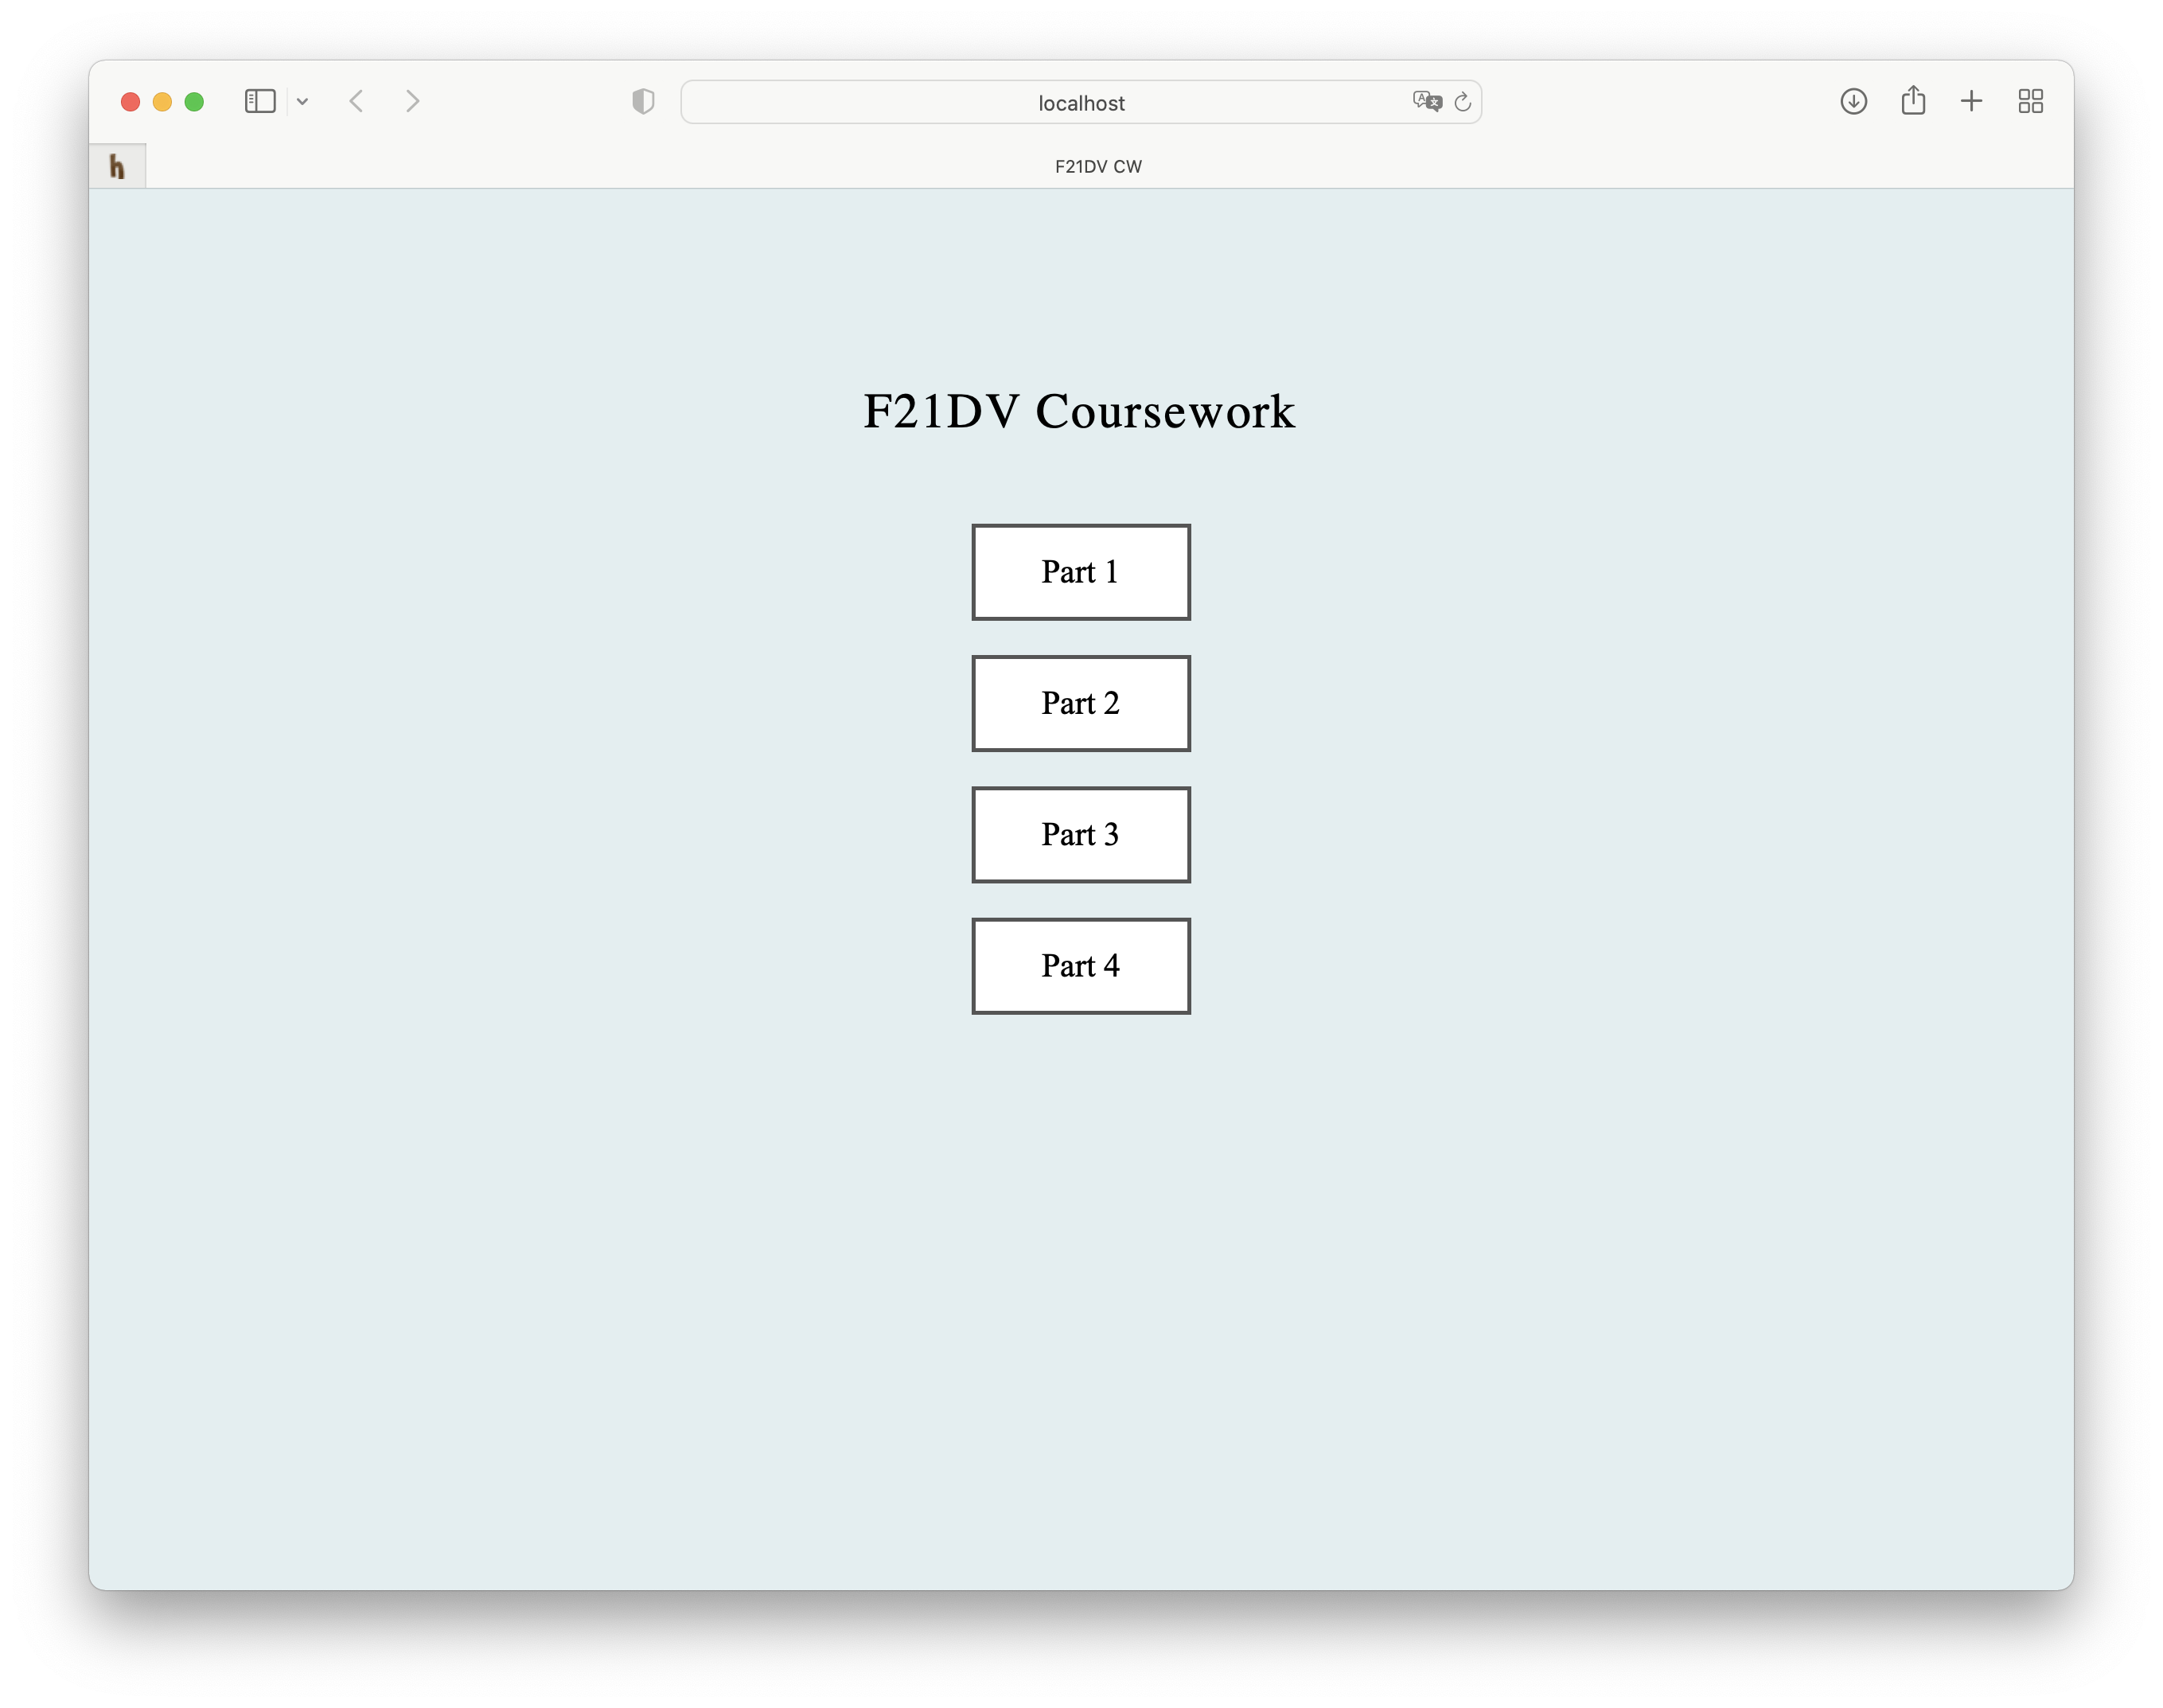
\includegraphics[width = 10cm]{images/main.png}
    \label{fig:main}
    \caption{Main Index Page}
\end{figure}
\FloatBarrier
The main index page of the web application would show buttons to access parts 1 to
4, as shown in figure \ref{fig:main}, and for the case of Lab 1, upon clicking on
the Part 1 button, a series of urls linking to different exercises would be shown,
as seen in figure \ref{fig:part1} below.
\begin{figure}[!ht]
    \centering
    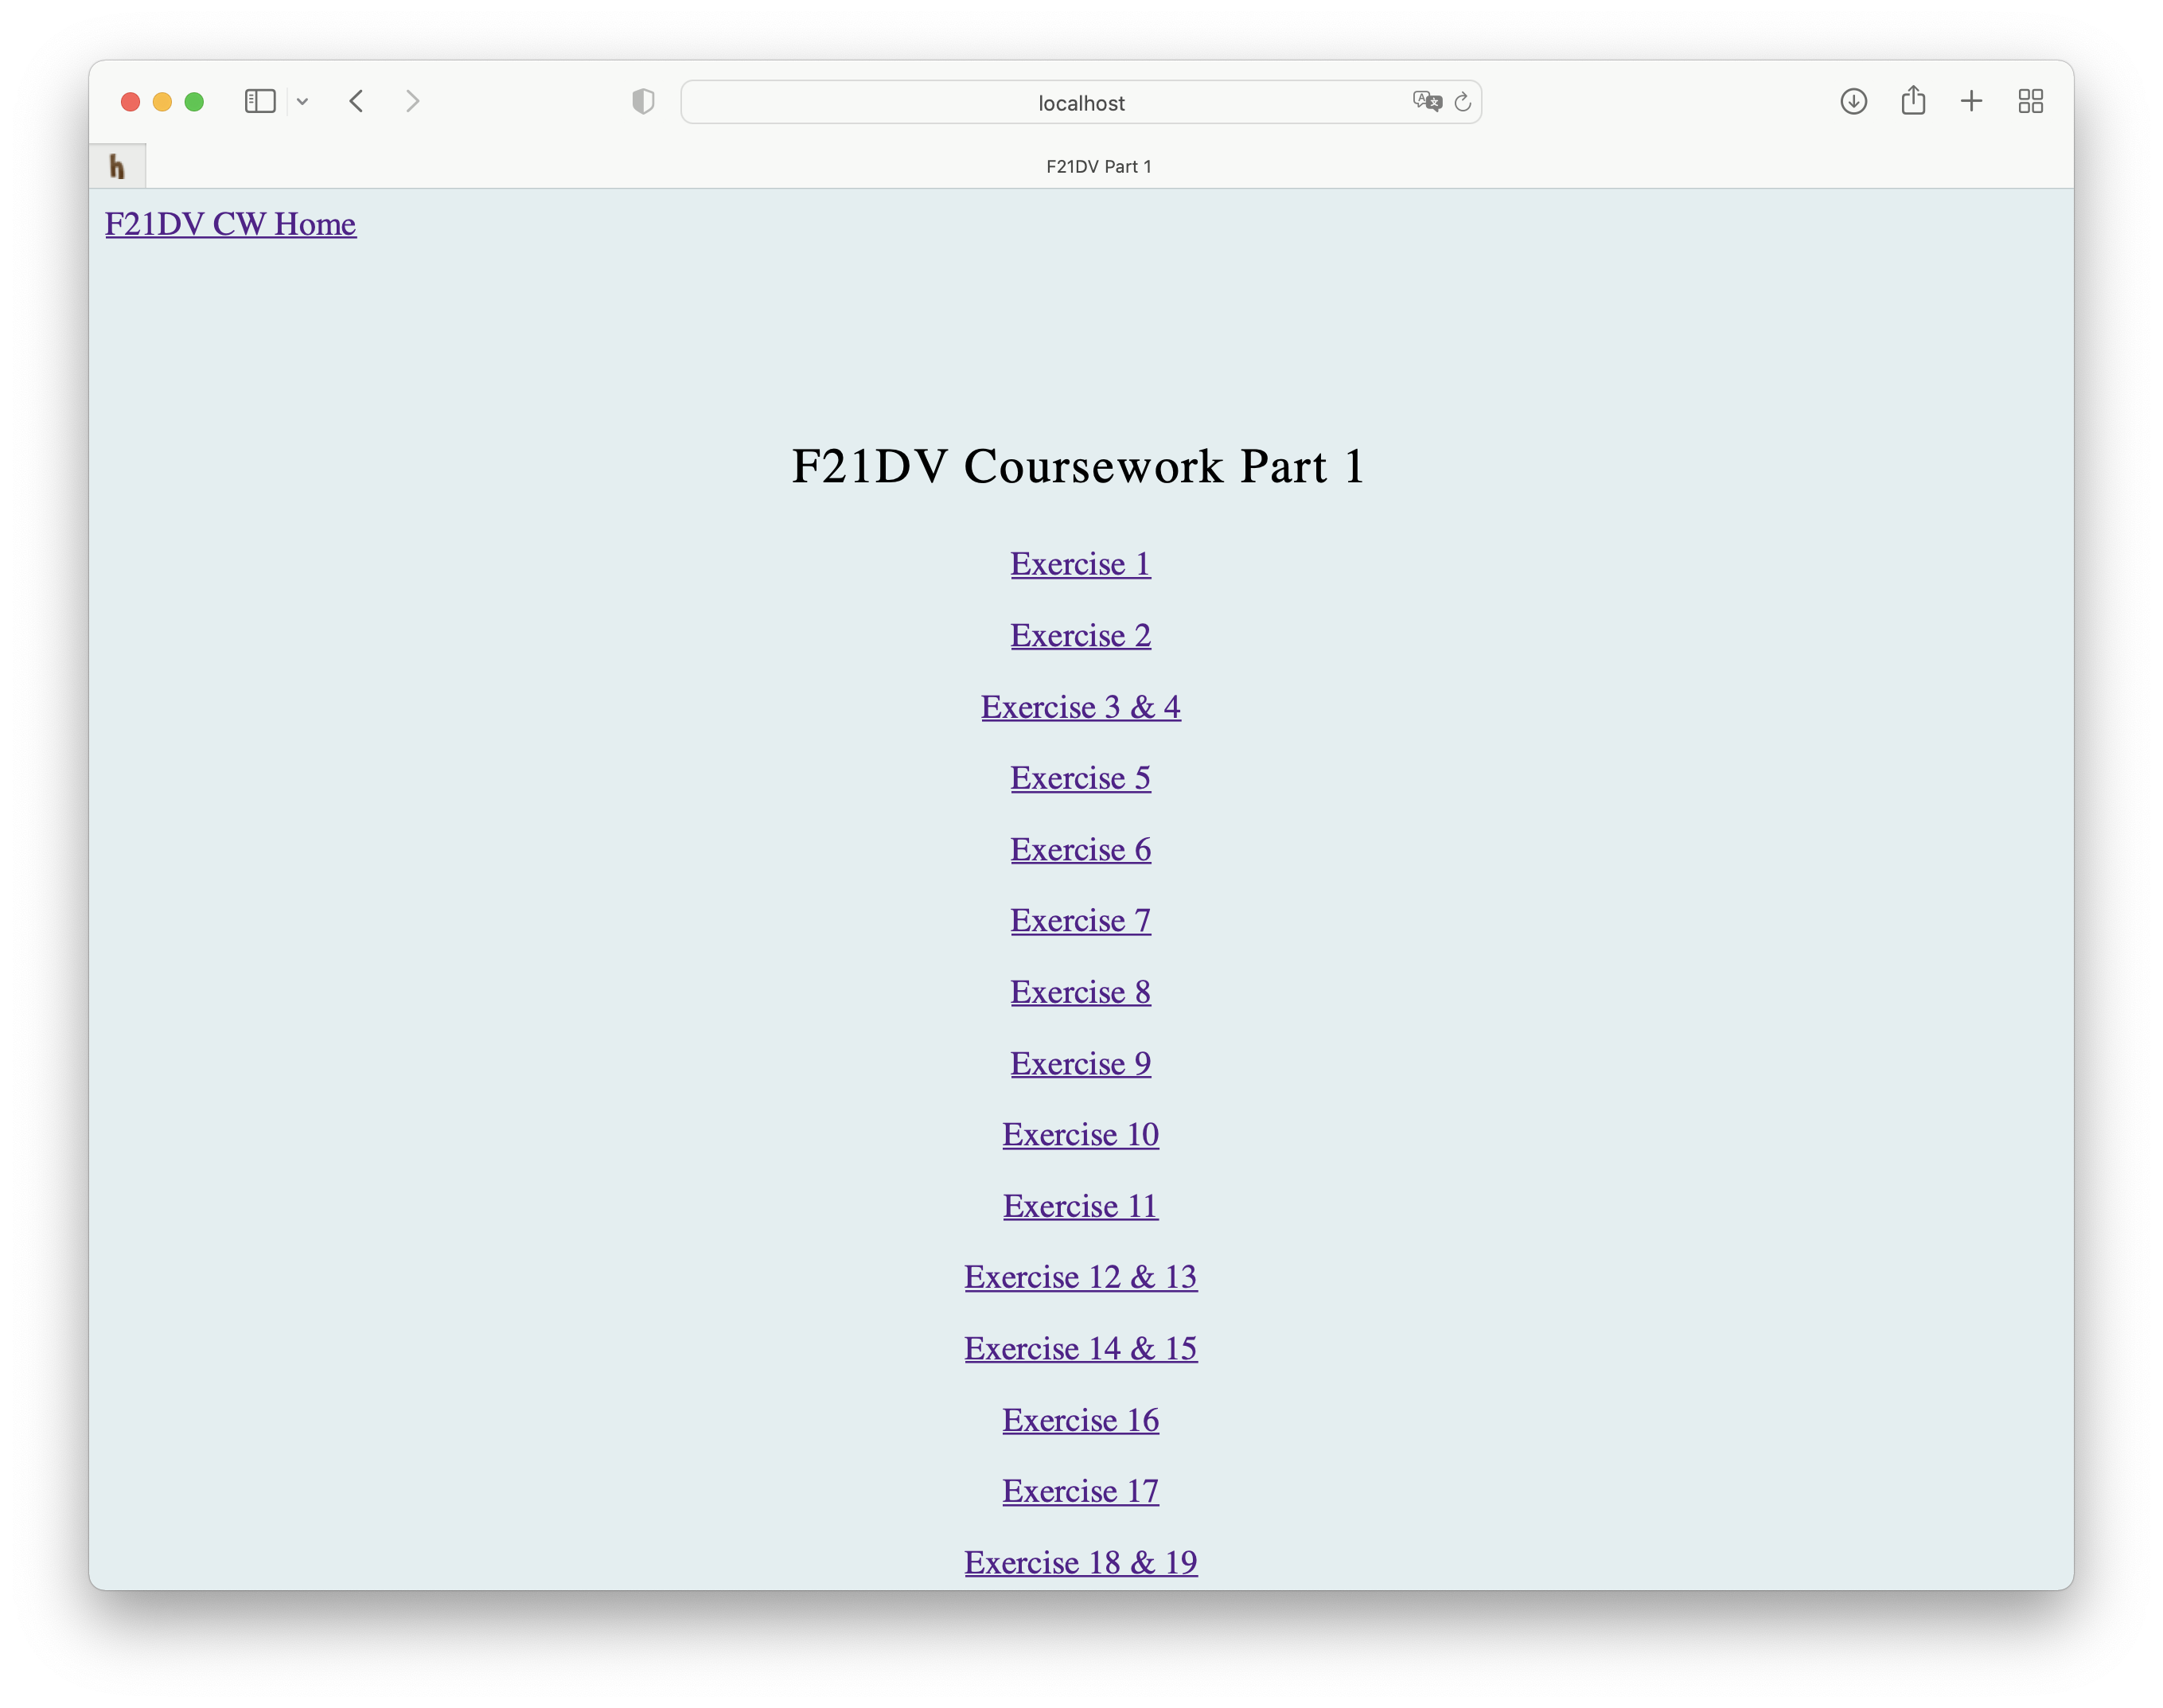
\includegraphics[width = 7cm]{images/part1_1.png}
    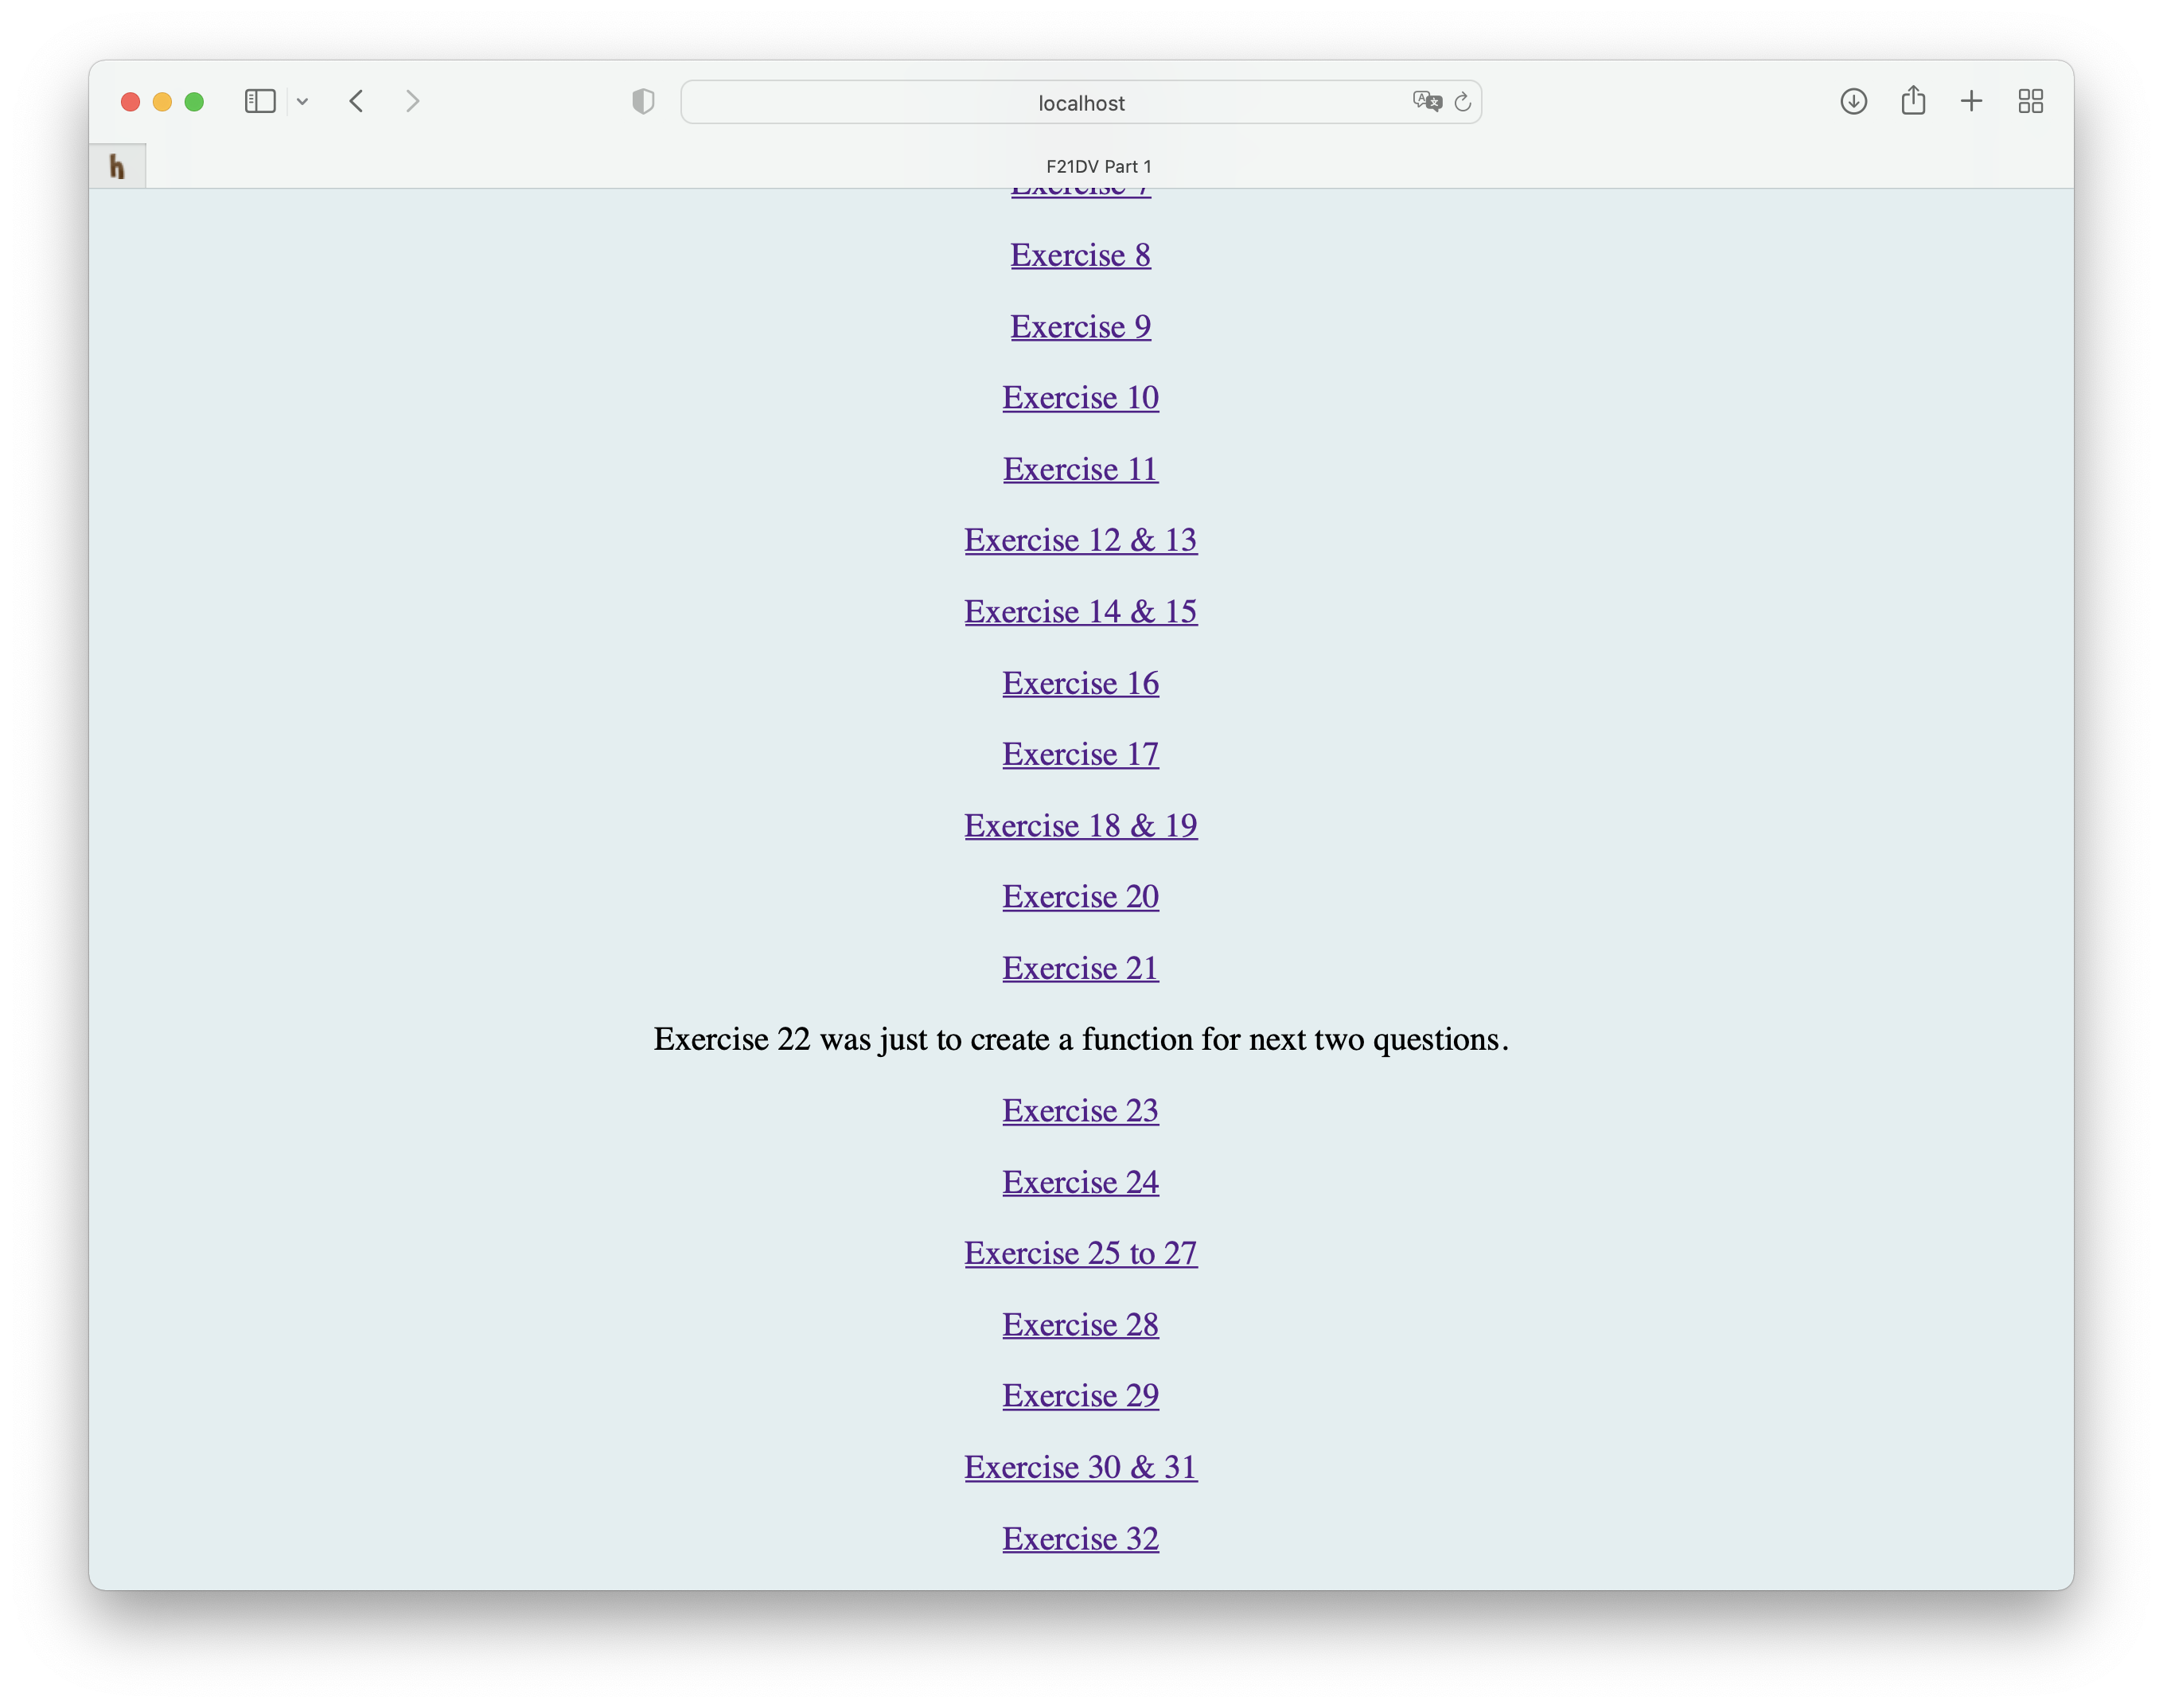
\includegraphics[width = 7cm]{images/part1_2.png}
    \label{fig:part1}
    \caption{Main Index Page}
\end{figure}
\FloatBarrier
To demonstrate the understanding of \verb|d3.js|, this series of URLs were created
systematically using \verb|d3.js|, as shown in listing \ref{lst:urlSystematic} abstact
below. 

\begin{lstlisting}[language=JavaScript,
                    caption={Systematic URL Creation},
                    captionpos=b,
                    label={lst:urlSystematic}]
    // Array of numbers [0, 1, 2, ..., 32] defining number of exercises
    const data = Array.from(Array(33).keys());

    // Creating links to 32 Exercises Systematically.
    d3.select('body').selectAll('p')
        .data(data)
        .enter()
            // Append a <p> for each exercise and add an <a> for each <p>
            .append('p').style('text-align', 'center')
                .attr('class', d => 'task' + d)
                .append('a')
                    .attr('href', d => 'task' + d +'.html')
                    .html(d => 'Exercise ' + d);
\end{lstlisting}

As the lab exercise would involve certain combinable exercises, such as exercises 30
and 31, I have also created a generalised function to help \textbf{combine} and
\textbf{delete} certain exercises.\\

\begin{lstlisting}[language=JavaScript,
    caption={Systematic URL Removal},
    captionpos=b,
    label={lst:taskSystematic}]
    /**
    * General Merge Function. If its just 2 consecutive exercise, ignore 3rd and 4th parameter. 
    * However, if merge is for a range of exercises, spanning more than 2, only enter the 
    * first and last exercise number.
    * @param {*} first first exercise to merge
    * @param {*} second second exercise to merge. Last exercise if there are more than 2 exercises.
    * @param {*} cond1 used to change exercise <number> to Exercise <number> to <number>
    * @param {*} cond2 used to rename html file to task<first>n<second>.html
    */
   function mergeTask(first, second, cond1 = ' \& ', cond2 = 'n') {
       d3.select('.task' + second).remove();
       d3.select('.task' + first + ' a').html('Exercise ' + first + cond1 + second)
                                           .attr('href', d => 'task' + first + cond2 + second + '.html');
   }
\end{lstlisting}
Listing \ref{lst:taskSystematic} shows a function that renames the href of combined exercises,
and removes and rename a pre-existing href. For example, we have initially Exercises 30 and 31.
The function first removes the exercise 31's \verb|<p>|, and then renames the original html href file
from \verb|task30.html| to \verb|task30n31.html|.\\

\begin{lstlisting}[language=JavaScript,
    caption={Systematic <a>-text Replacement},
    captionpos=b,
    label={lst:divReplaceSystematic}]
    // Remove task function
    function removeTask(task, message) {
        d3.select(`.task${task} a`).remove();
        d3.select(`.task${task}`).append('p')
                                .text(message);
    }
\end{lstlisting}
Listing \ref{lst:divReplaceSystematic} shows a generalised function that replaces the exercises URL
with a message string. For example, in exercise 22, we were asked to create a generalised SVG and
lines function. This function will now remove the \verb|href| from the \verb|<p>| element, and replace
it with a message string.


\newpage
\section{Individual Exercise HTMLs Setup}
Within each exercise's own HTML \verb|body|, they all inherit a generic CSS setting for a div called
\verb|.answerCenter| which acts as the center element for the presentation of answers for each
exercise. There is also a generic button cssd style called \verb|.buttonOri| and \verb|.button| that
handles the CSS transition of all the buttons. \\
\par For each exercise, I have also used a generalised function in \verb|functions.js| to create the
\verb|<div>|s and buttons so that the styles remain consistent across all exercises.\\
\begin{lstlisting}[language=JavaScript,
    caption={Systematic div and button creation},
    captionpos=b,
    label={lst:functionsjs}]
    /**
    * Create div's for each question systematically.
    * @param {*} exerciseNumber Task number.
    */
   export function createDiv(exerciseNumber) {
       d3.select('body')
           .append('div')
               .attr('class', 'container')
               .append('div')
                   .attr('class', 'answerCenter')
                   .append('p')
                       .append('strong')
                           .text('Exercise ' + exerciseNumber + ':')
   }
   
   /**
    * Creates a button to execute action for each task.
    * @param {*} exerciseNumber 
    */
   export function createButton(exerciseNumber) {
       d3.select('body')
           .append('div').attr('class', 'container')
               .append('div').attr('class', 'center')
                   .append('button')
                       .attr('class', 'buttonori')
                       .text('Click for Task ' + exerciseNumber)
   }
\end{lstlisting}
Listing \ref{lst:functionsjs} shows the systematic approach used to create the answer container, 
as well as buttons to execute exercises actions. However, not all exercise would use the button,
since not all exercise is in need of an action.

\newpage
\chapter{Exercises}
\section{Exercise 1}
\begin{figure}[!ht]
    \centering
    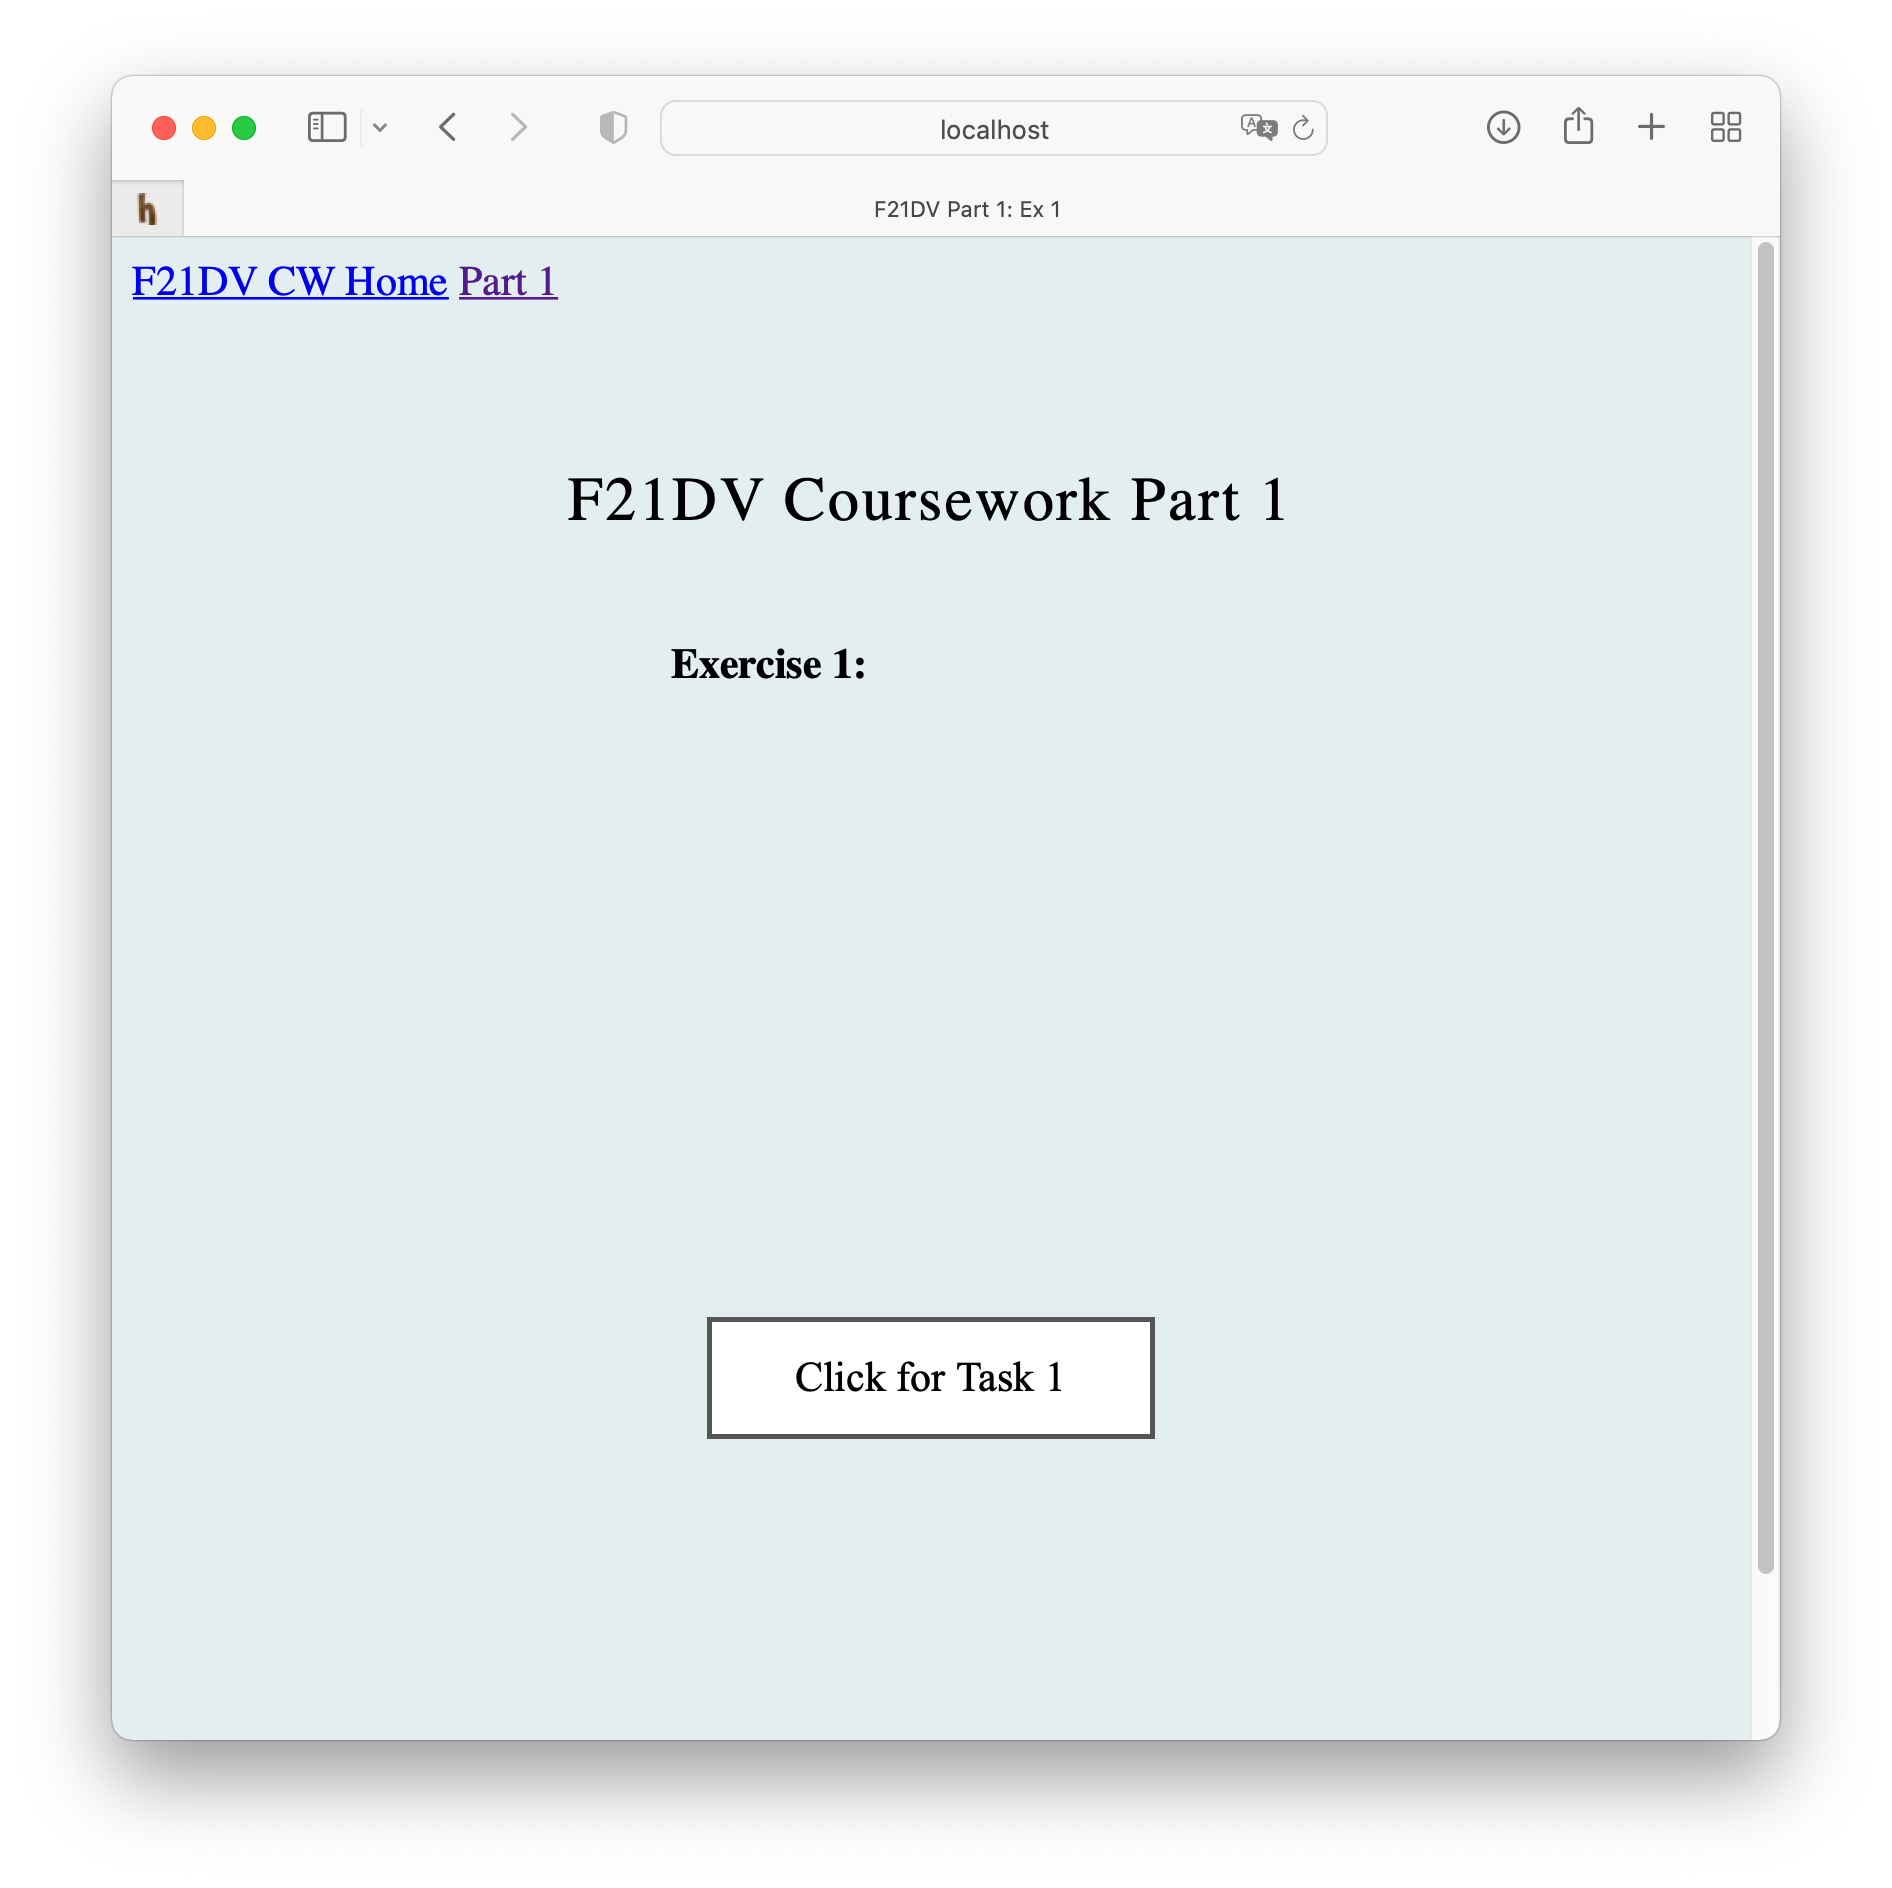
\includegraphics[width = 7.5cm]{images/ex1_1.png}
    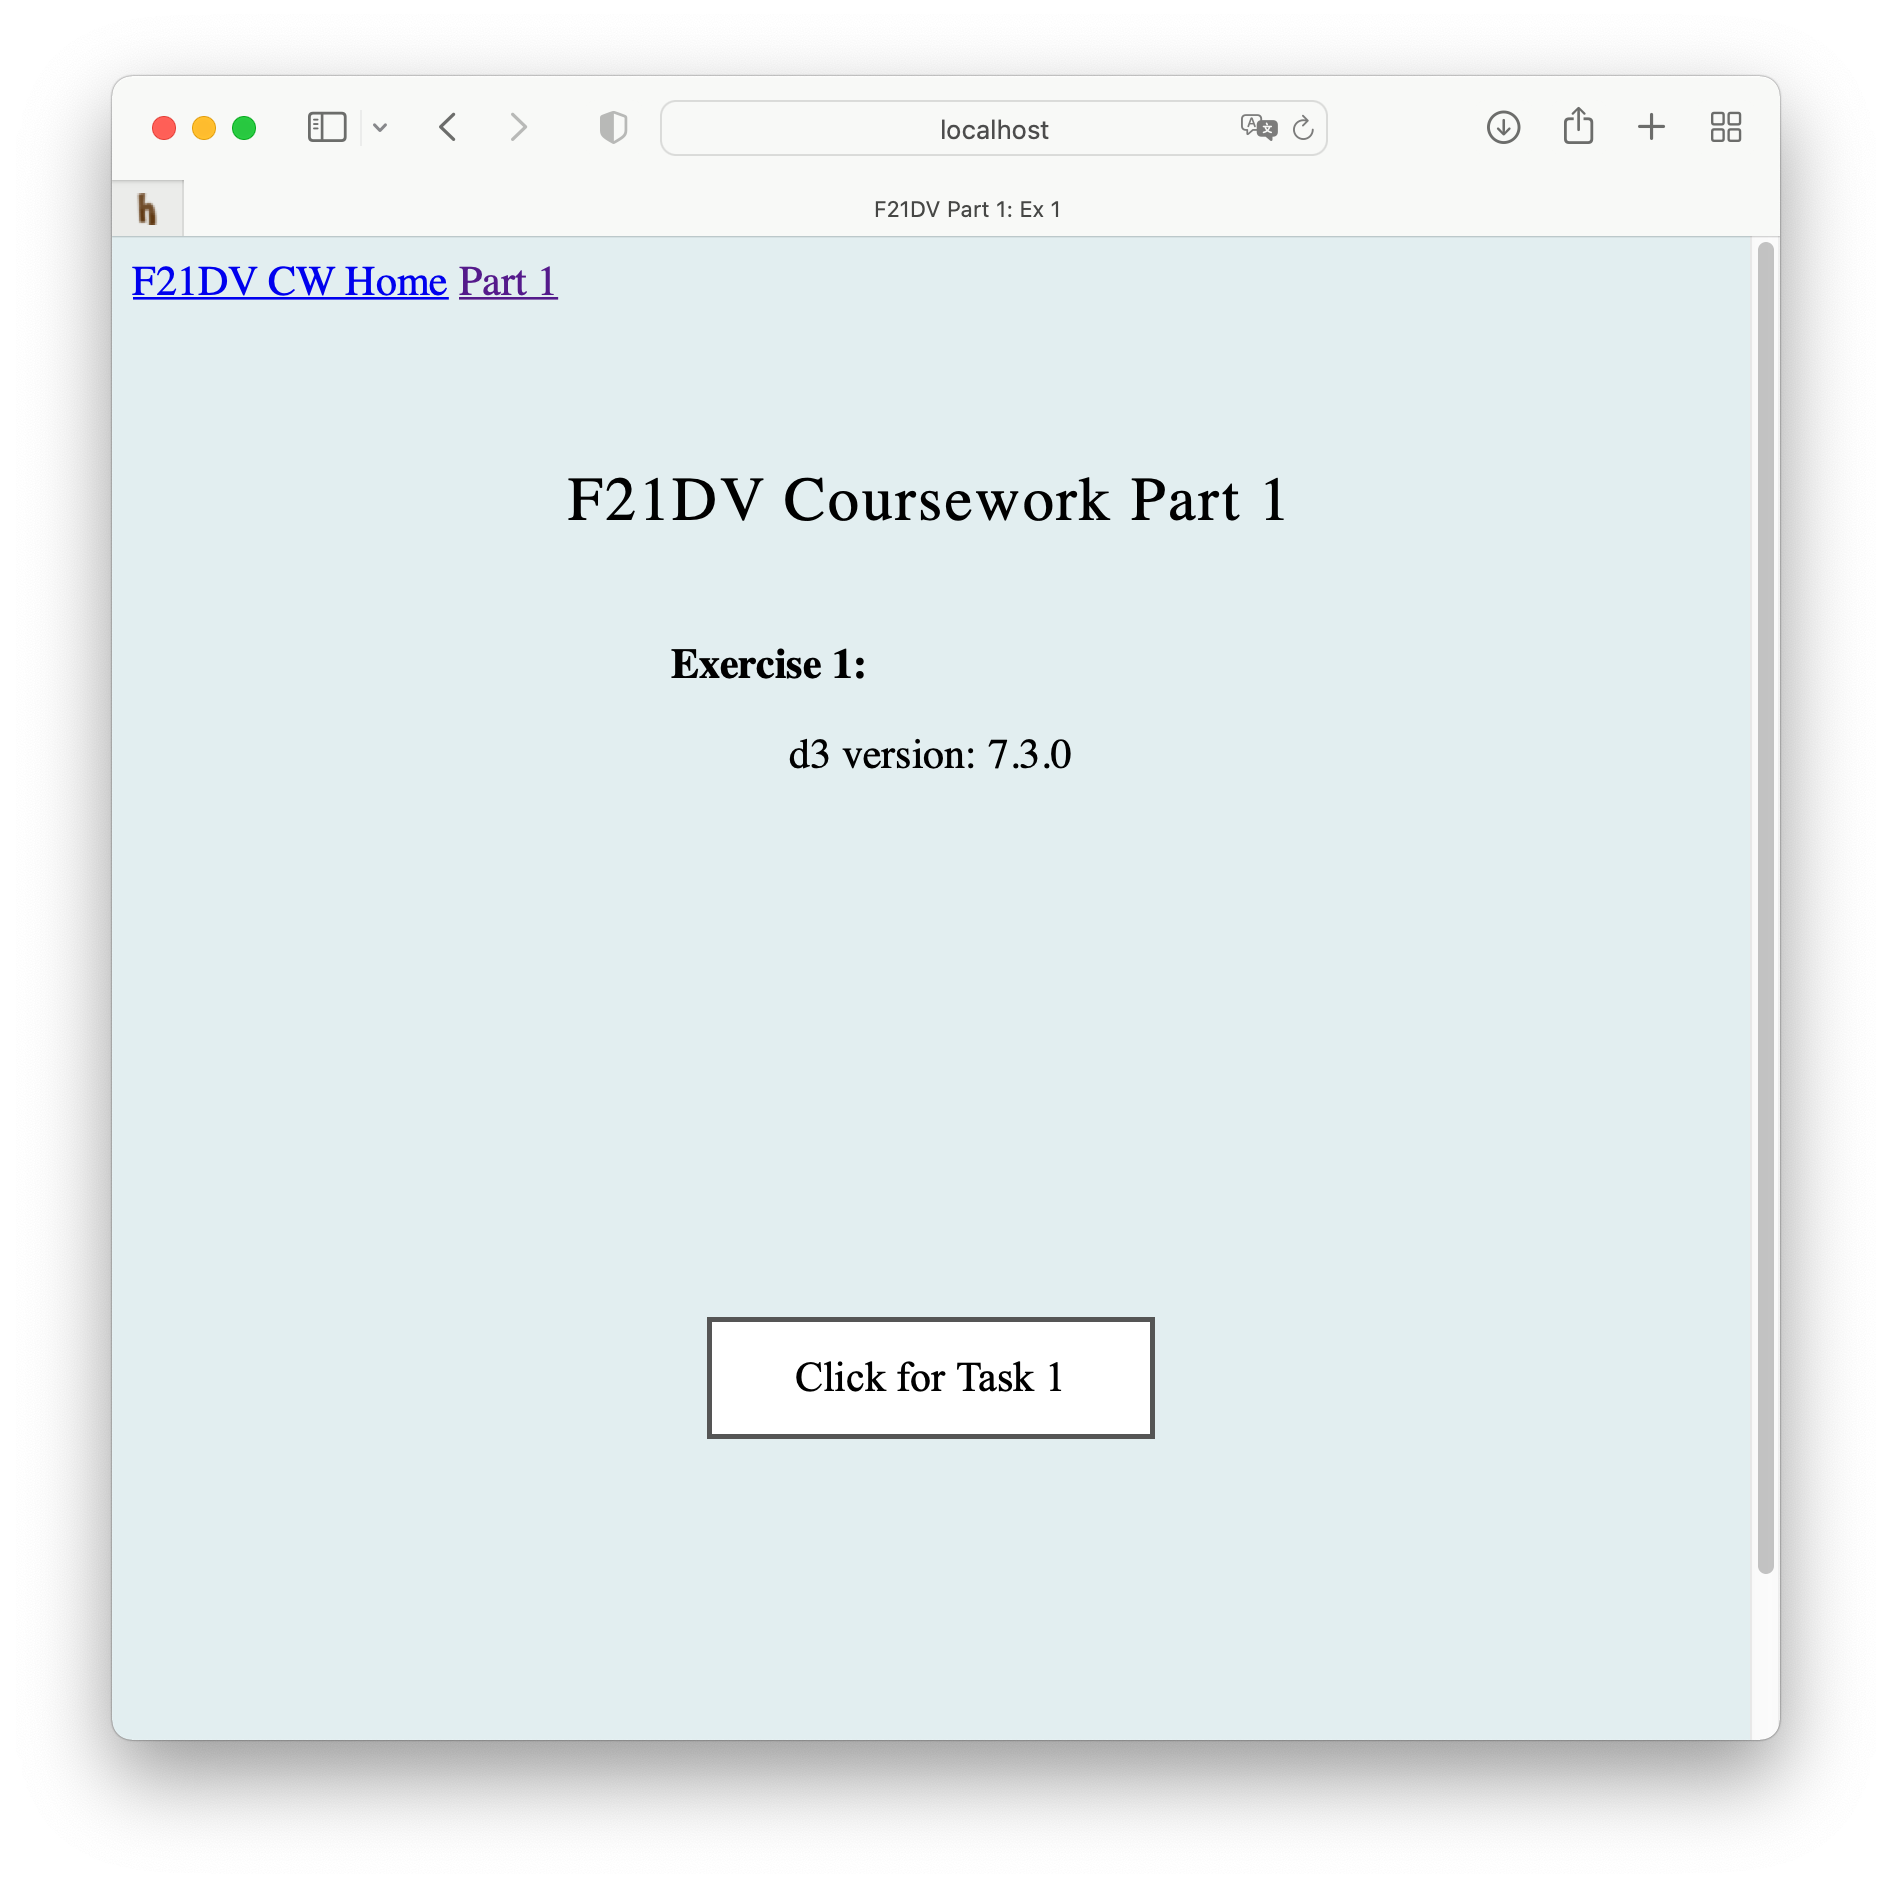
\includegraphics[width = 7.5cm]{images/ex1_2.png}
    \label{fig:ex1}
    \caption{Exercise 1}
\end{figure}
\FloatBarrier
Figure \ref{fig:ex1} shows the outcome after clicking on the action button. The answer container
space would print the d3 version number upon clicking the task button.
\lstinputlisting[language=JavaScript]{../../public/js/part1/task1.js}
Upon clicking the button, using d3, the button action replaces the empty \verb|<p>| with "d3
version: 7.3.0". For the remaining exercises, the button action would do a similar thing as well.
It would select the desired object for modification, and through a button on-click event listener,
modify the selected object.

\newpage
\section{Exercise 2}
\begin{figure}[!ht]
    \centering
    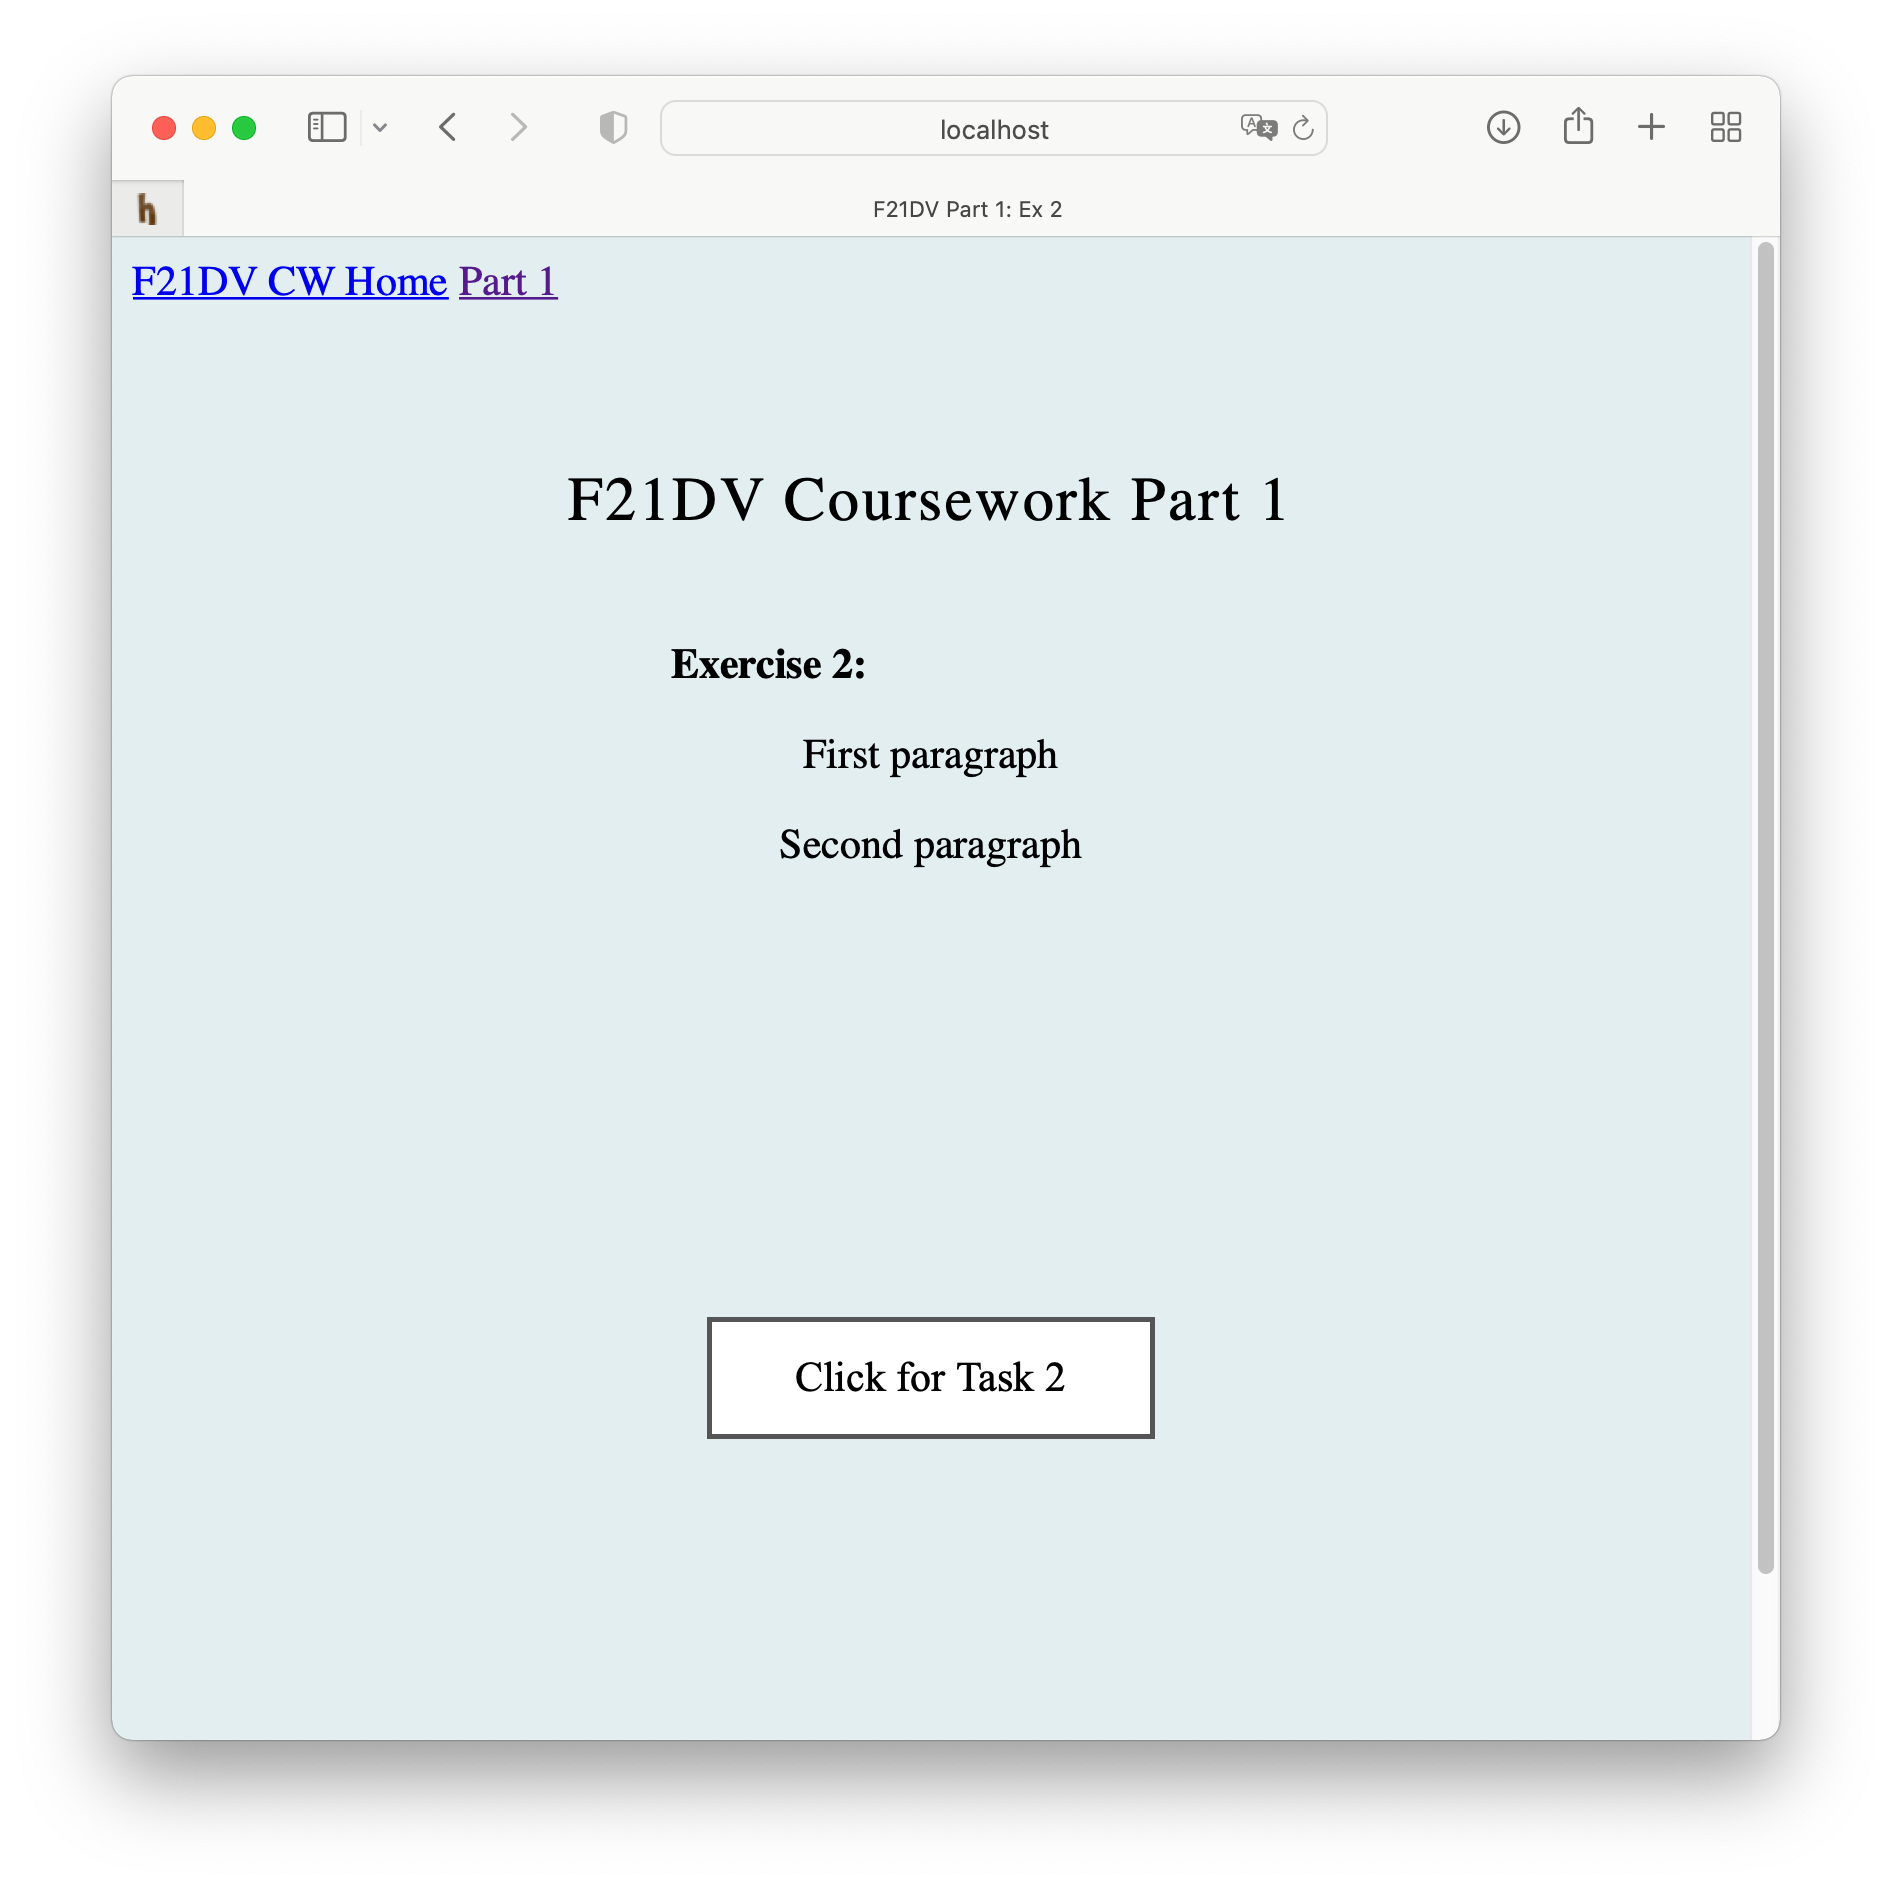
\includegraphics[width = 8cm]{images/ex2_1.png}
    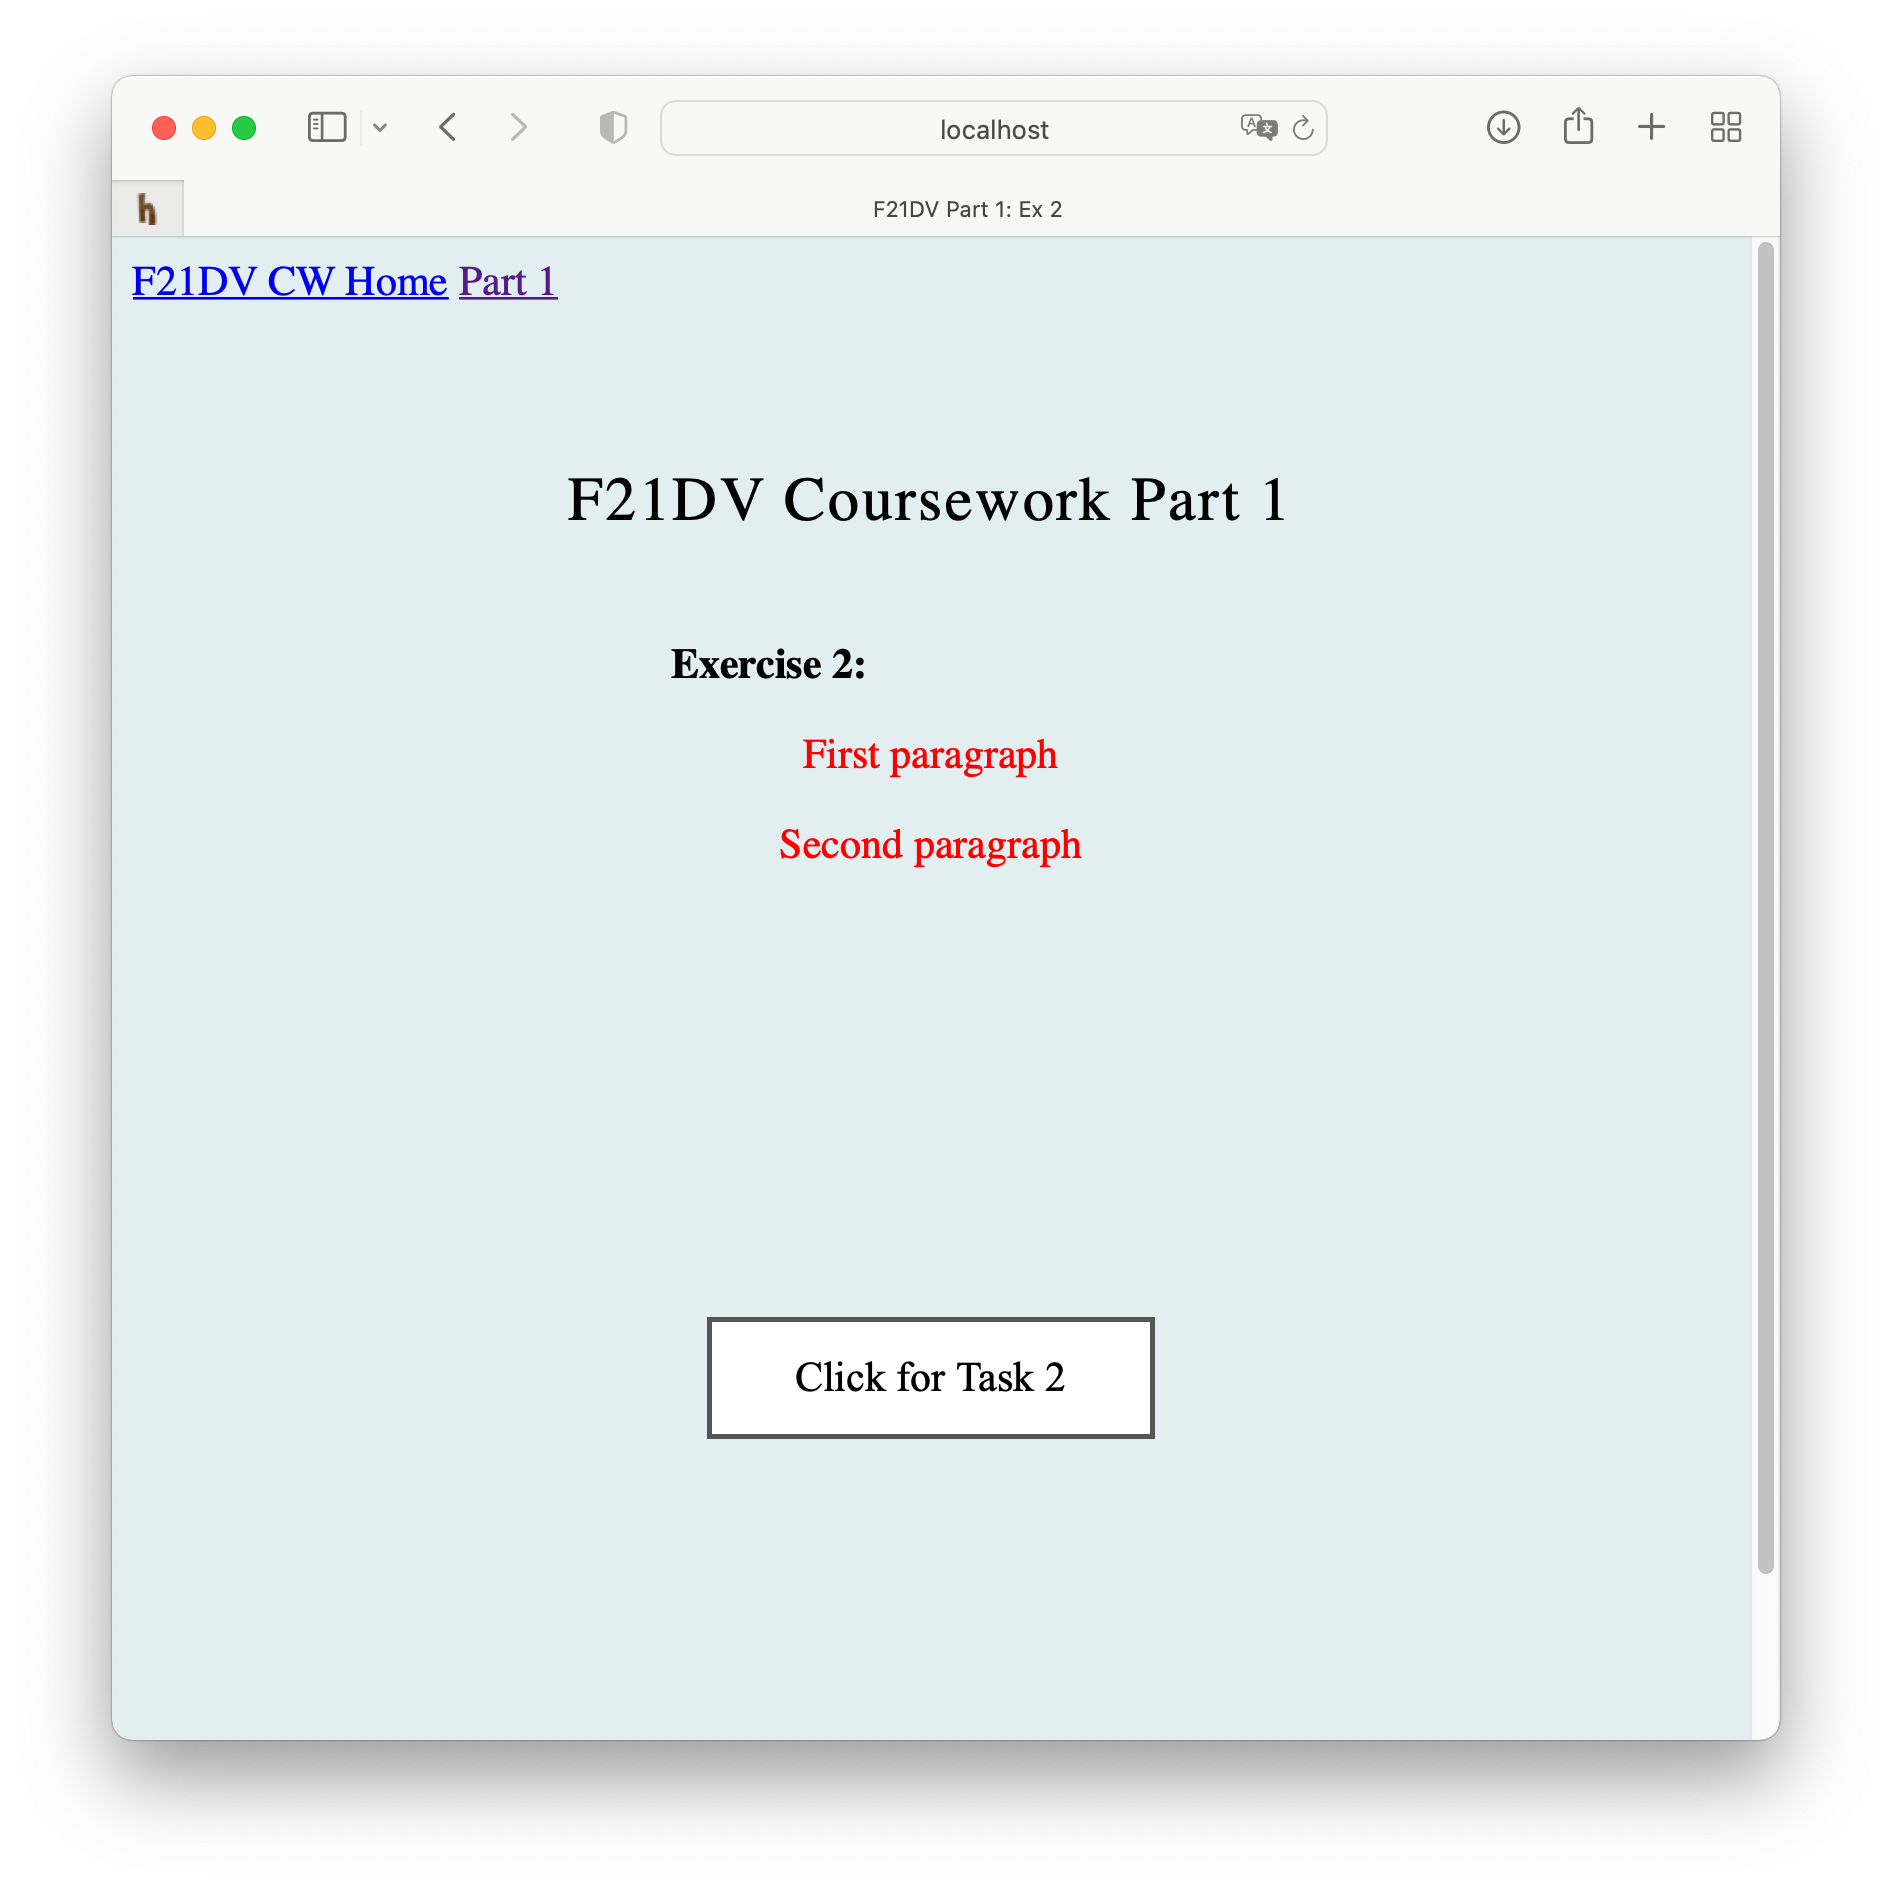
\includegraphics[width = 8cm]{images/ex2_2.png}
    \label{fig:ex2}
    \caption{Exercise 2}
\end{figure}
\FloatBarrier
Figure \ref{fig:ex2} shows that upon clicking the button, d3 would change the colours of the selected
\verb|<p>|s to red. 

\newpage
\section{Exercise 3 \& 4}
Exercises 3 \& 4 are one of the exercises where I have combined into one.
\begin{figure}[!ht]
    \centering
    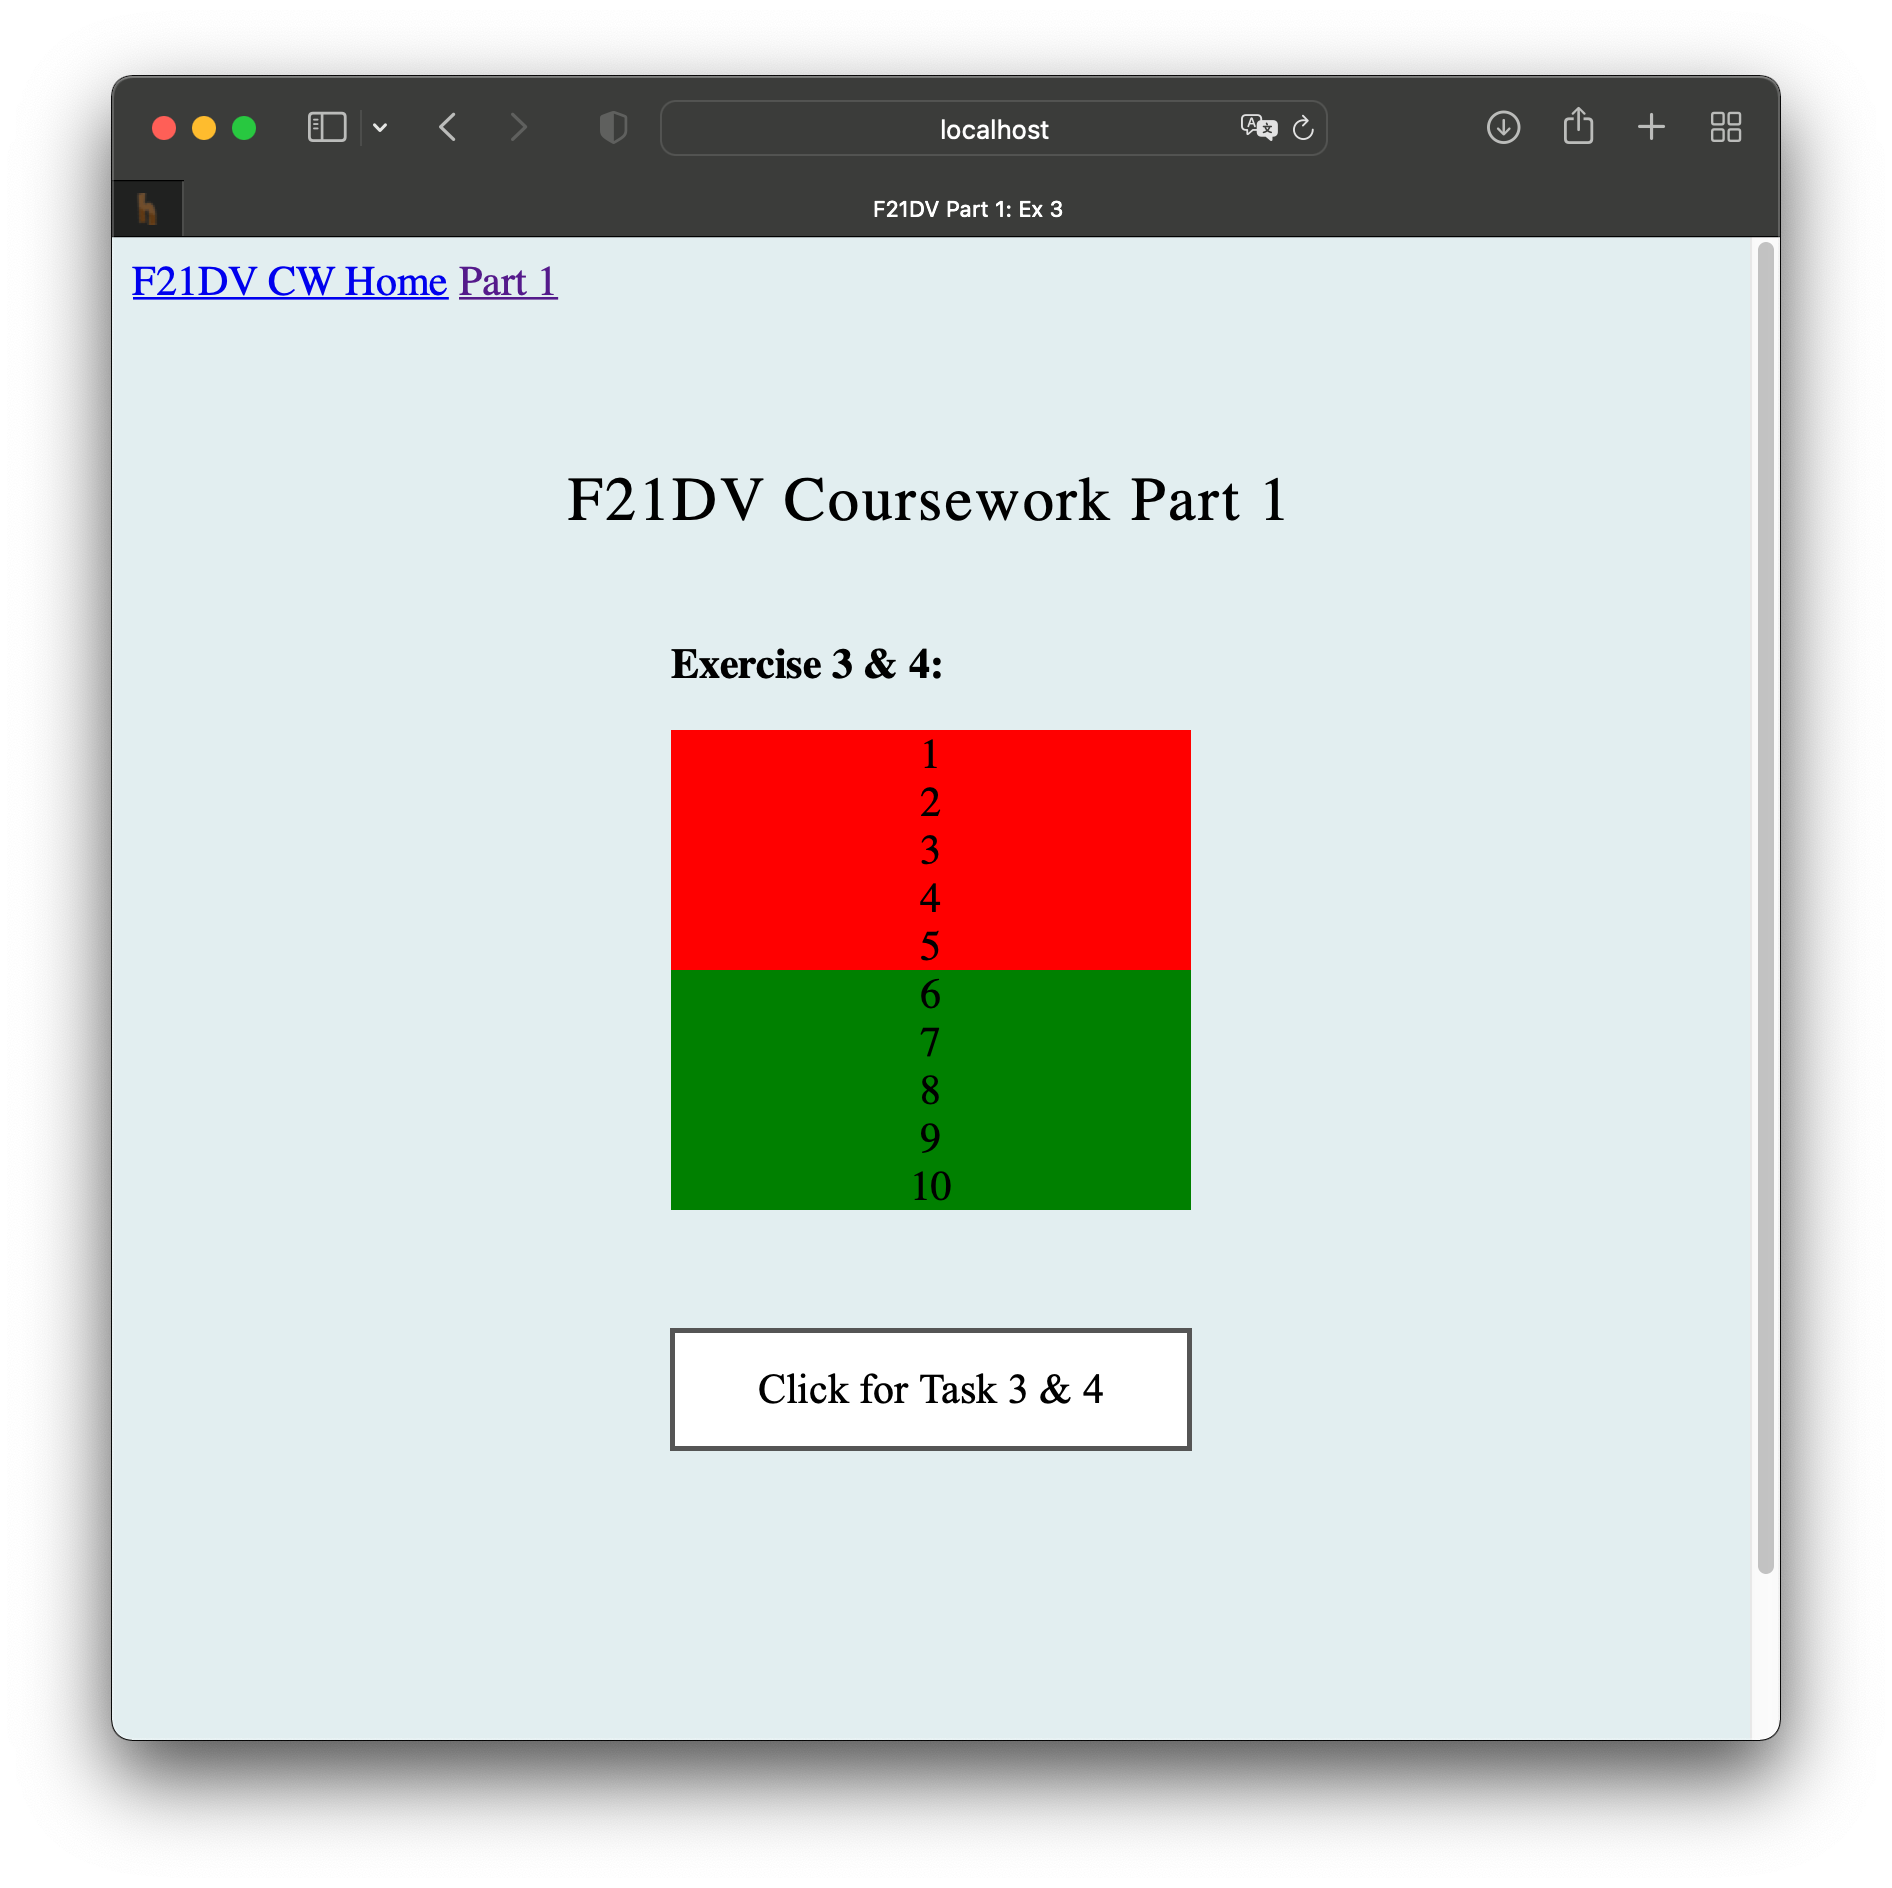
\includegraphics[width = 8cm]{images/ex3_1.png}
    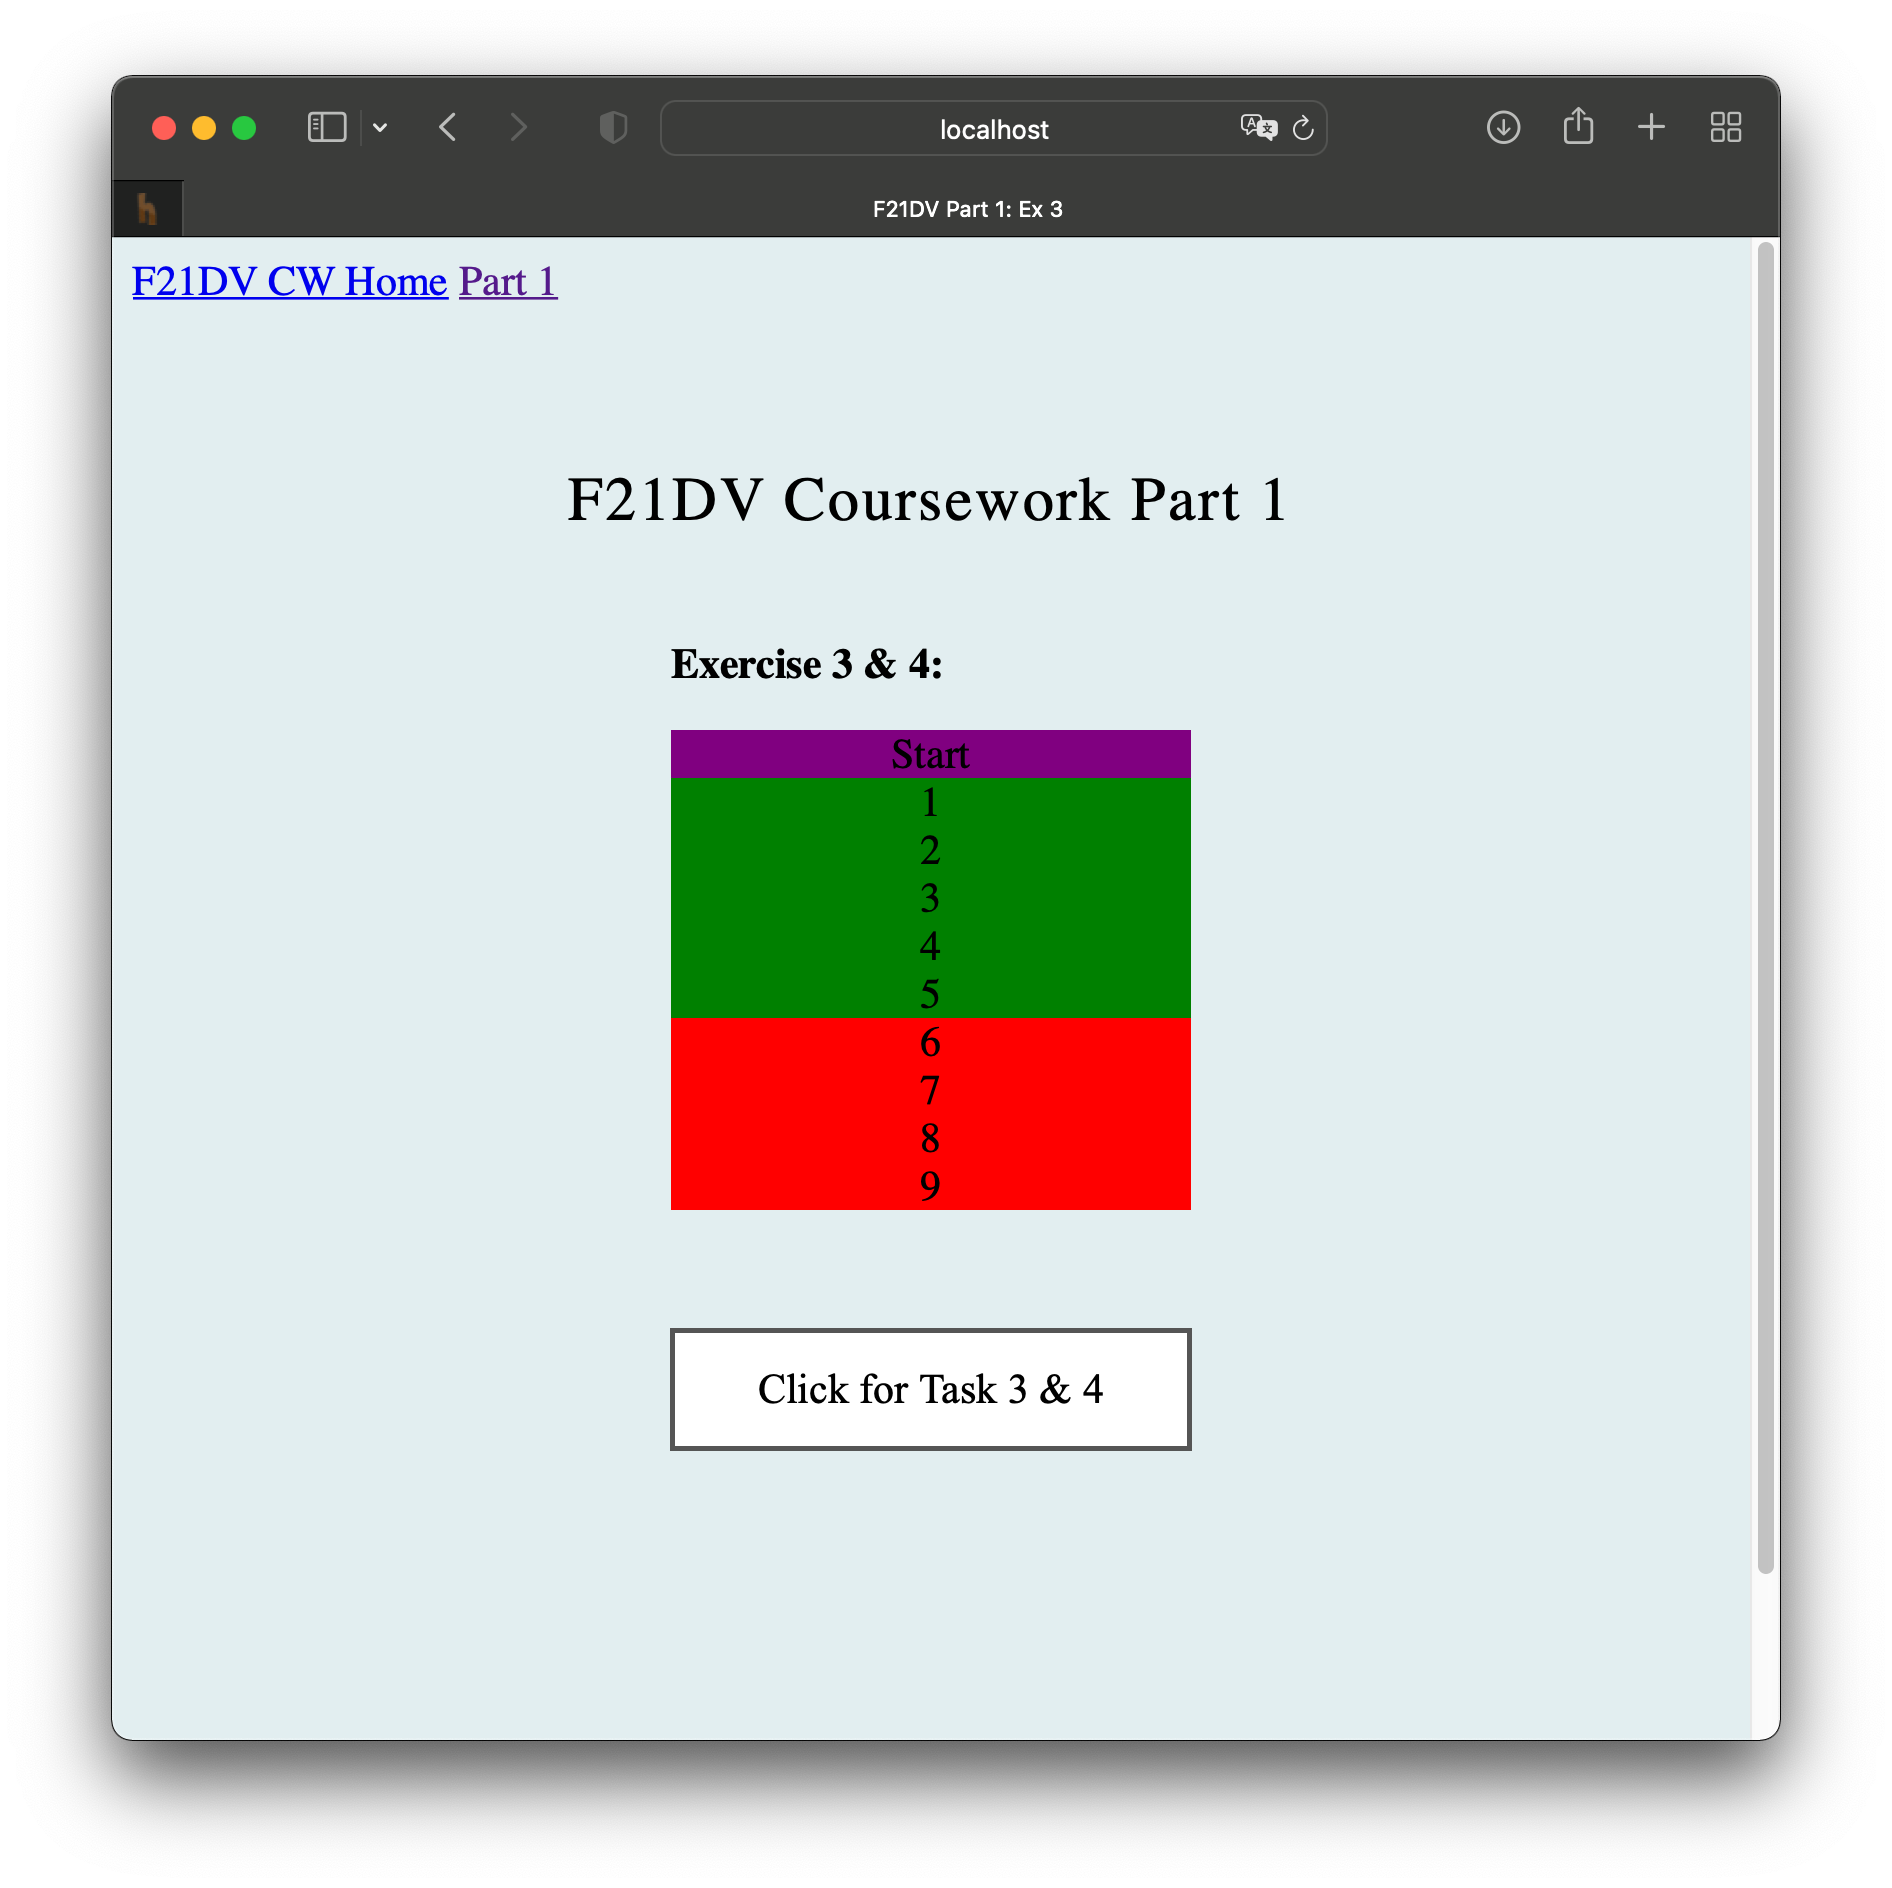
\includegraphics[width = 8cm]{images/ex3_2.png}
    \label{fig:ex3}
    \caption{Exercise 3}
\end{figure}
\FloatBarrier
Exercise 3 was to populate 10 div elements with numbers from 1 to 10, and to colour them according to
their values. Task four asks then, to replace the first value, ``1", with the text ``start". However, I
went ahead and implemented the change for the remaining divs as well, changing their values so that
the divs would show start, 1, 2, ..., 9, whilst keeping the colour requirements. Upon clicking the
button, the state of the div's would return to the original state again. Button is clickable multiple
times.

\newpage
\section{Exercise 5}
\begin{figure}[!ht]
    \centering
    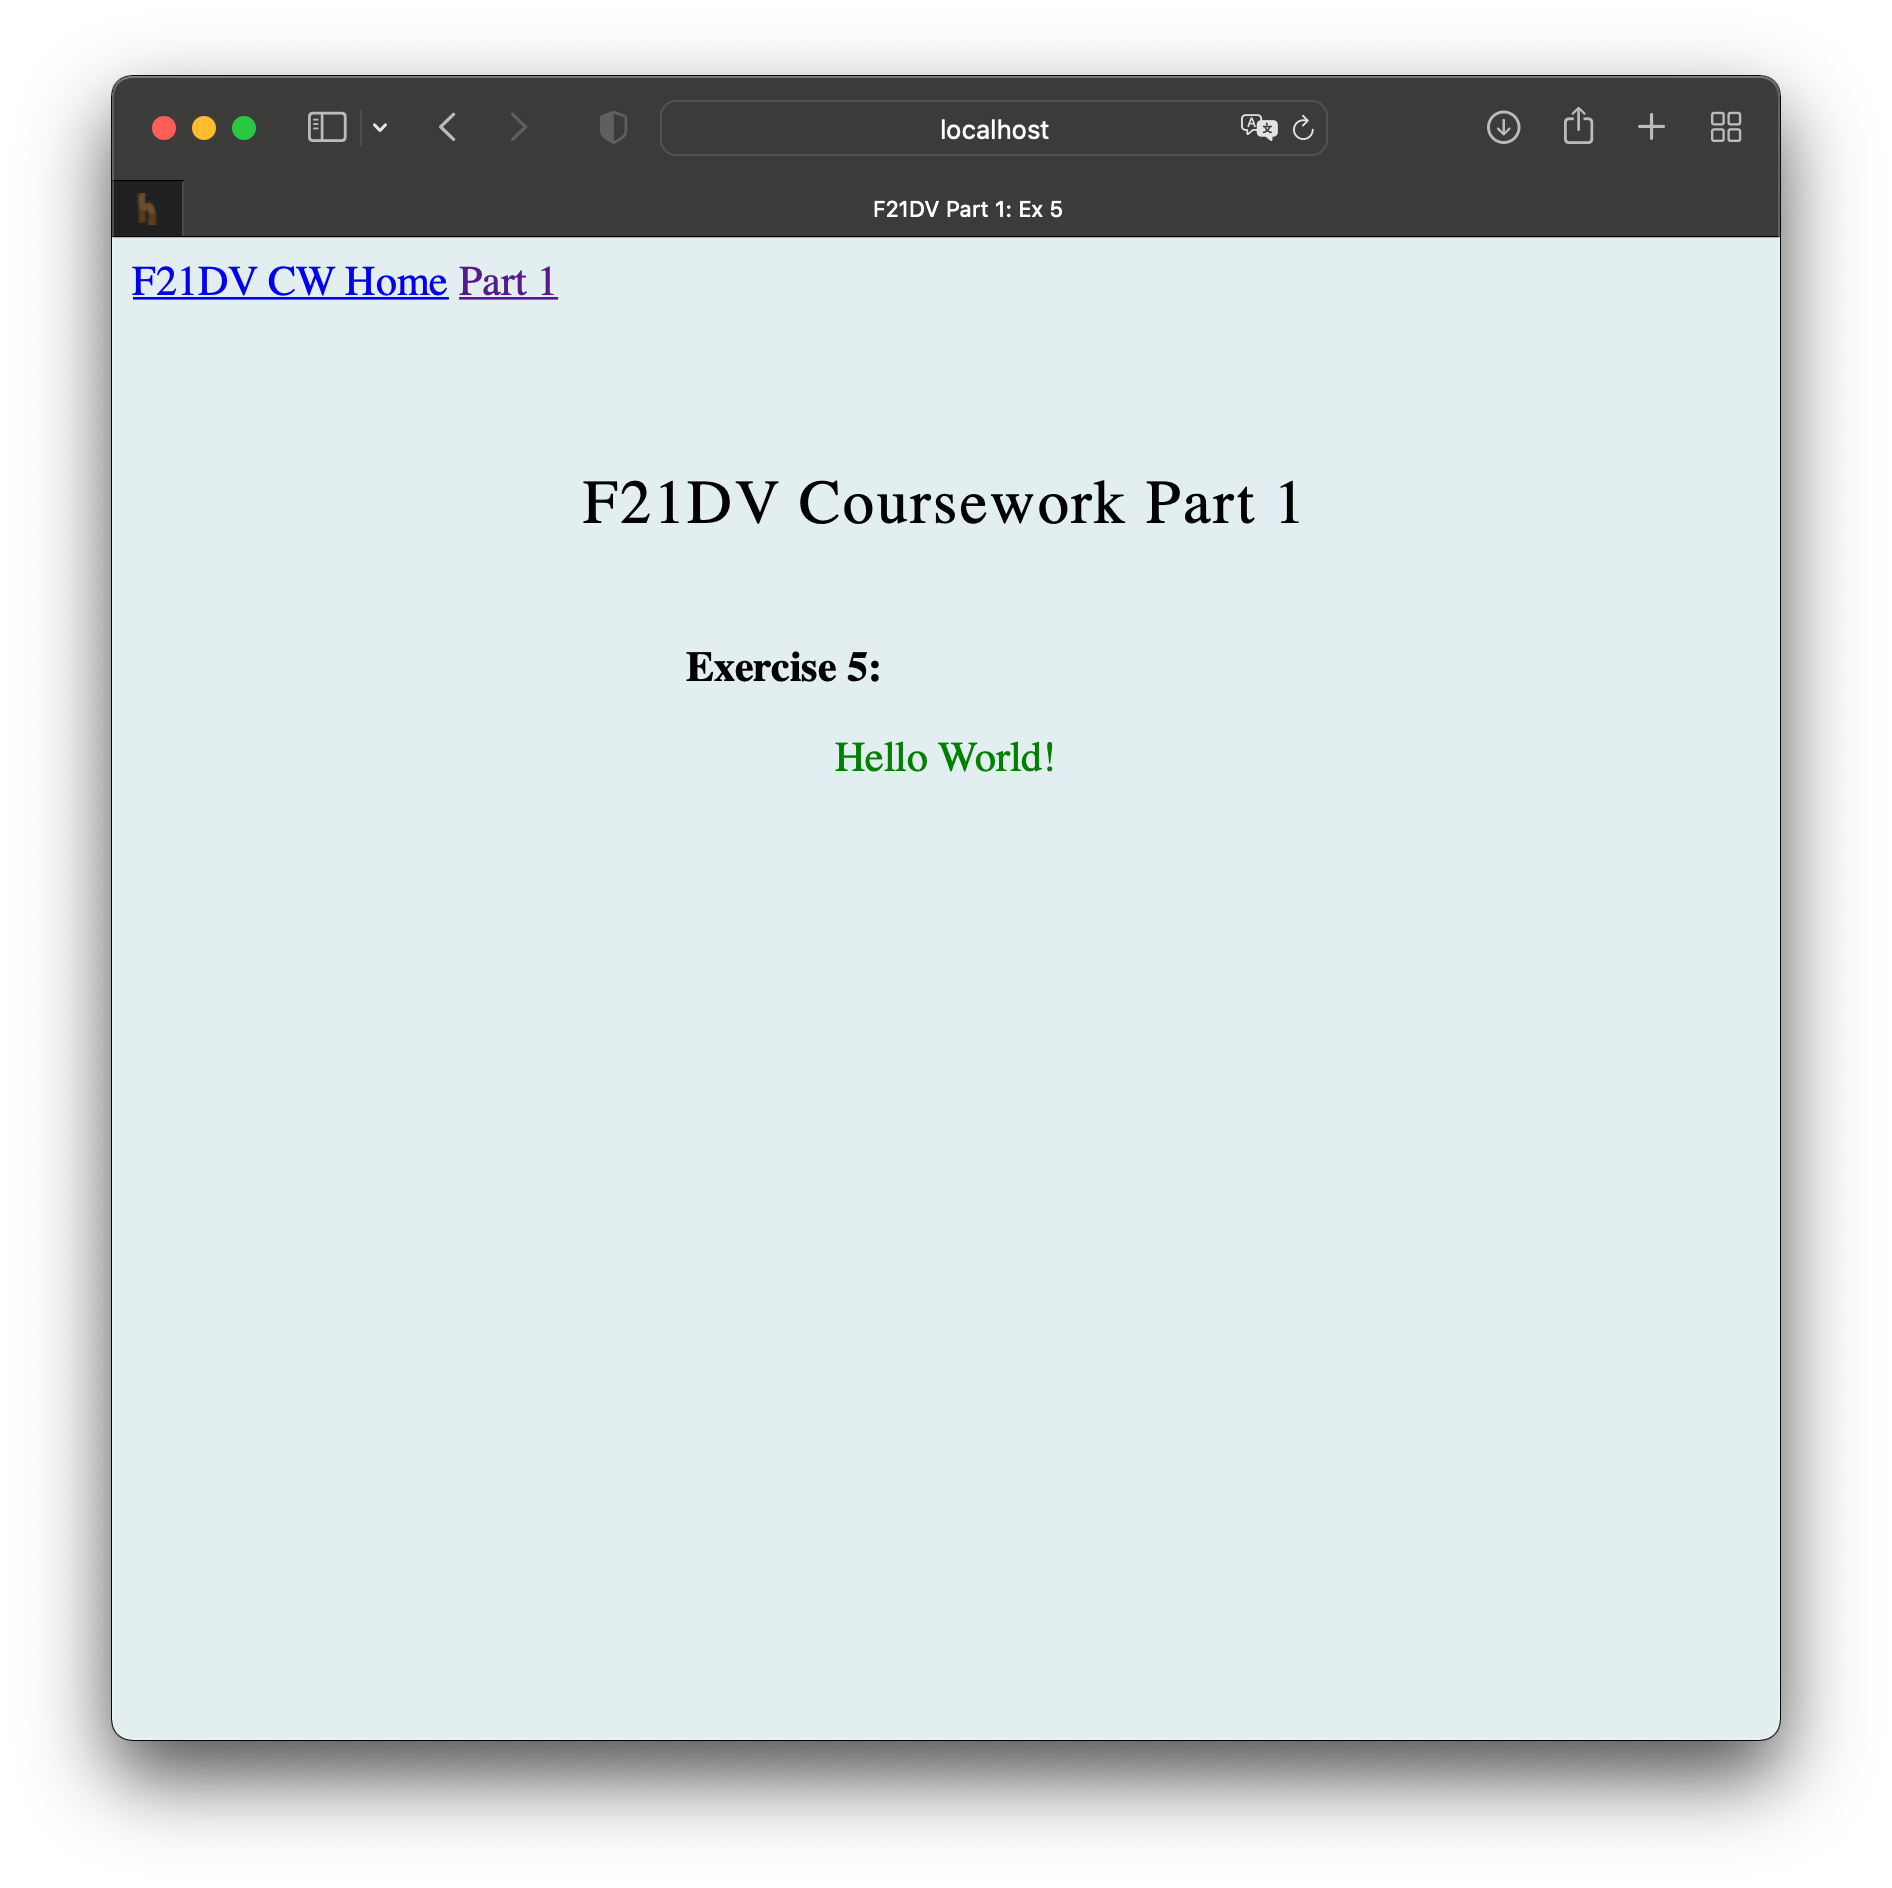
\includegraphics[width = 8cm]{images/ex5.png}
    \label{fig:ex5}
    \caption{Exercise 5}
\end{figure}
\FloatBarrier
\lstinputlisting[language=JavaScript]{../../public/js/part1/task5.js}
Exercise 5 shows a chained d3 syntax where d3 appends a div, adds a text and changes the text colour
to green all in one go.

\newpage
\section{Exercise 6}
\begin{figure}[!ht]
    \centering
    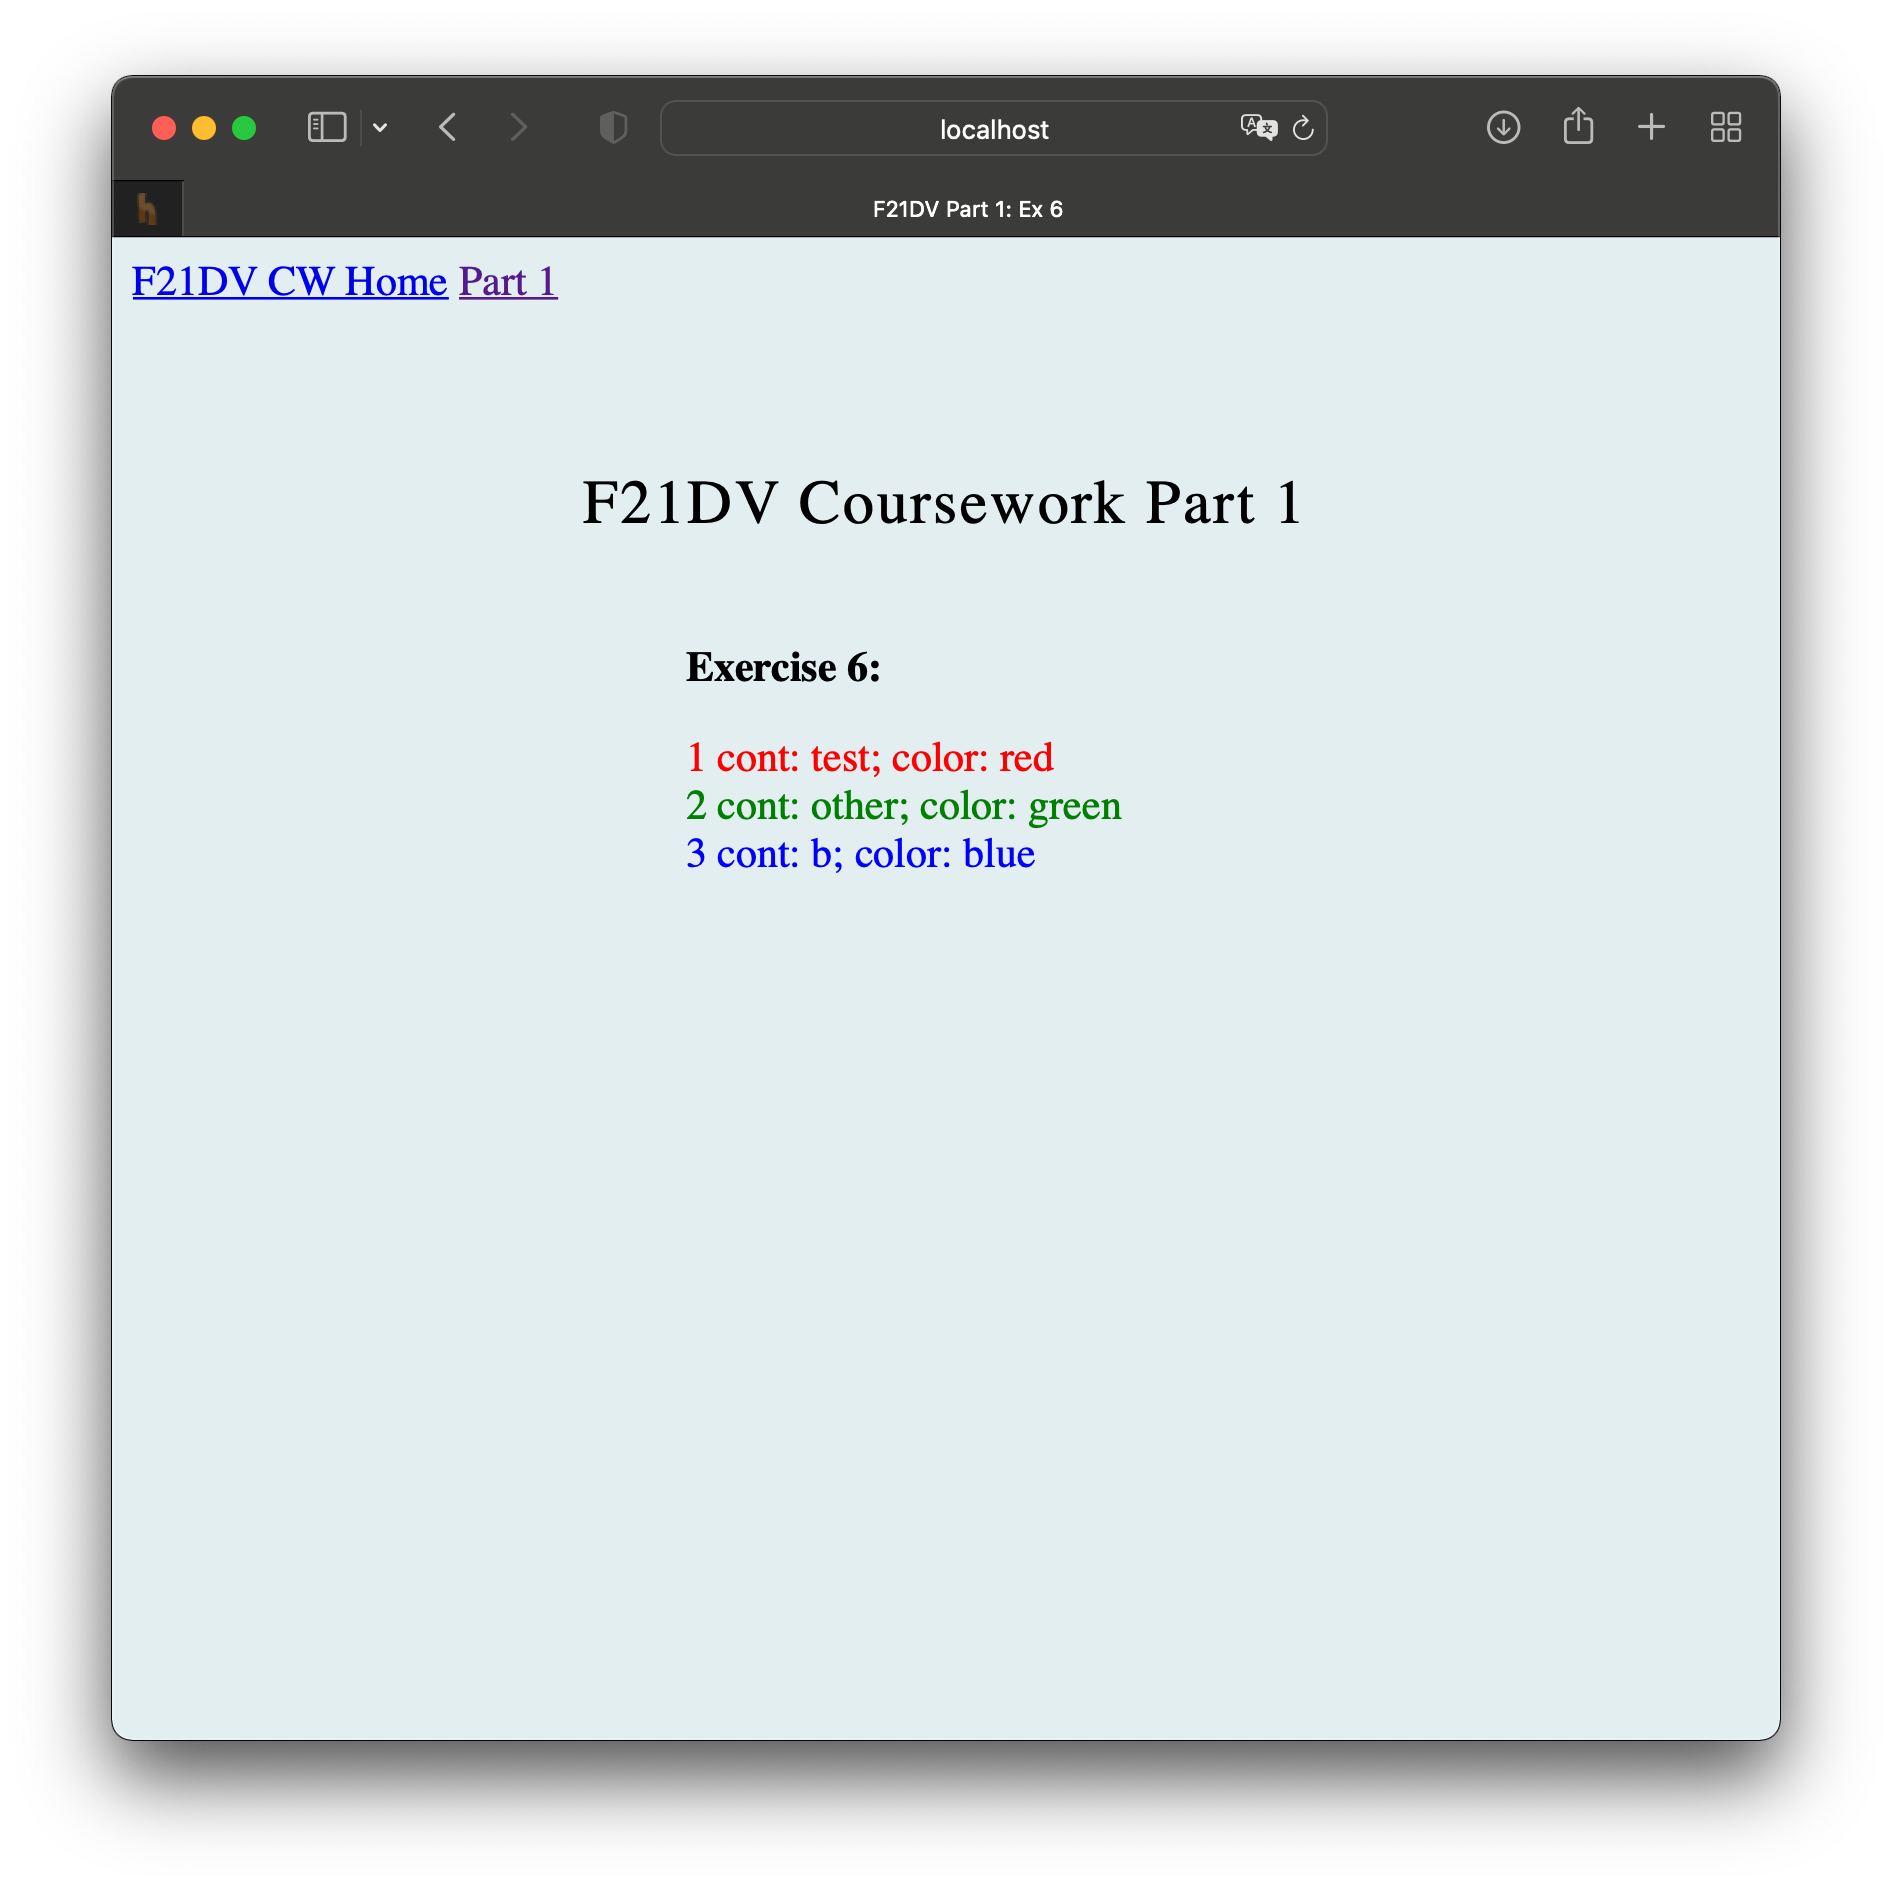
\includegraphics[width = 8cm]{images/ex6.png}
    \label{fig:ex6}
    \caption{Exercise 6}
\end{figure}
\FloatBarrier
\lstinputlisting[language=JavaScript]{../../public/js/part1/task6.js}
Exercise 6 adds an additional variable \verb|color|, and prints that out in the text field, on top of
what was originally there. I went an extra mile to style each div according to its \verb|color| value.

\newpage
\section{Exercise 7}
\begin{figure}[!ht]
    \centering
    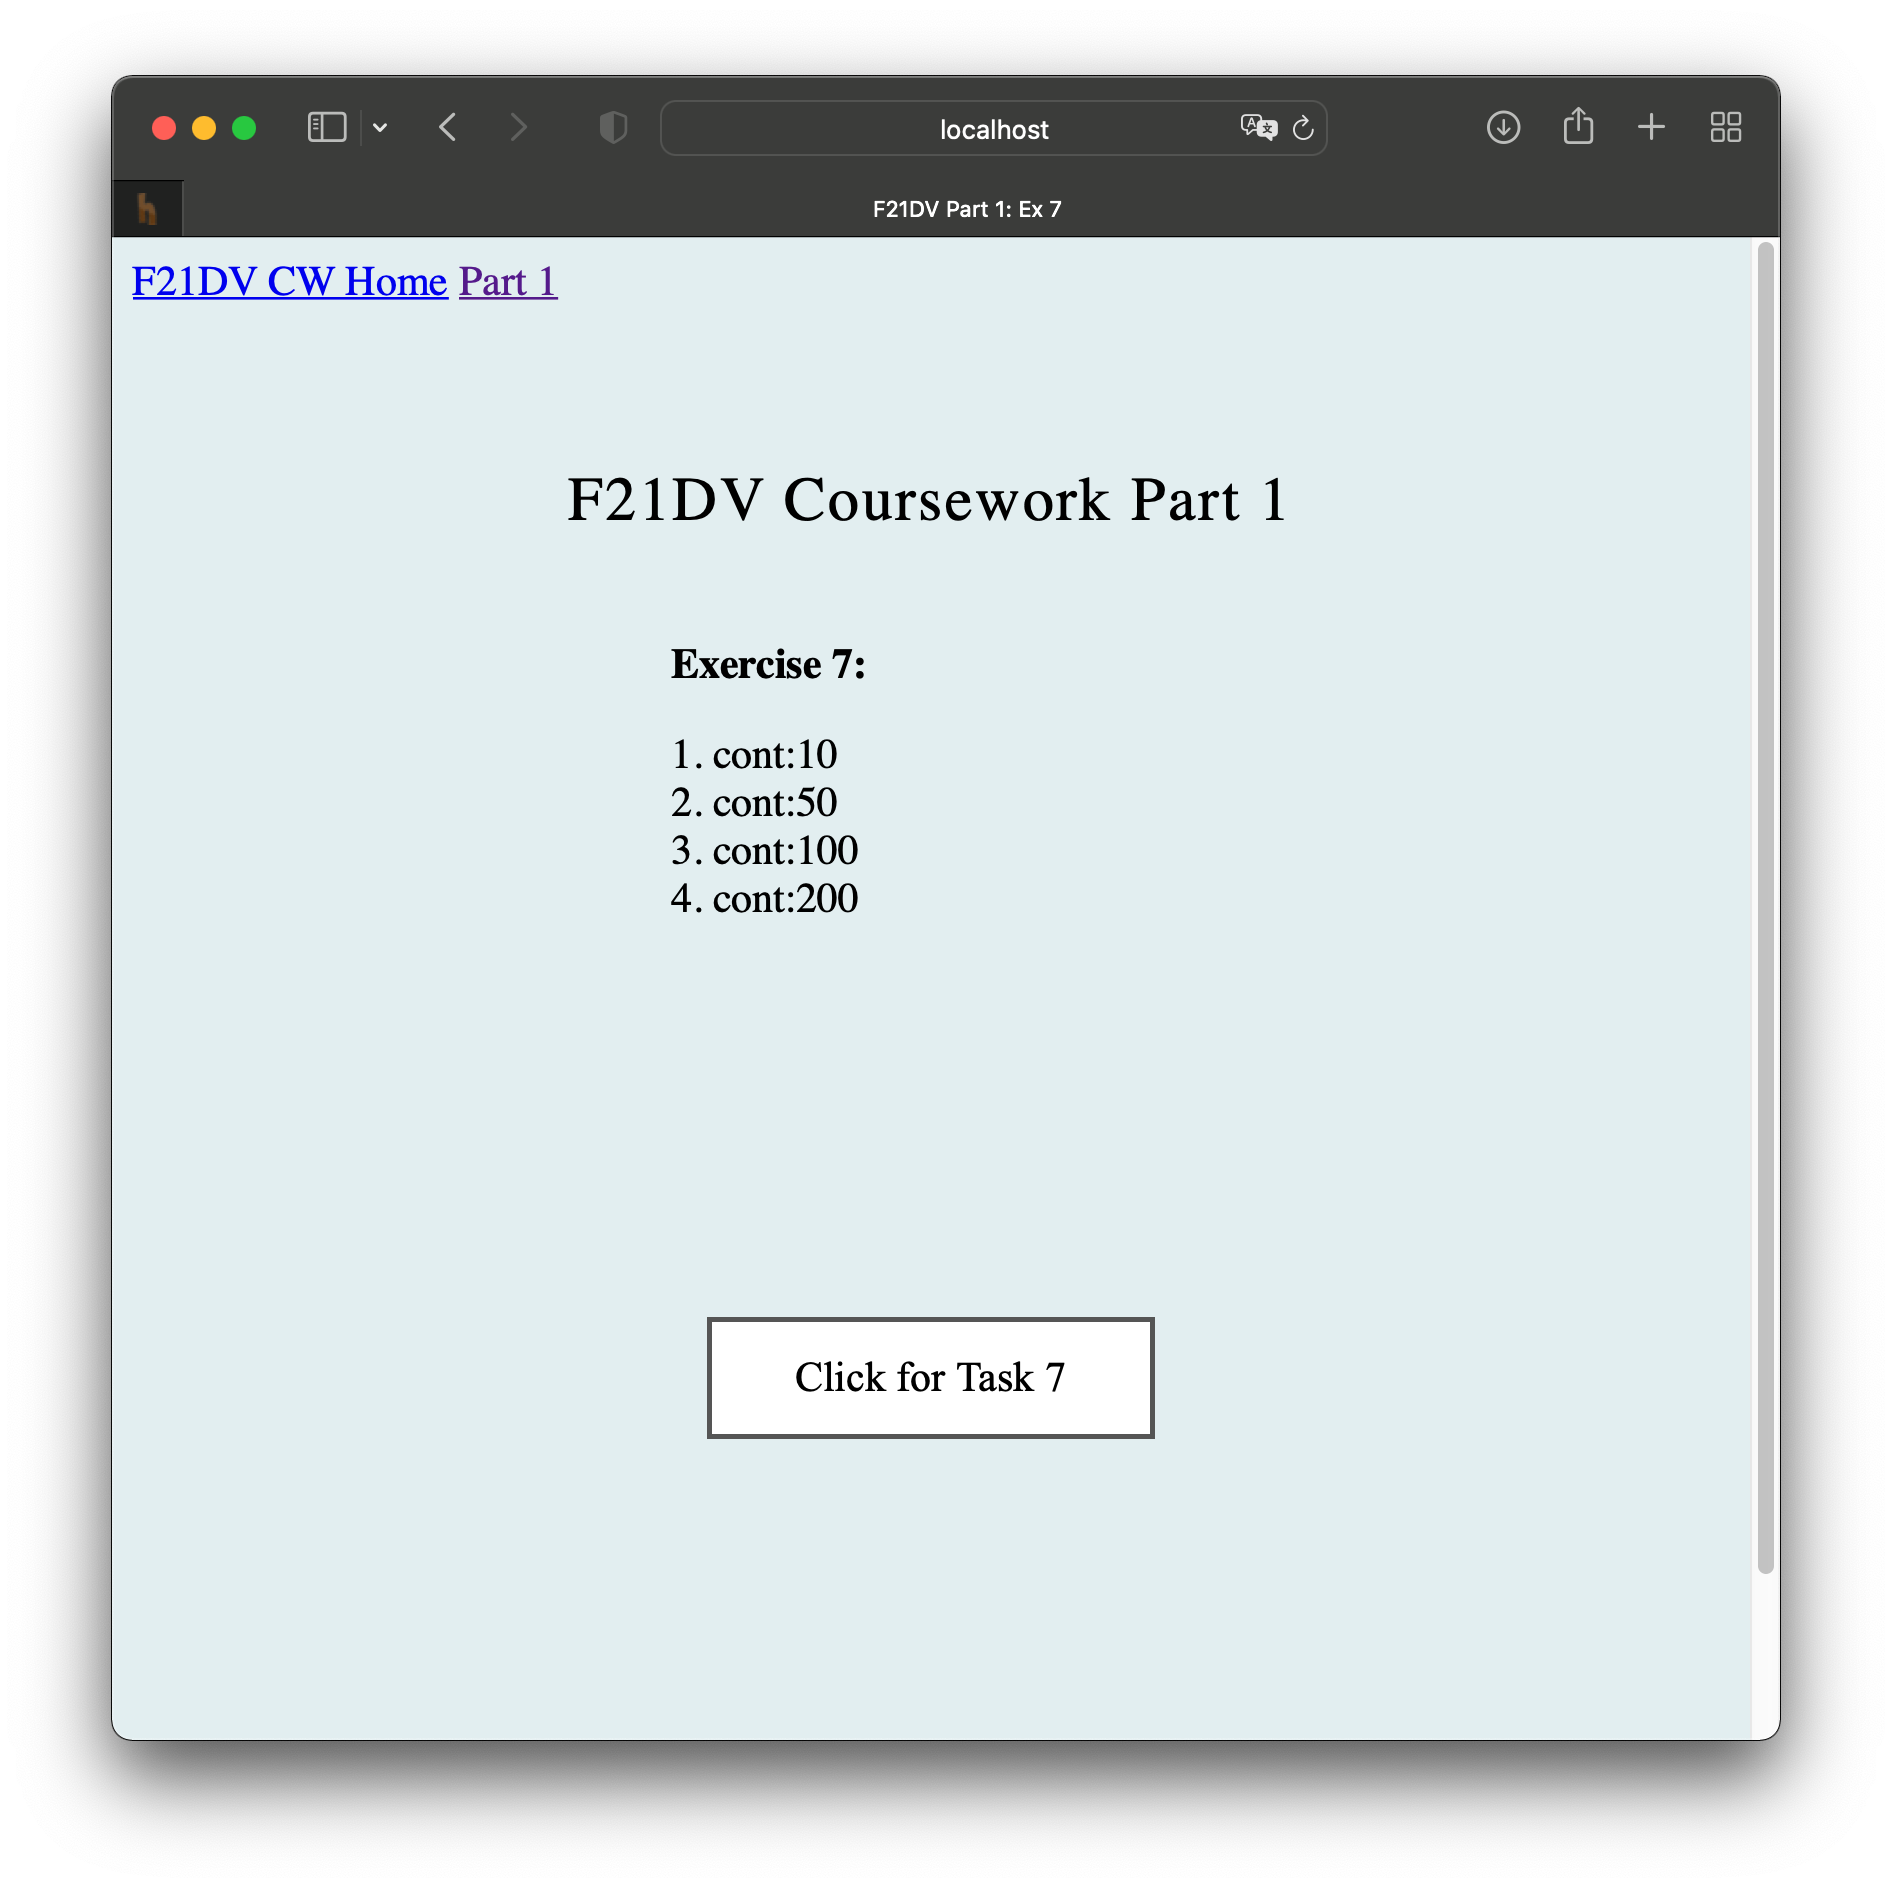
\includegraphics[width = 8cm]{images/ex7_1.png}
    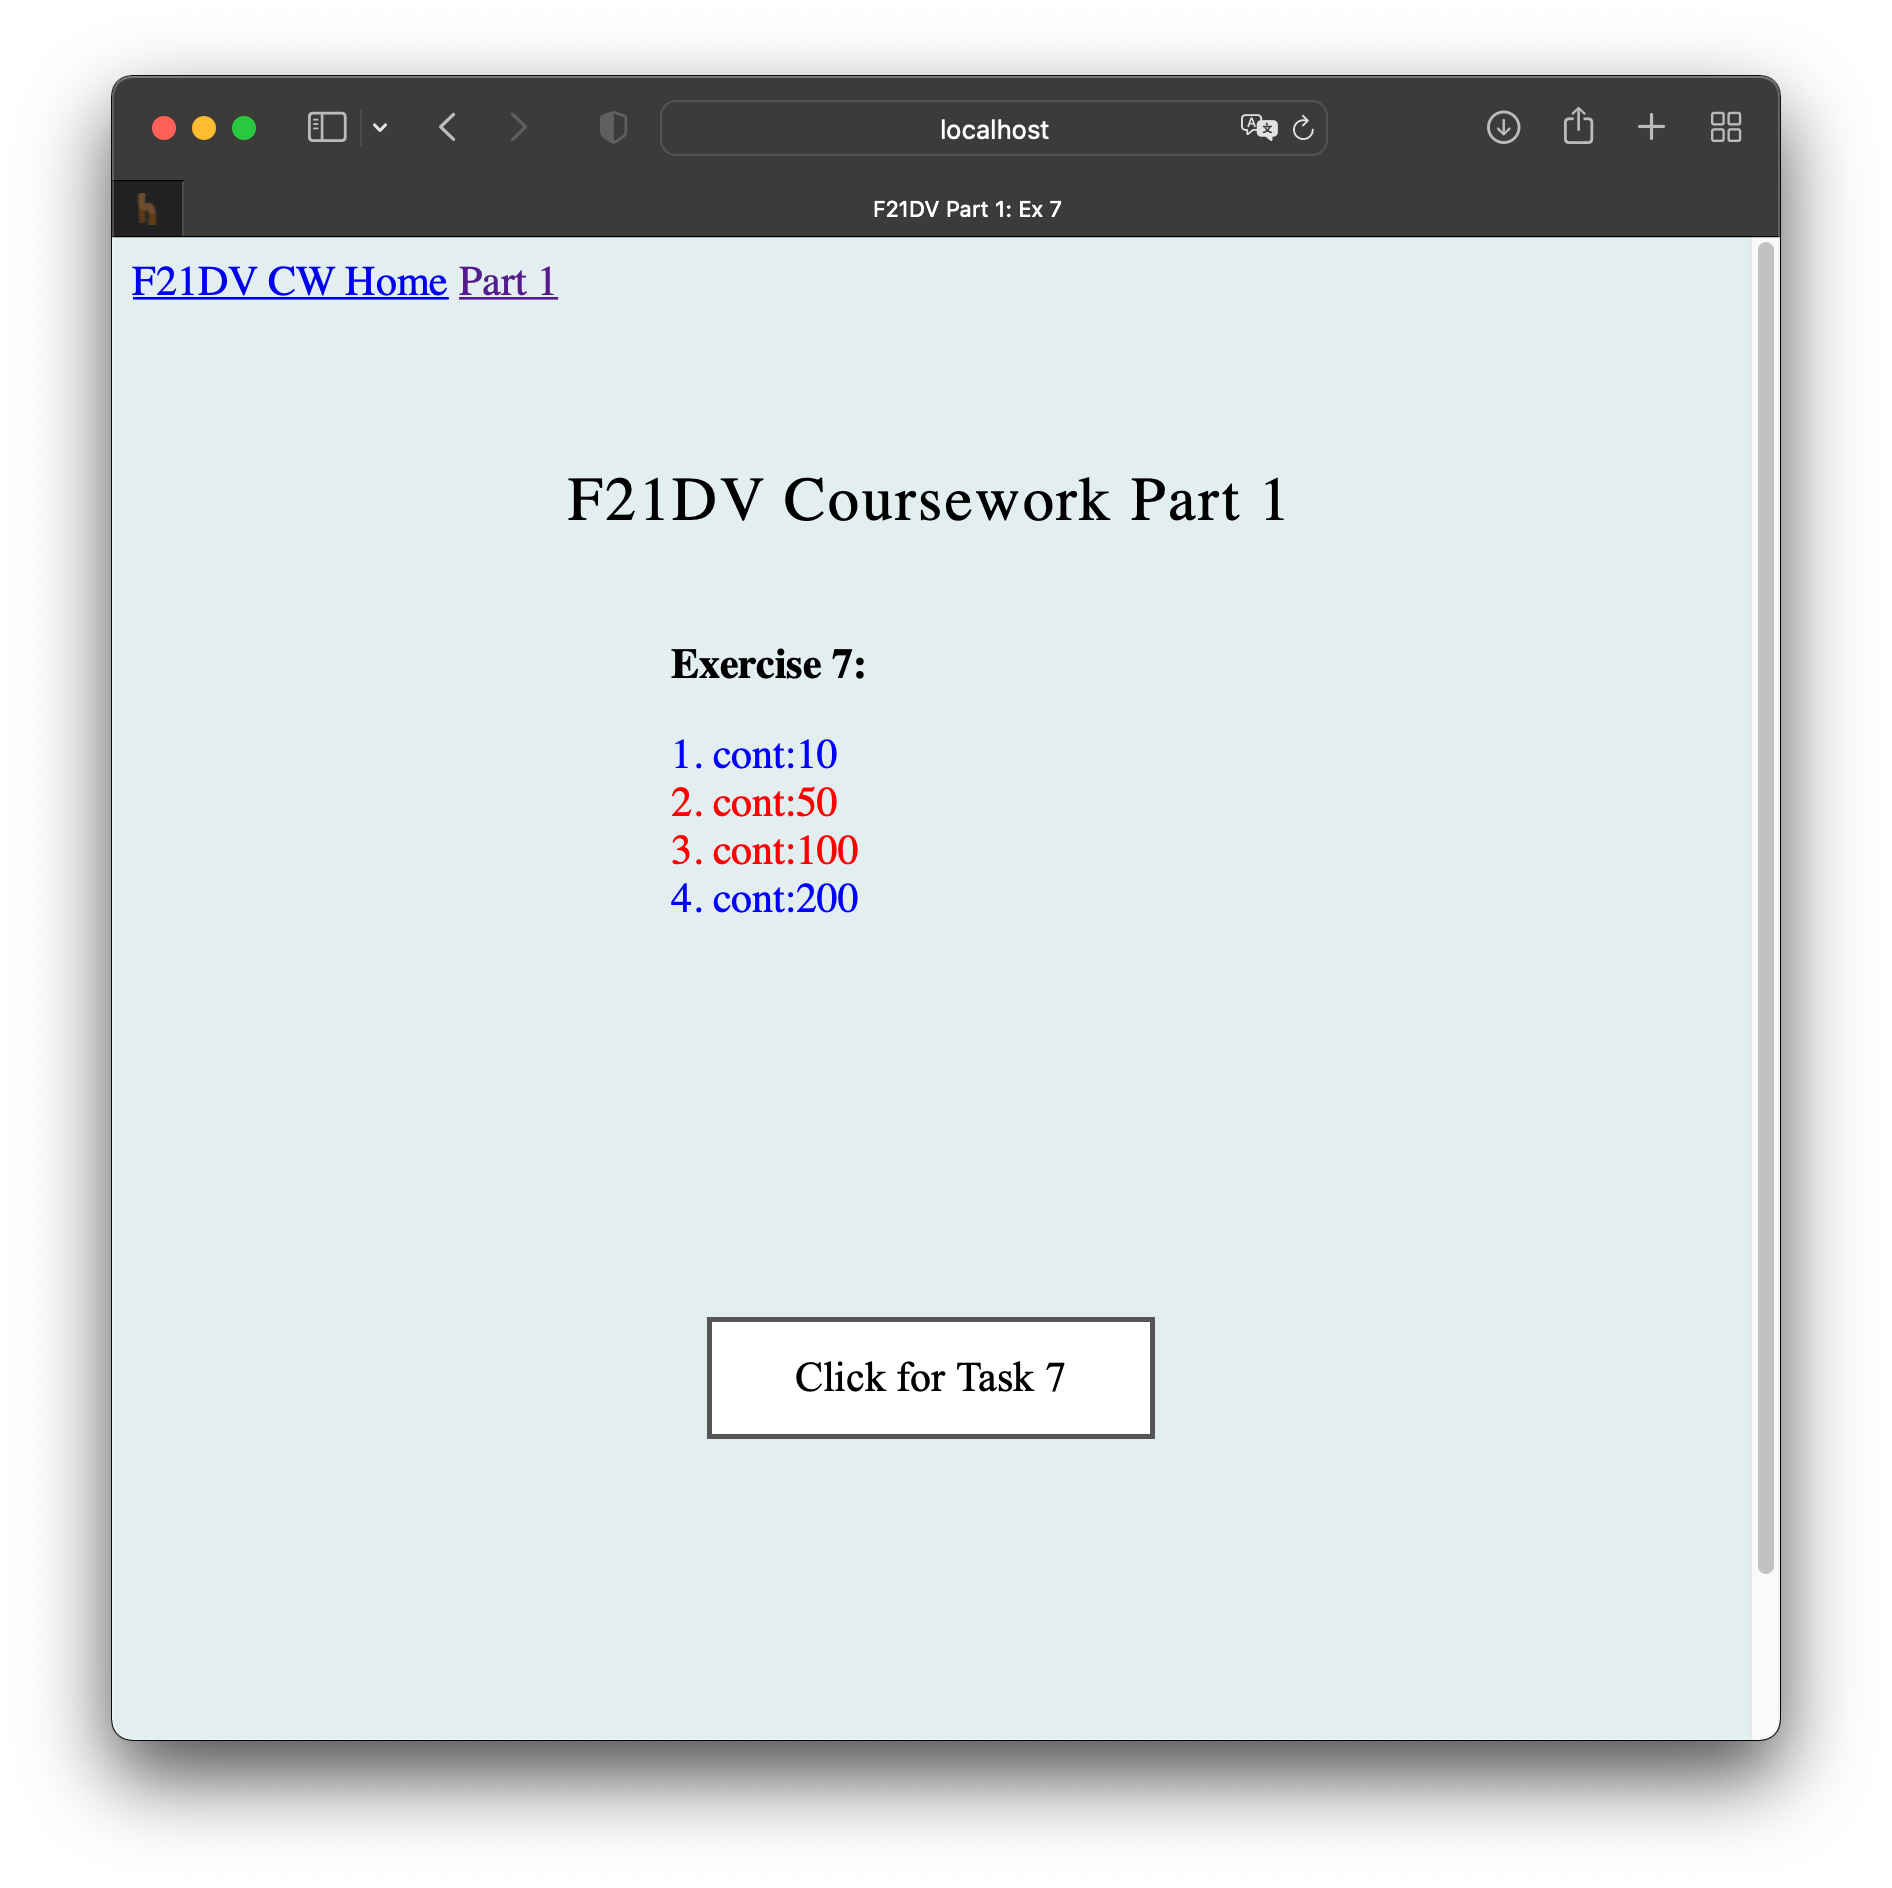
\includegraphics[width = 8cm]{images/ex7_2.png}
    \label{fig:ex7}
    \caption{Exercise 7}
\end{figure}
\FloatBarrier
% \lstinputlisting[language=JavaScript]{../../public/js/part1/task7.js}
Exercise 7 would change the colour of the div based on the values of the div. Upon click, the button
would change the div's with value of numbers between 50 and 100 to red, and the remaining ones to blue.
Upon clicking again, the button would revert the state of the divs to their original ones. 

\newpage
\section{Exercise 8}
\begin{figure}[!ht]
    \centering
    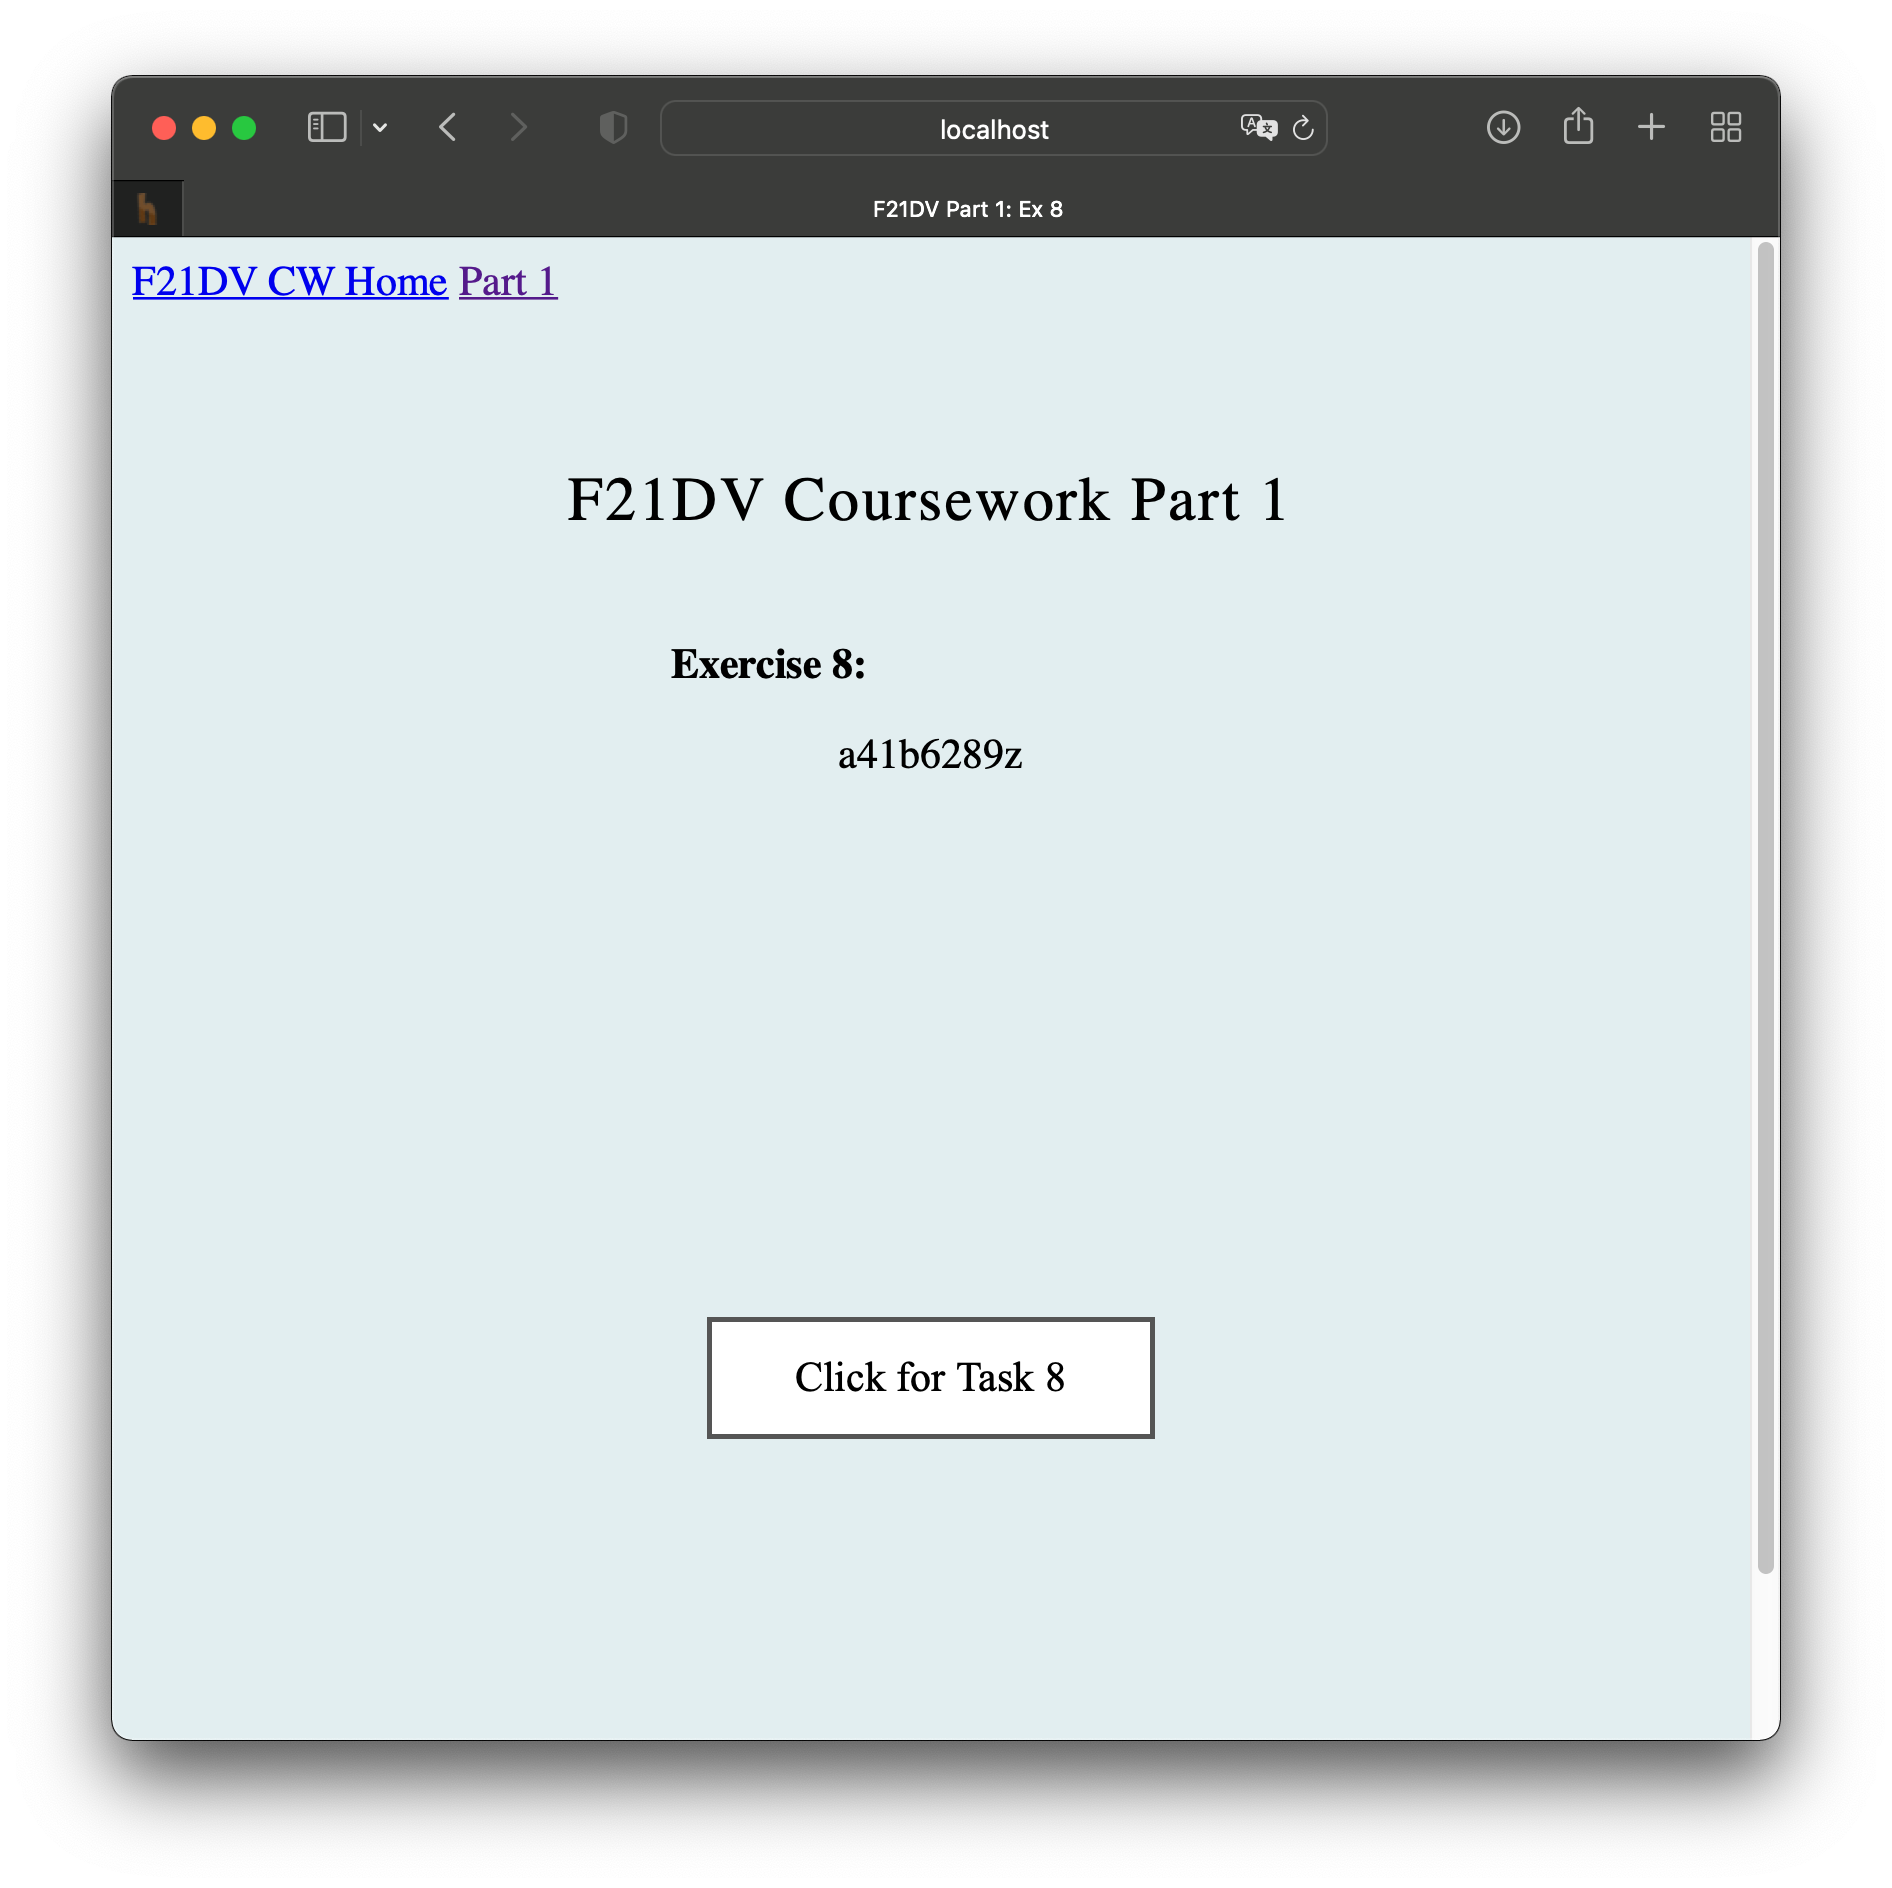
\includegraphics[width = 8cm]{images/ex8_1.png}
    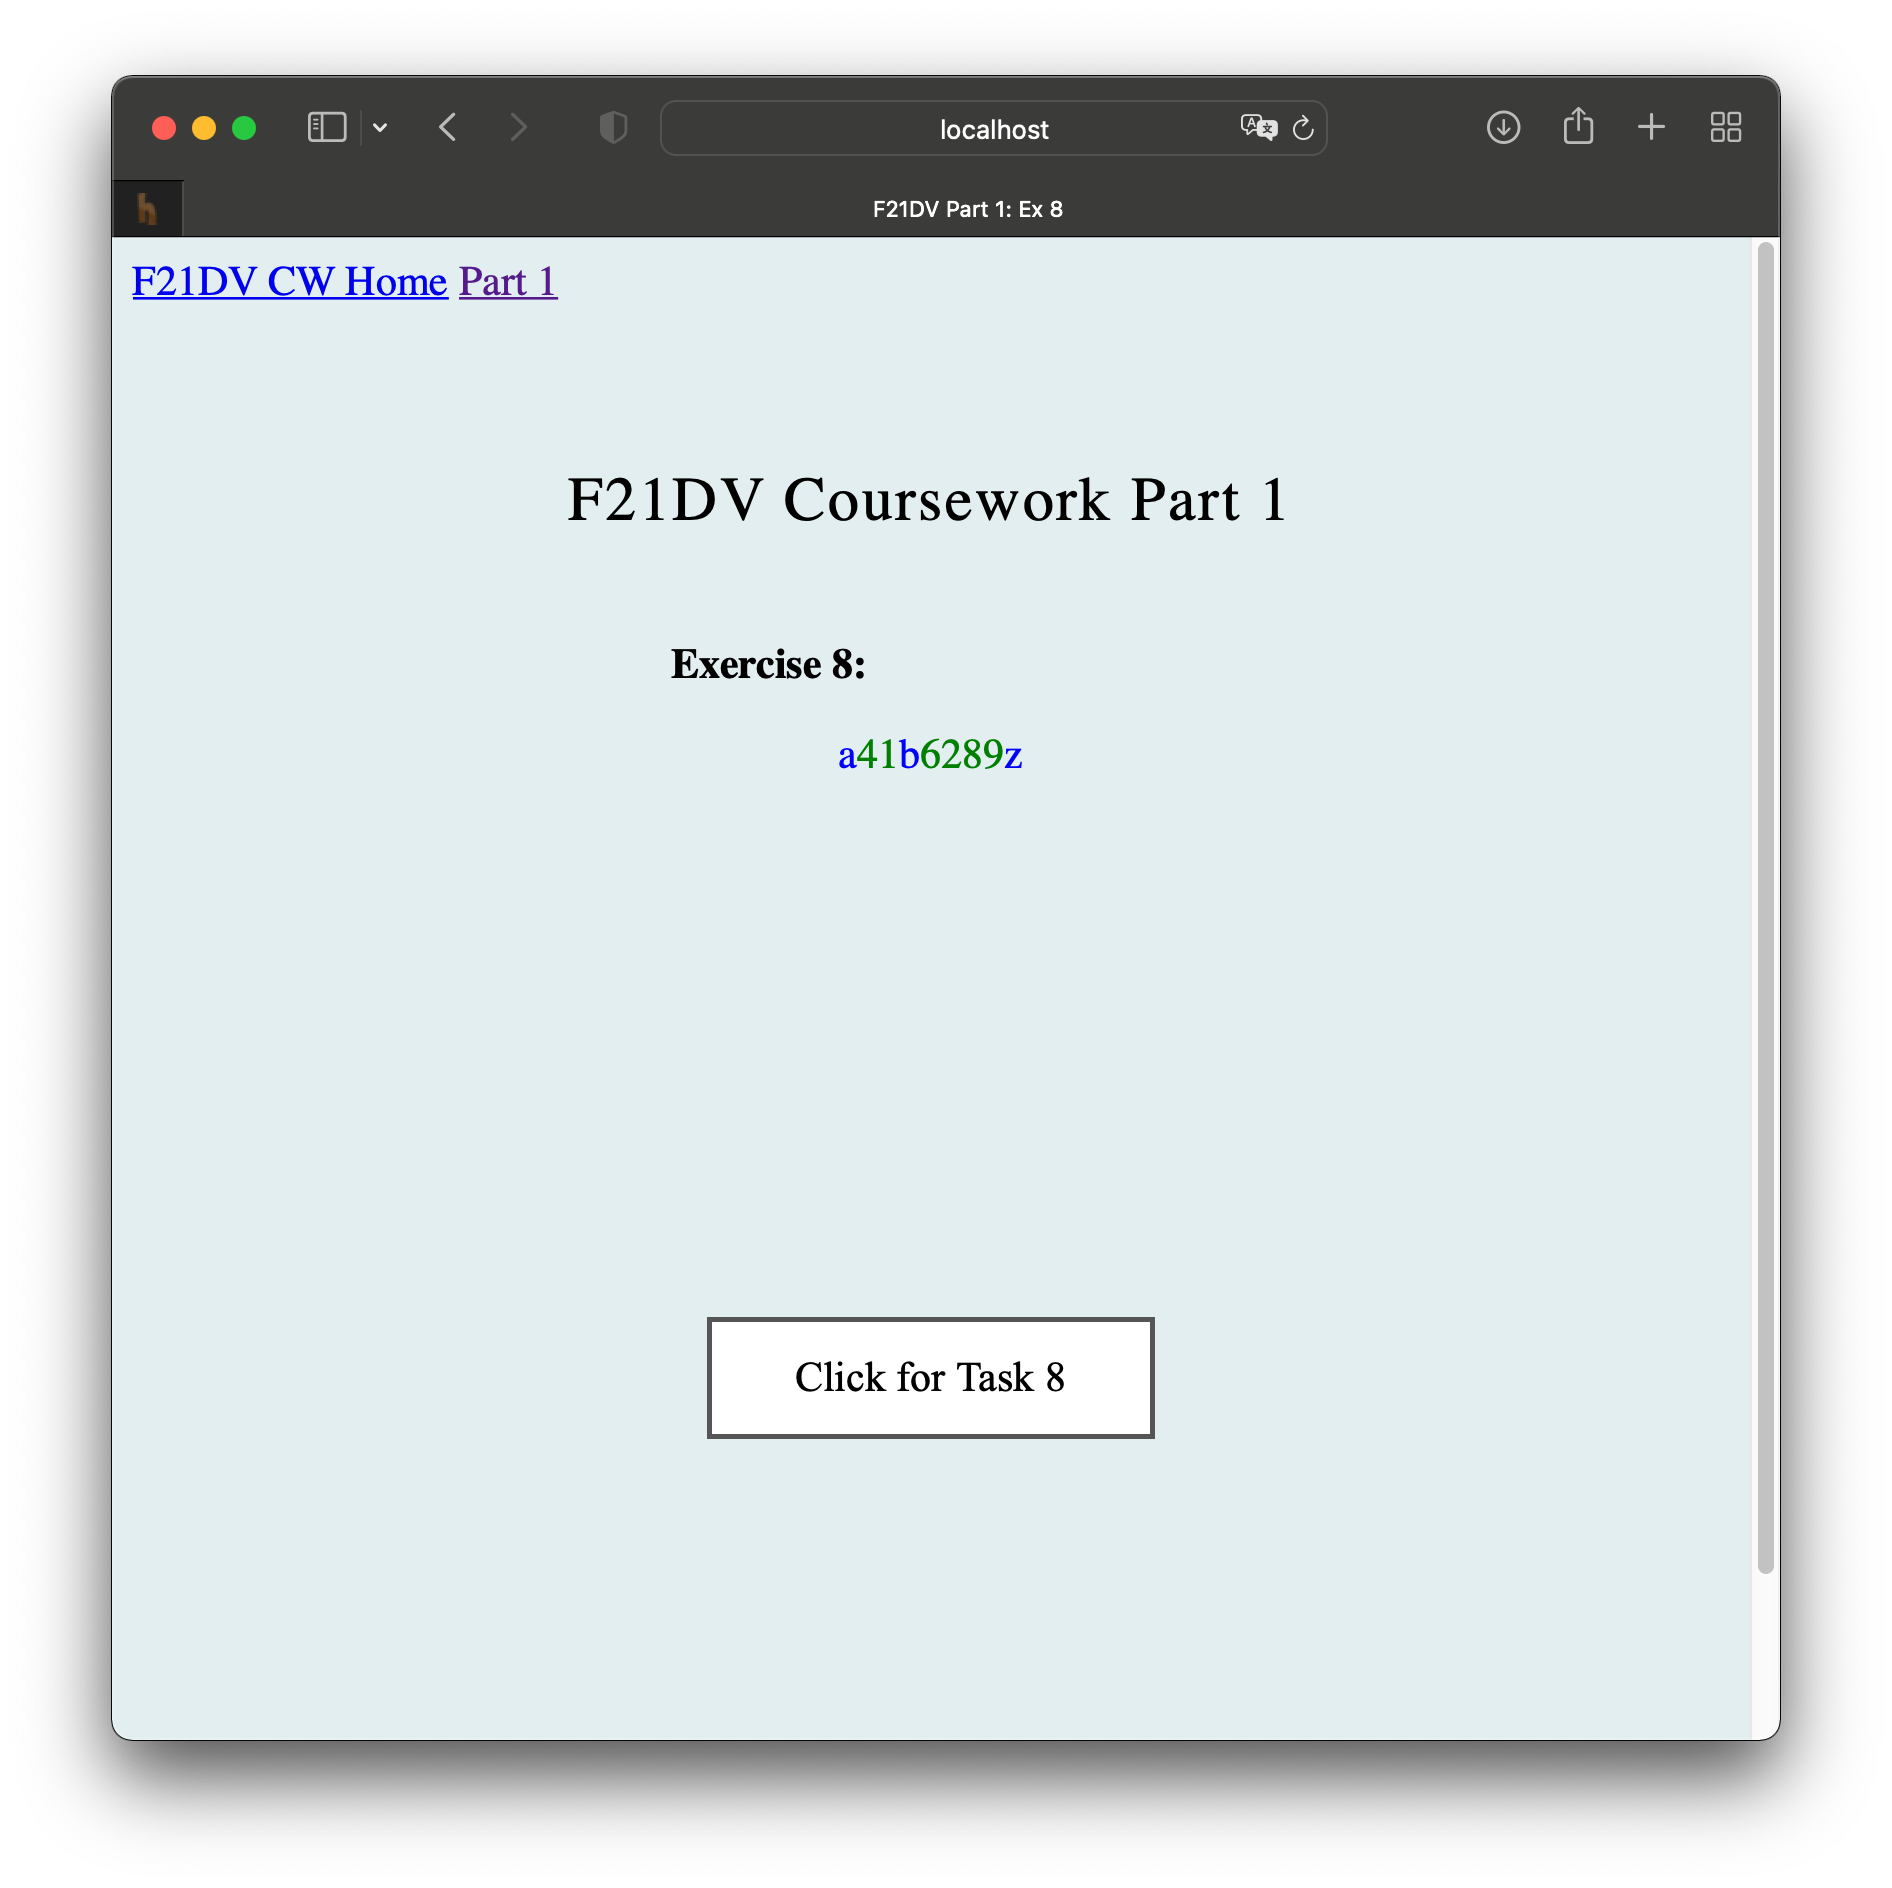
\includegraphics[width = 8cm]{images/ex8_2.png}
    \label{fig:ex8}
    \caption{Exercise 8}
\end{figure}
\FloatBarrier
% \lstinputlisting[language=JavaScript]{../../public/js/part1/task8.js}
Exercise 8's goal is to set the text colour of a string made out of the \verb|span|s, where if a
character is a number, its colour is green, and if its an alphabet, its colour is blue.

\newpage
\section{Exercise 9}
\begin{figure}[!ht]
    \centering
    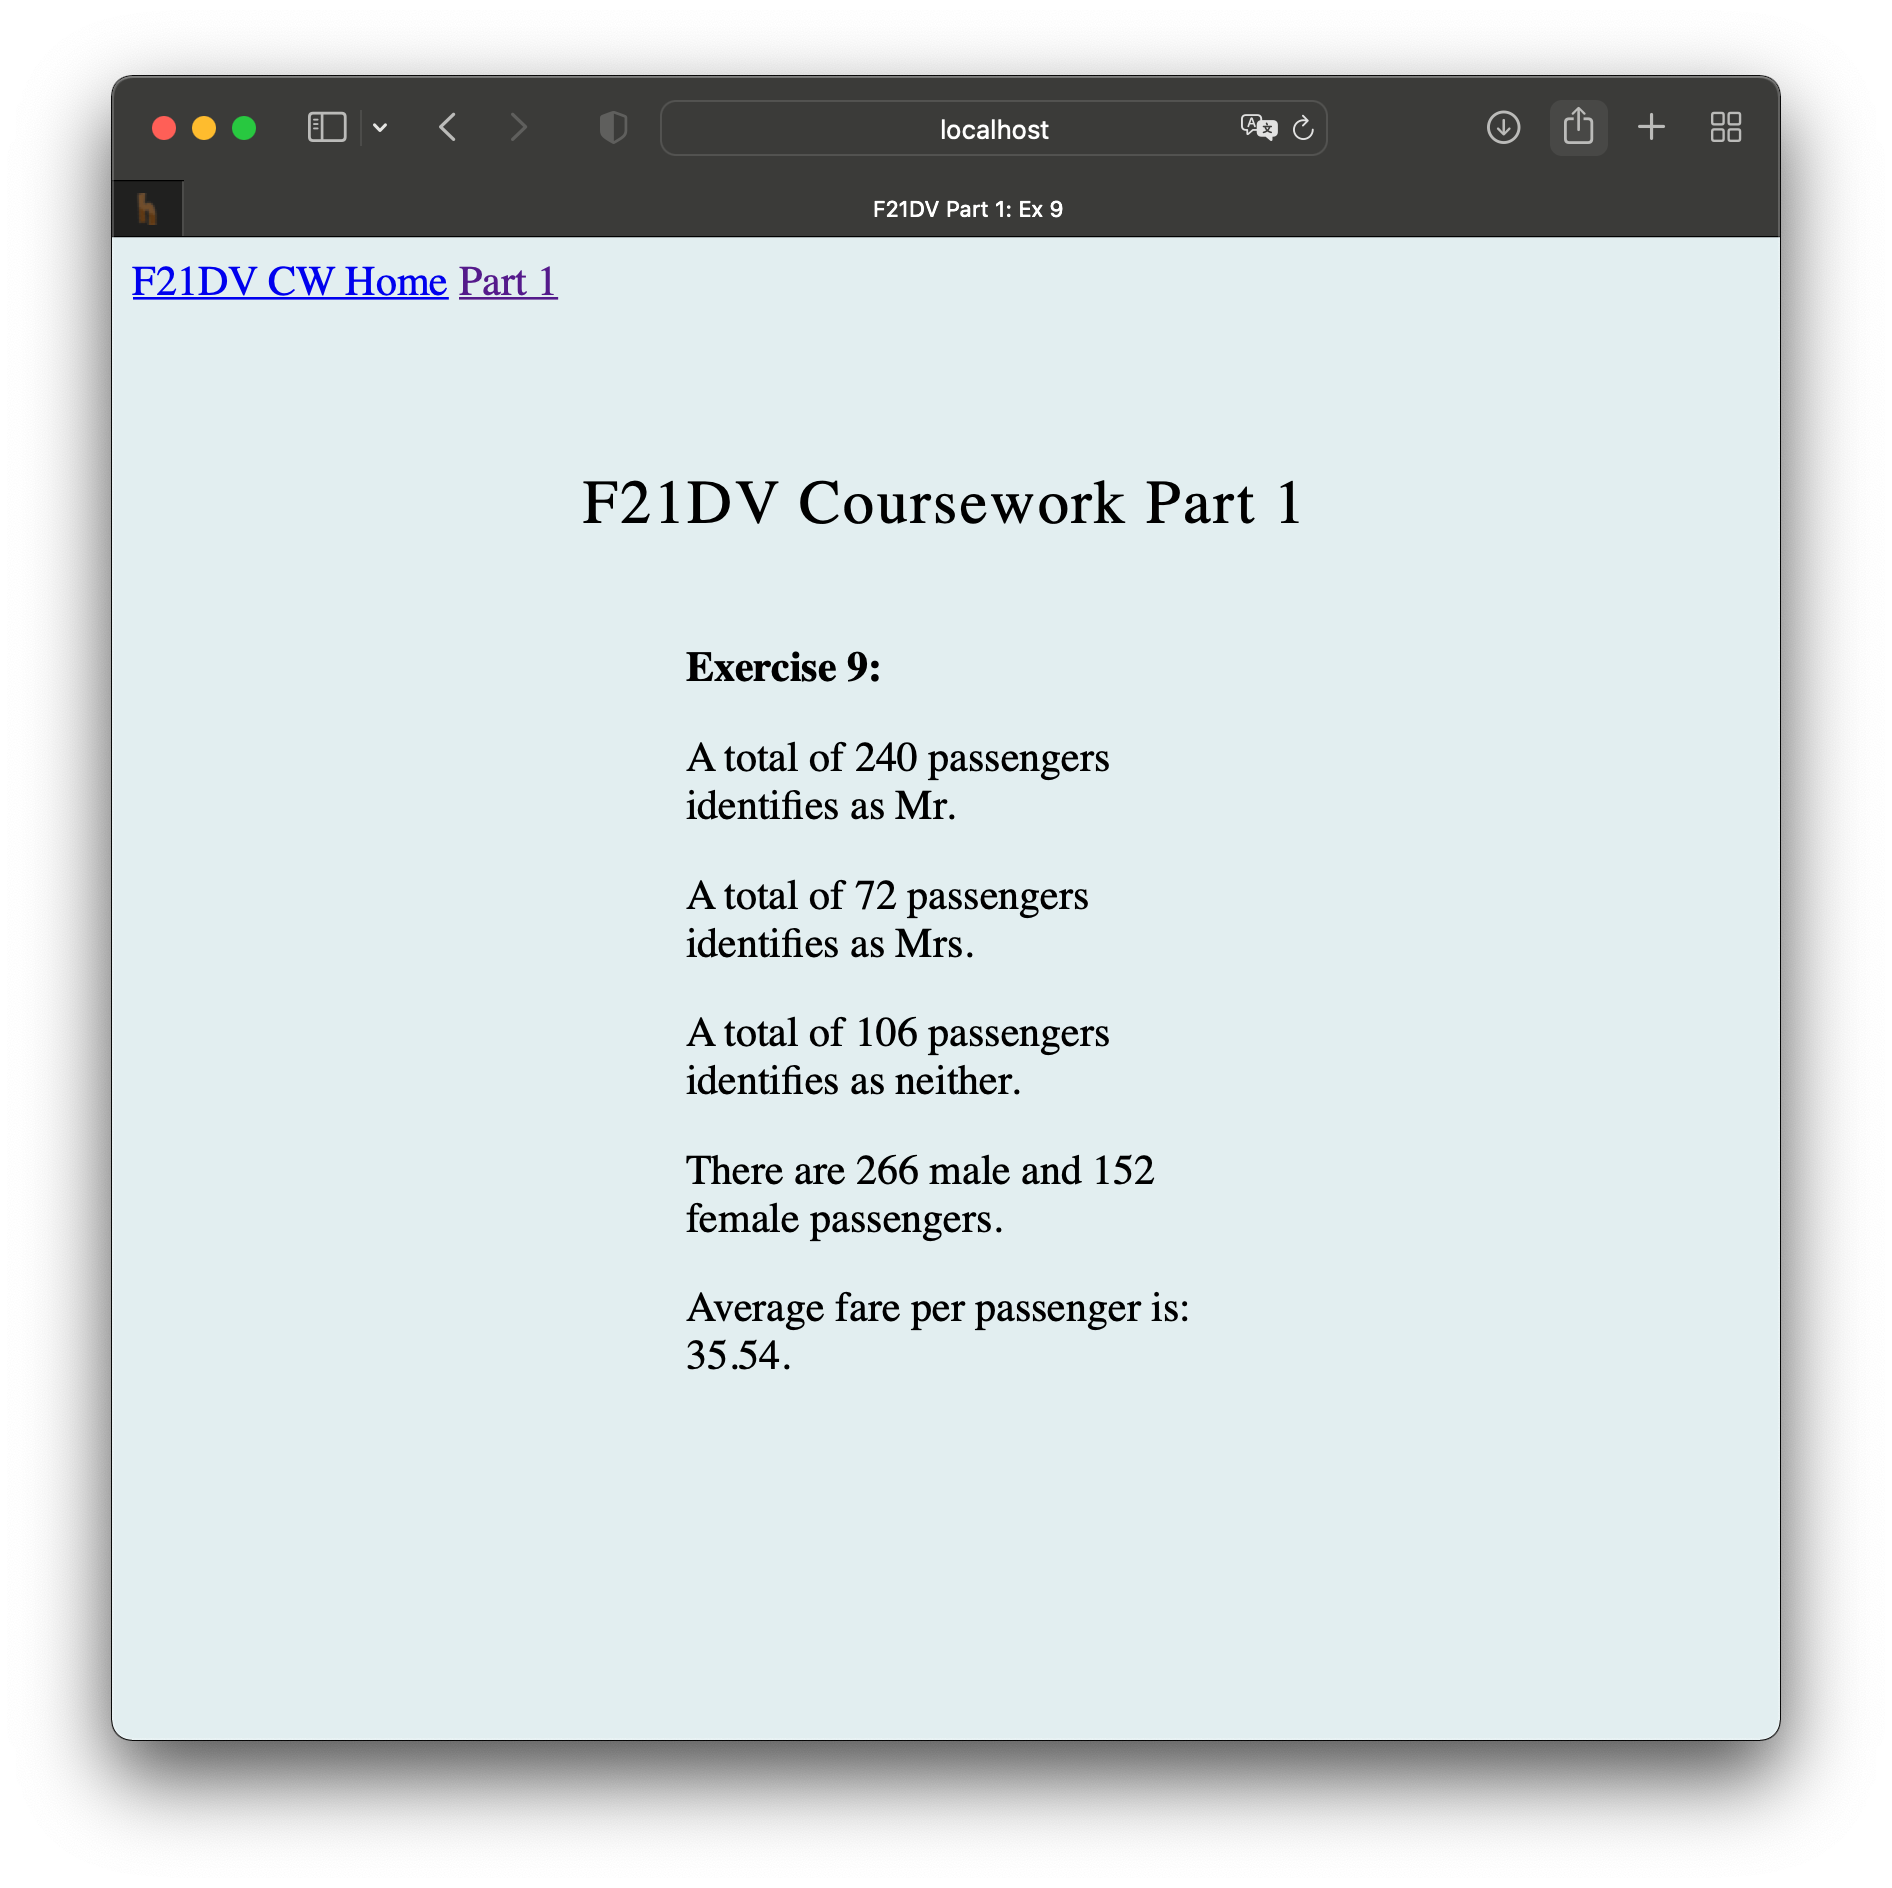
\includegraphics[width = 10cm]{images/ex9.png}
    \label{fig:ex9}
    \caption{Exercise 9}
\end{figure}
\FloatBarrier
\lstinputlisting[language=JavaScript]{../../public/js/part1/task9.js}
Exercise 9 reads in the csv data, then processes it to count the number of passengers with a Mr. or 
Mrs. title, and also counts the number of male/female passengers. I have also added on a calculation that
calculates the average fare price per titanic passenger. This was done by adding all non-NaNs to a local
variable, then dividing it by total passenger. 

\newpage
\section{Exercise 10}
\begin{figure}[!ht]
    \centering
    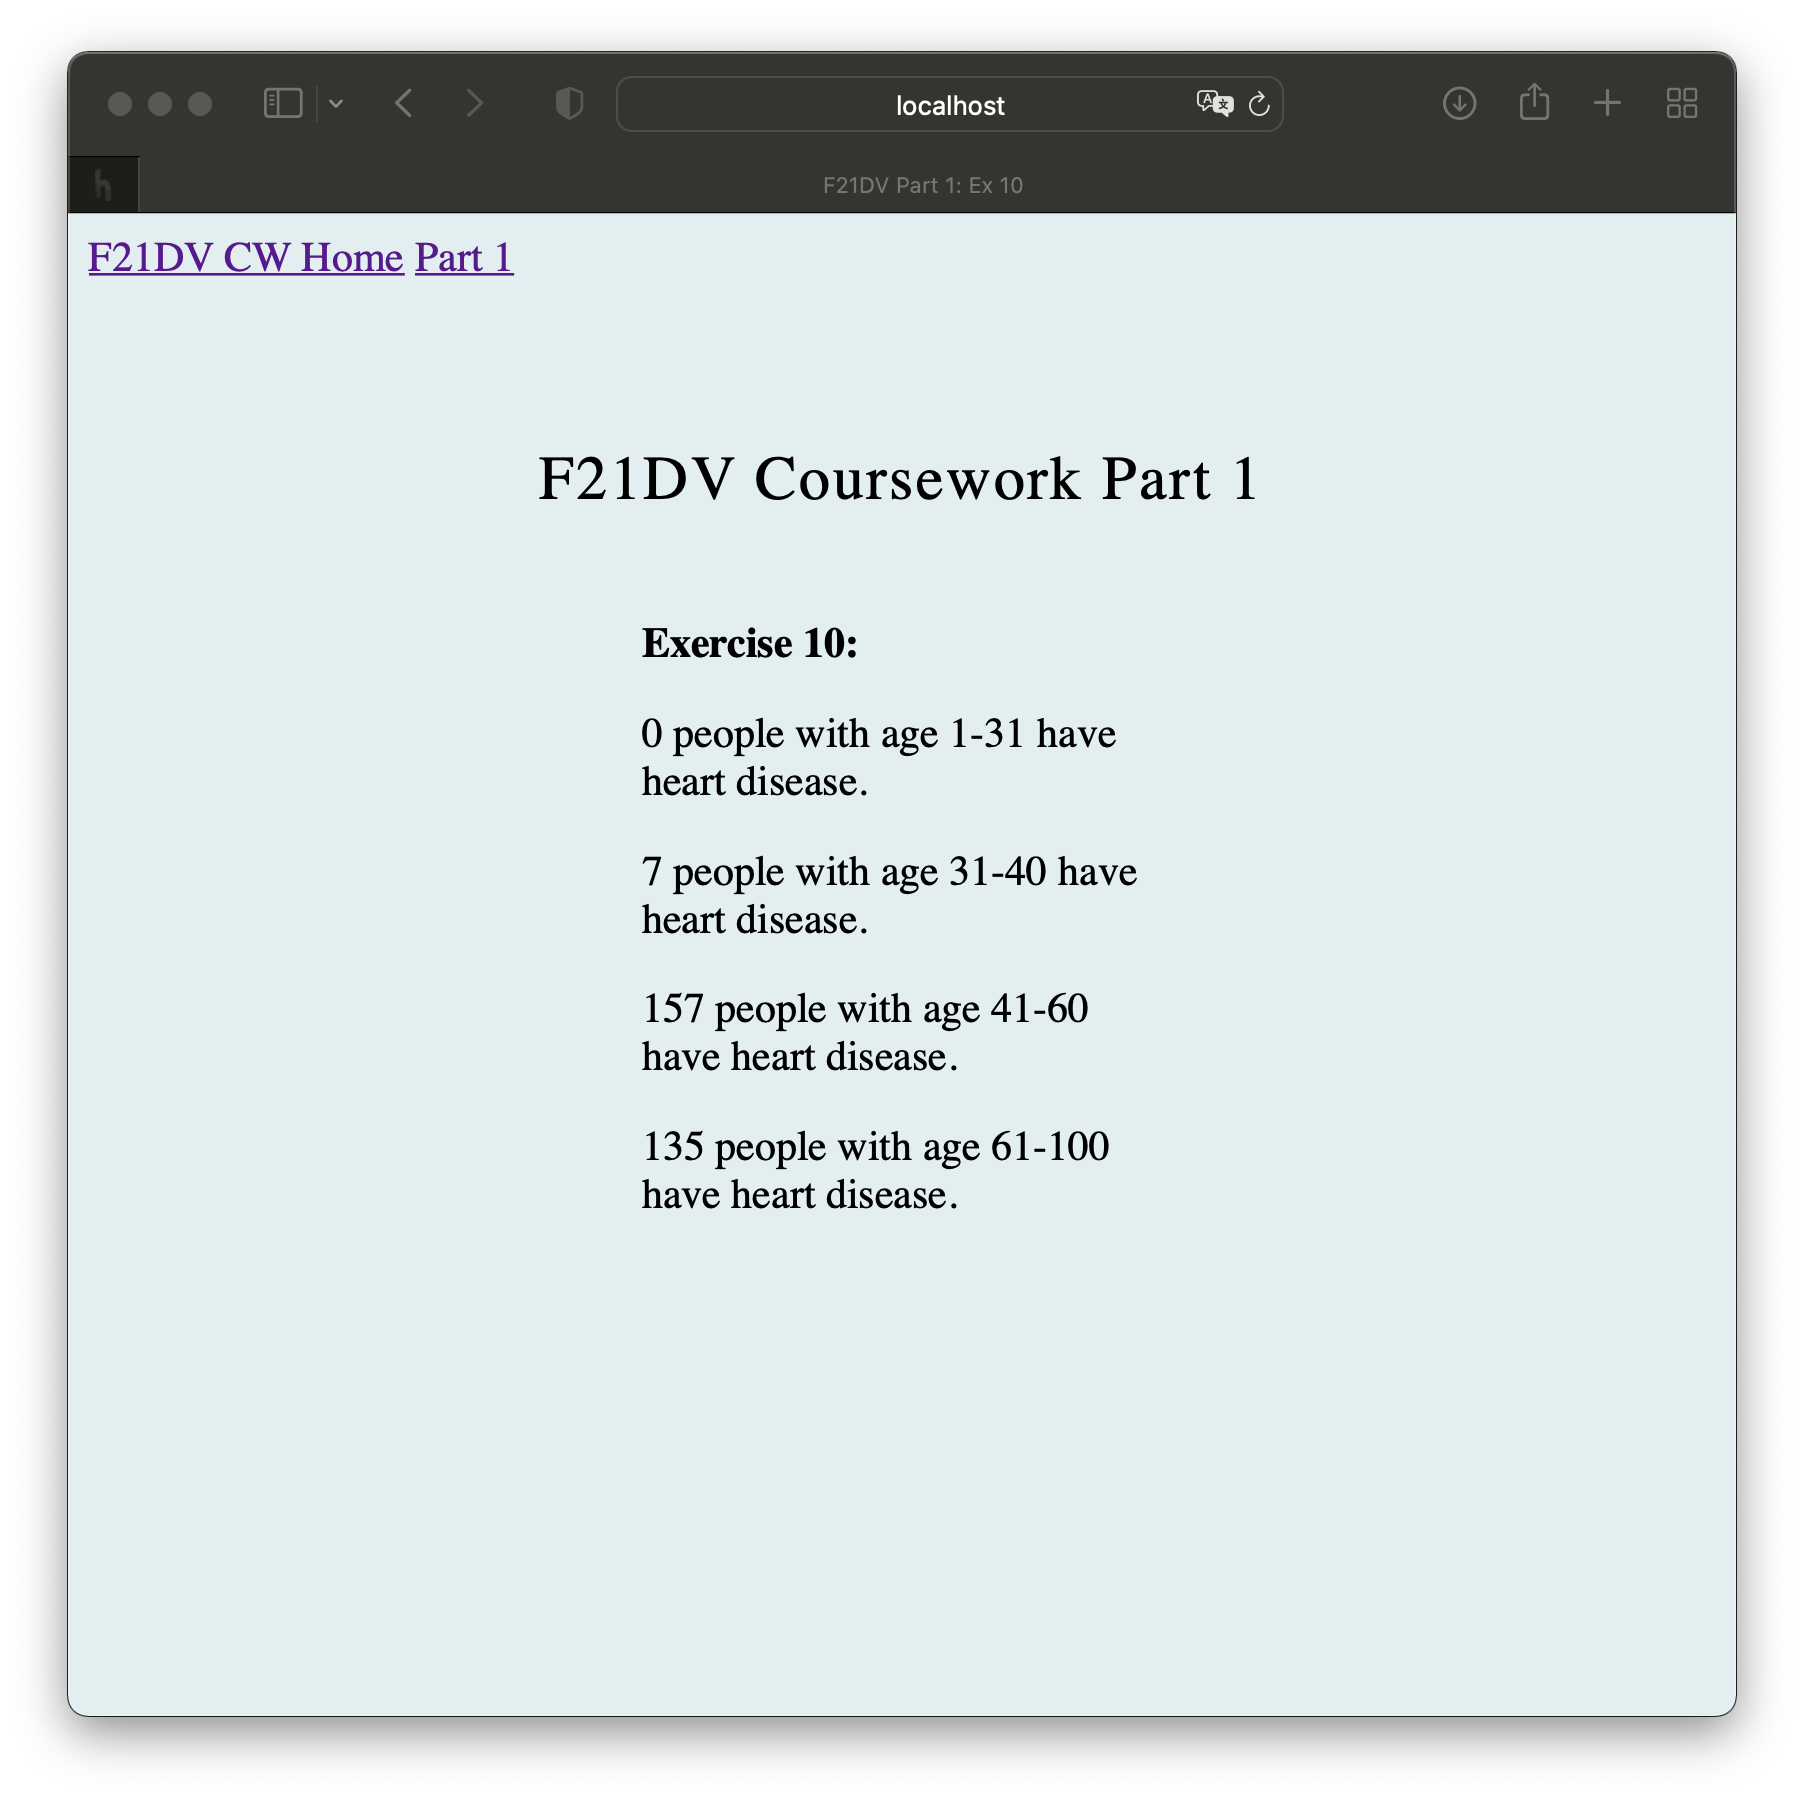
\includegraphics[width = 10cm]{images/ex10.png}
    \label{fig:ex10}
    \caption{Exercise 10}
\end{figure}
\FloatBarrier
\lstinputlisting[language=JavaScript]{../../public/js/part1/task10.js}
Exercise 10 is pretty much the same as exercise 9. Calling the right variable \verb|name| and then processing
its values. However, since the heart data is being used again at a later exercise, I have created an async
function that exports the data, so that the process is only done once. 

\newpage
\section{Exercise 11}
\begin{figure}[!ht]
    \centering
    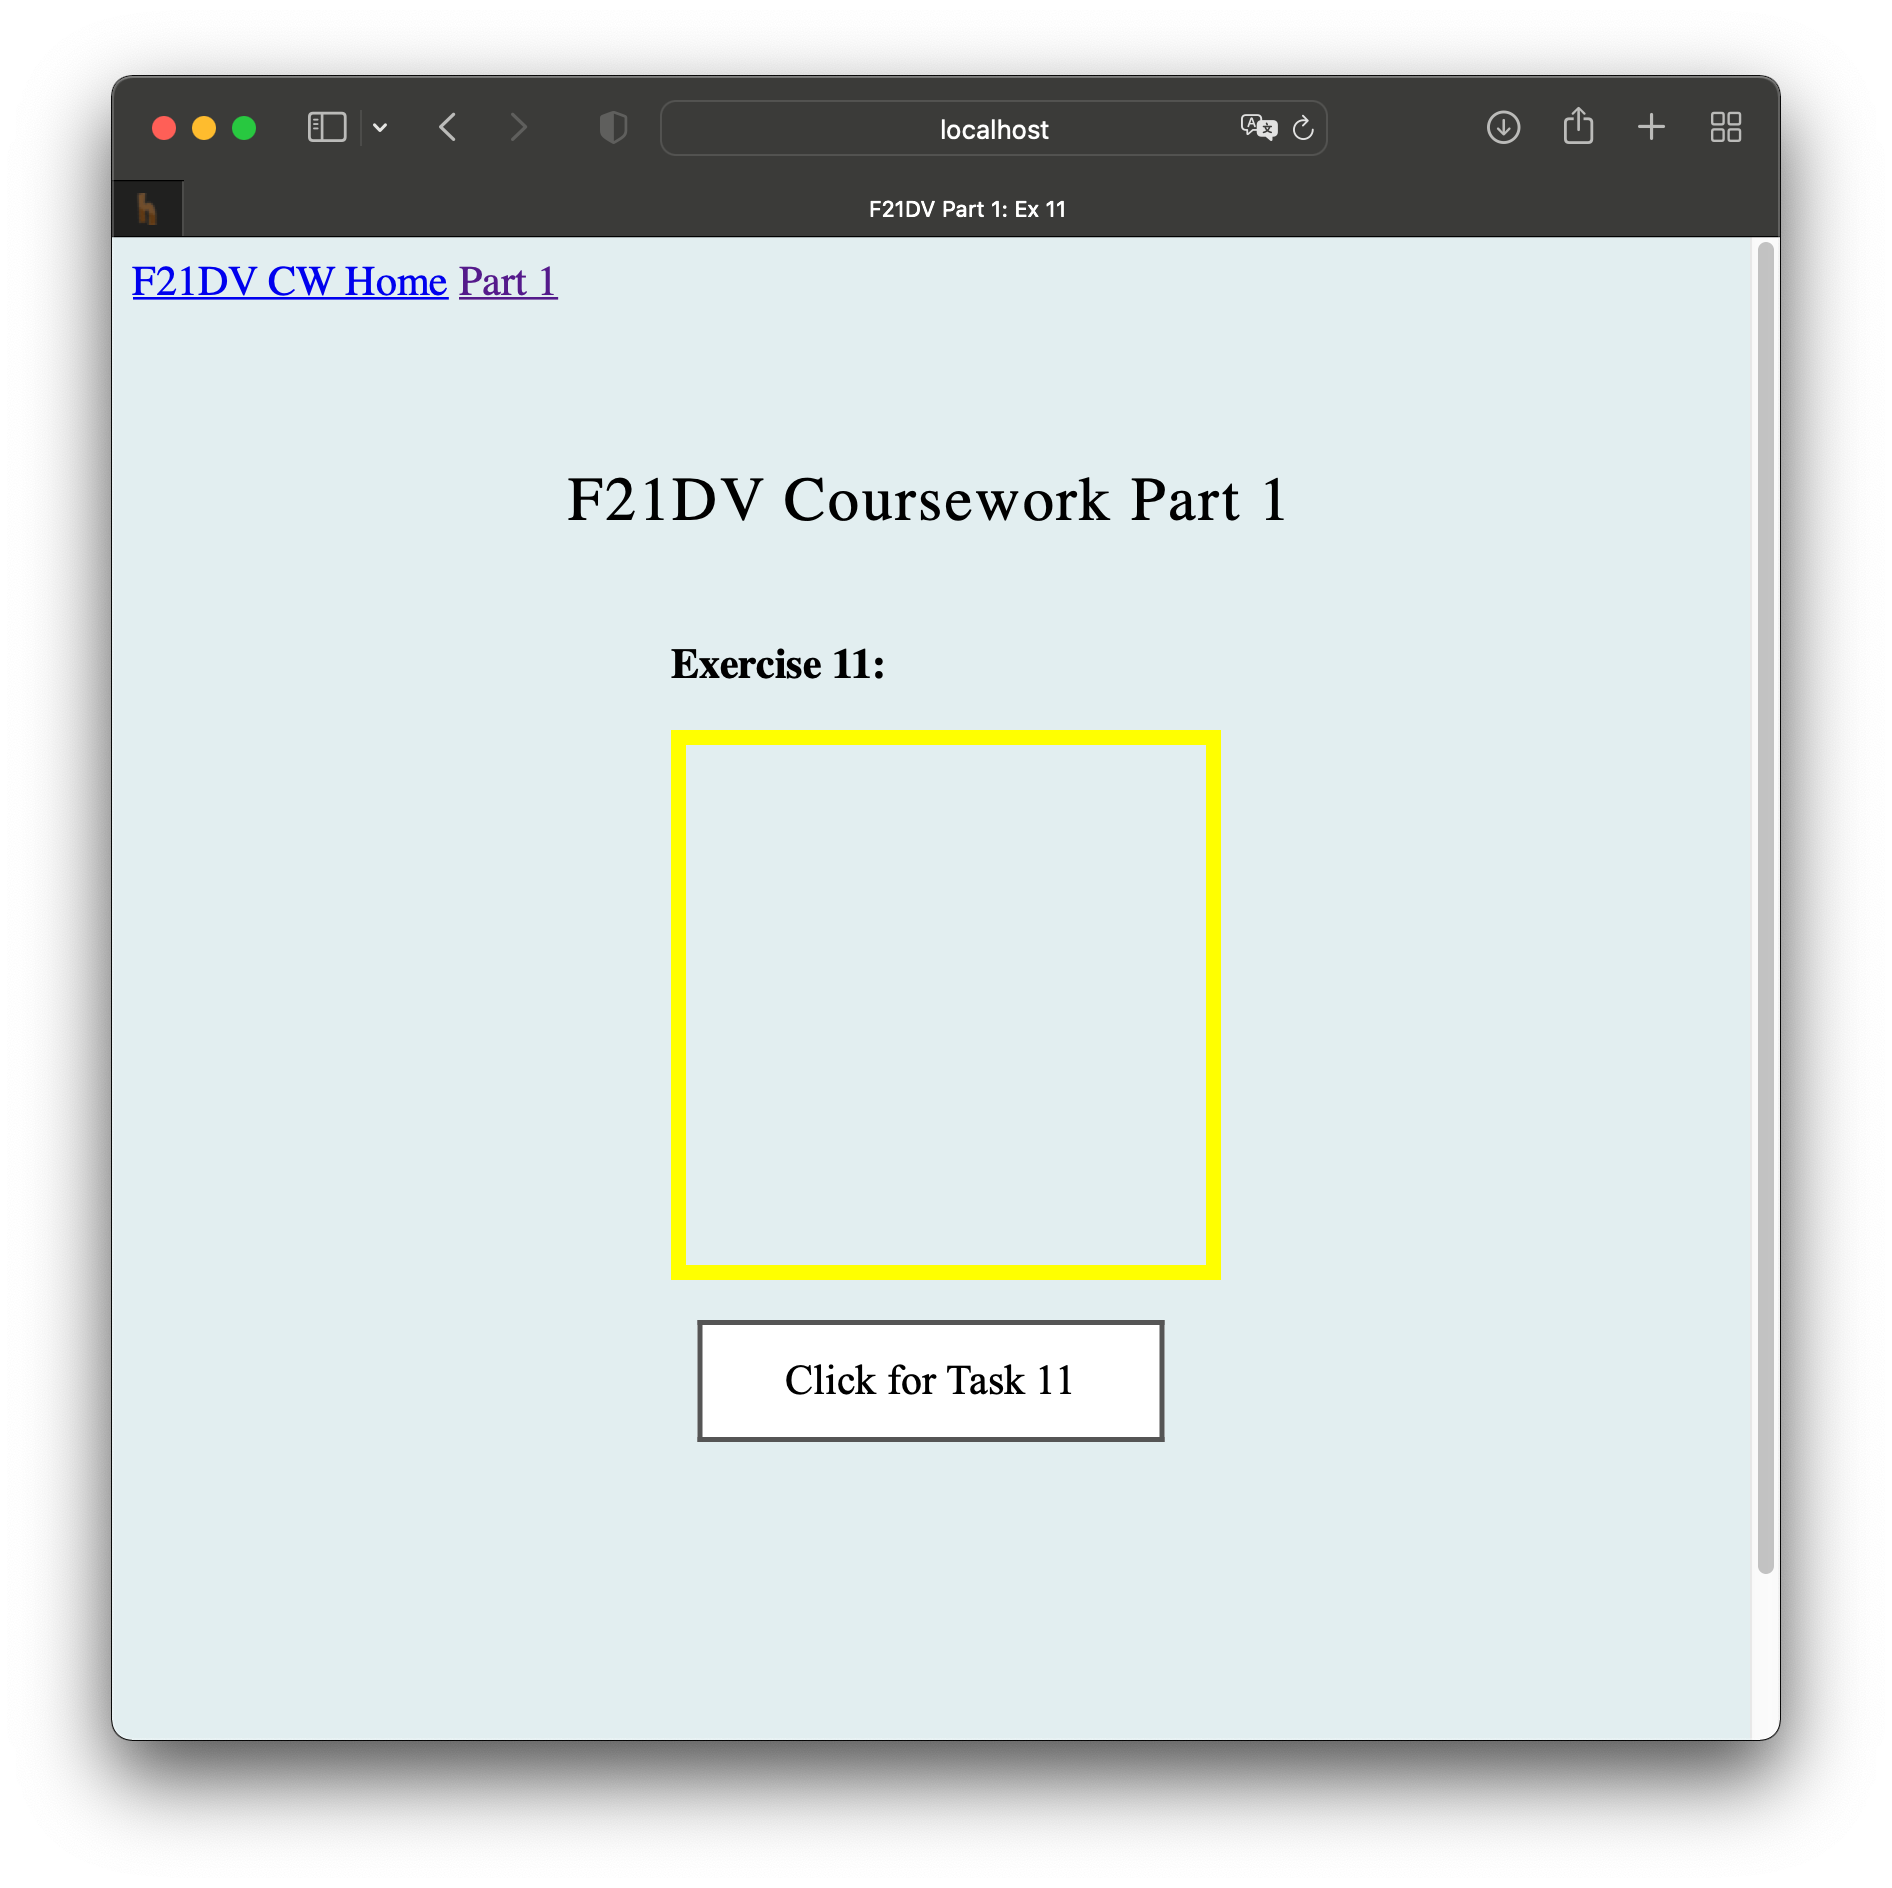
\includegraphics[width = 8cm]{images/ex11_1.png}
    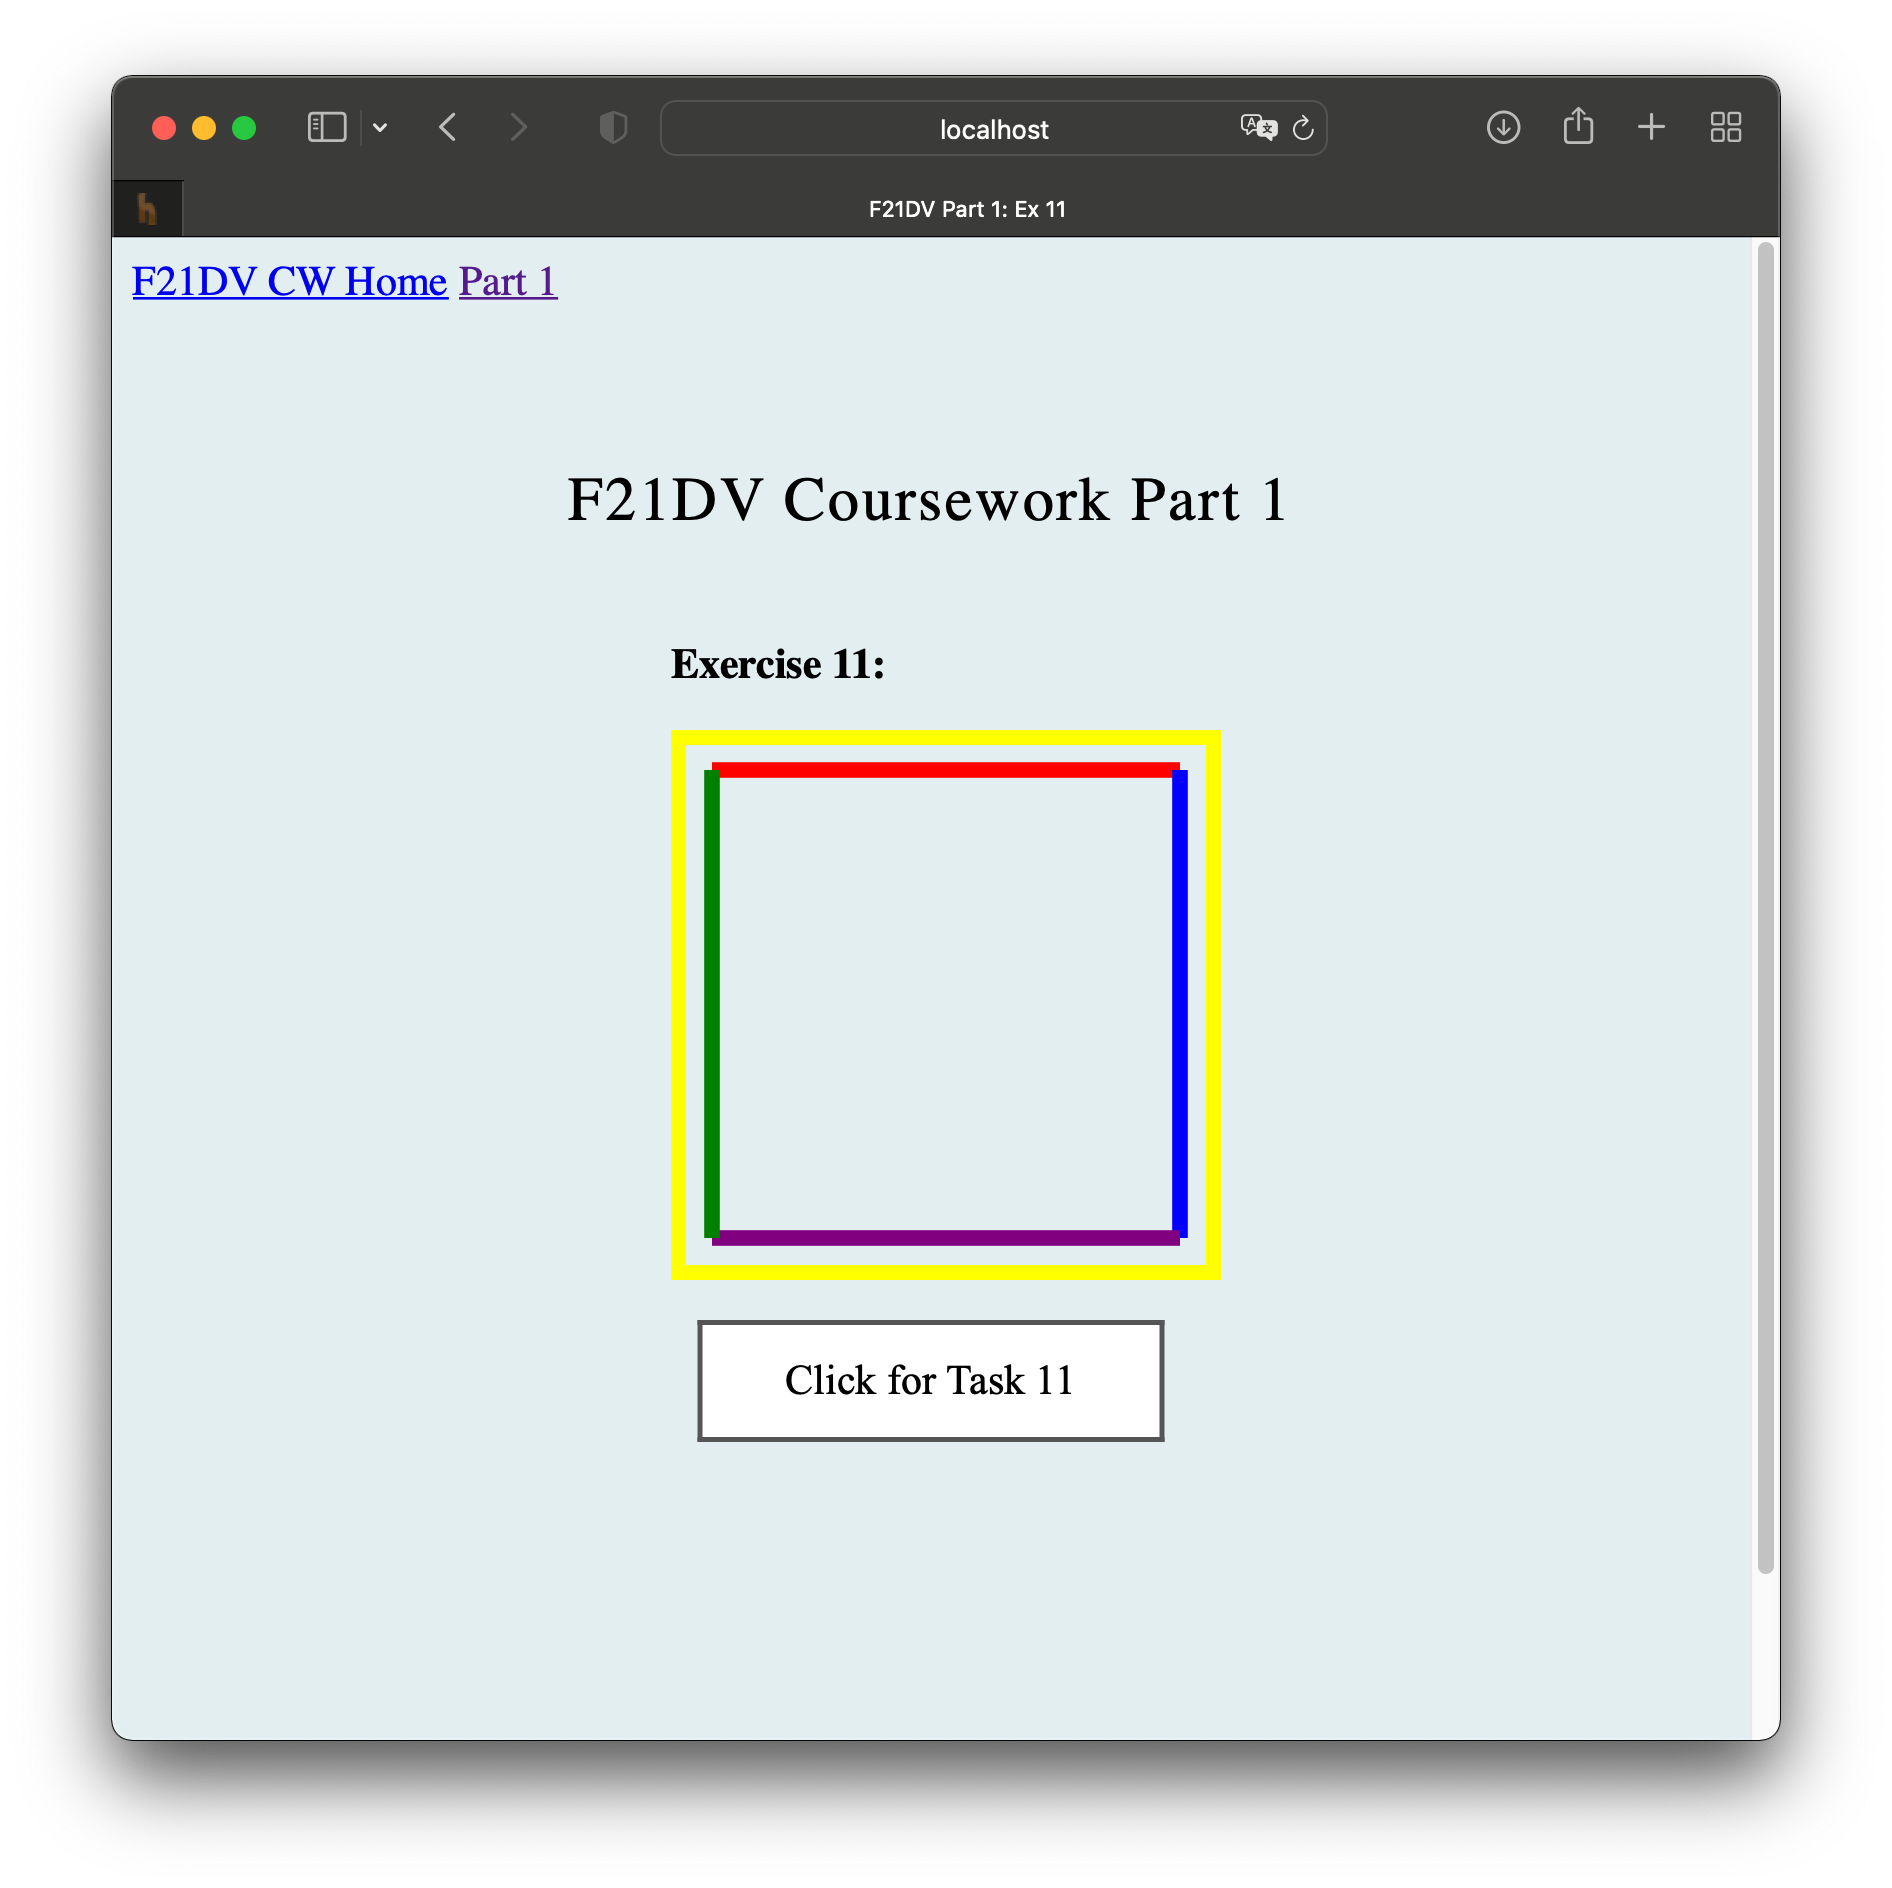
\includegraphics[width = 8cm]{images/ex11_2.png}
    \label{fig:ex11}
    \caption{Exercise 11}
\end{figure}
\FloatBarrier
% \lstinputlisting[language=JavaScript]{../../public/js/part1/task11.js}
Exercise 11, we first append a square yellow svg, and on the click of the button, 4 more lines are plot
in the middle of the svg.

\newpage
\section{Exercise 12 \& 13}
\begin{figure}[!ht]
    \centering
    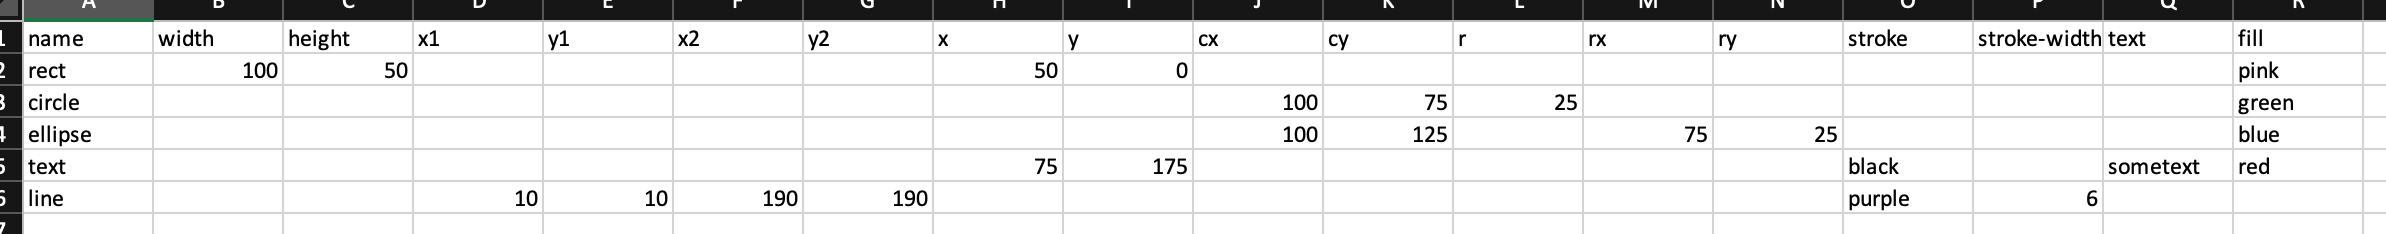
\includegraphics[width = \textwidth]{images/ex12_3.png}
    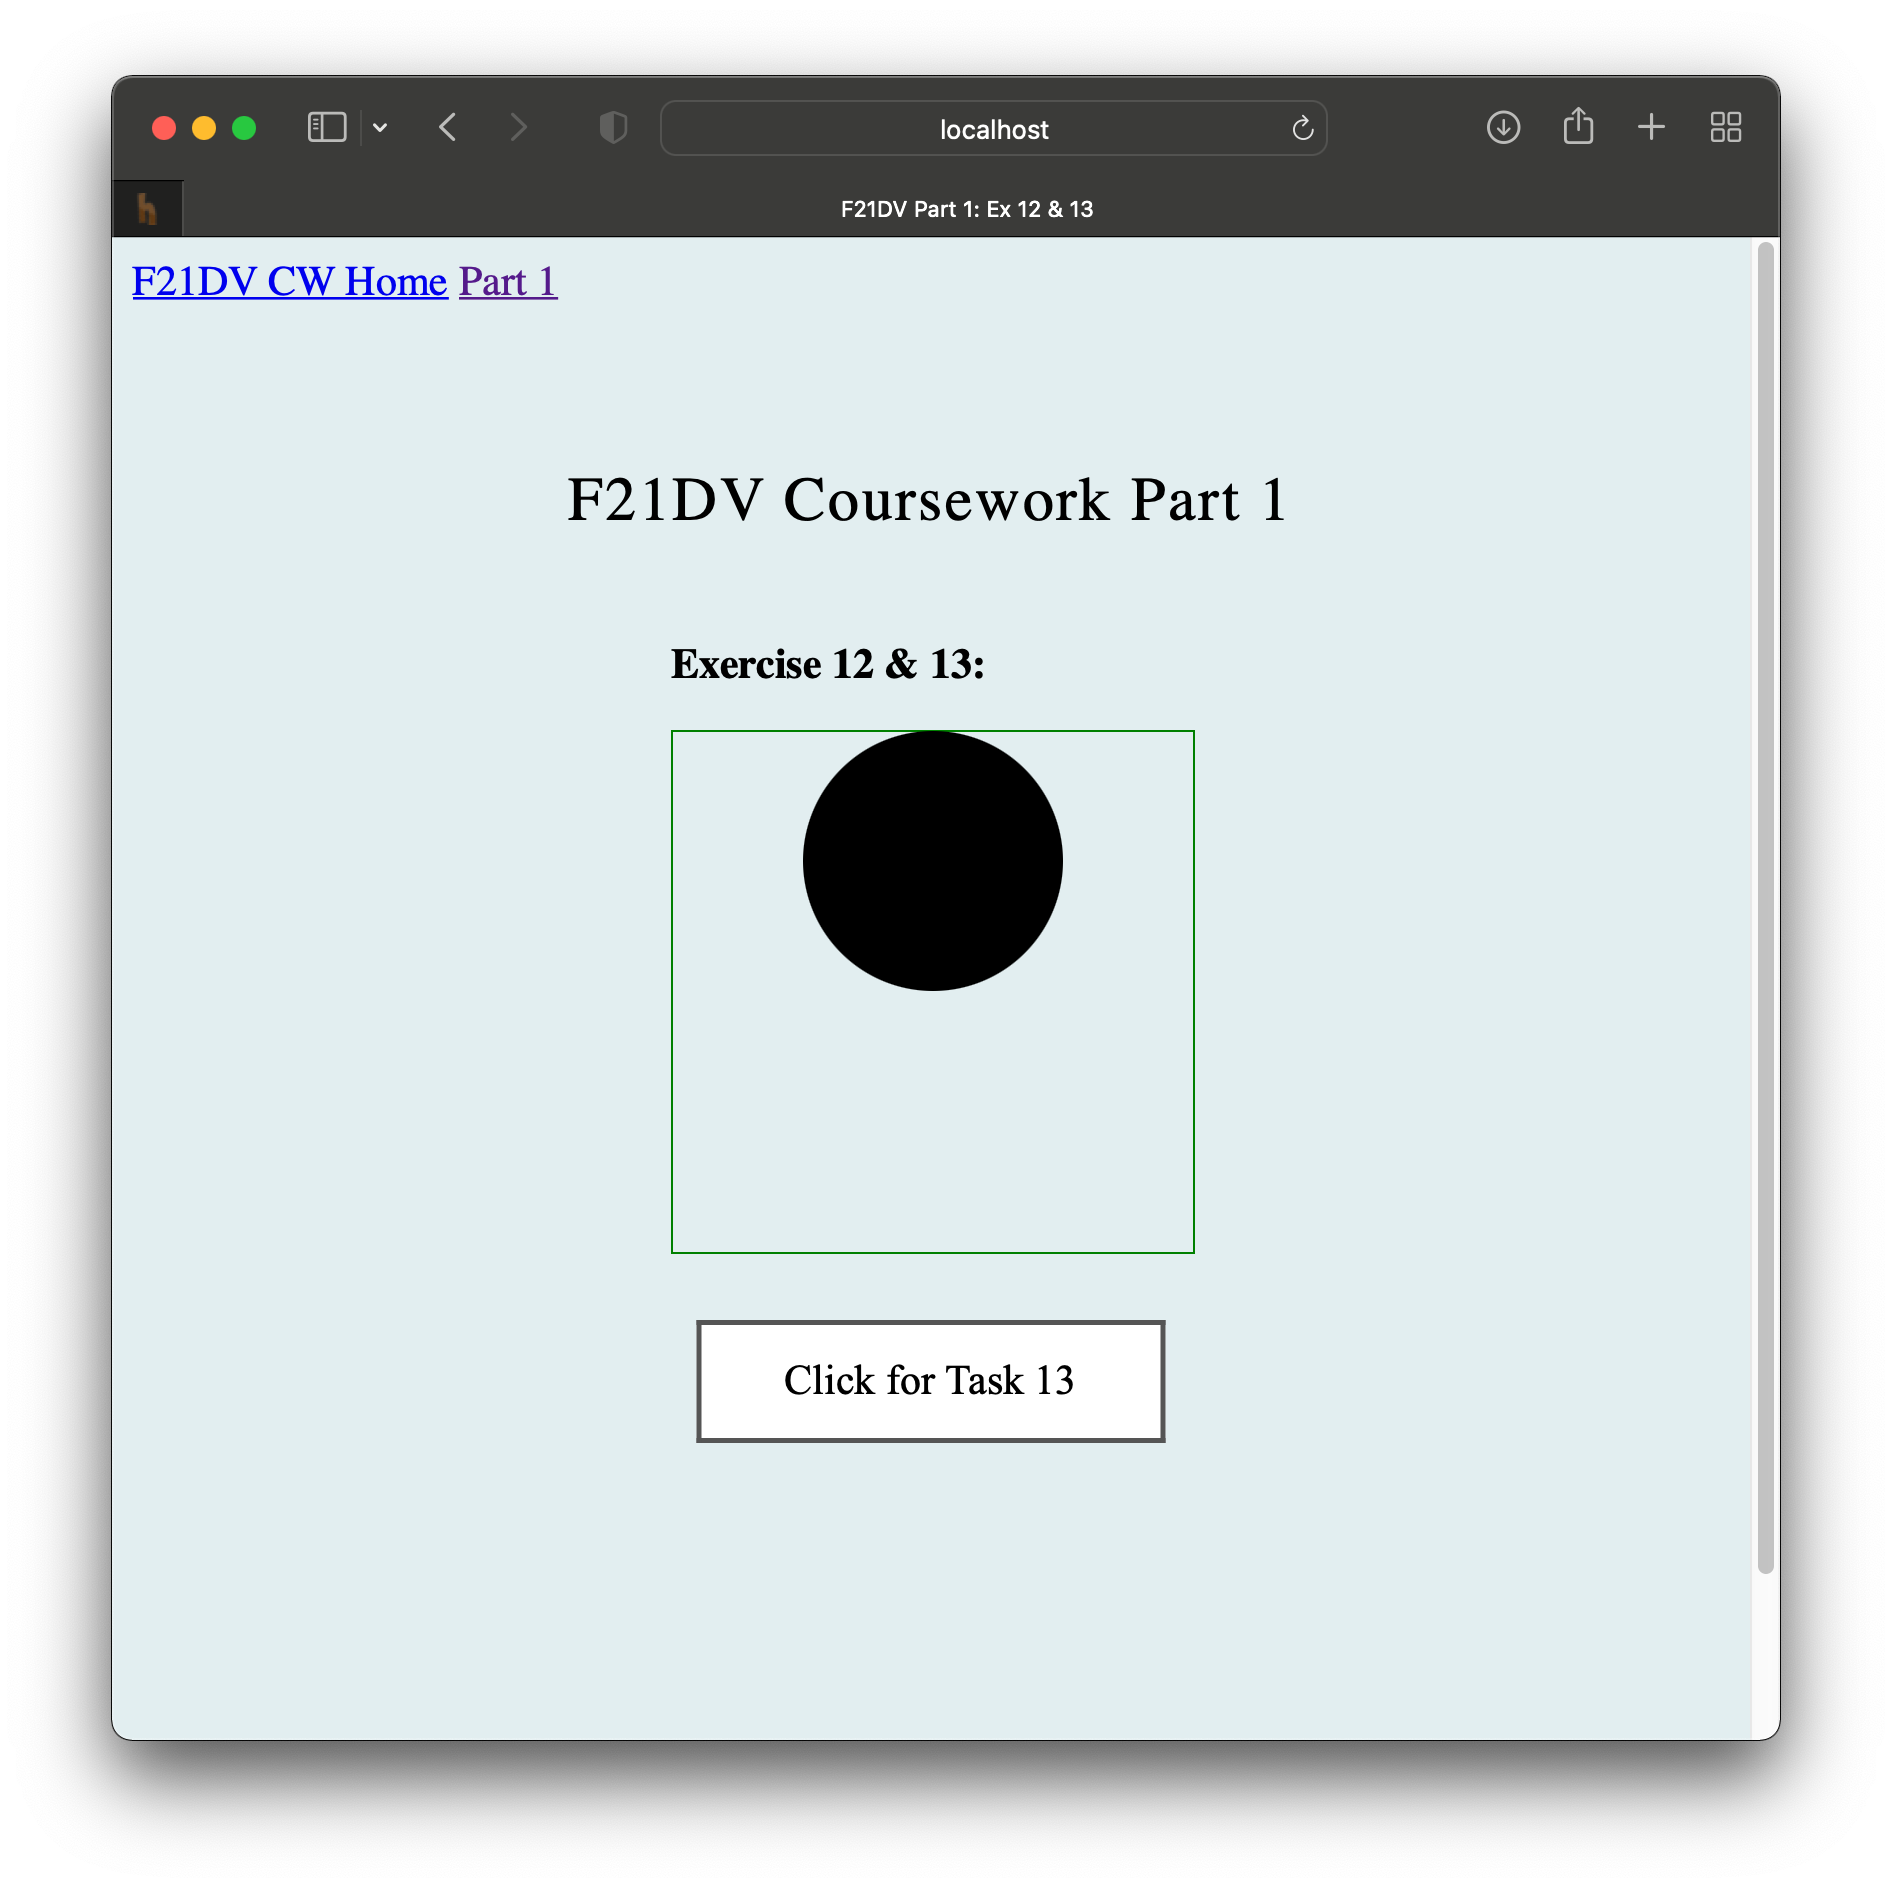
\includegraphics[width = 8cm]{images/ex12_1.png}
    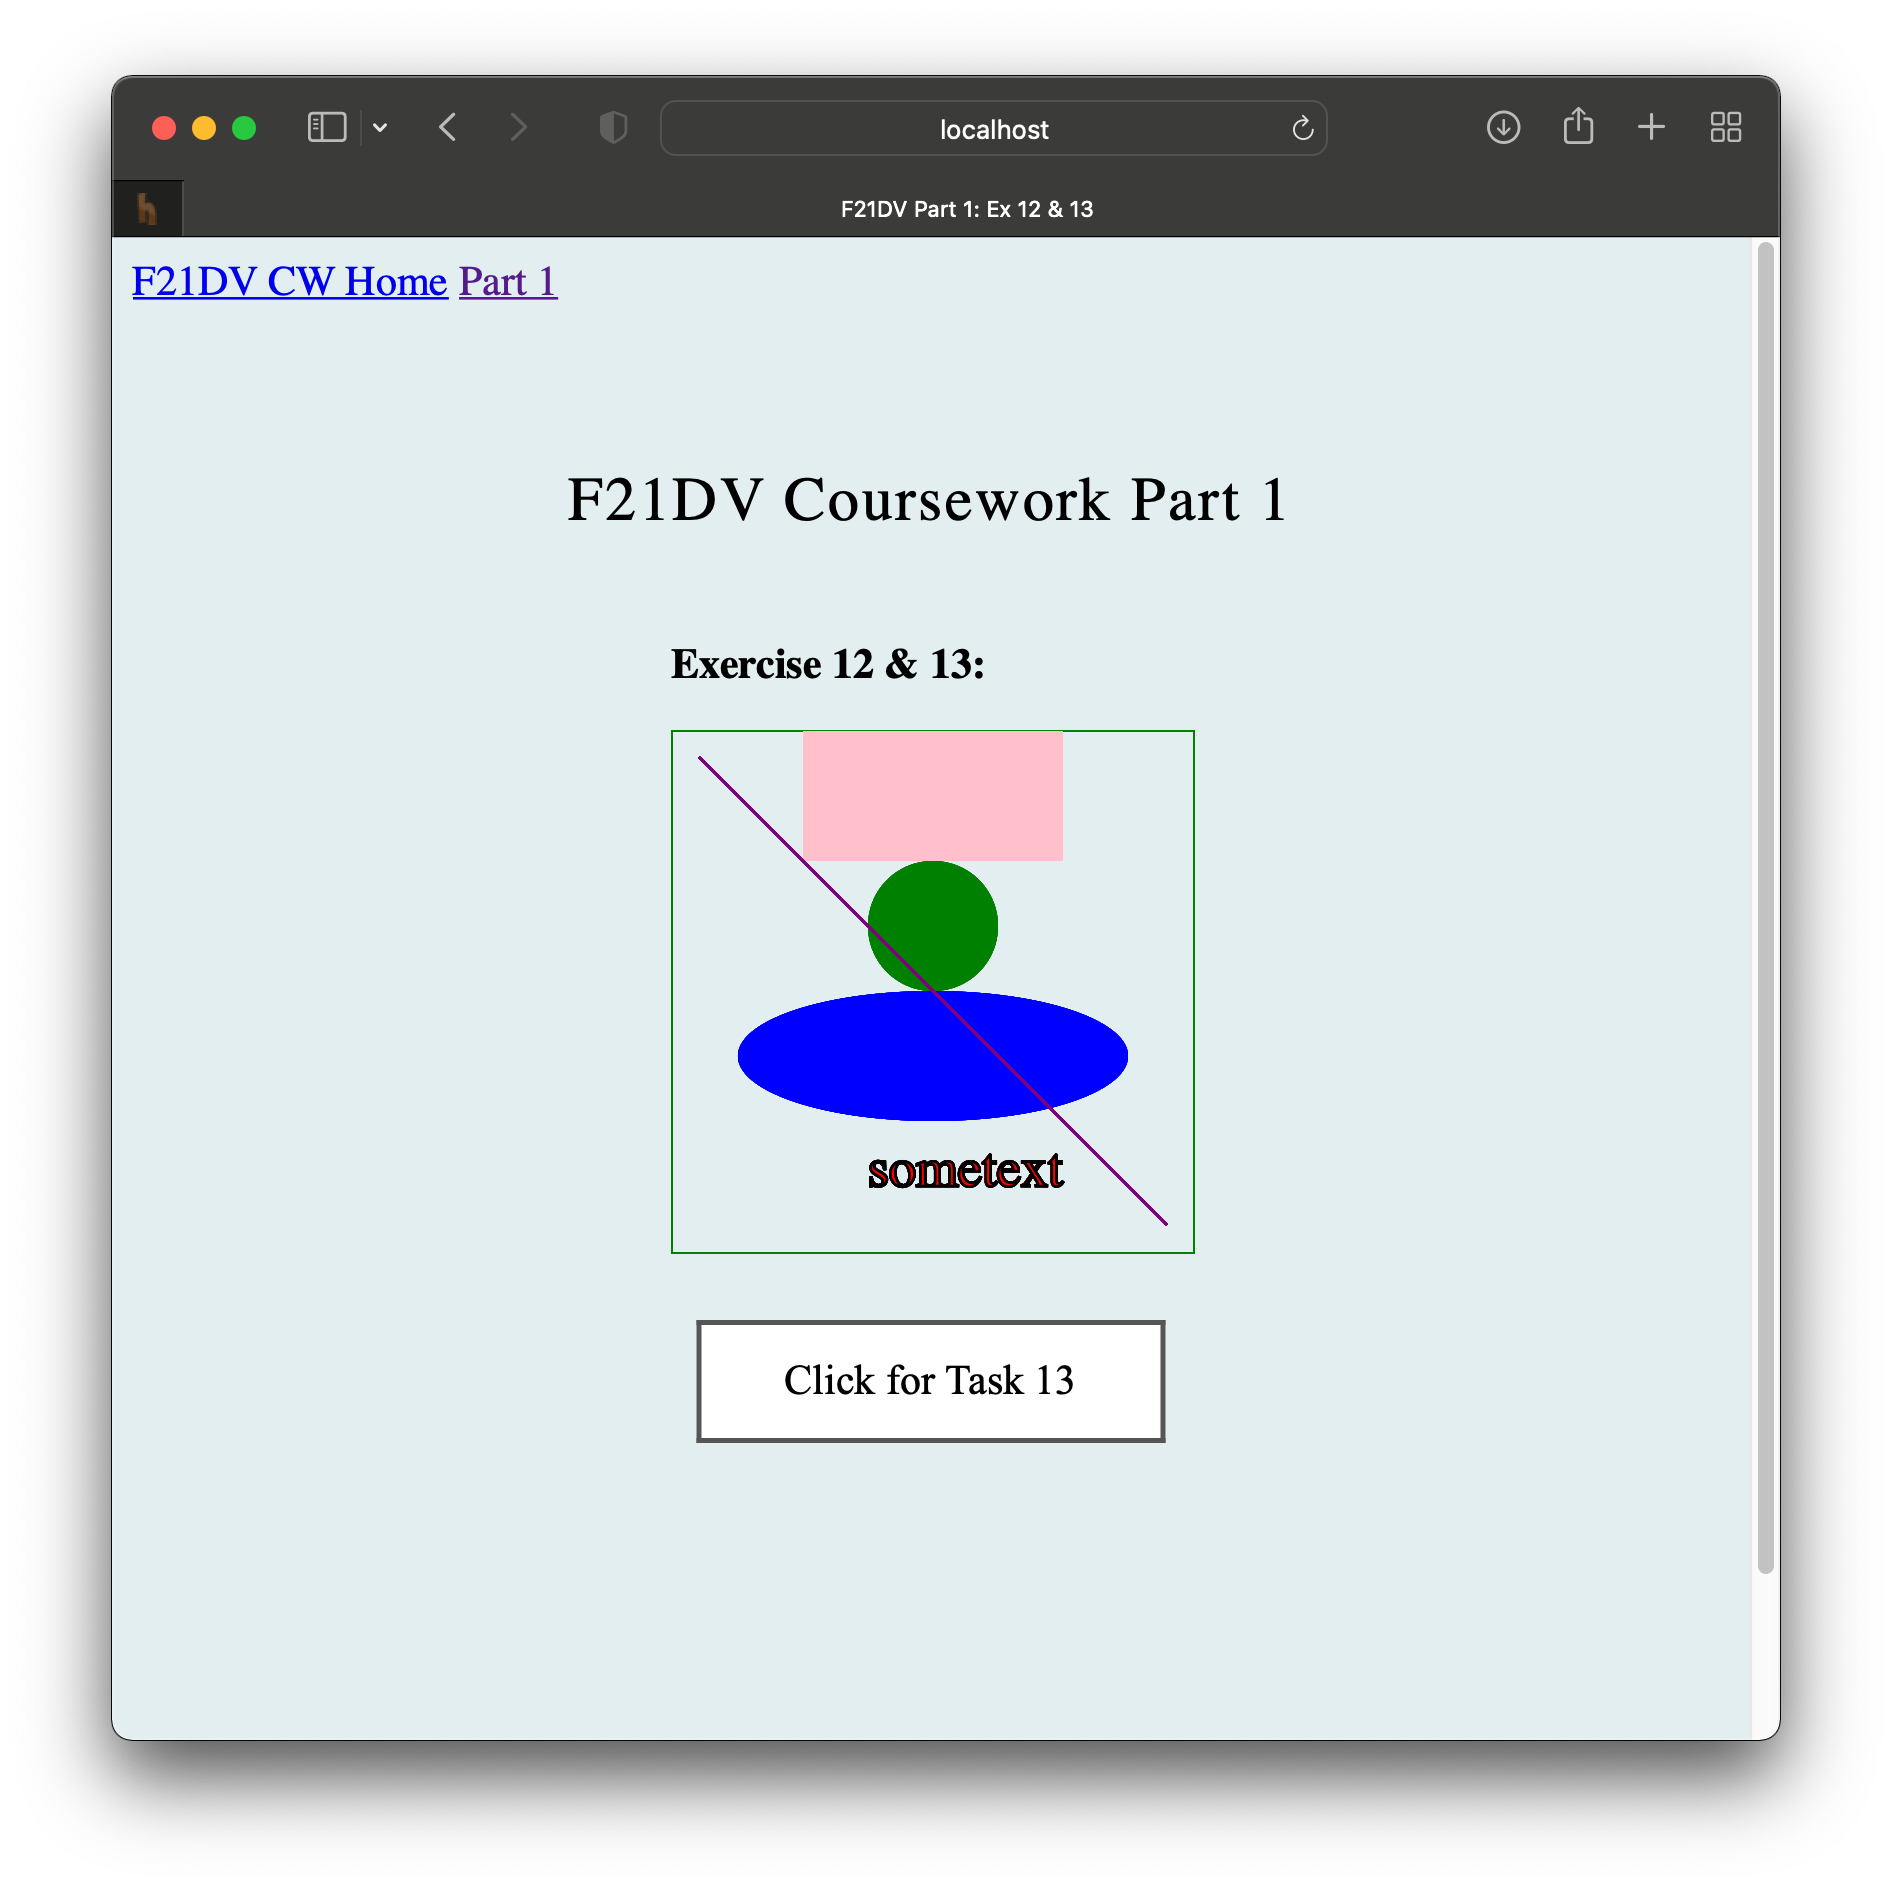
\includegraphics[width = 8cm]{images/ex12_2.png}
    \label{fig:ex12}
    \caption{Exercise 12 \& 13}
\end{figure}
\FloatBarrier
\lstinputlisting[language=JavaScript]{../../public/js/part1/task12n13.js}
This exercise starts off with reading the CSV data, as shown on top of figure \ref{fig:ex12}. For each
shape to be plot on, we enter its relevant attribute values and leave the irrelevant ones empty.\\
\par Next, upon the click of the button, there would first be a filtering of the data, where only
relevant (non-empty) attributes key-value pair is kept, in temporary local variable | \verb|data|. For 
shapes with lesser attributes, we append more dummy data, just so that the number of attributes are all
the same, allowing us to add shapes systematically, and to a point of not needing to have a few callback
functions. I have also added an exit transition for the initial `circle' shape, just to demonstrate the
use of a join function.

\newpage
\section{Exercise 14 \& 15}
\begin{figure}[!ht]
    \centering
    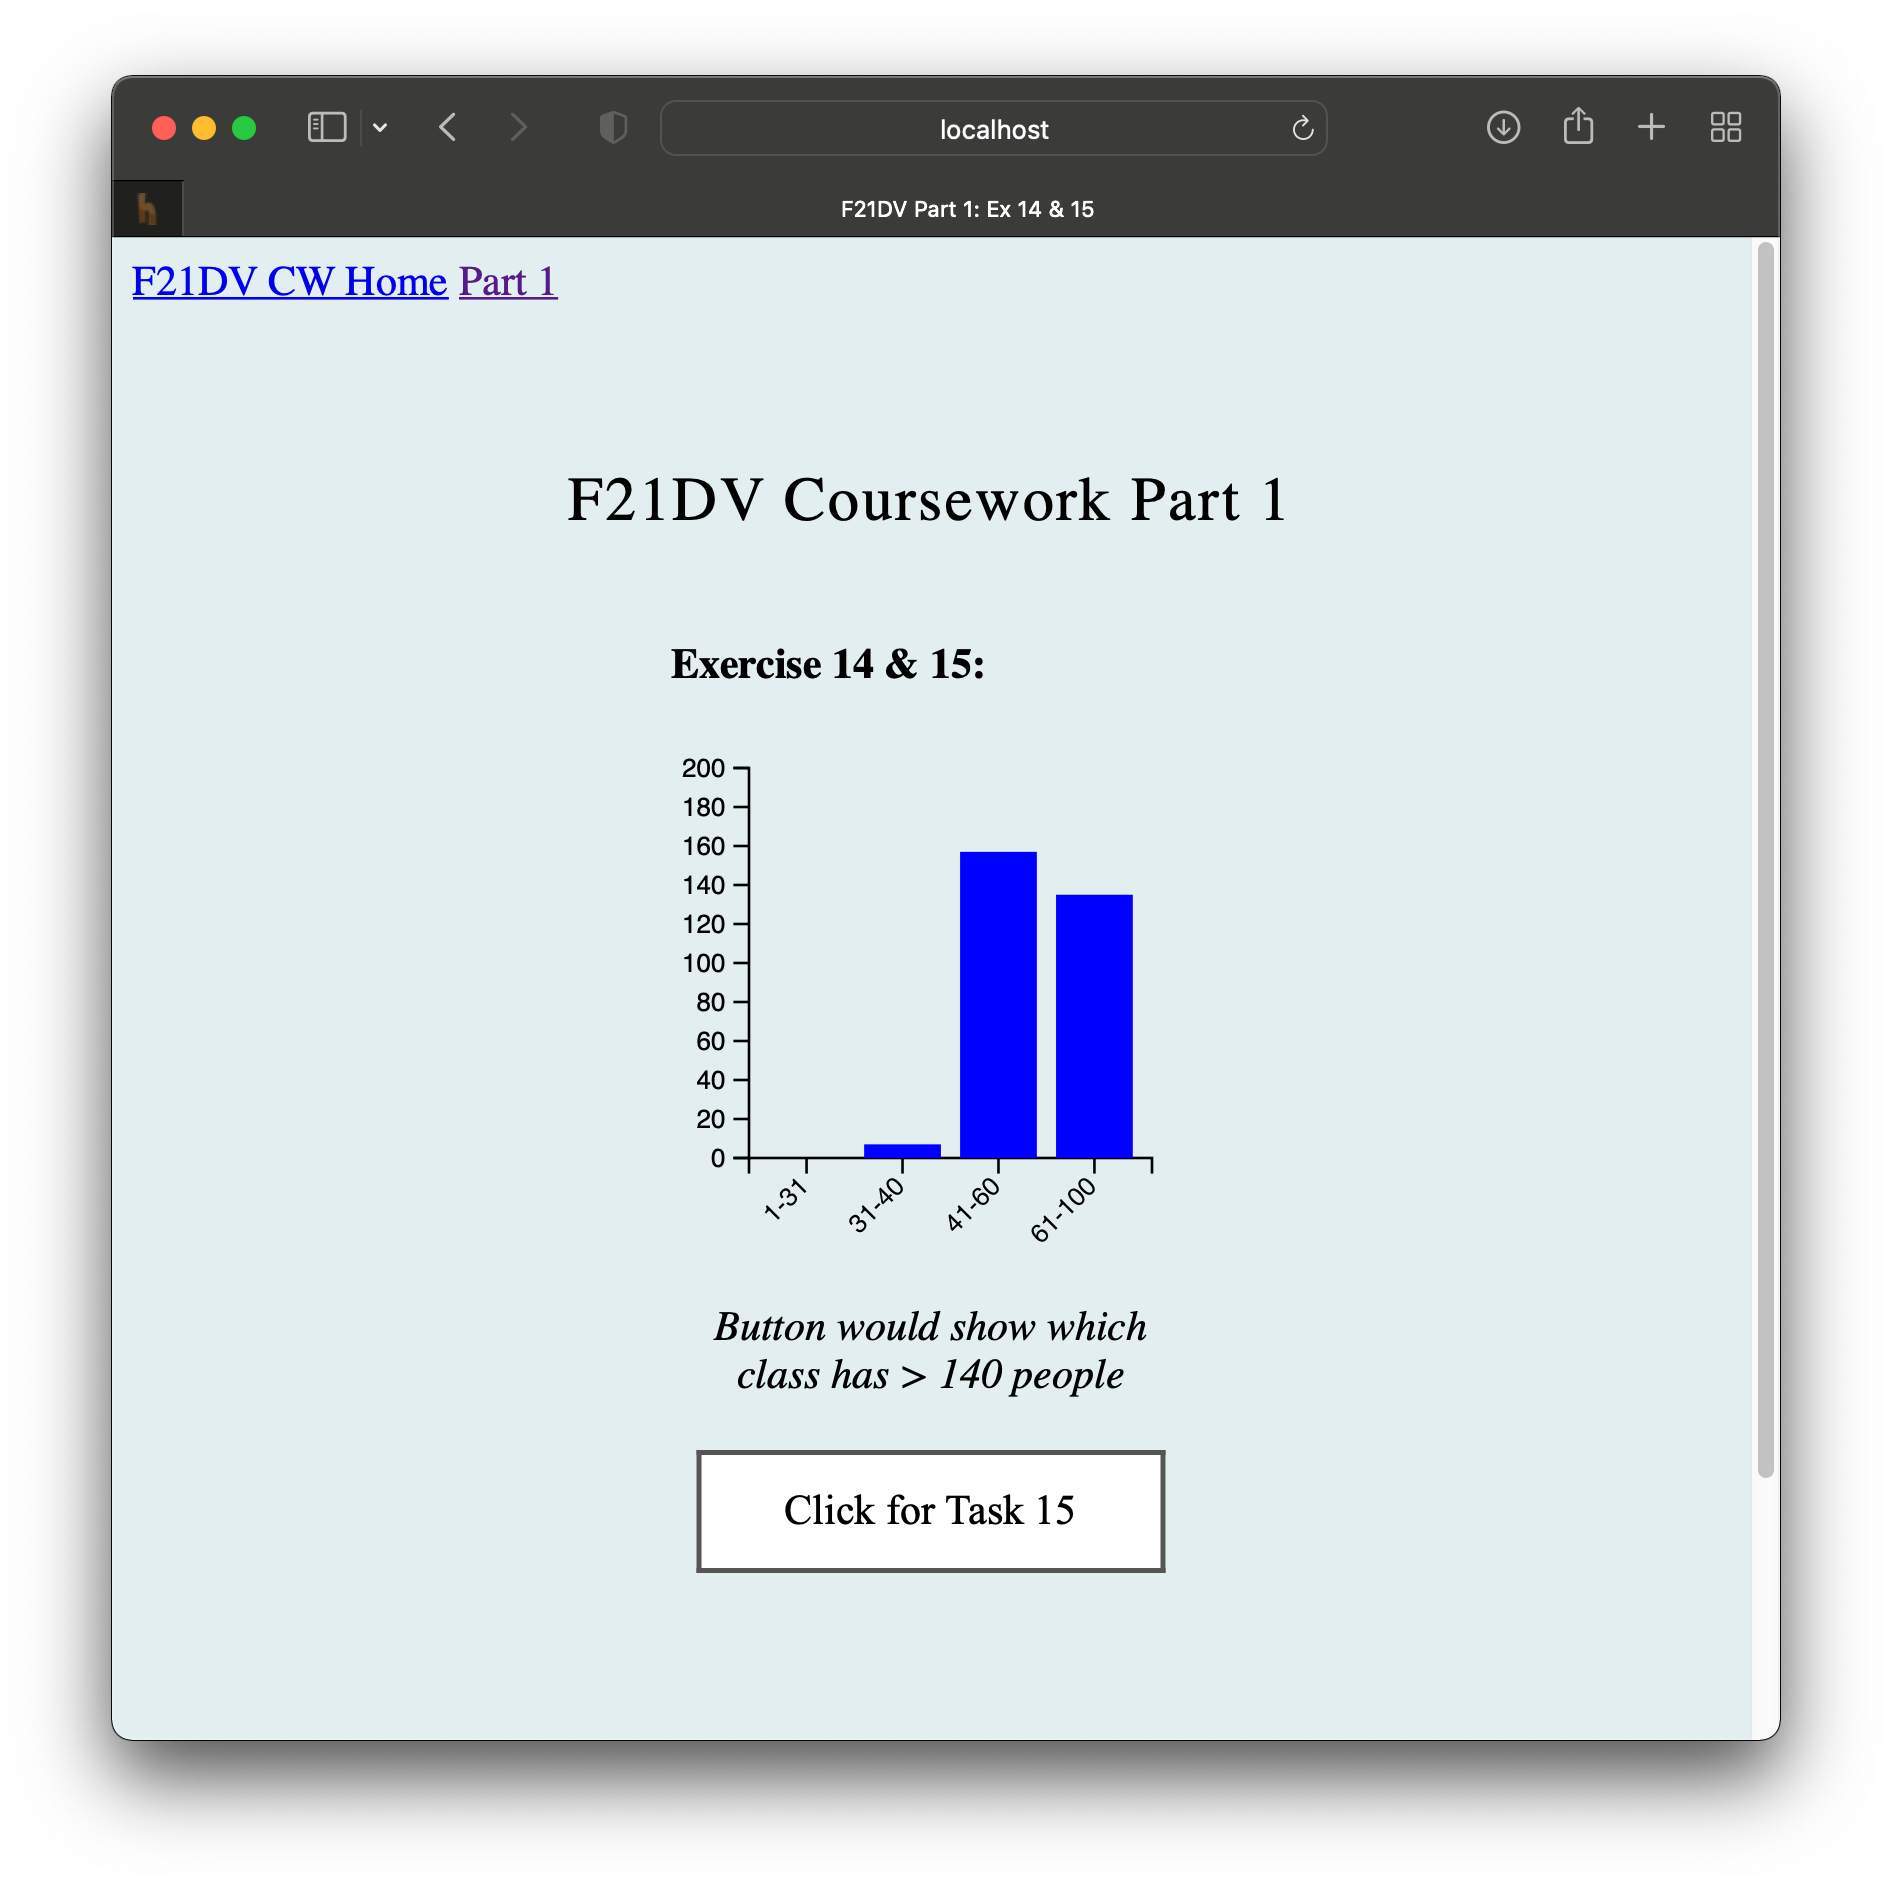
\includegraphics[width = 8cm]{images/ex14_1.png}
    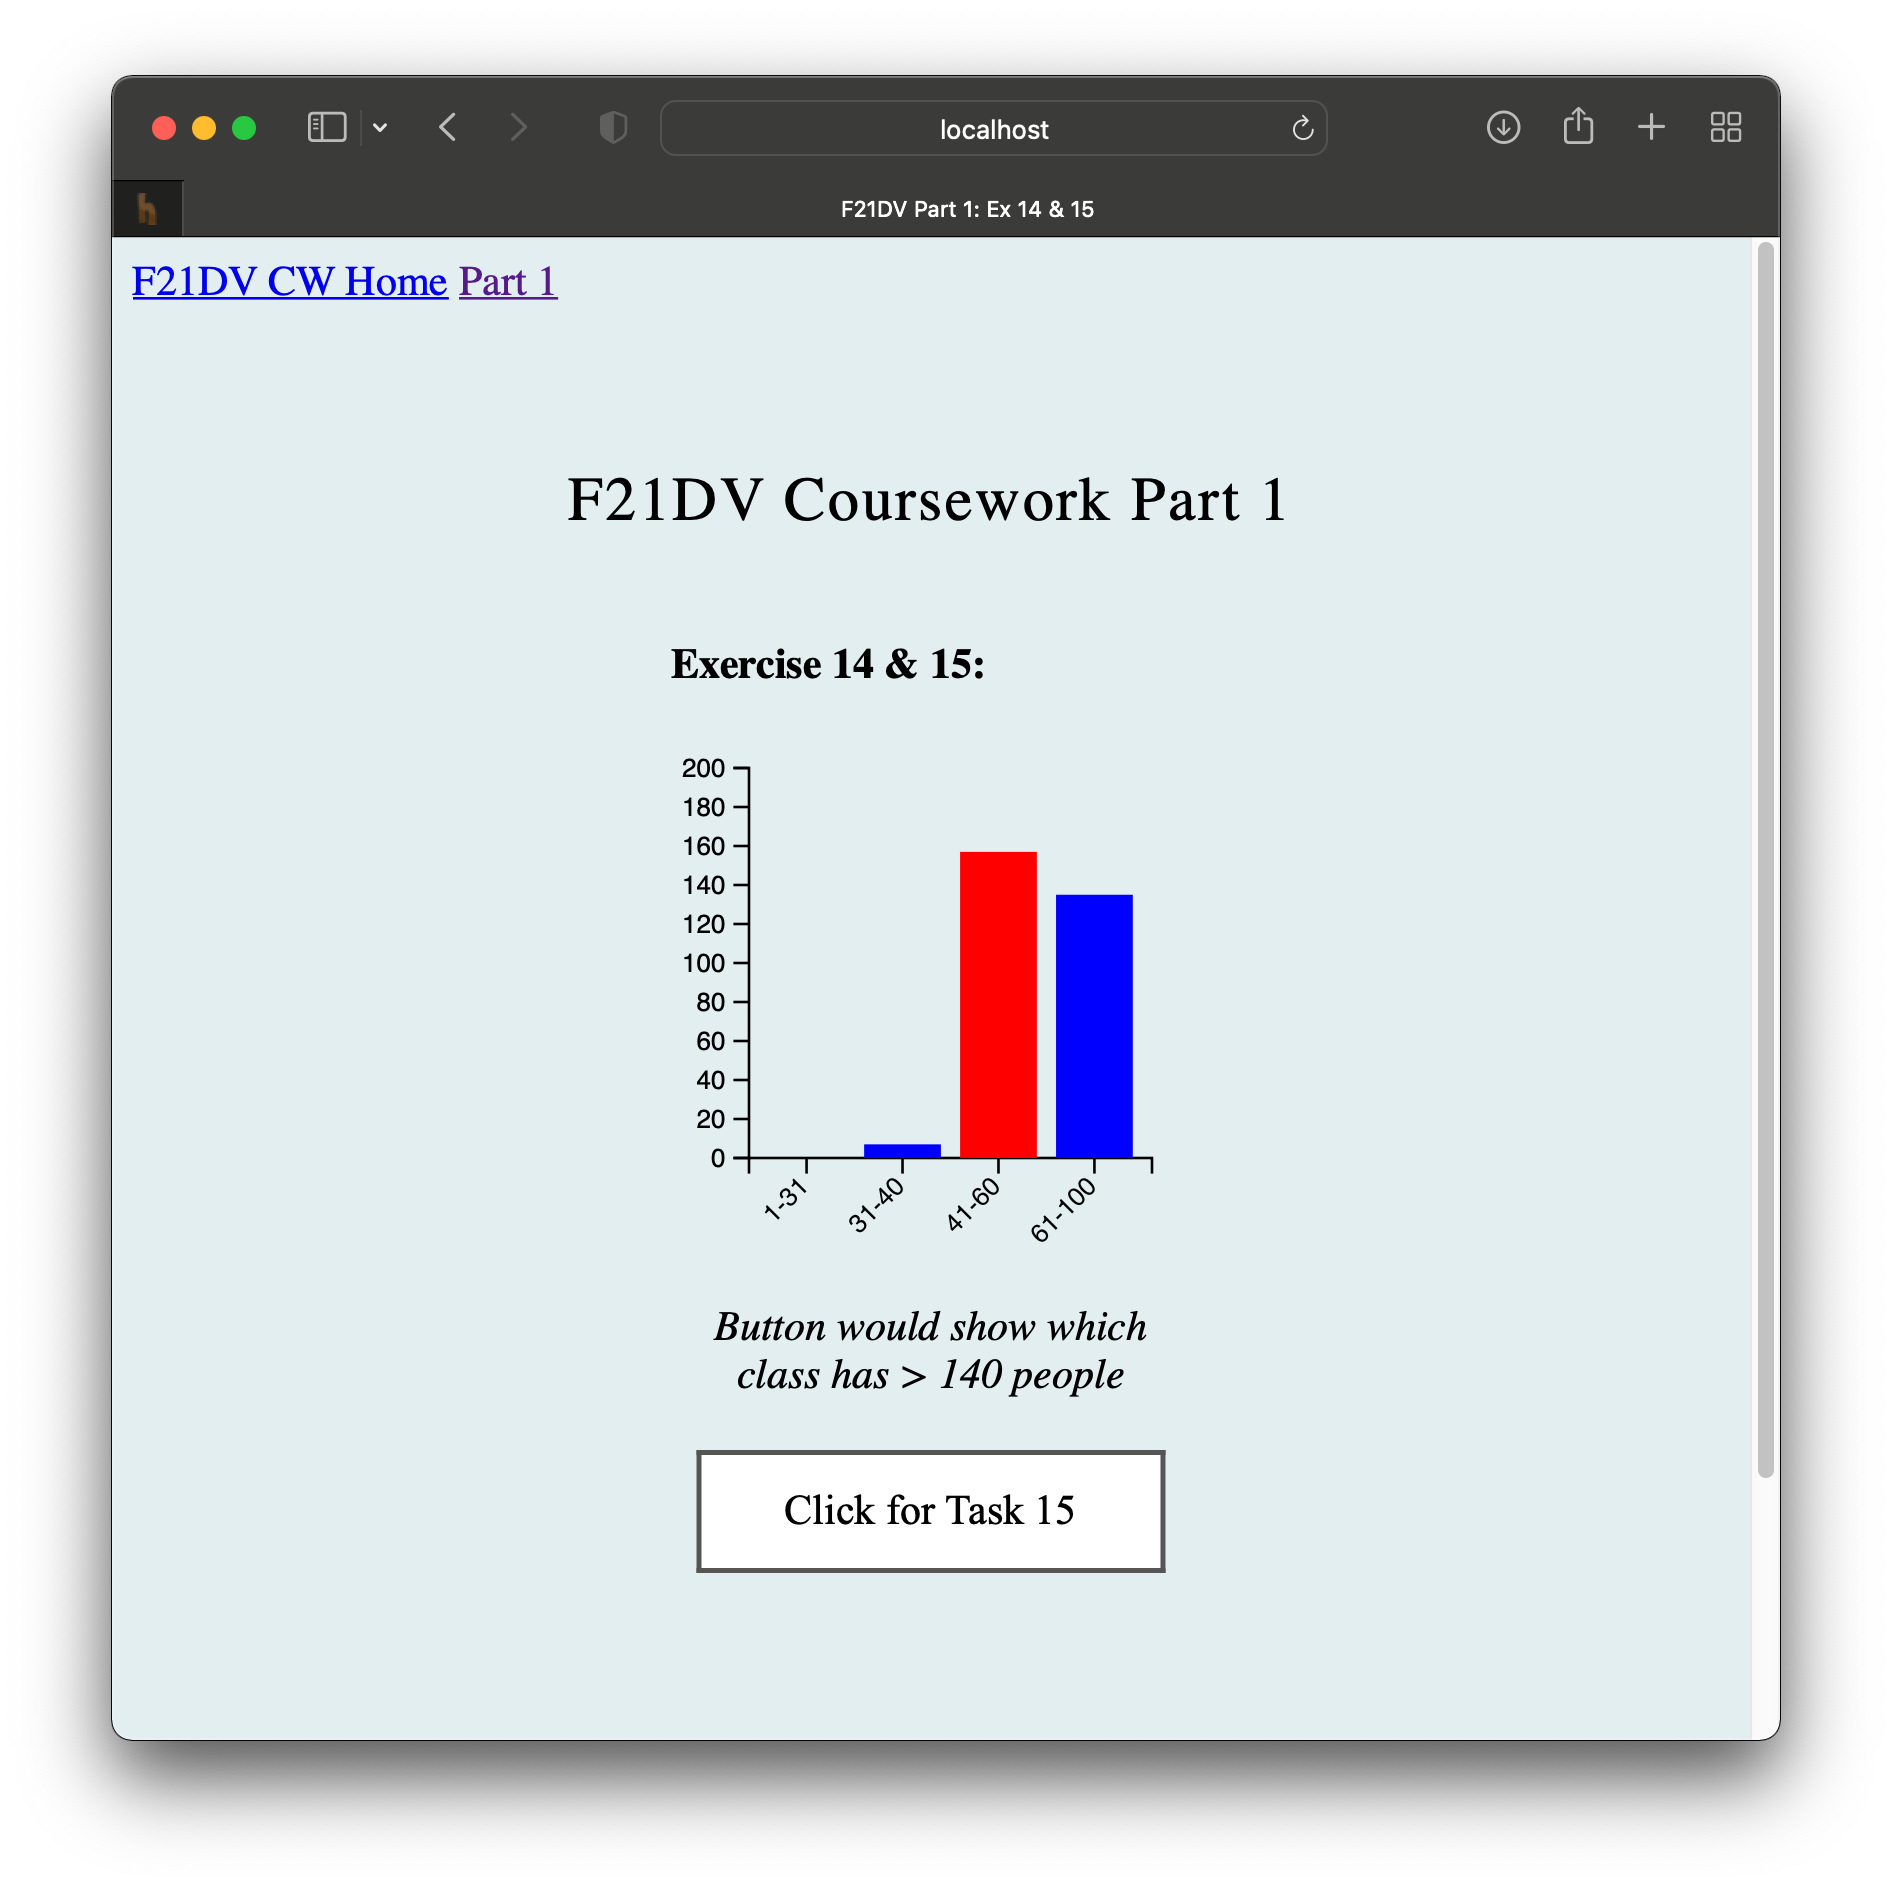
\includegraphics[width = 8cm]{images/ex14_2.png}
    \label{fig:ex14}
    \caption{Exercise 14 \& 15}
\end{figure}
\FloatBarrier
% \lstinputlisting[language=JavaScript]{../../public/js/part1/task14n15.js}
Exercise 14 \& 15 are the exercises using the exported async data from question 10. The question asked
only for rectangles, but I have added the axes on top of it. Hence, importing the data, we now can
categorise them according to value and scale them accordingly to determine the rectangle height in this
bar chart.\\
\par Upon click, the button would trigger an update action for the rectangle \verb|style| colours. If
the number of people with heart disease for said age group is more than 140, the colour of said rectangle
would be turned red.

\newpage
\section{Exercise 16}
\begin{figure}[!ht]
    \centering
    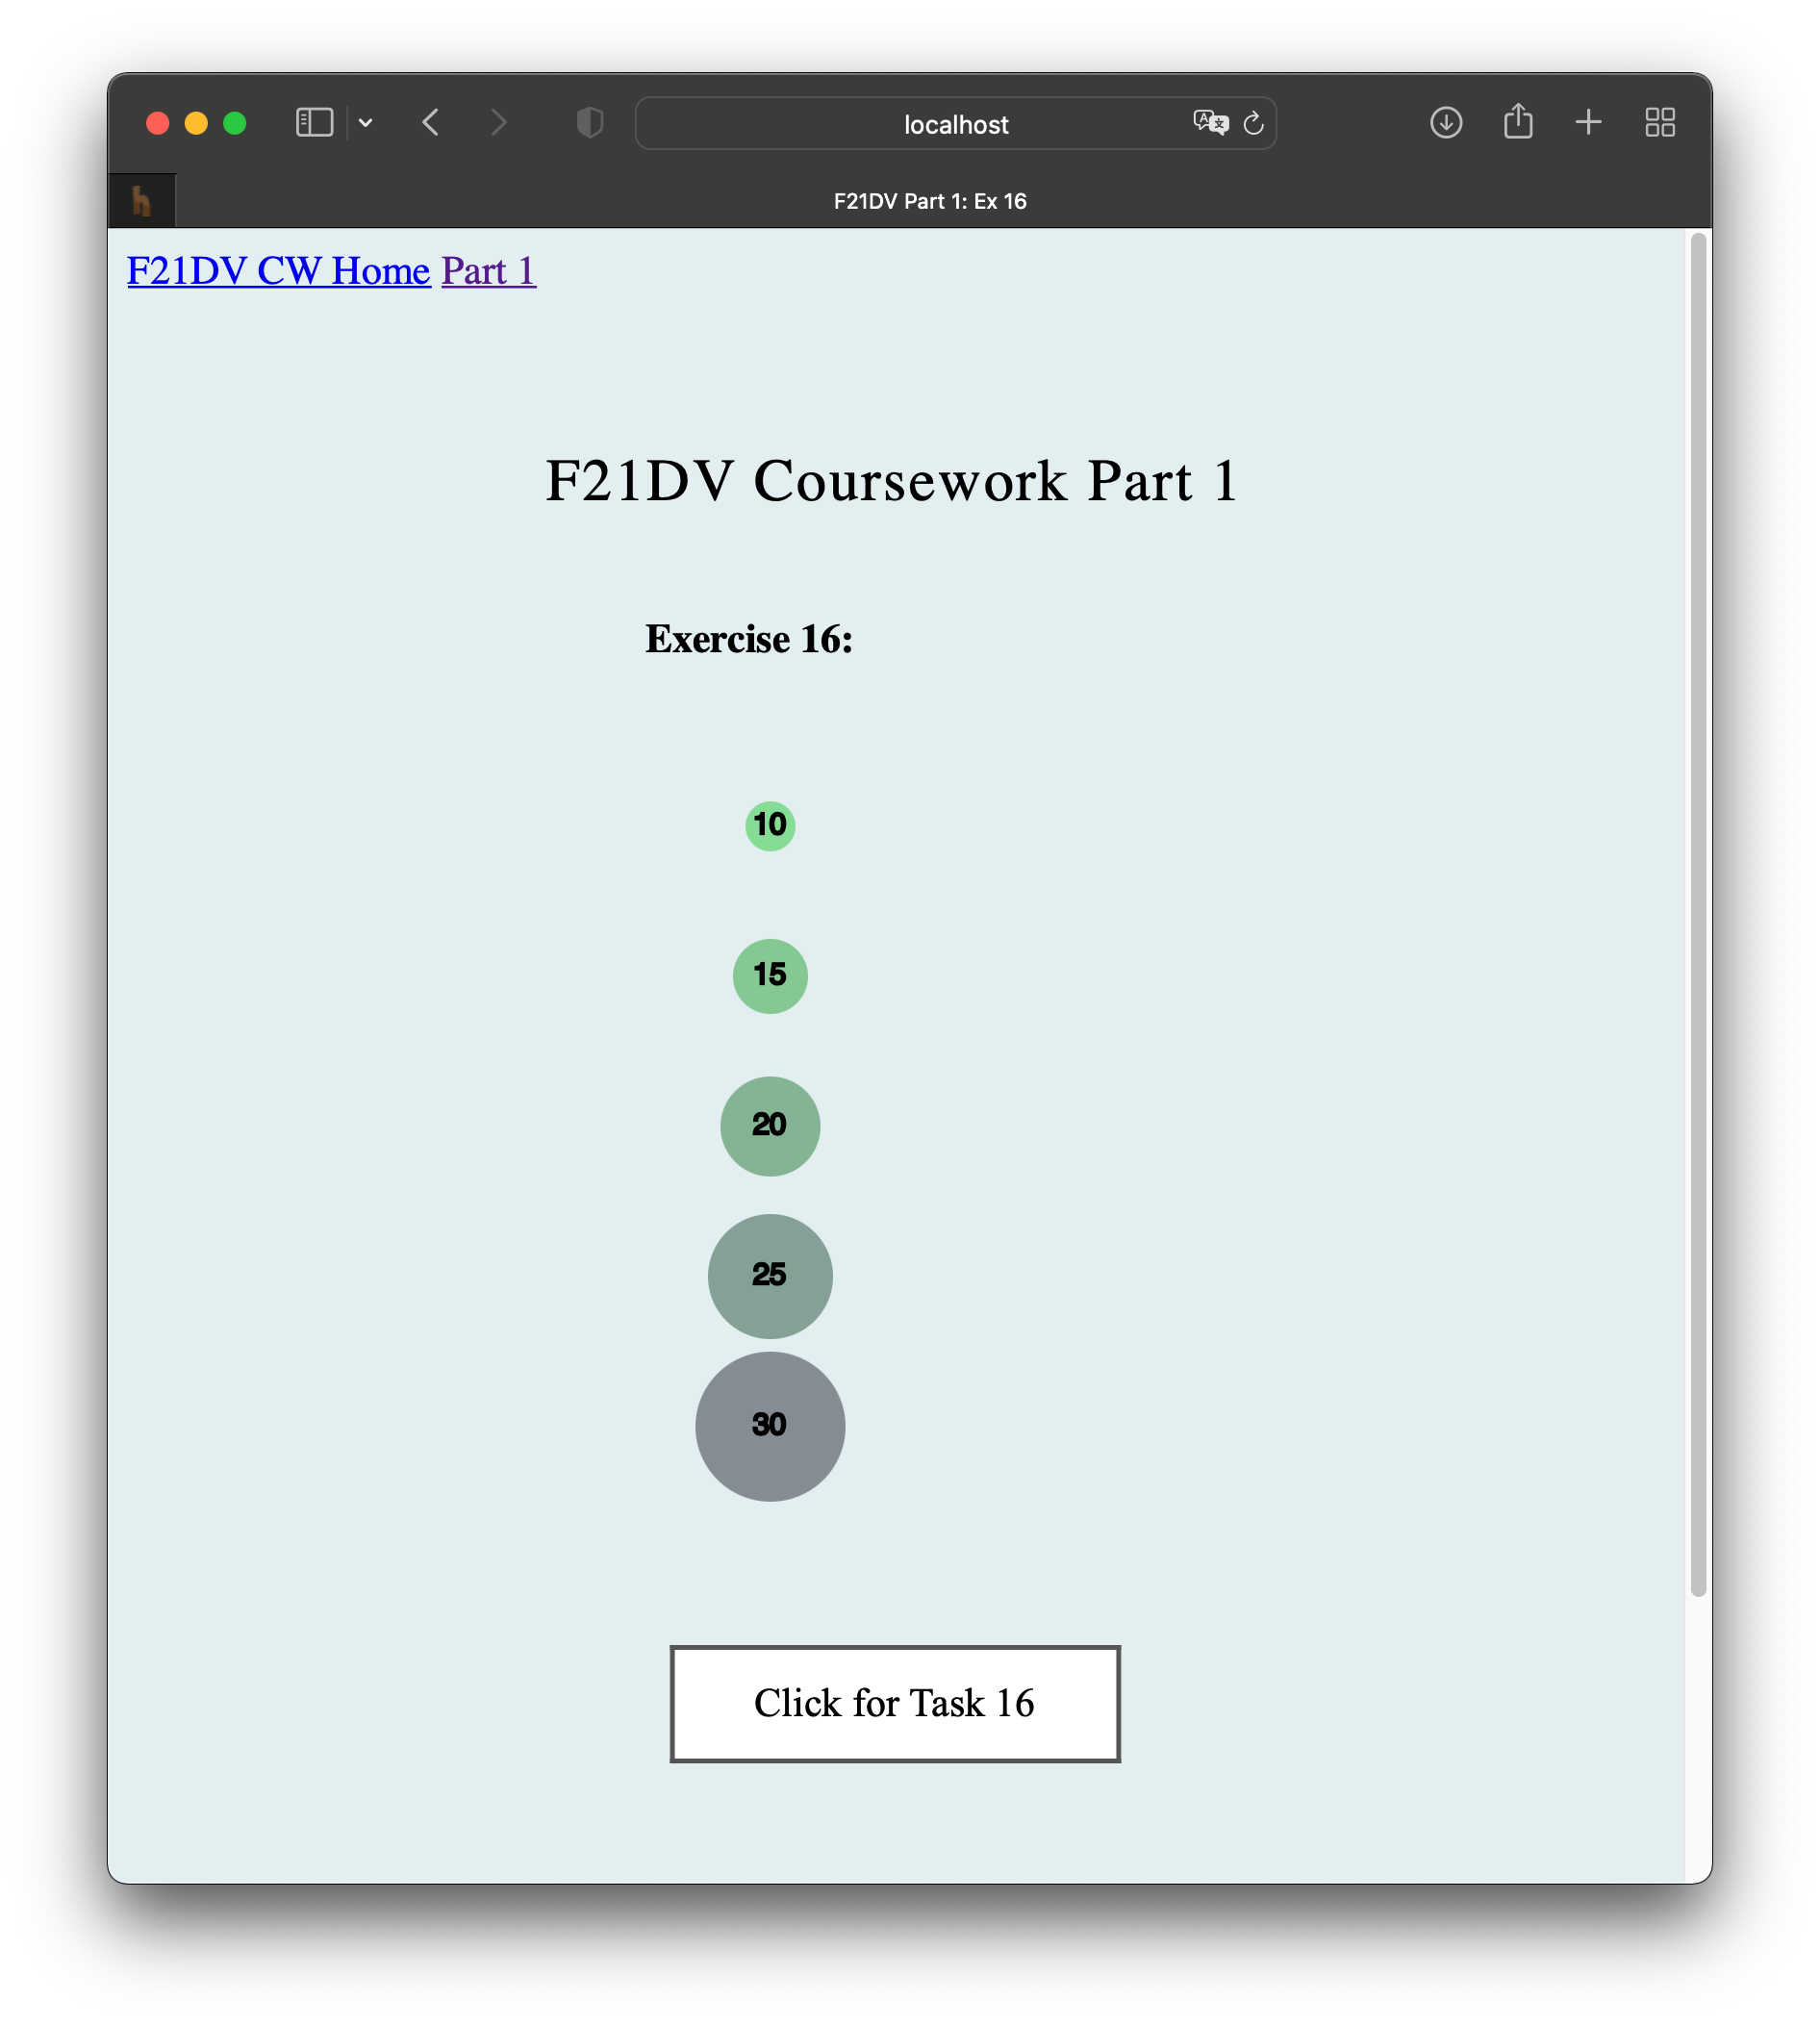
\includegraphics[width = 8cm]{images/ex16_1.png}
    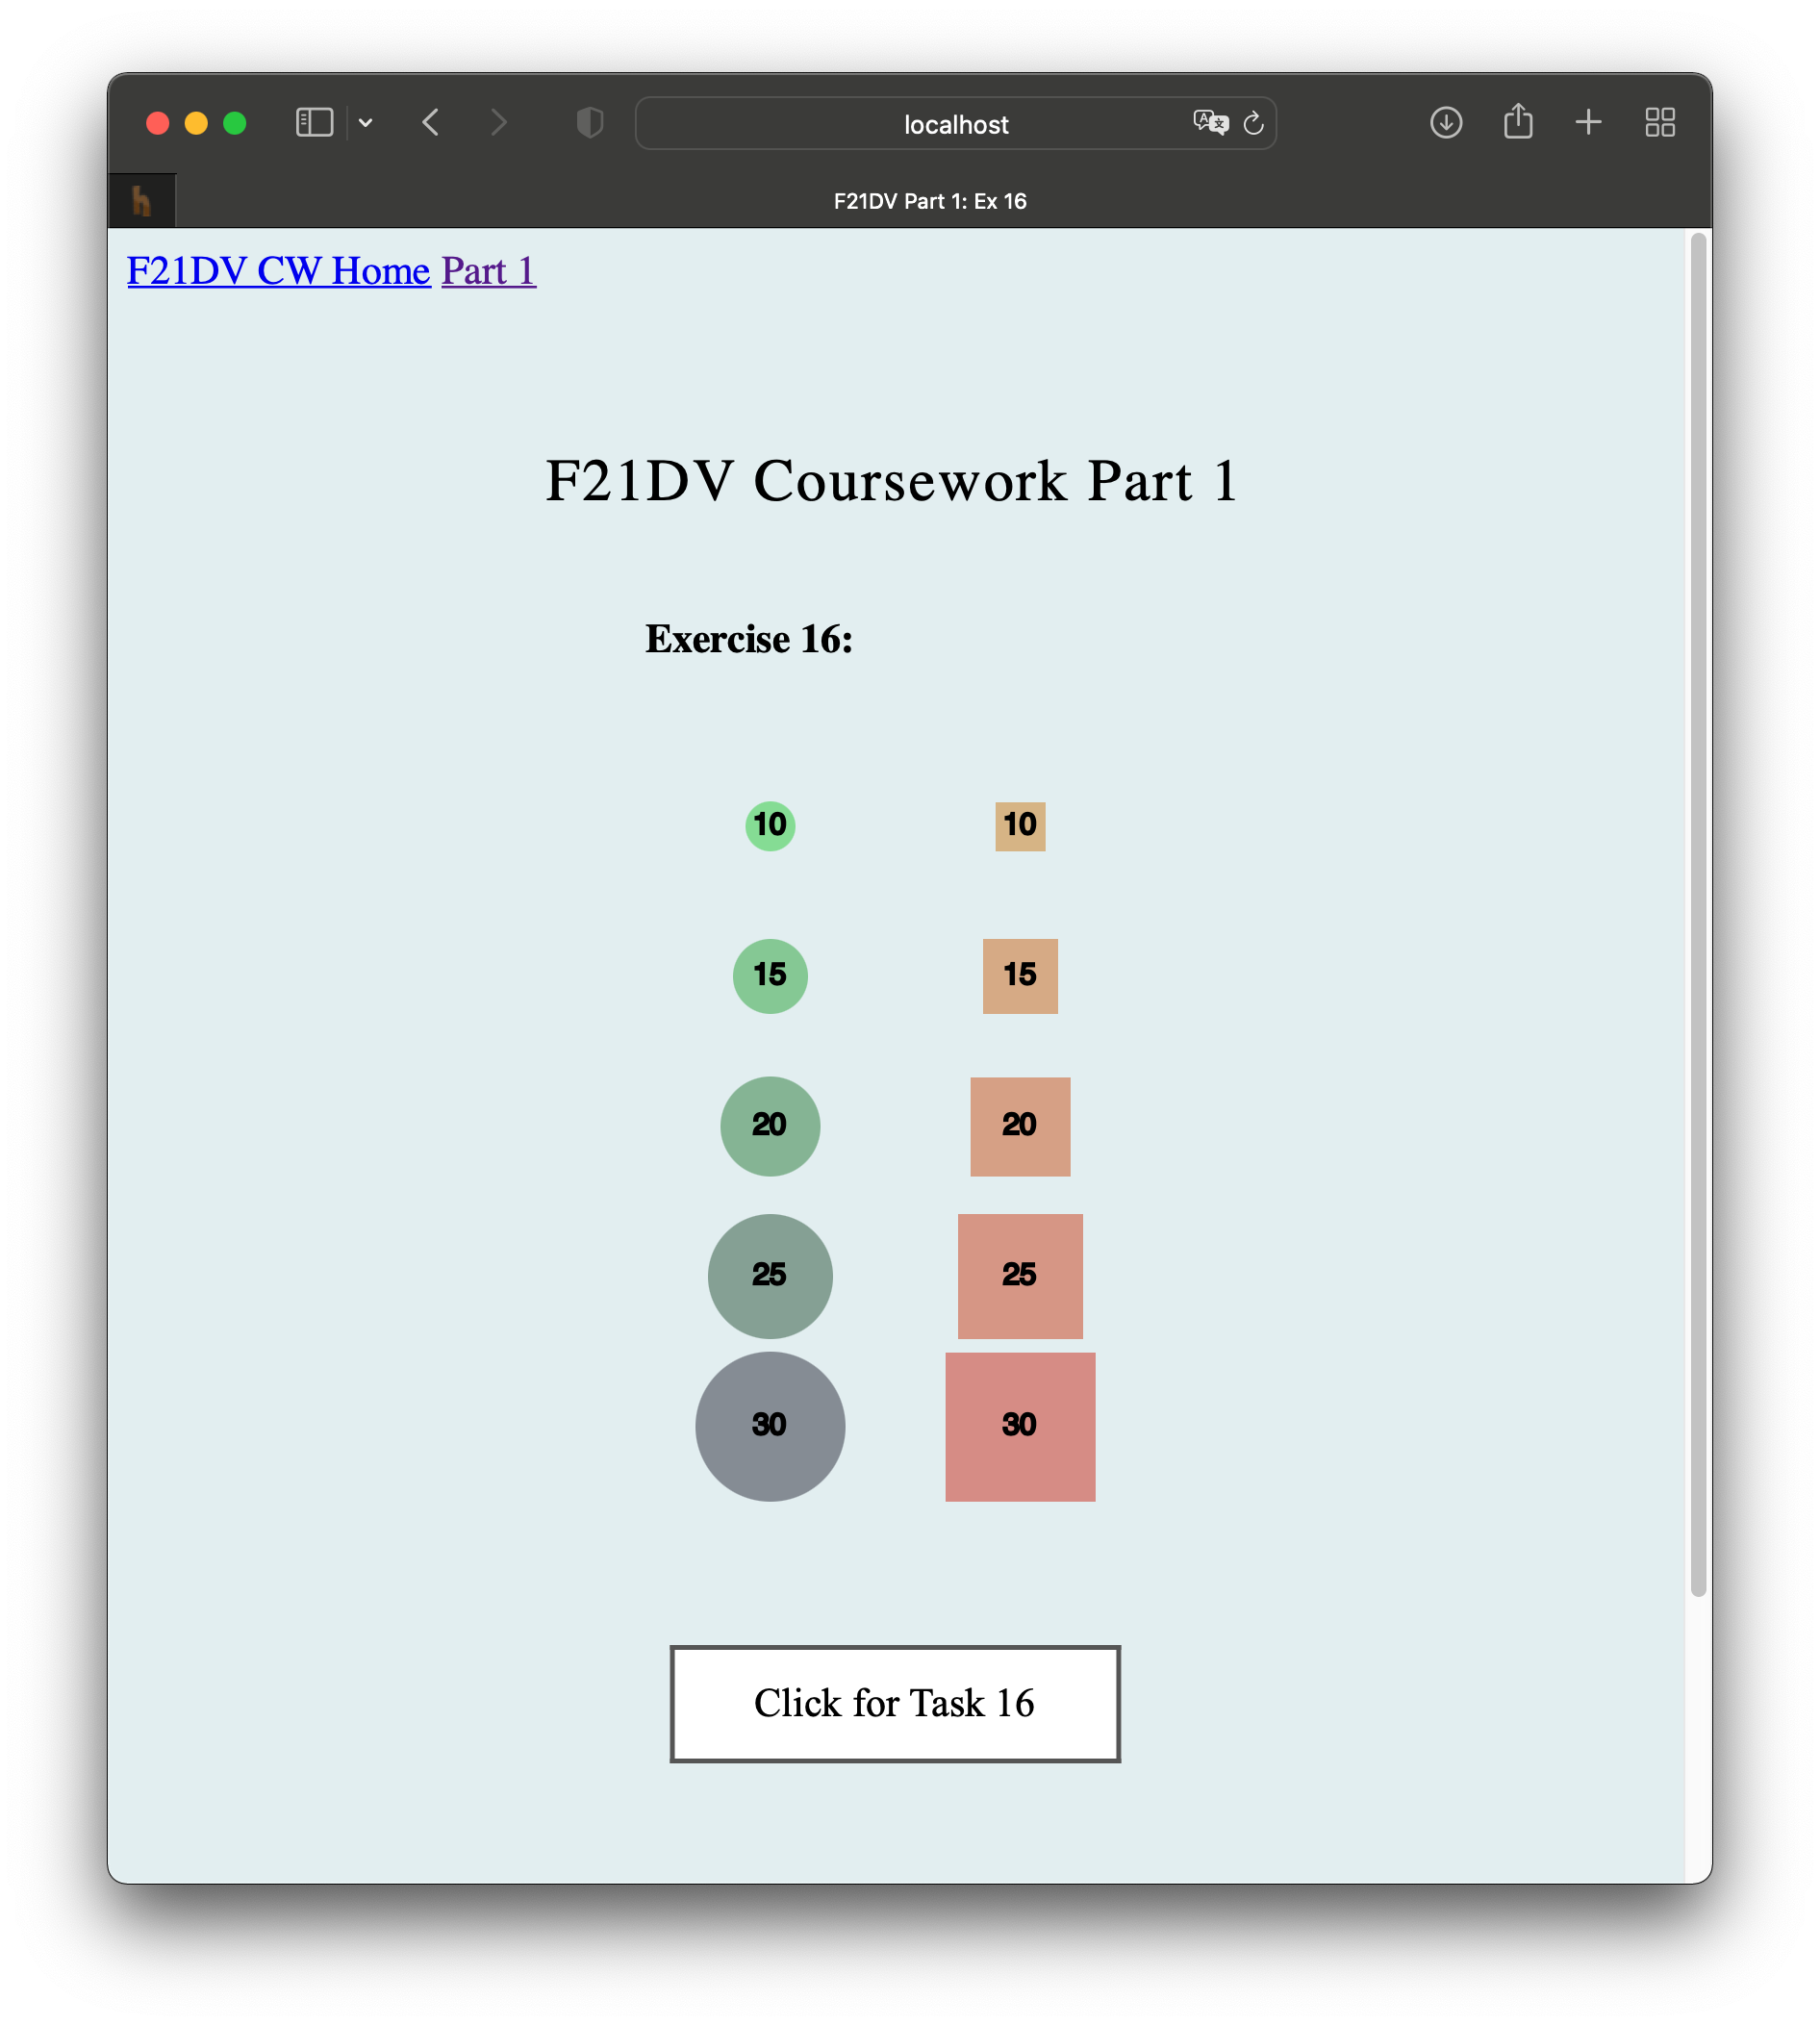
\includegraphics[width = 8cm]{images/ex16_2.png}
    \label{fig:ex16}
    \caption{Exercise 16}
\end{figure}
\FloatBarrier
% \lstinputlisting[language=JavaScript]{../../public/js/part1/task16.js}
Exercise 16 is about adding shapes based on the given data and its index within the data array. The 
example given shows how to add circles following the data values, which determines its size. The 
exercise also uses index numbers to determine its vertical axis translation. \\
\par By pressing the button, we would trigger the squares to appear. I have done the same
for the square, just instead of using the data values to set the length of the sides of square, I
multiply it by 2, just so that the height of the square would be the same as the diameter of the 
circle. The verticle translation is also based off the index of data points, but the difference is
that there is an extra few values in the horizontal translation of the squares, so that it can now 
be side by side to the circles. 

\newpage
\section{Exercise 17}
\begin{figure}[!ht]
    \centering
    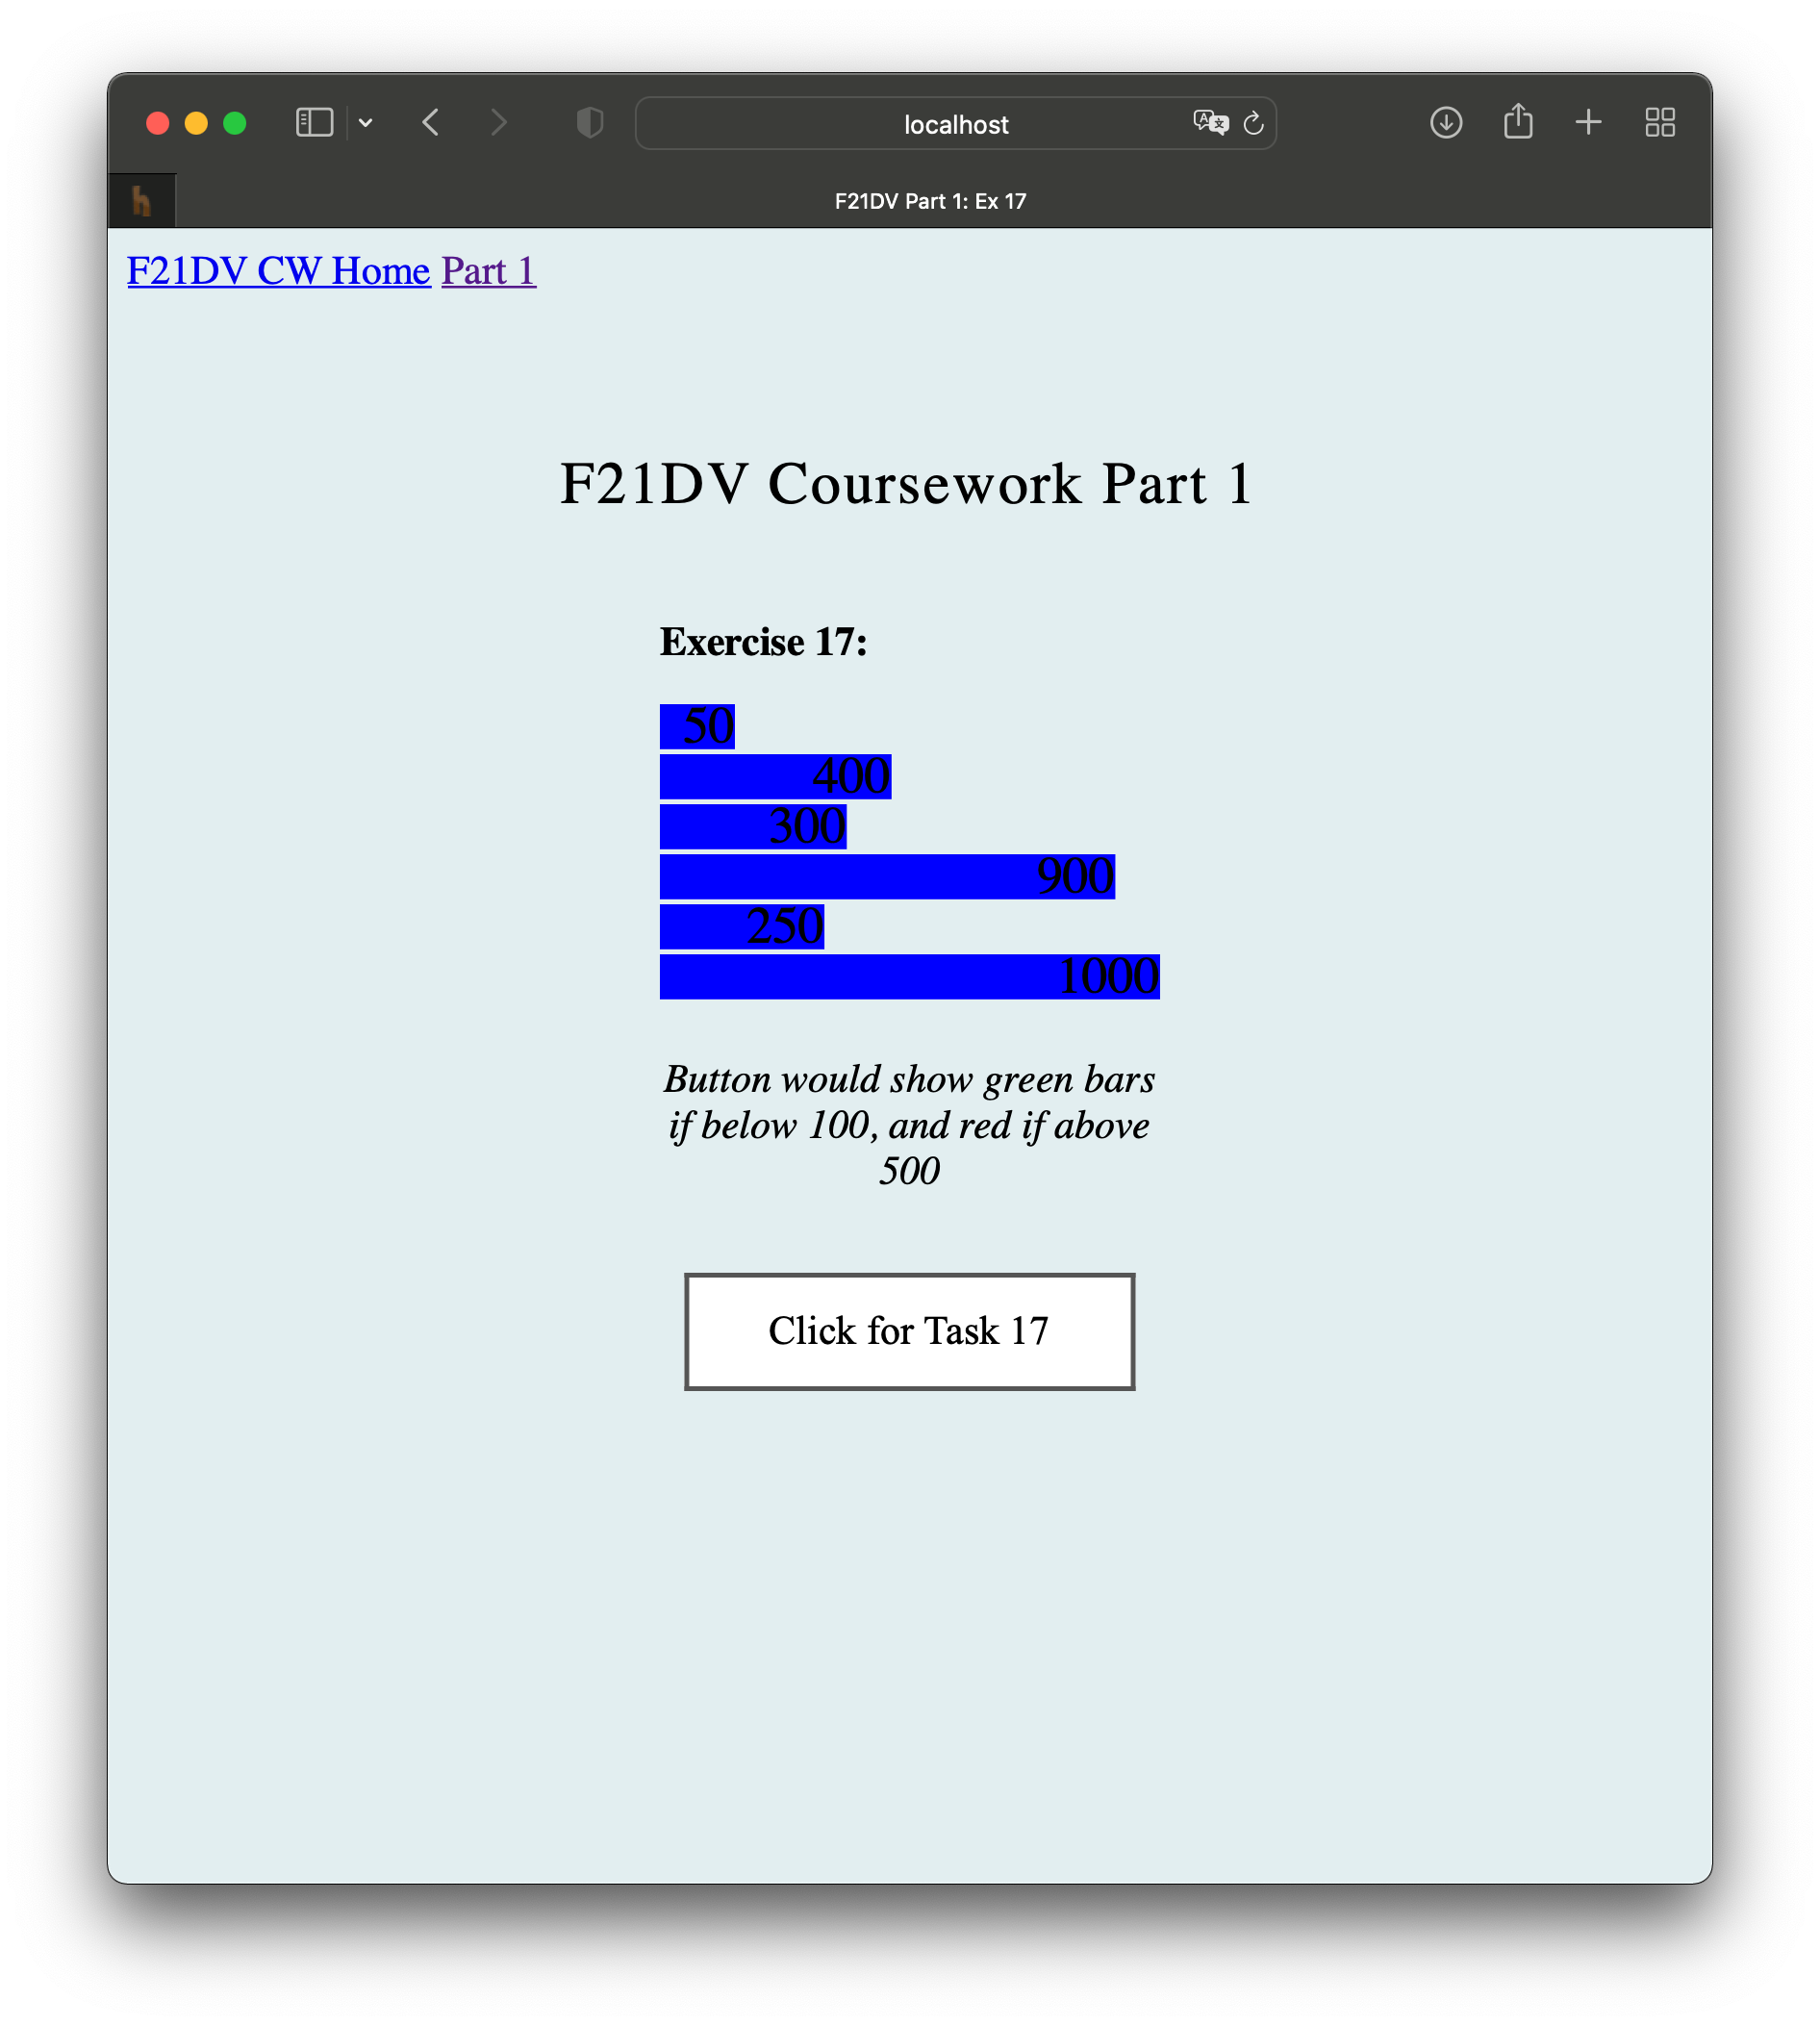
\includegraphics[width = 8cm]{images/ex17_1.png}
    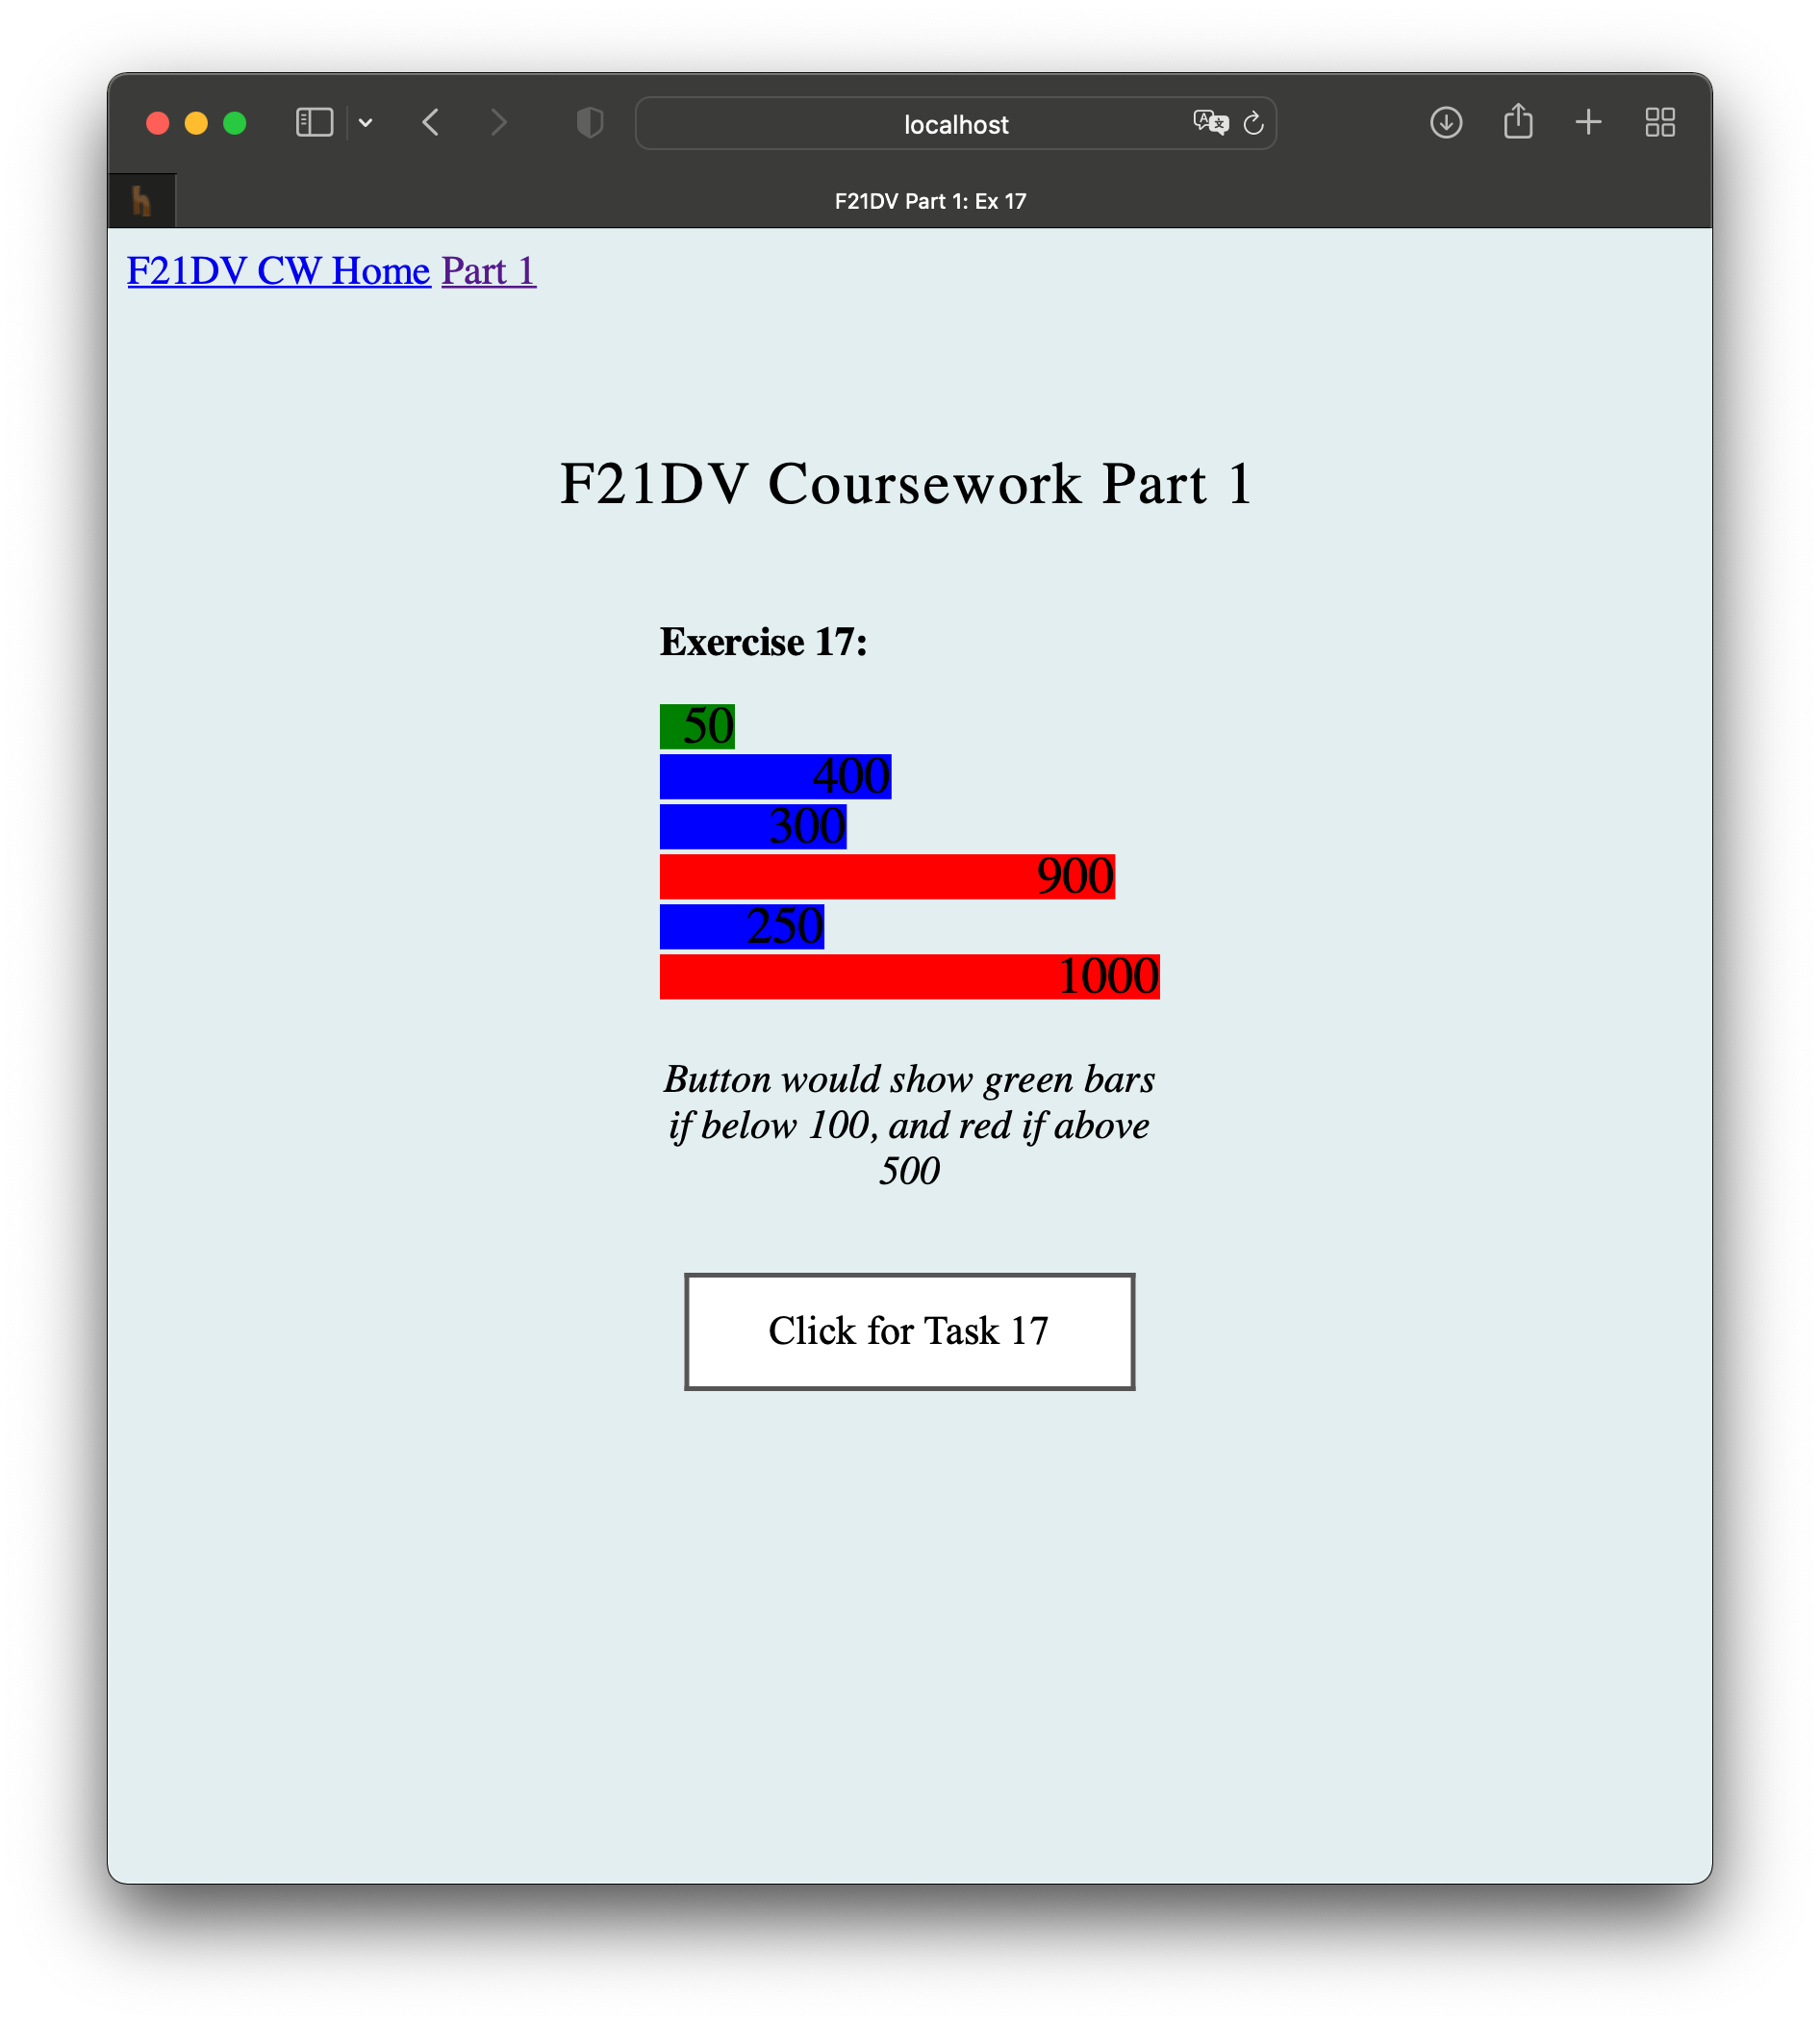
\includegraphics[width = 8cm]{images/ex17_2.png}
    \label{fig:ex17}
    \caption{Exercise 17}
\end{figure}
\FloatBarrier
% \lstinputlisting[language=JavaScript]{../../public/js/part1/task17.js}
Exercise 17 is just a simple horizontal bar chart, like the example from Exercise 14 and 15. We first
create an svg, and then slowly add rectangles onto it, and aligning it using transform-translations.
The button then changes the colour of the rectangles depending on the value. 

\newpage
\section{Exercise 18 \& 19}
\begin{figure}[!ht]
    \centering
    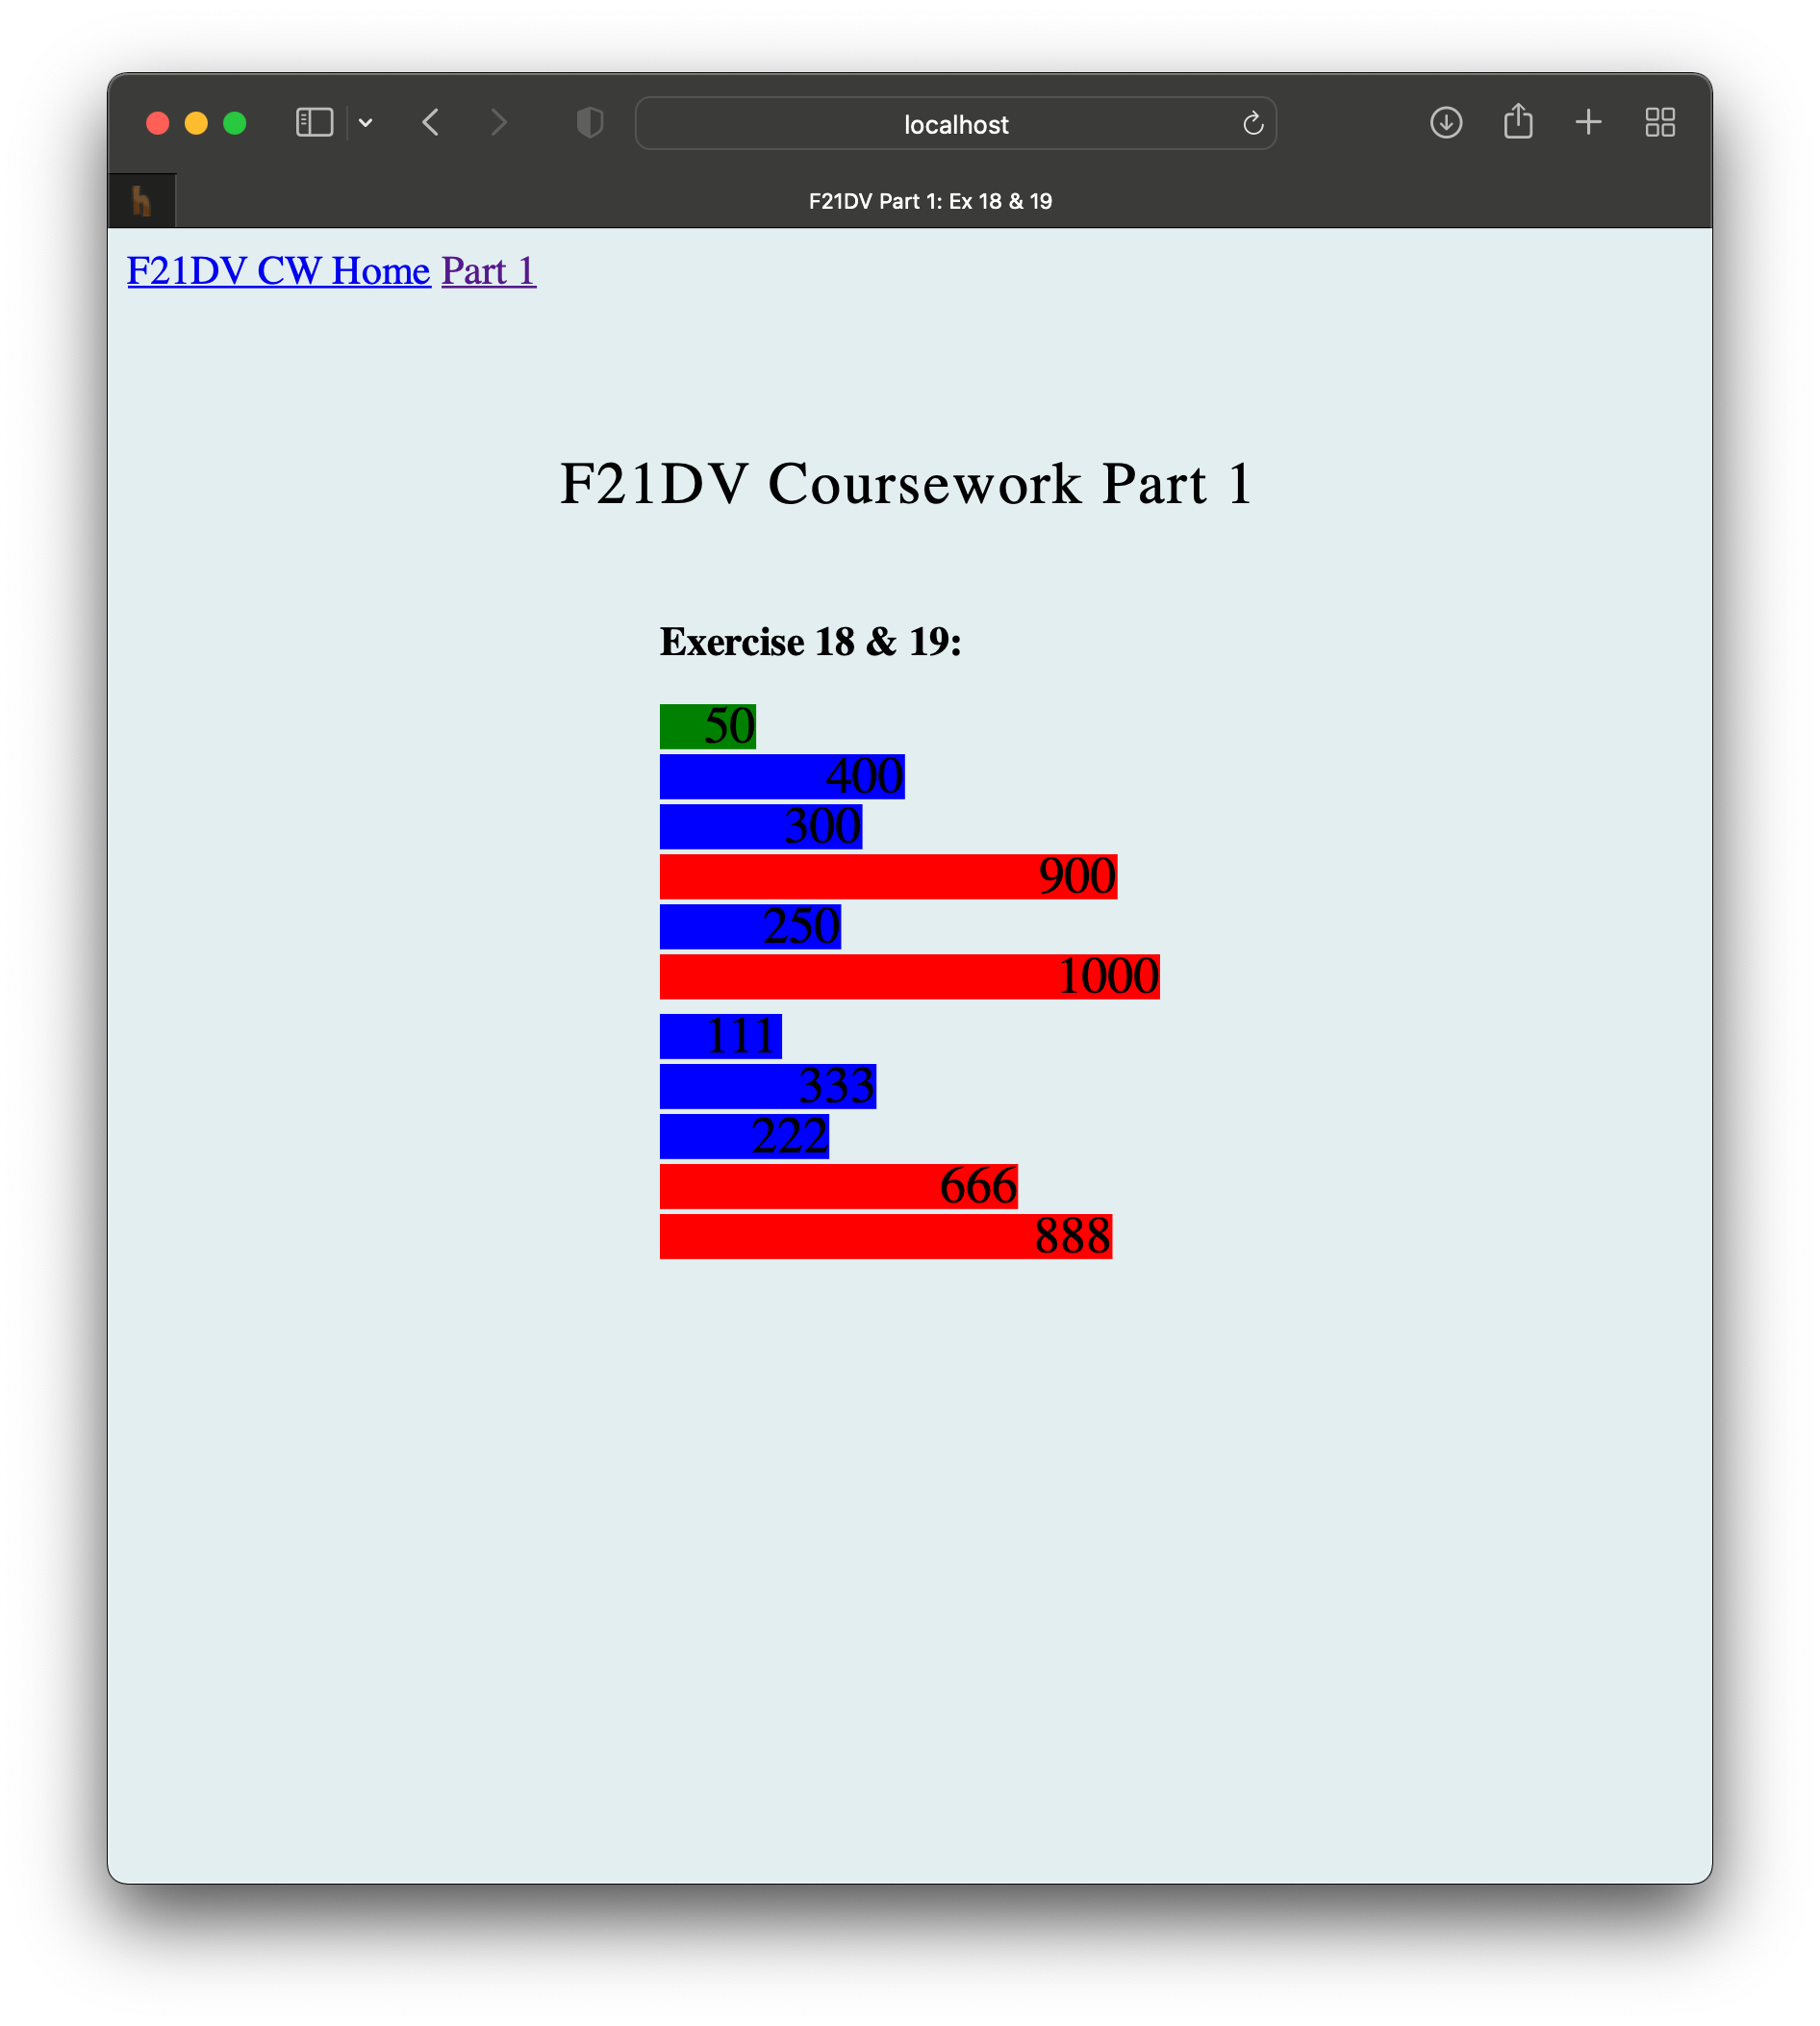
\includegraphics[width = 8cm]{images/ex18.png}
    \label{fig:ex18}
    \caption{Exercise 18 \& 19}
\end{figure}
\FloatBarrier
\lstinputlisting[language=JavaScript]{../../public/js/part1/task18n19.js}
Exercise 18 is plotting some bar charts based off some csv data, and question 19 extends that by adding
them all into a function so that the function could be called as many times as desired, and with different
data each time. The function would append a new SVG to the \verb|.answerCenter| div each time the function
is called, and then rectangles would be added onto it afterwards.

\newpage
\section{Exercise 20}
\begin{figure}[!ht]
    \centering
    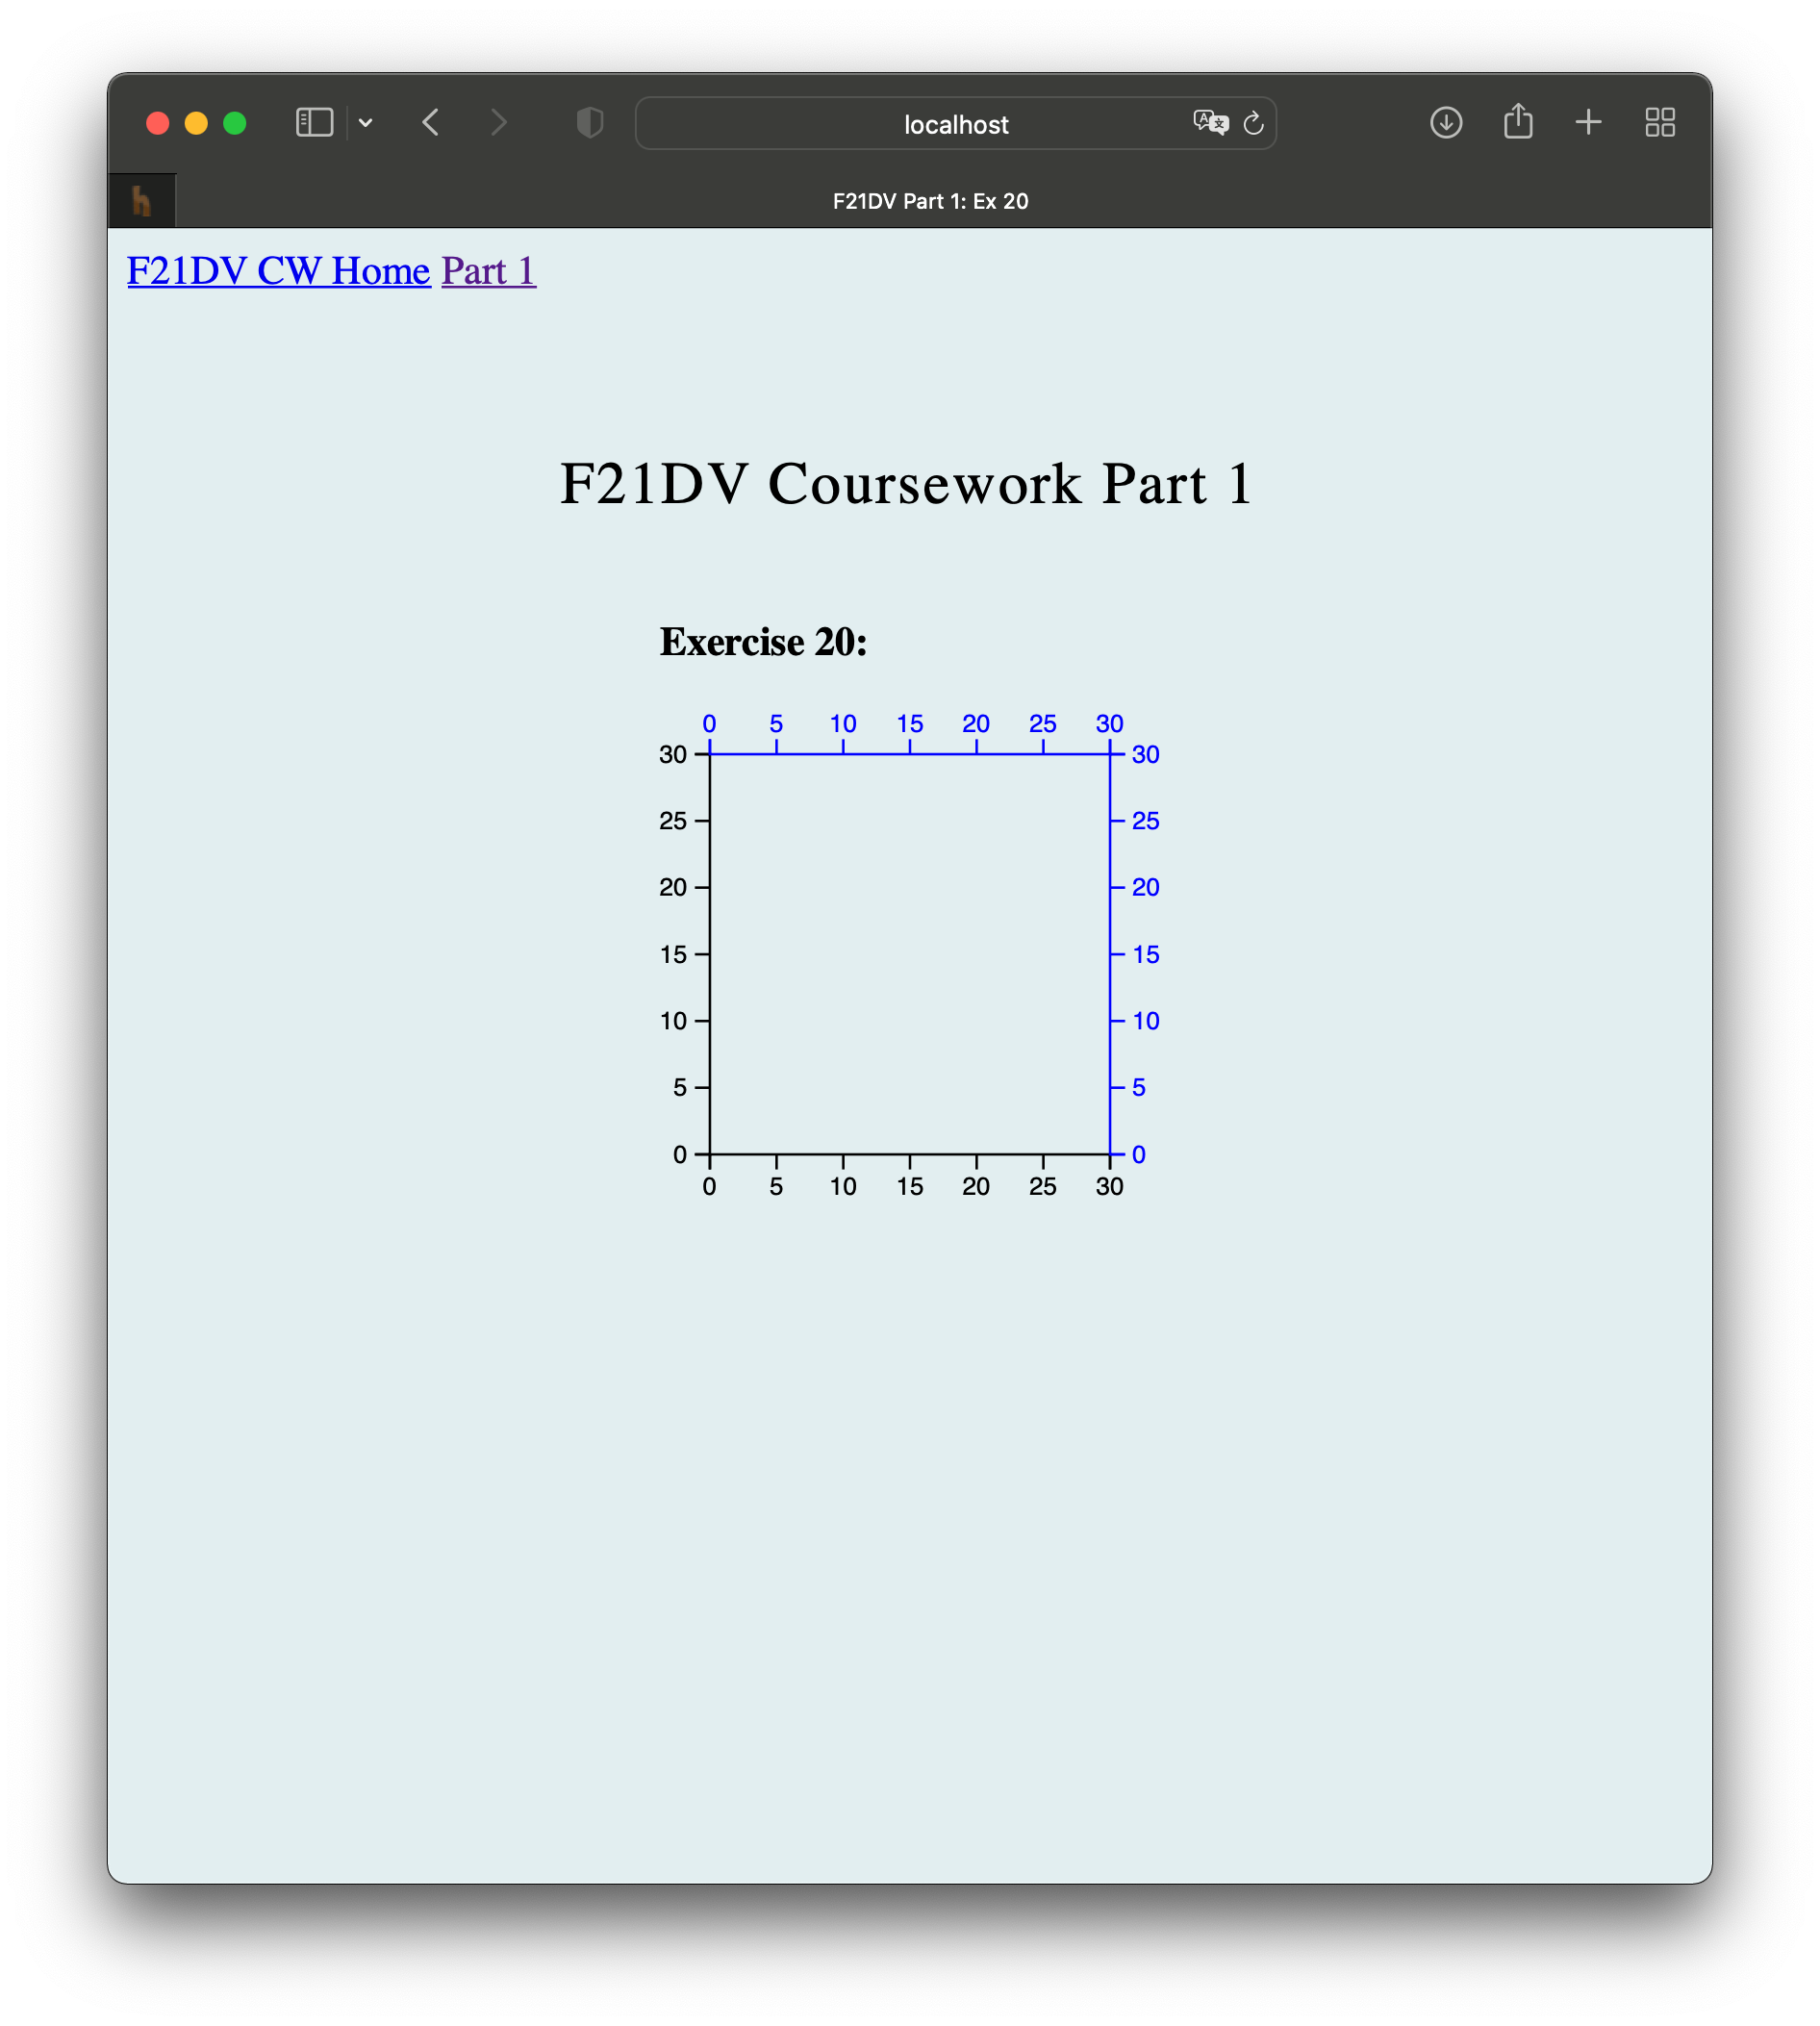
\includegraphics[width = 8cm]{images/ex20.png}
    \label{fig:ex20}
    \caption{Exercise 20}
\end{figure}
\FloatBarrier
% \lstinputlisting[language=JavaScript]{../../public/js/part1/task18n19.js}
Exercise 20 is just the same as plotting the axes in exercise 14 and 15. The only difference is the two 
more top and right axis that needs to be plot. This would just have a different \verb|.style()| colour,
and also differnt transform-translation values.

\newpage
\section{Exercise 21}
\begin{figure}[!ht]
    \centering
    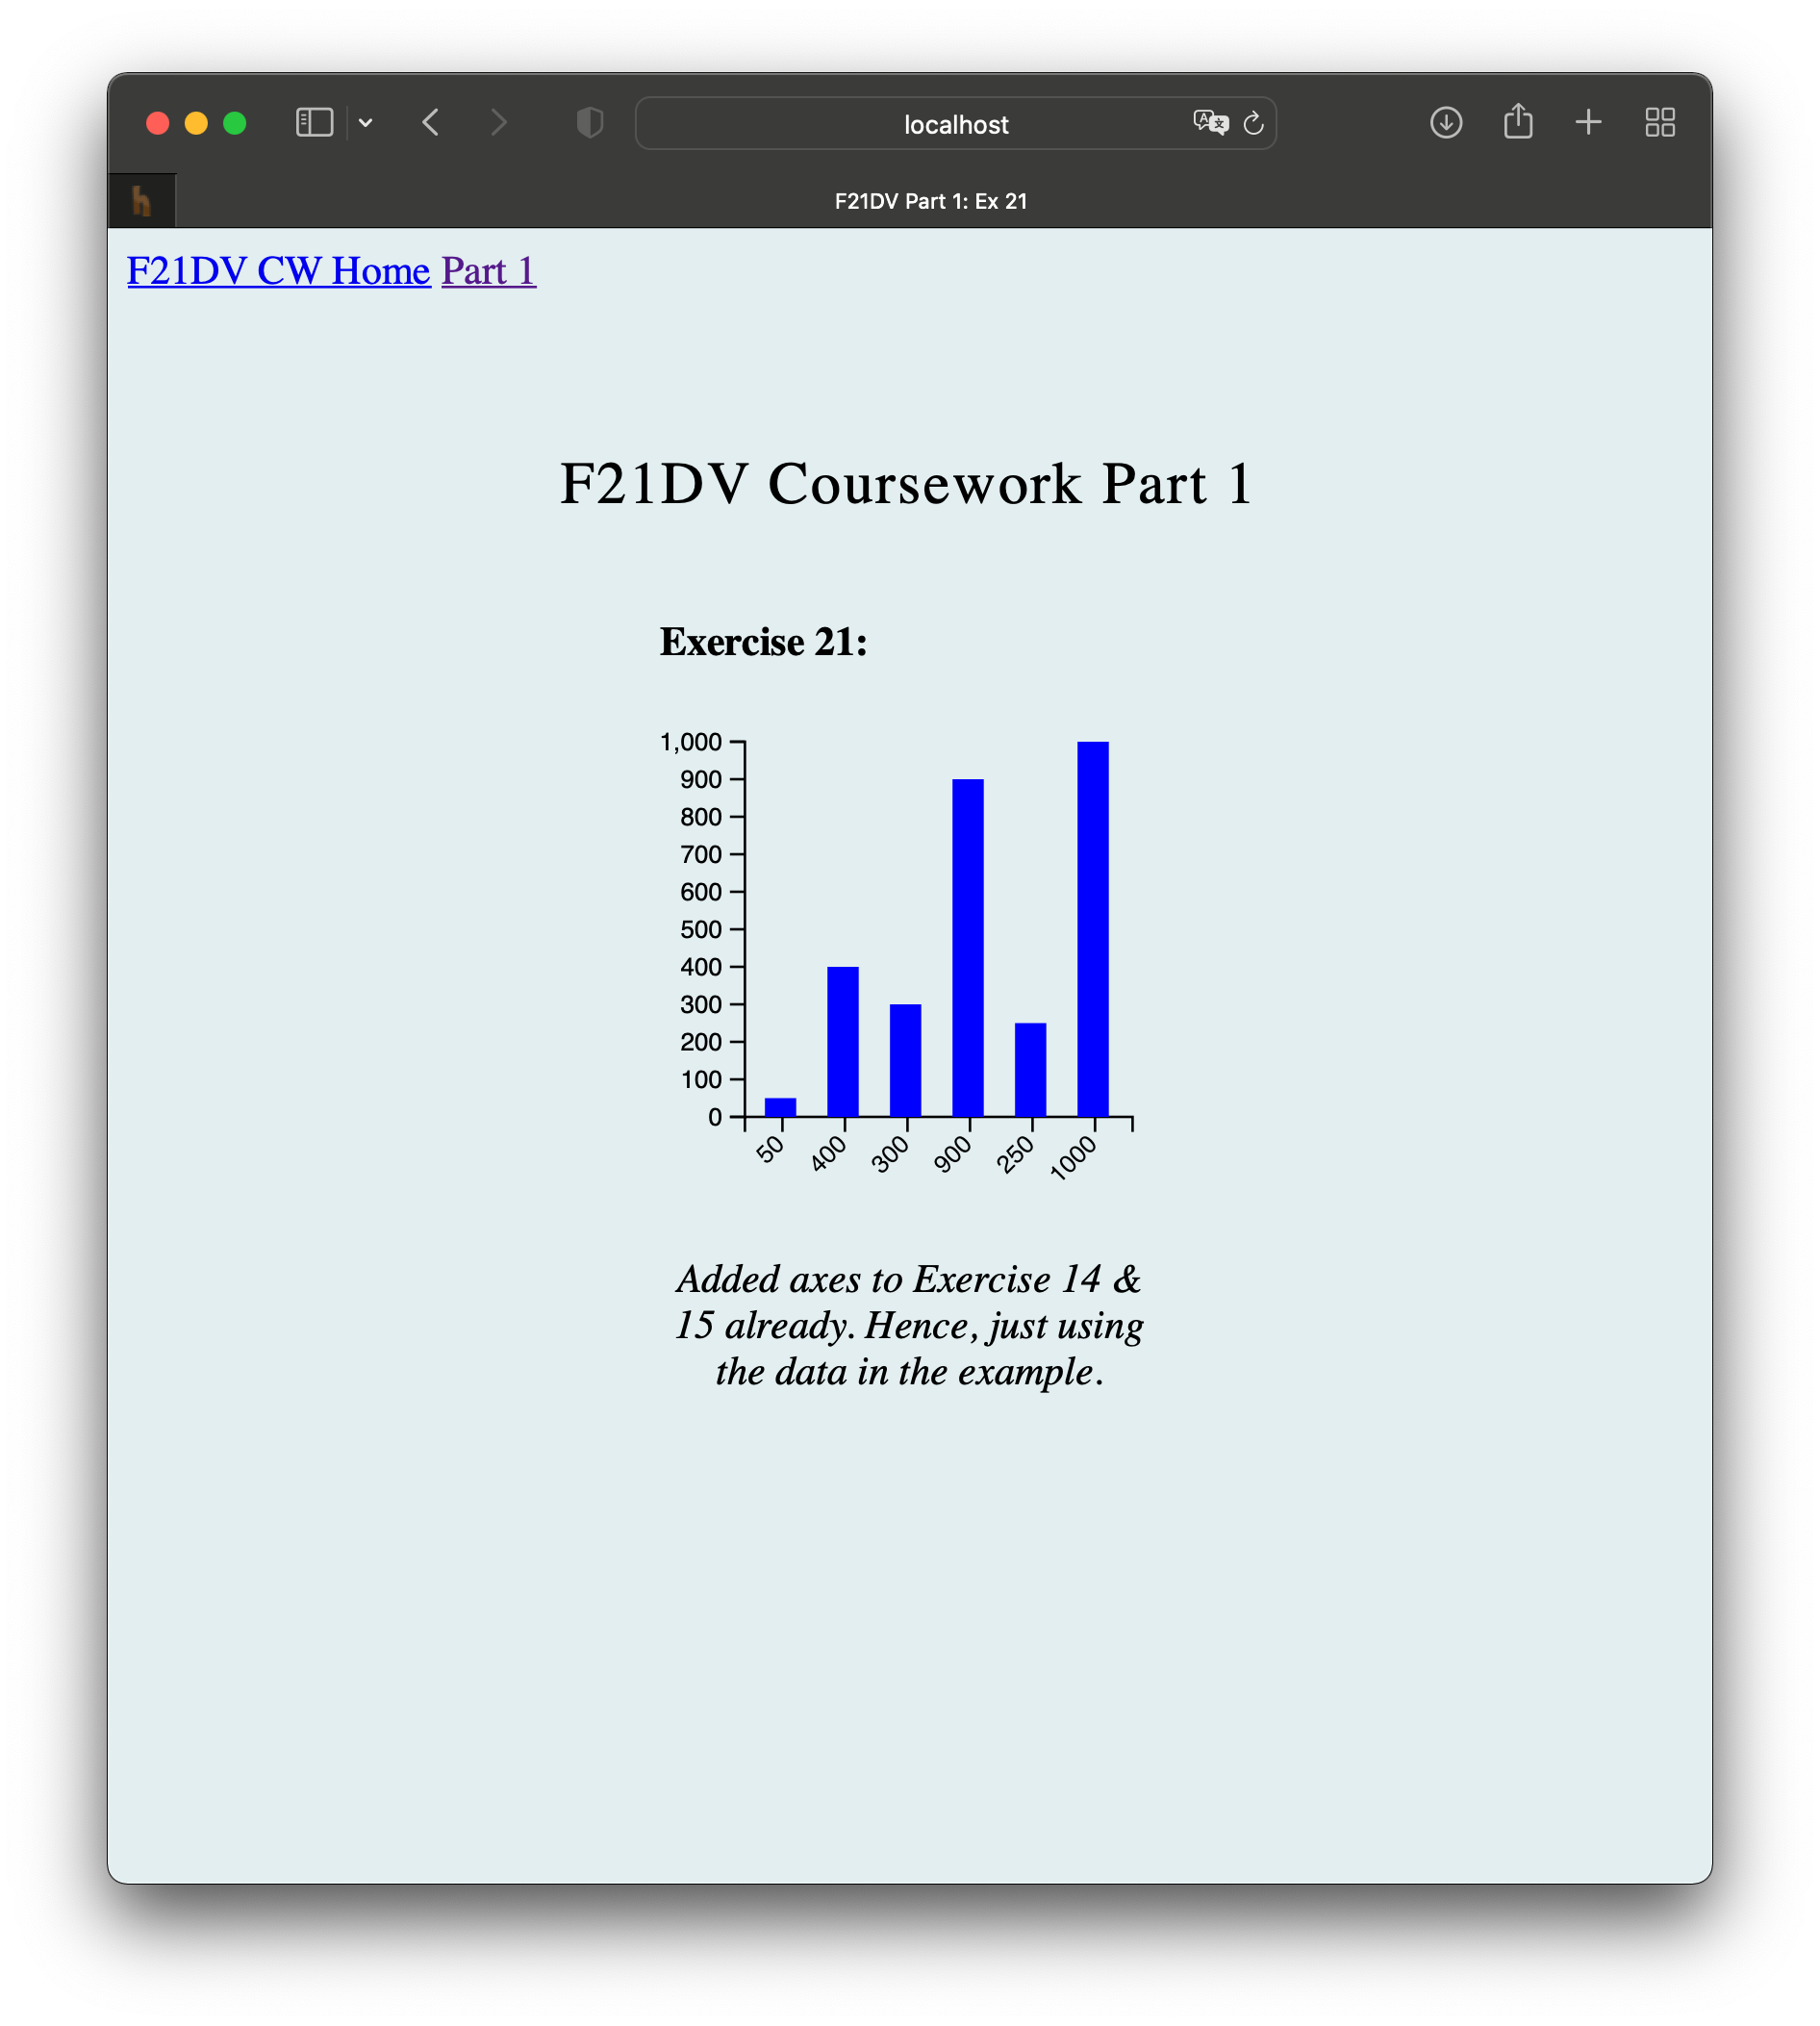
\includegraphics[width = 8cm]{images/ex21.png}
    \label{fig:ex21}
    \caption{Exercise 21}
\end{figure}
\FloatBarrier
% \lstinputlisting[language=JavaScript]{../../public/js/part1/task18n19.js}
What was requested in exercise 21 was done in exercise 14 and 15, hence just using different data values 
from the example given for this. 

\newpage
\section{Exercise 22}
\lstinputlisting[language=JavaScript]{../../public/js/part1/task22.js}
Task 22 has no output as its sole purpose is to provide generalised functions for the remaining questions.
Its main functions includes:
\begin{itemize}
    \item \verb|createSvg()| | which creates the svg element, and returns the svg itself, horizontal scale,
    and verticle scale.
    \item \verb|addLines()| | which takes the createSvg() from before, and uses either its svg, hor/vertical
    scale, and processes some lines and adds to it.
    \item \verb|addLinesShape()| | same as before, just this time having and extra function that adds
    data points based on the lines to add. 
    \item \verb|addLinesCoor()| | extends \verb|addLinesShape()| and adds coordinates near the data points
    along the lines. Users can self identify which points to add.
    \item \verb|addLinesShapeDifferentColor()| | adds lines and data points (of different shape), just that
    this time, the colour of data points is dependant on the data value.
\end{itemize}

\newpage
\section{Exercise 23}
\begin{figure}[!ht]
    \centering
    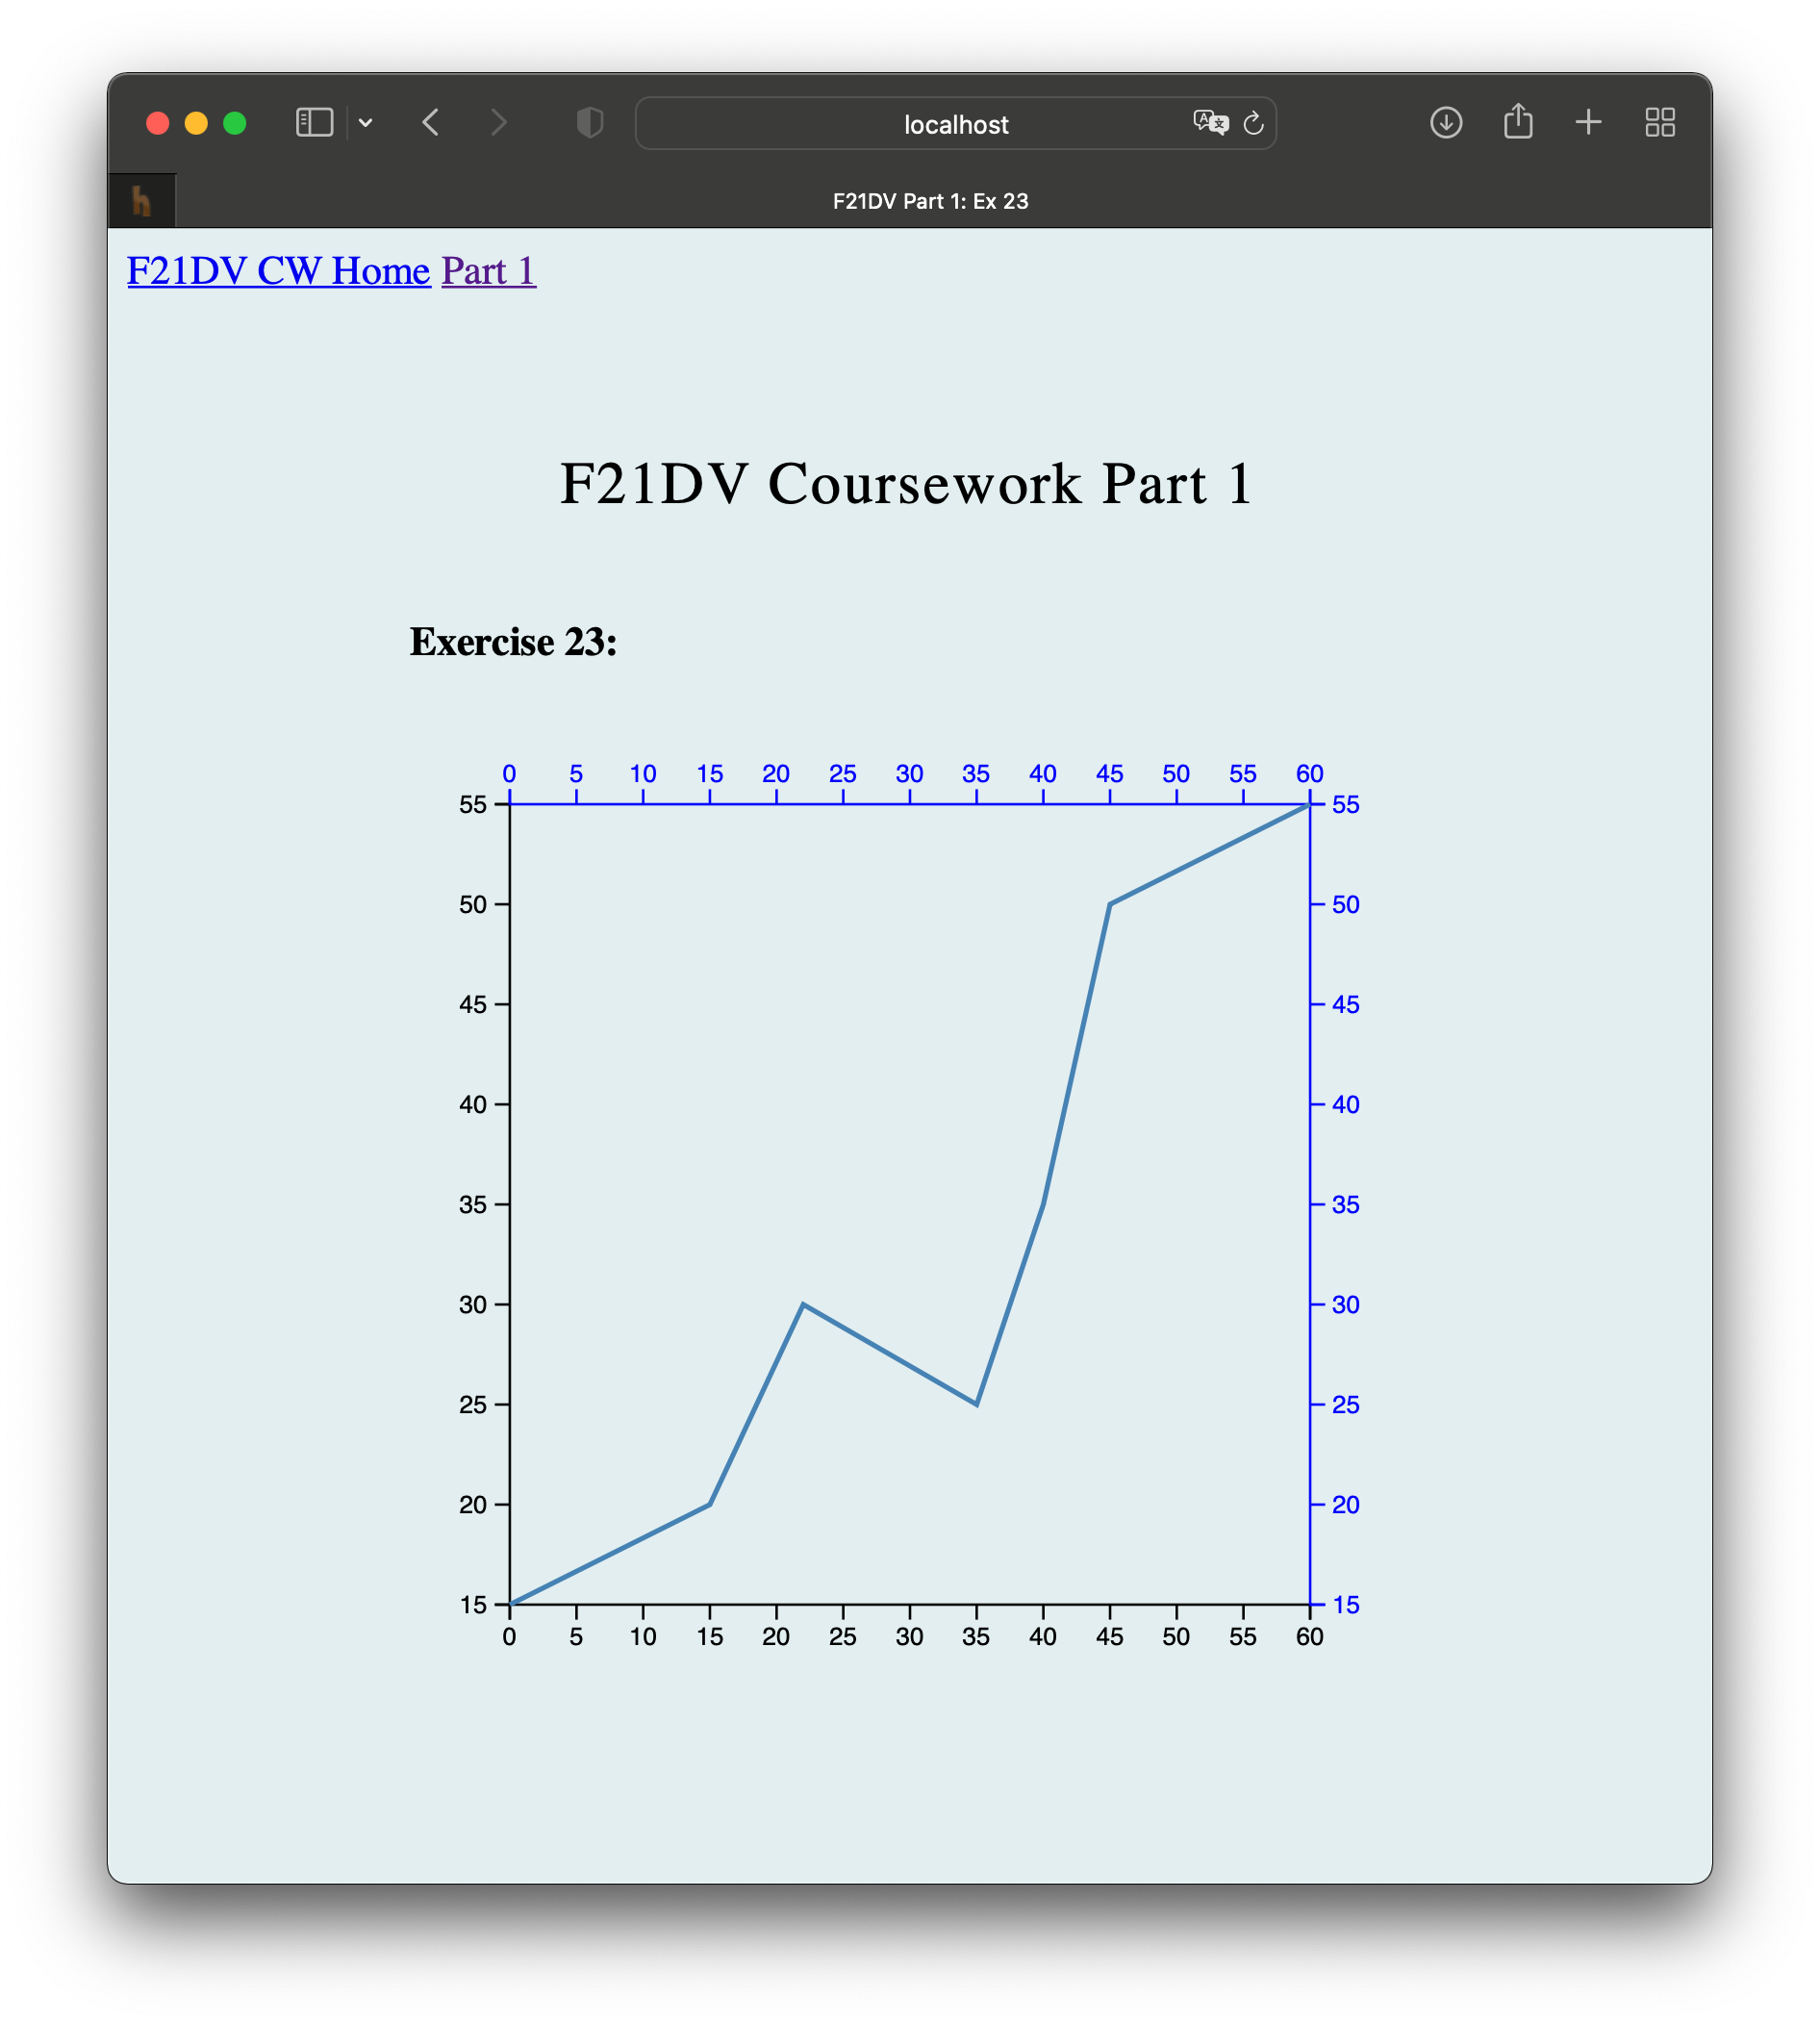
\includegraphics[width = 8cm]{images/ex23.png}
    \label{fig:ex23}
    \caption{Exercise 23}
\end{figure}
\FloatBarrier
\lstinputlisting[language=JavaScript]{../../public/js/part1/task23.js}
Exercise 23 reads data containing x, y coordinates from a csv file, and plot these on the svg element
using the \verb|createSVG()| and \verb|addLines()| function imported from \verb|task22.js|.

\newpage
\section{Exercise 24}
\begin{figure}[!ht]
    \centering
    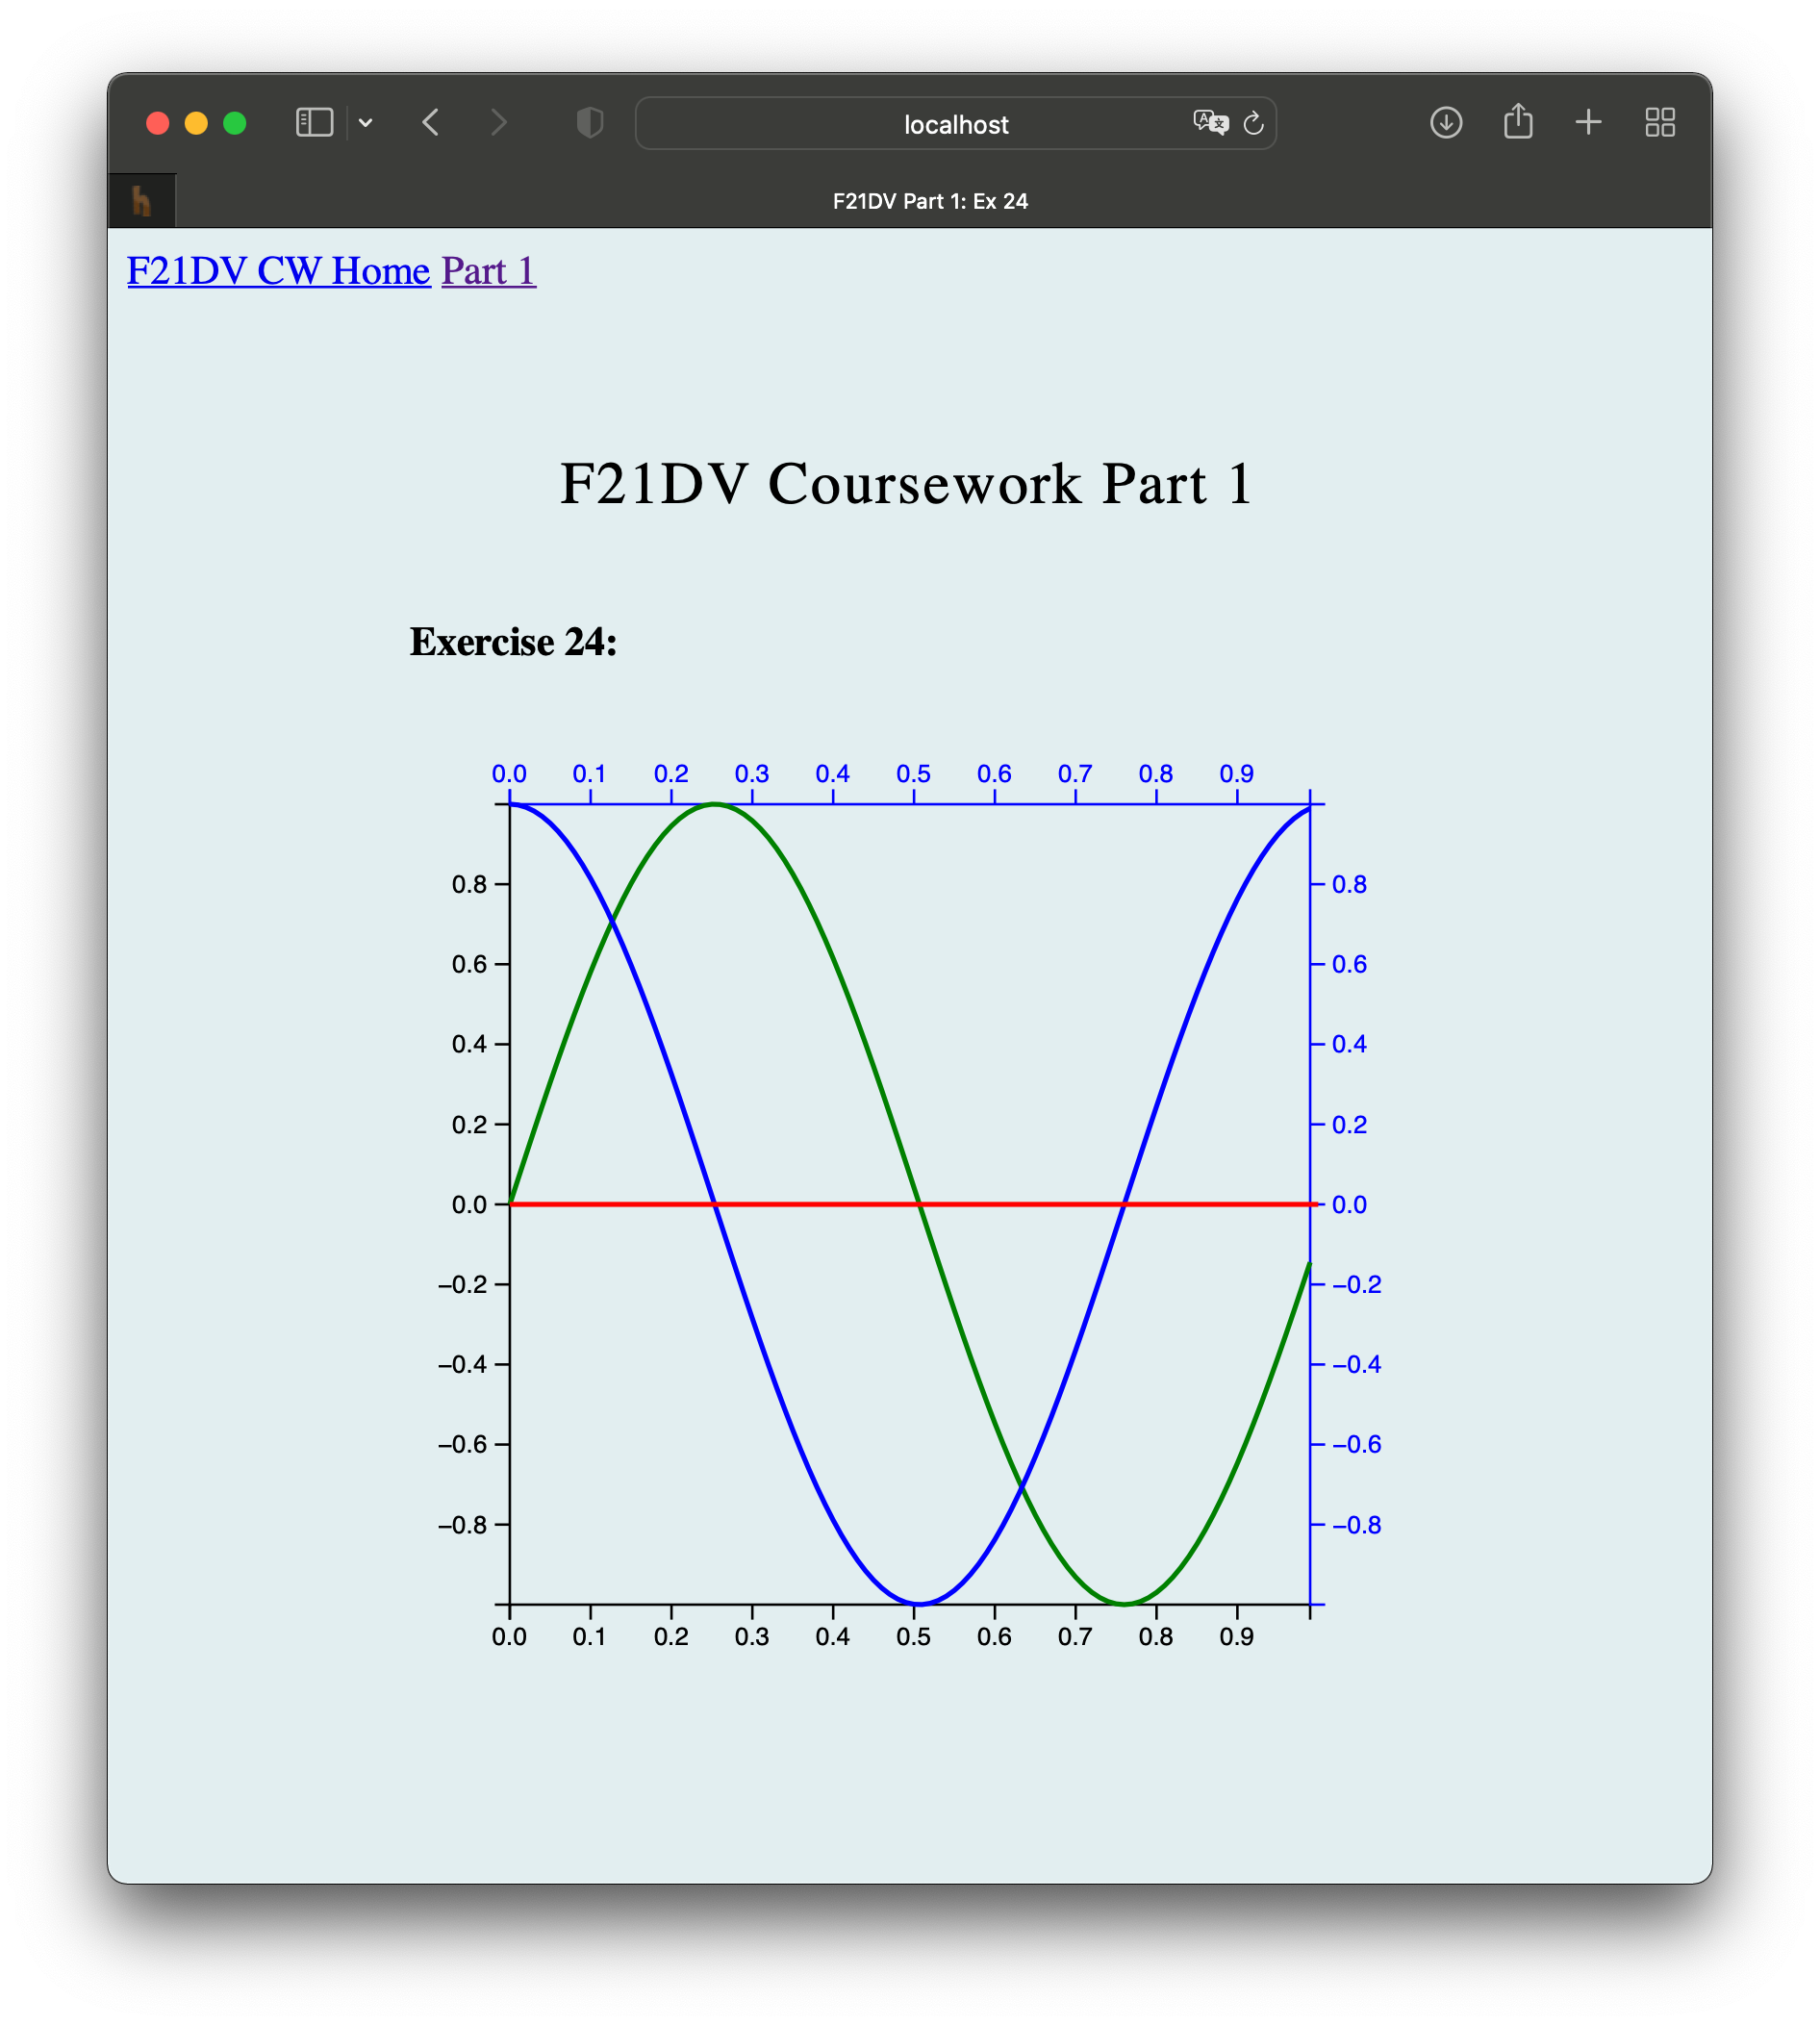
\includegraphics[width = 8cm]{images/ex24.png}
    \label{fig:ex24}
    \caption{Exercise 24}
\end{figure}
\FloatBarrier
\lstinputlisting[language=JavaScript]{../../public/js/part1/task24.js}
Same as exercise 22. The difference is just with the self generated sine and cos data points. Once 
generated, the sine and cosine lines are added, and I added a X axis red line just to  show the x axis. 

\newpage
\section{Exercise 25 to 27}
\begin{figure}[!ht]
    \centering
    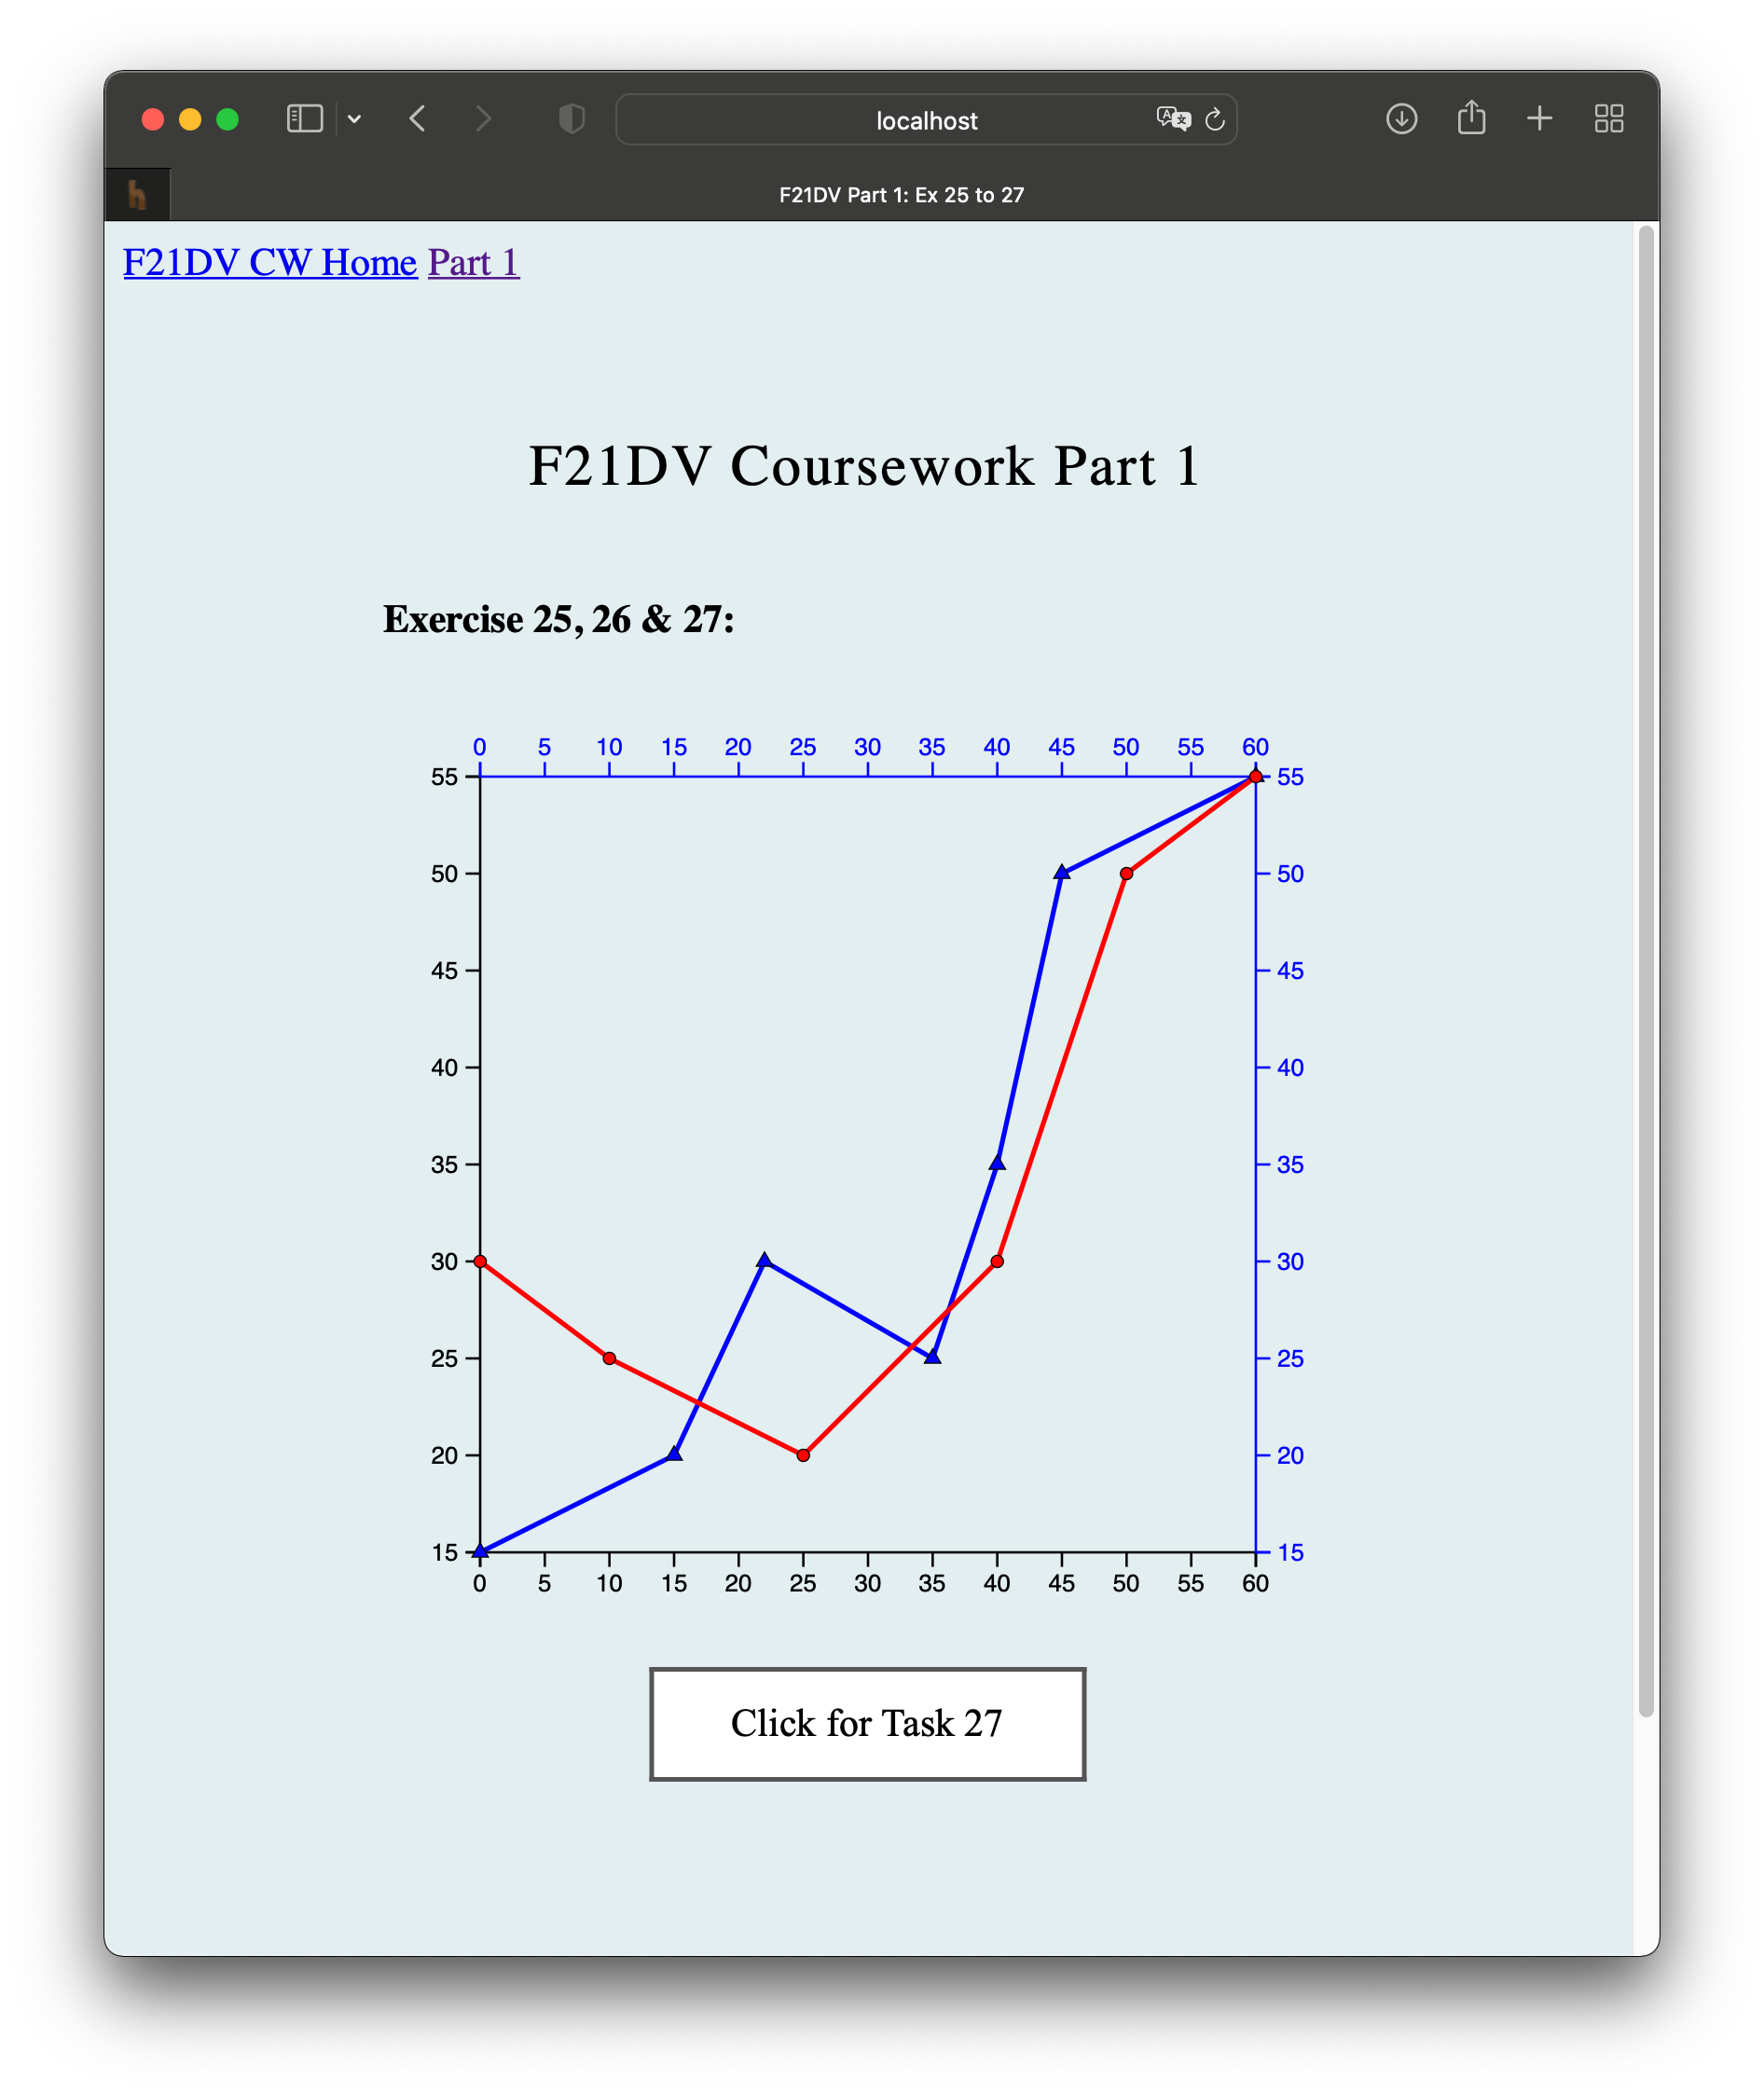
\includegraphics[width = 8cm]{images/ex25_1.png}
    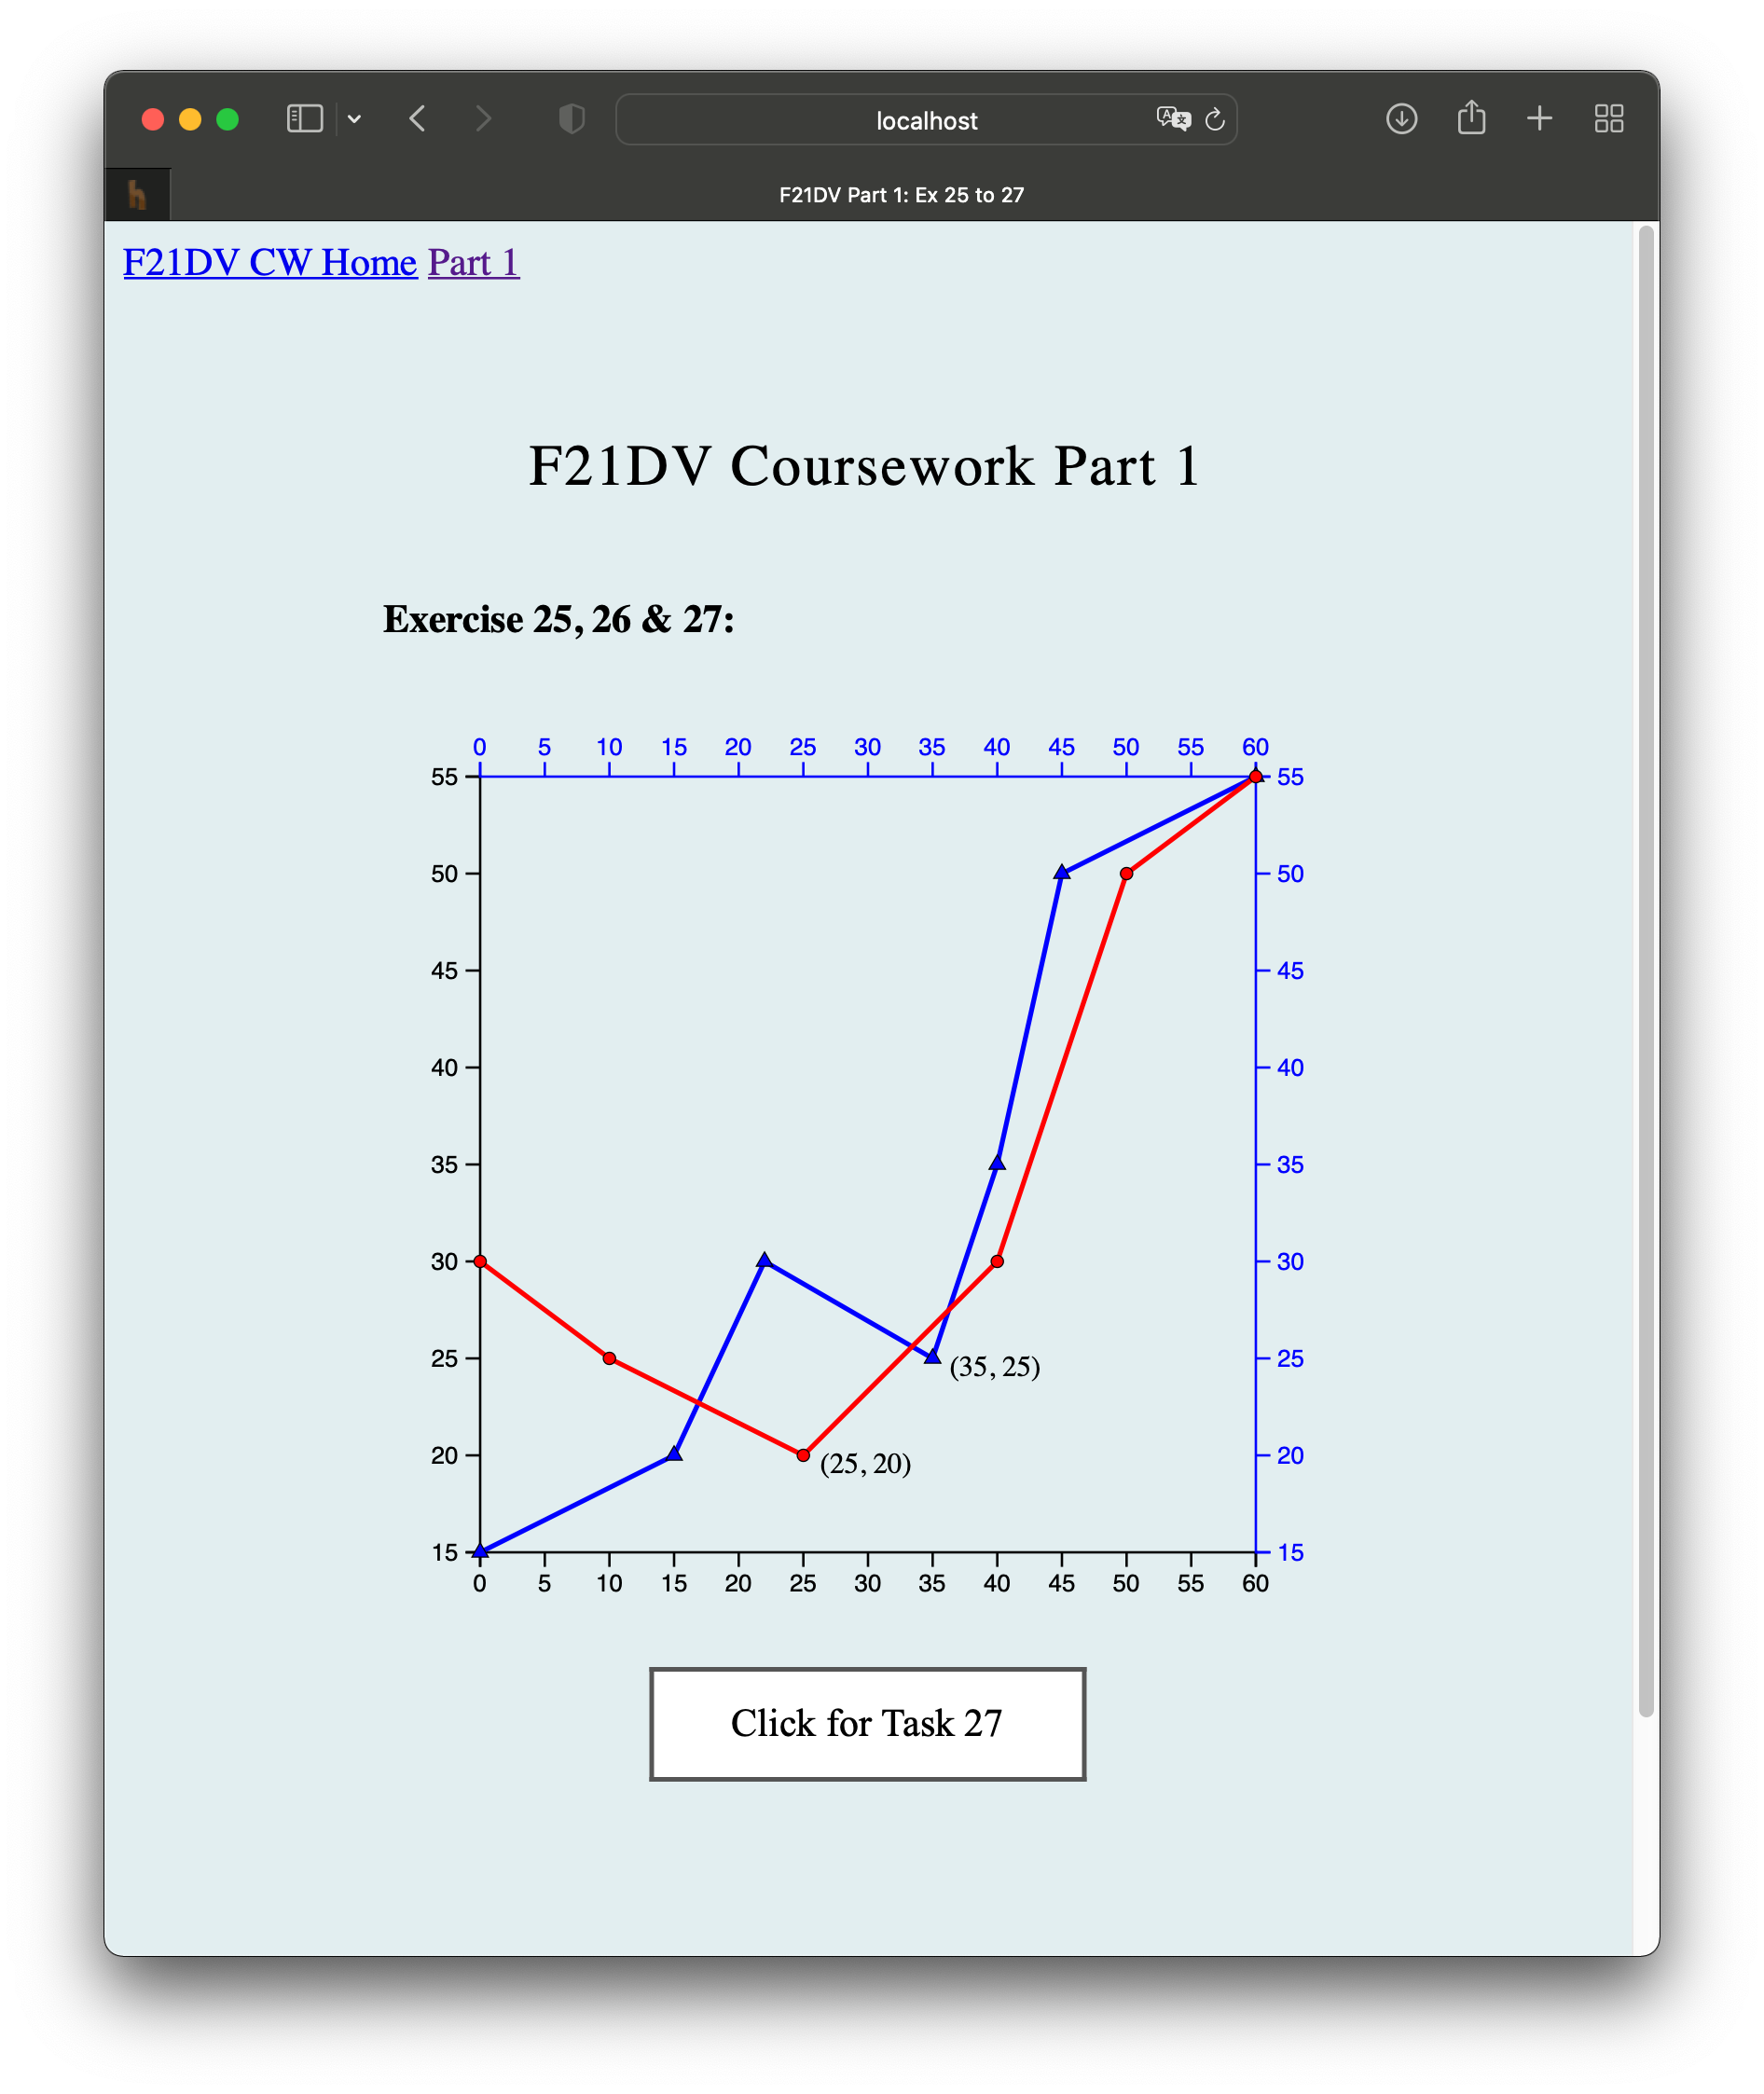
\includegraphics[width = 8cm]{images/ex25_2.png}
    \label{fig:ex25}
    \caption{Exercise 25 to 27}
\end{figure}
\FloatBarrier
\lstinputlisting[language=JavaScript]{../../public/js/part1/task25to27.js}
I have decided to combine exercises 25 and 26, since they are essentially the same thing just with a 
different shape. Making use of the function \verb|addLinesShape()| from \verb|task22.js|, we simply call
the function twice. \\
\par For the task in exercise 27 however, I have decided to use a button to complete this. Uppon the
press of the button, we add a point to each graph using the \verb|addLinesCoor()| function, and we define
the index of the data point we would like to plot. For instance, I plot the 3rd index for the blue line,
and the 2nd index for the red line.

\newpage
\section{Exercise 28}
\begin{figure}[!ht]
    \centering
    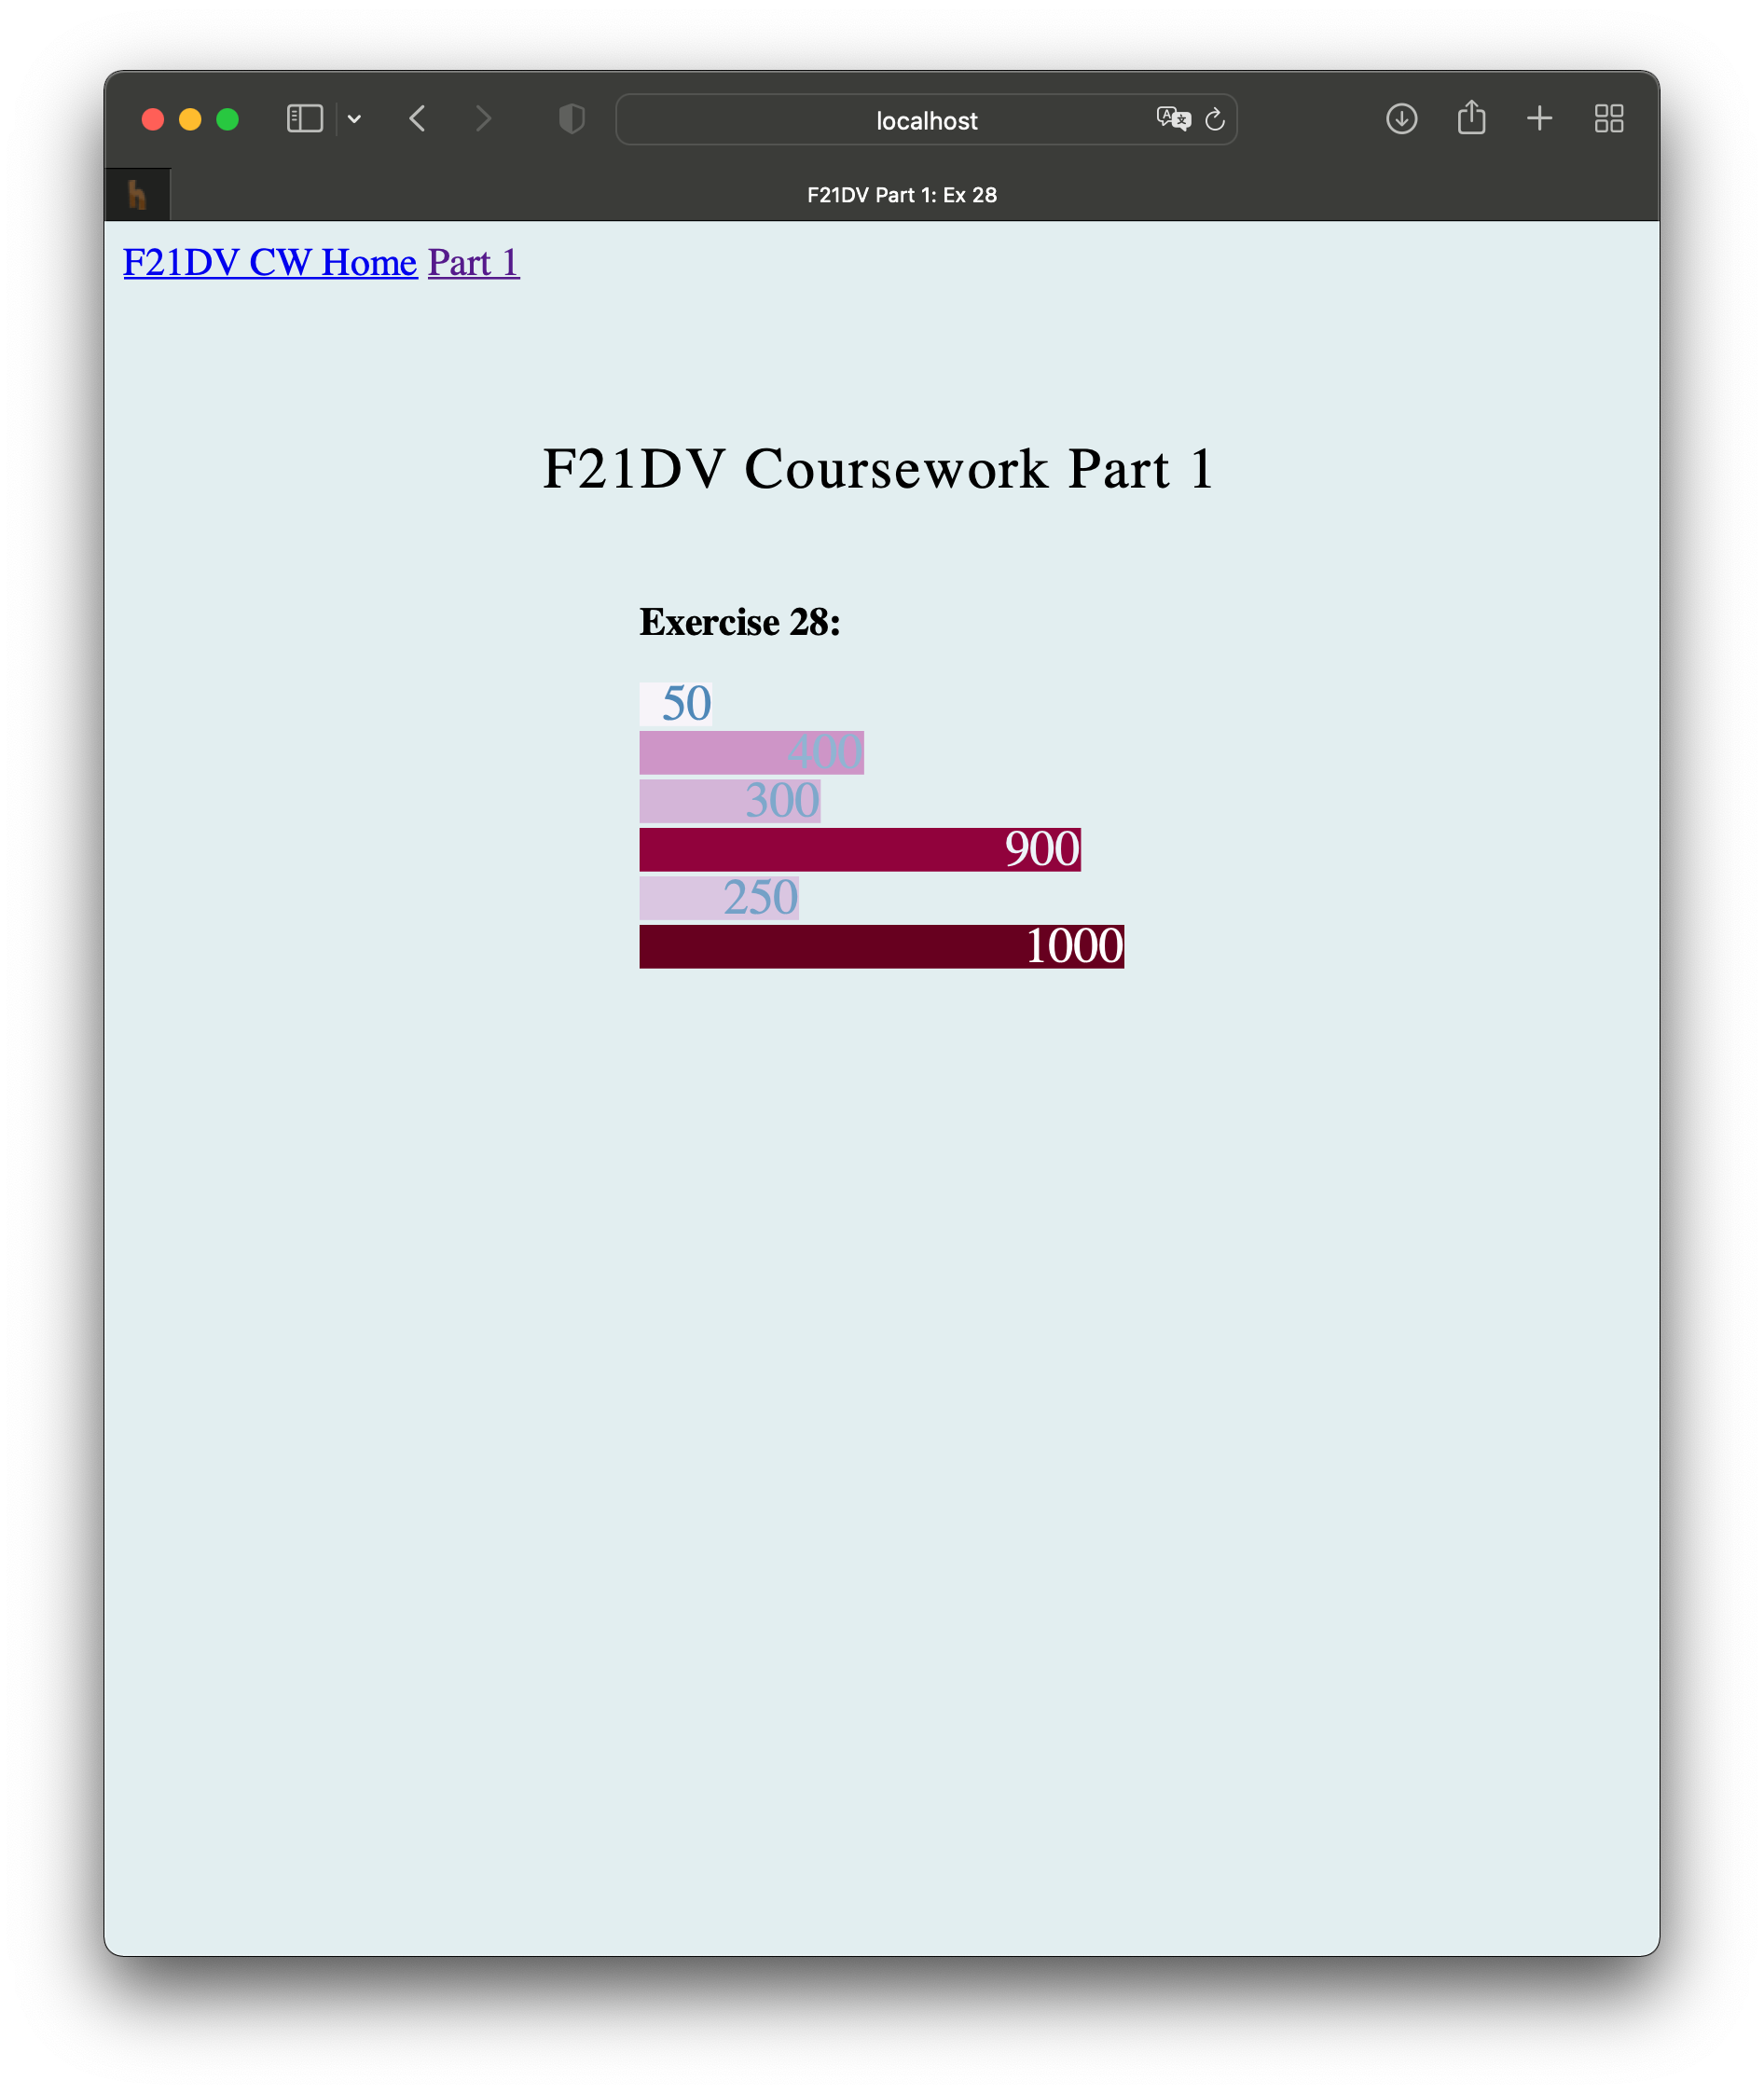
\includegraphics[width = 8cm]{images/ex28.png}
    \label{fig:ex28}
    \caption{Exercise 28}
\end{figure}
\begin{lstlisting}[language=JavaScript,
    caption={abstract from task28.js},
    captionpos=b,
    label={lst:ex28}]
    ...
    // Colour Scale.
    const boxCol = d3.scaleSequential()
                        .domain(d3.extent(data))
                        .interpolator(d3.interpolatePuRd);
    const textCol = d3.interpolateRgb('steelblue', 'white');
    
    // Add 'rect' elements.
    g.append('rect')
        .attr('width', d => xScale(d))
        .attr('height', barHeight - margin)
        .attr('fill', d => boxCol(d));
    
    // Add text object to rectangle.
    g.append('text')
        .attr('x', d => xScale(d))
        .attr('y', barHeight/2)
        .attr('dy', '.25em')
        .style('text-anchor', 'end')
        .text(d => d)
        .style('fill', d => textCol(d/1000));
    ...
\end{lstlisting}
Exercise 28 is the same as what that was done in exercise 17. The only difference is with the definition
of the colour schemes, as shown in listing \ref{lst:ex28}. Then using the scale, we obtain the colours
for each rectangle.

\newpage
\section{Exercise 29}
\begin{figure}[!ht]
    \centering
    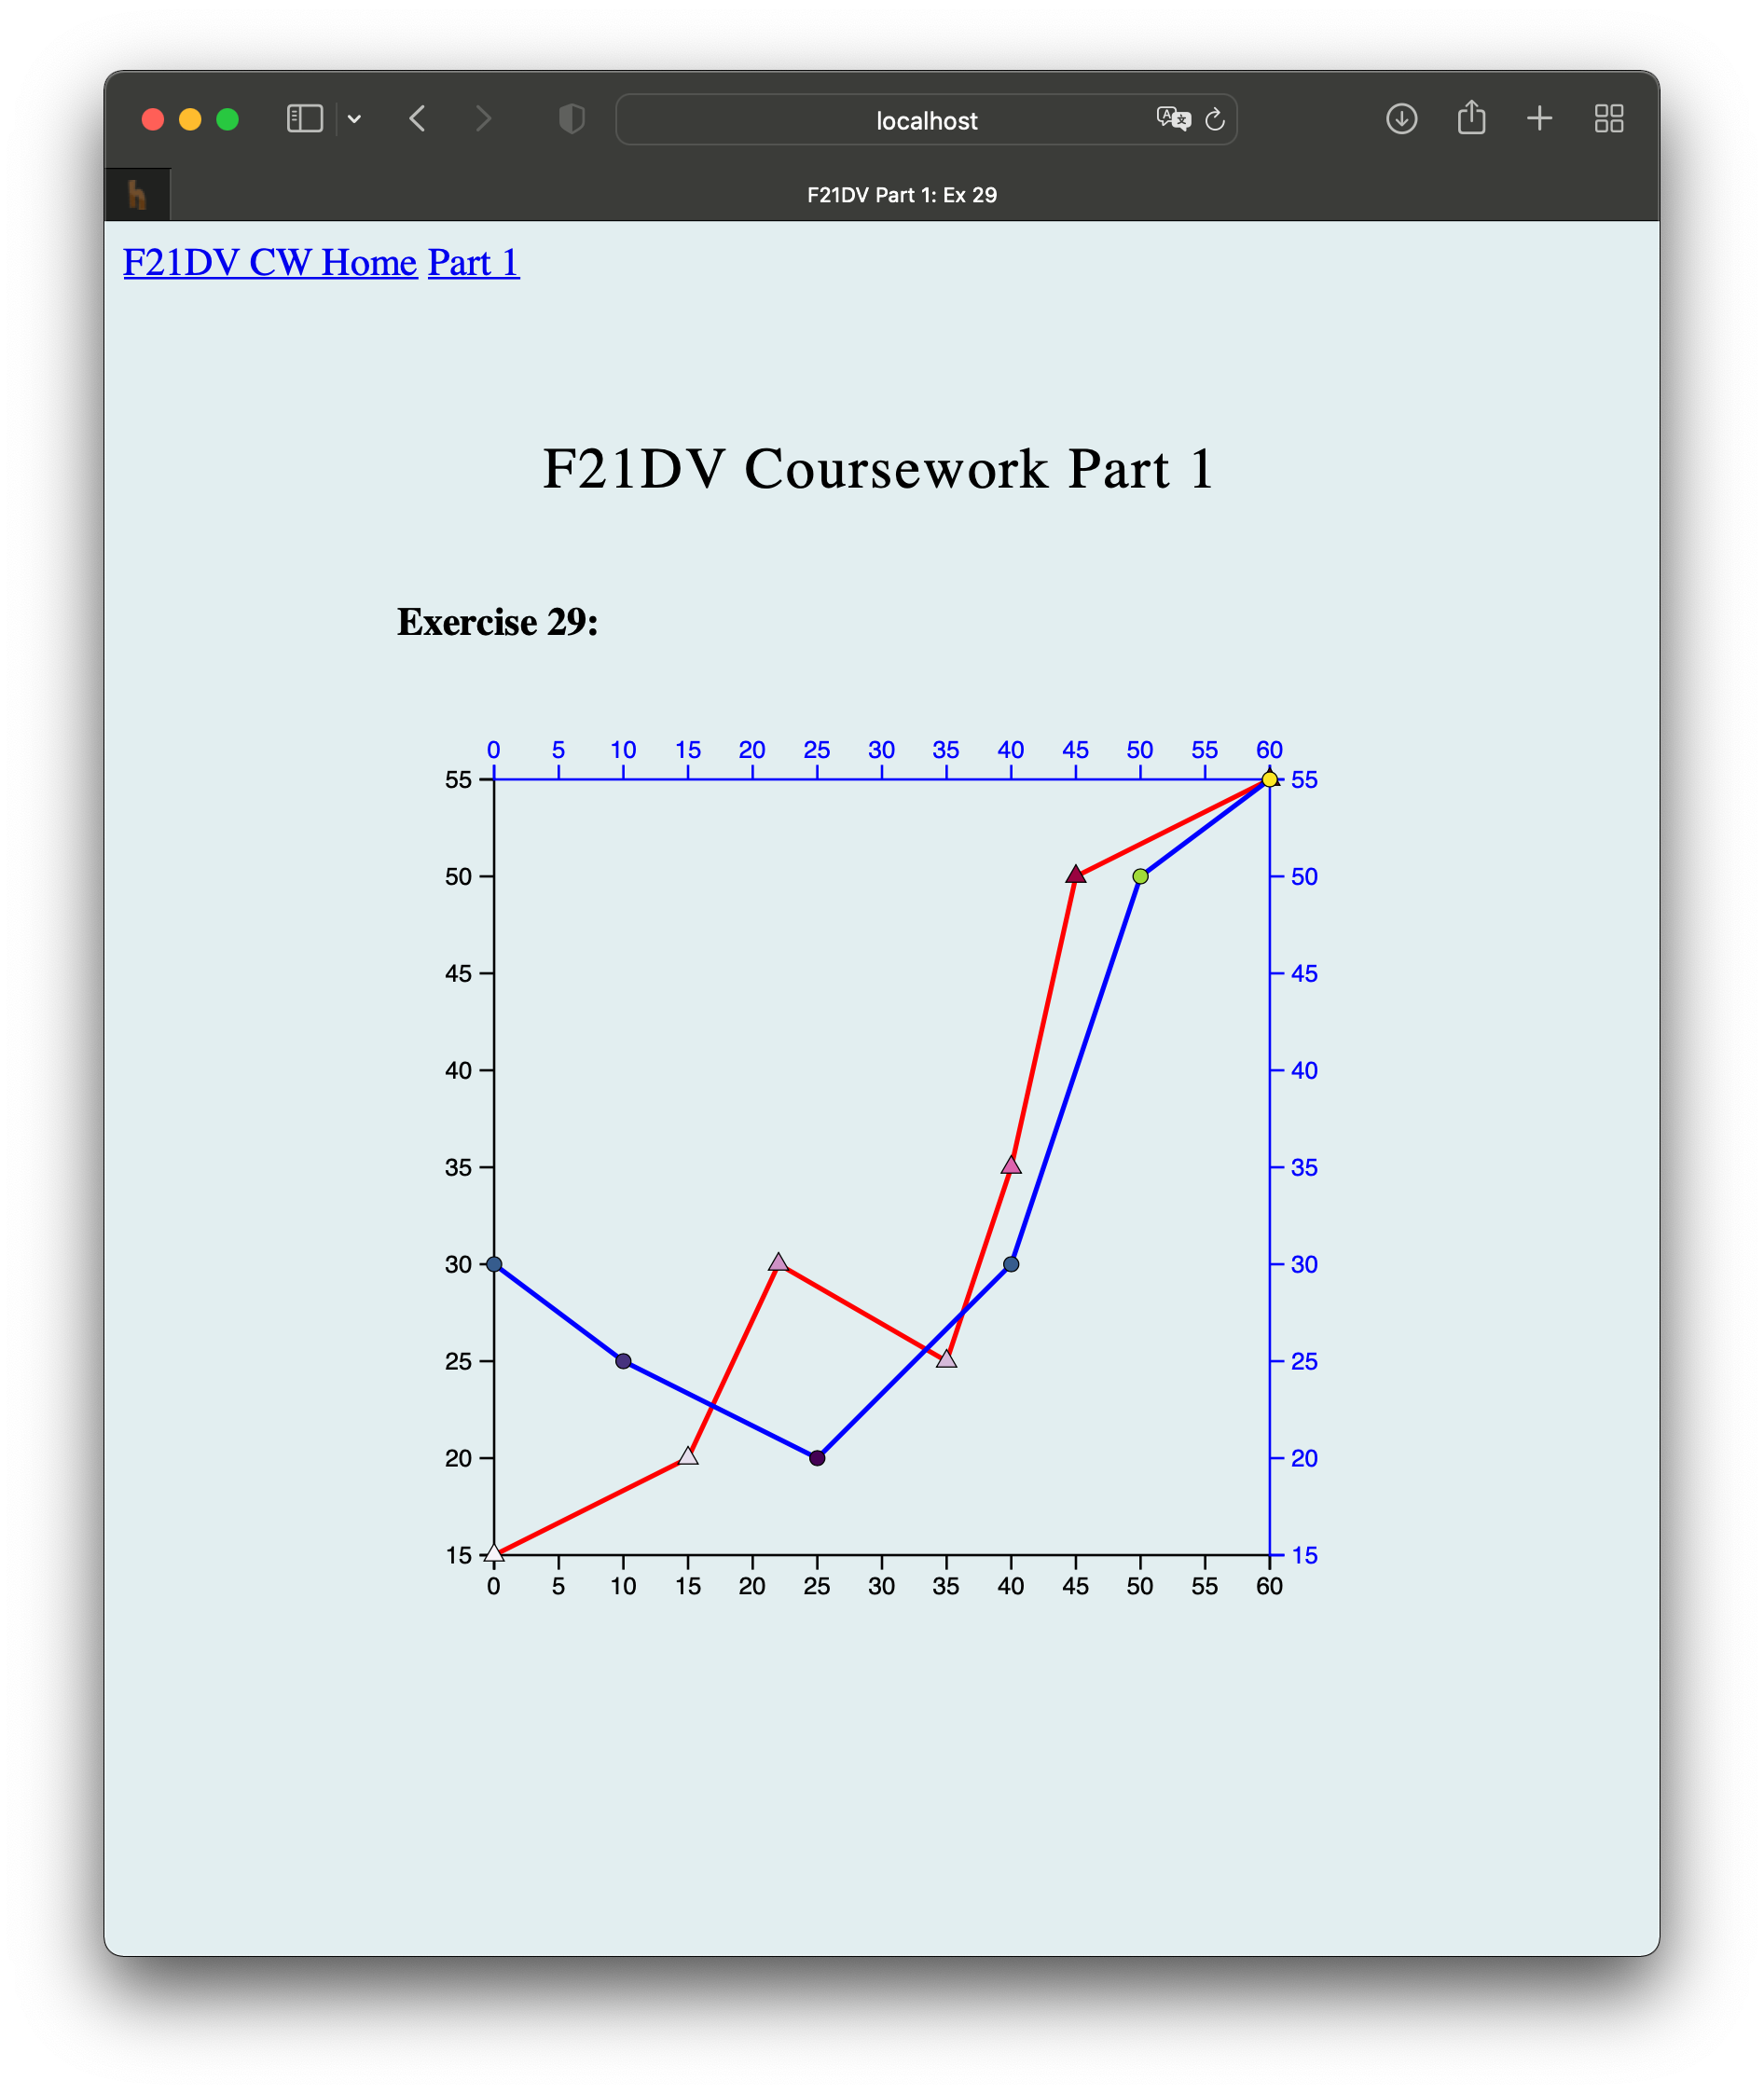
\includegraphics[width = \textwidth]{images/ex29.png}
    \label{fig:ex29}
    \caption{Exercise 29}
\end{figure}
\FloatBarrier
% \lstinputlisting[language=JavaScript]{../../public/js/part1/task25to27.js}
This is essentially the same as exercise 25 and 26. The difference is instead of using
\verb|addLinesShape()|, we use \verb|addLinesShapeDifferentColor()|. We now add a new parameter in the
constructor of the function, defining the colour scheme to use. 

\newpage
\section{Exercise 30 \& 31}
\begin{figure}[!ht]
    \centering
    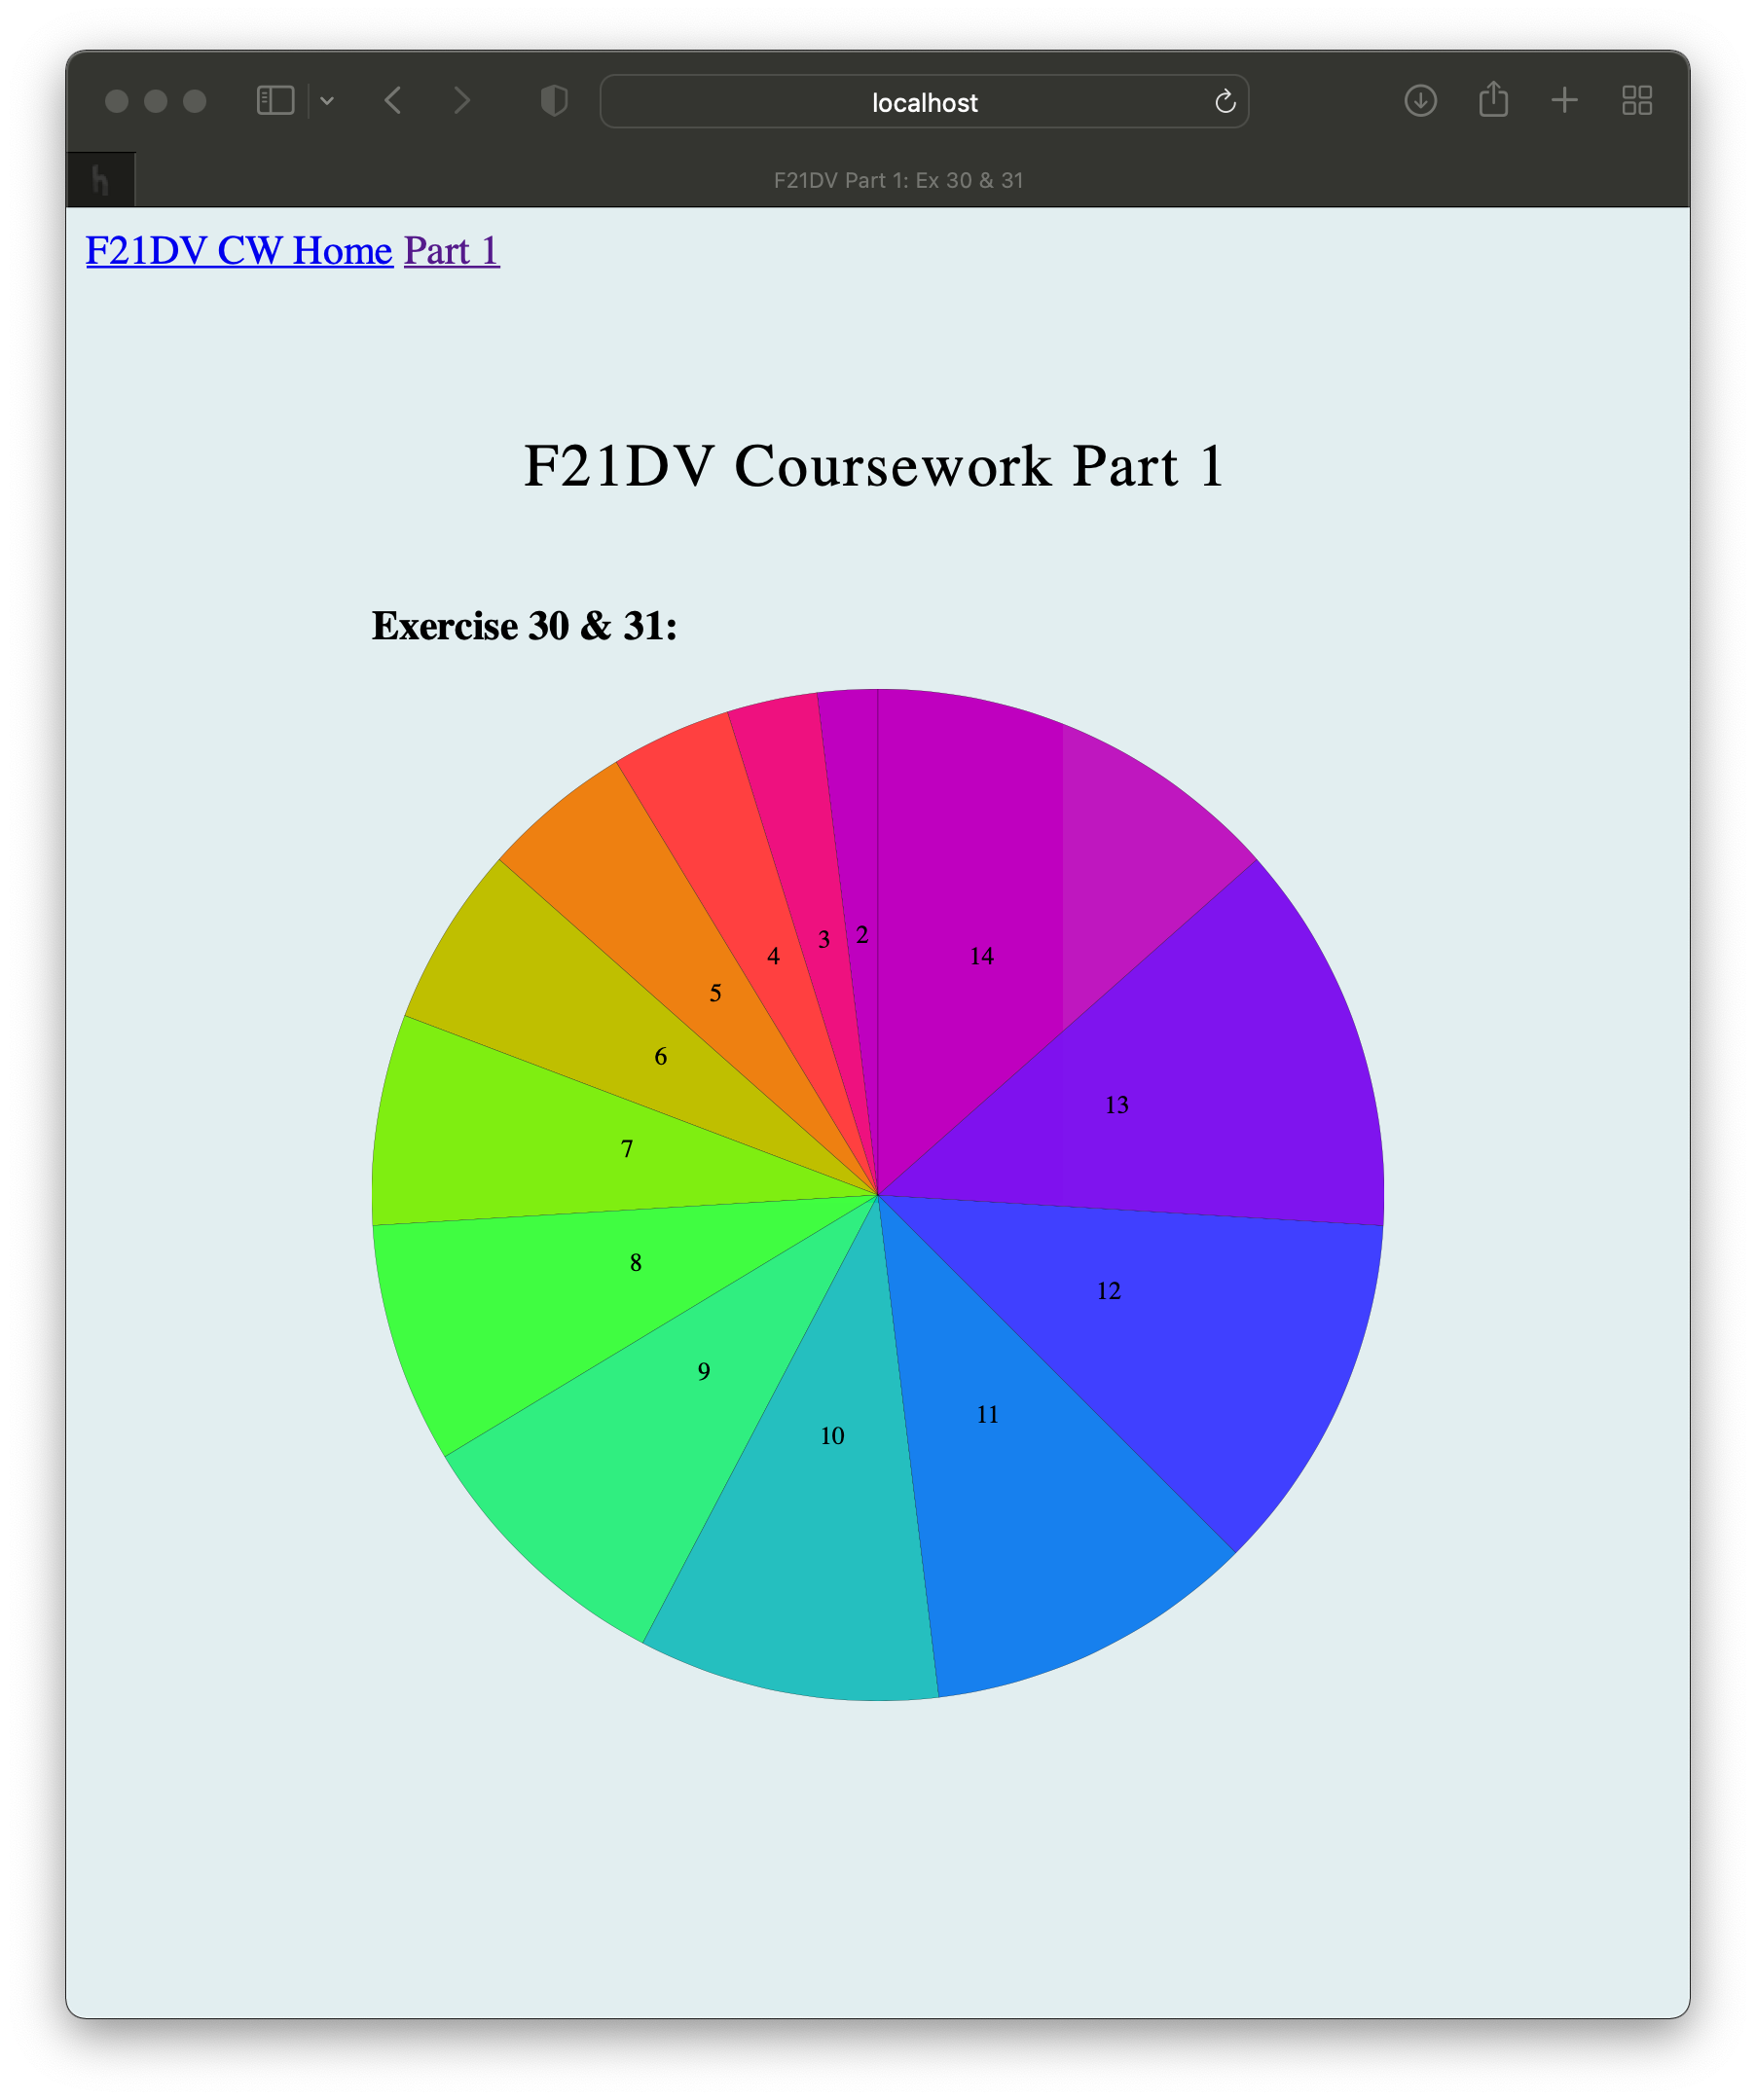
\includegraphics[width = 8cm]{images/ex30.png}
    \label{fig:ex30}
    \caption{Exercise 30 \& 31}
\end{figure}
\FloatBarrier
\lstinputlisting[language=JavaScript]{../../public/js/part1/task30n31.js}
The difference between this and earlier svgs is that this one scales using an additional arc scale.
The shape that we append is now arc, we use the same scale to transform the text for each arc as well.

\newpage
\section{Exercise 32}
\begin{figure}[!ht]
    \centering
    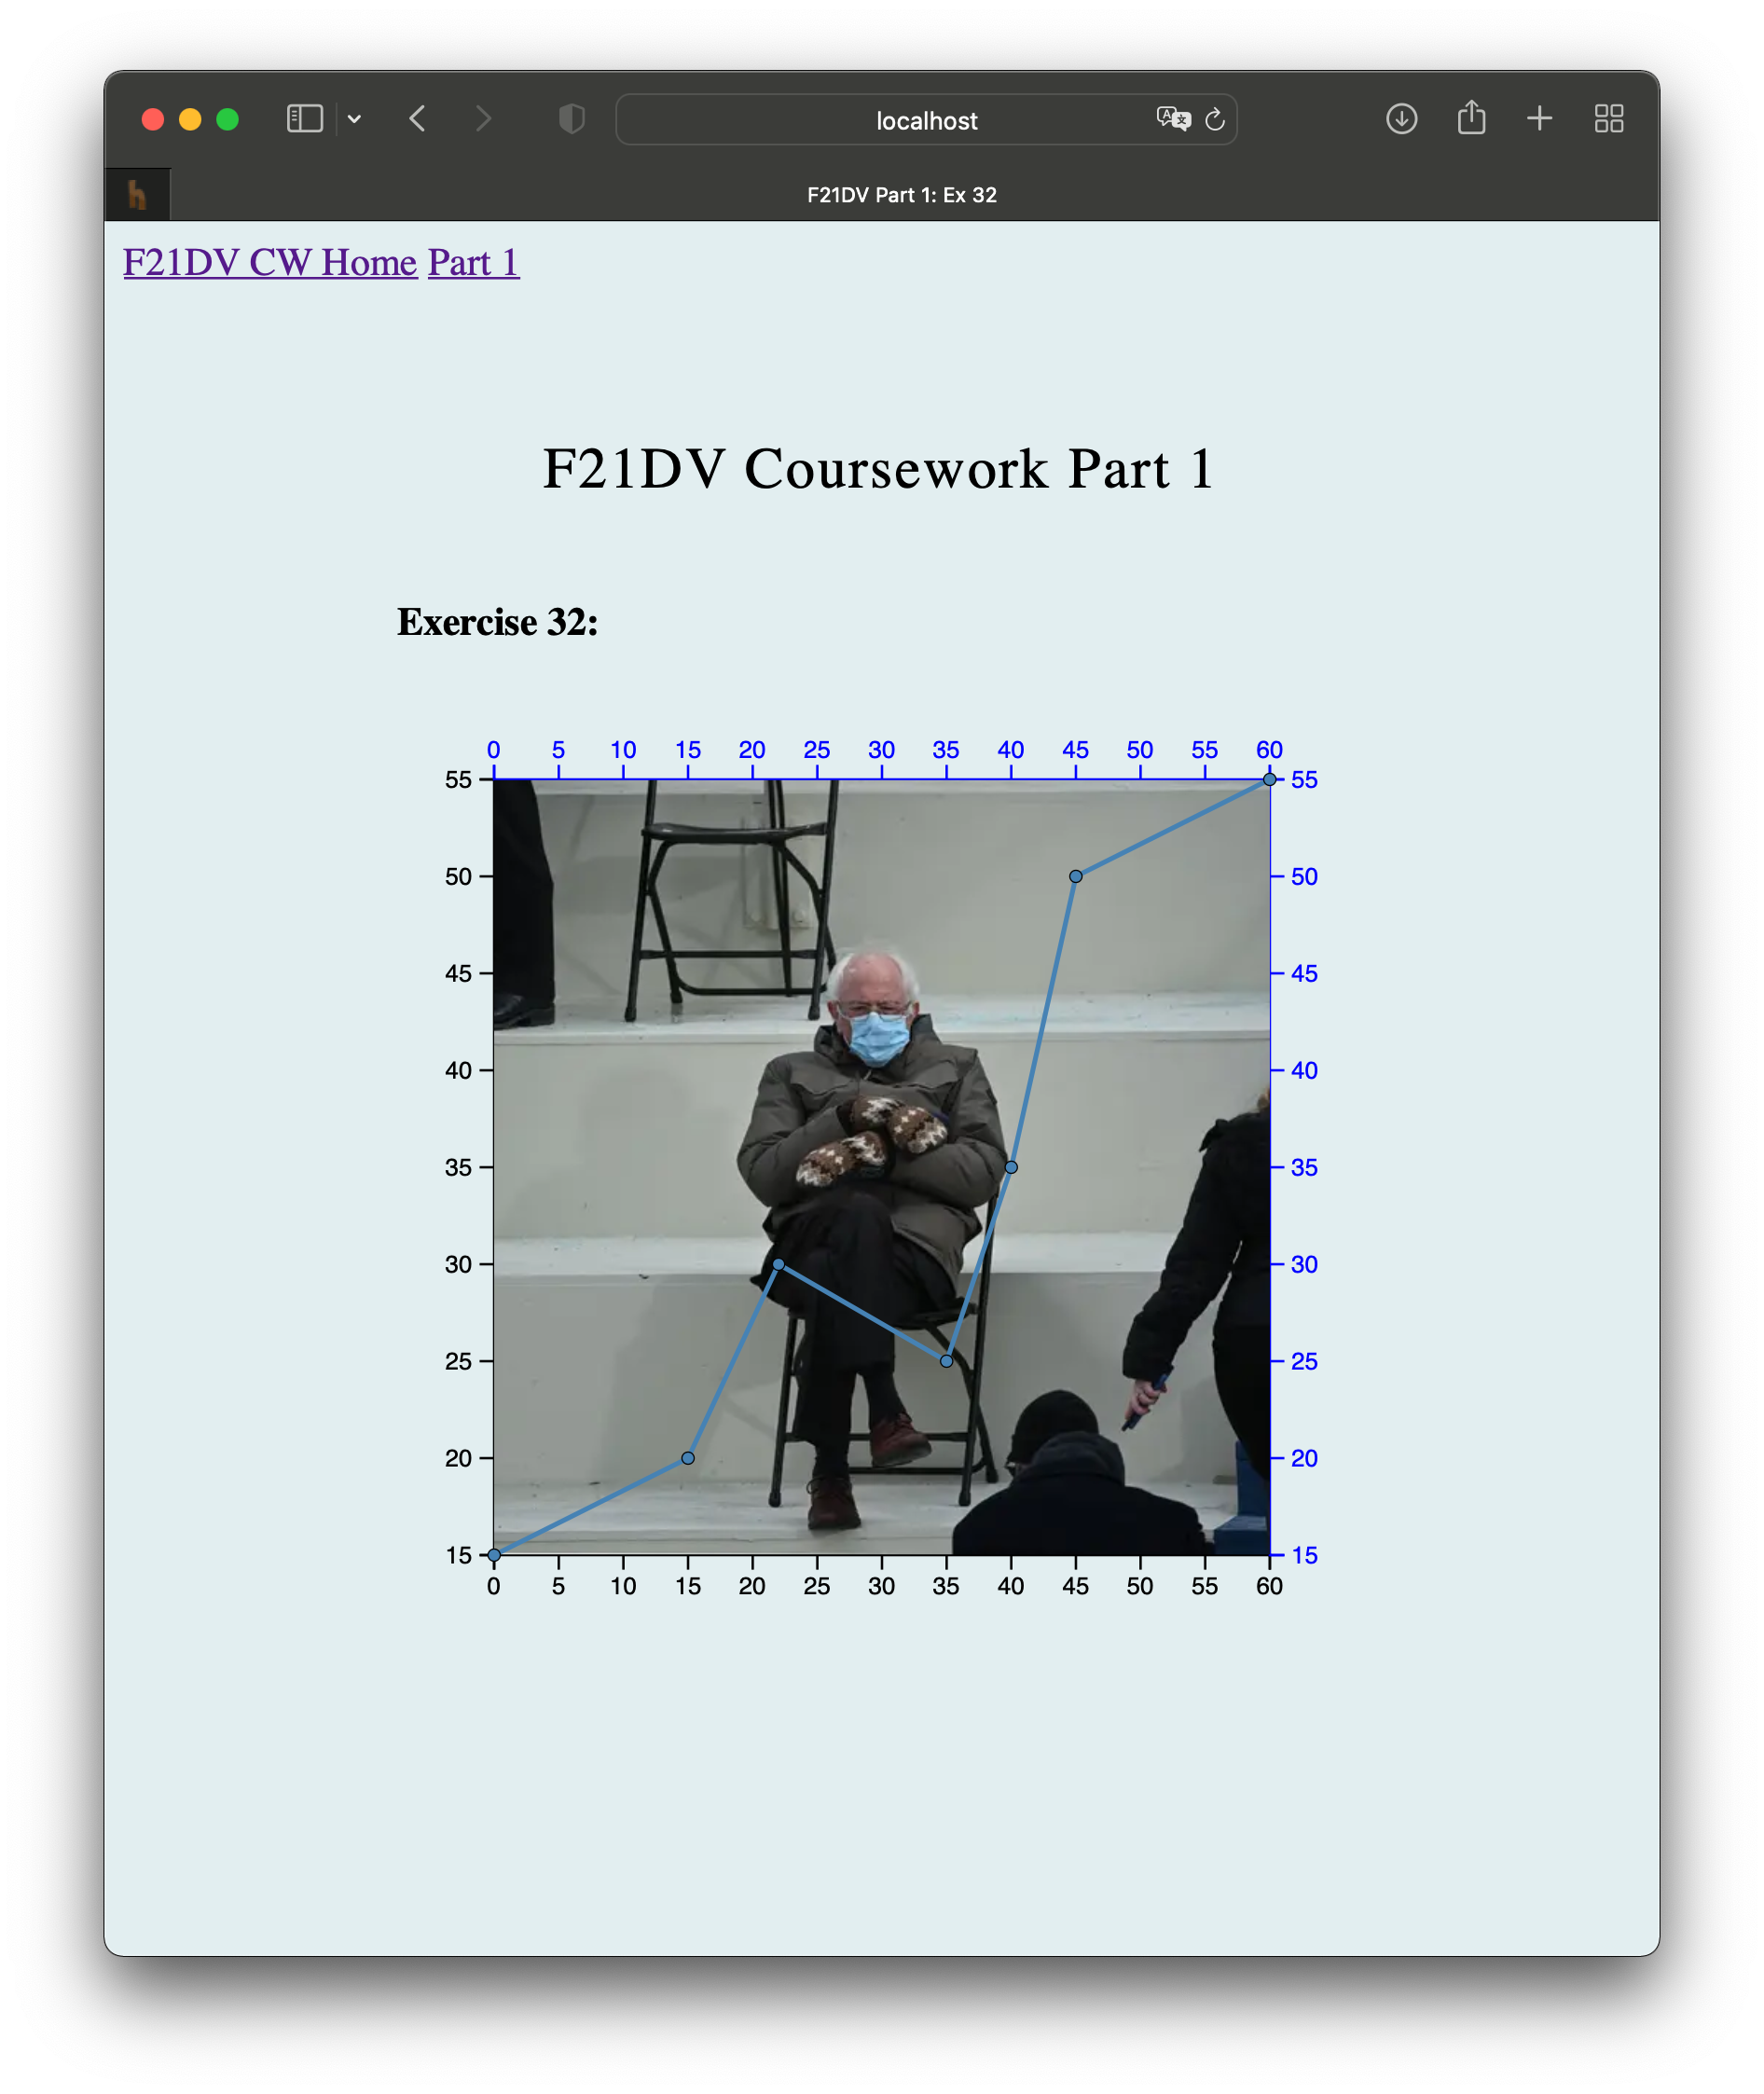
\includegraphics[width = 8cm]{images/ex32.png}
    \label{fig:ex32}
    \caption{Exercise 32}
\end{figure}
\FloatBarrier
\lstinputlisting[language=JavaScript]{../../public/js/part1/task32.js}
Now exercise 32 is pretty much an exercise 23. Difference is now we add an image before plotting the lines.


\end{document}
